\documentclass{article}
\usepackage{tikz}
\usepackage[top=1cm,left=1cm,right=1cm,bottom=1cm,landscape]{geometry}
\begin{document}

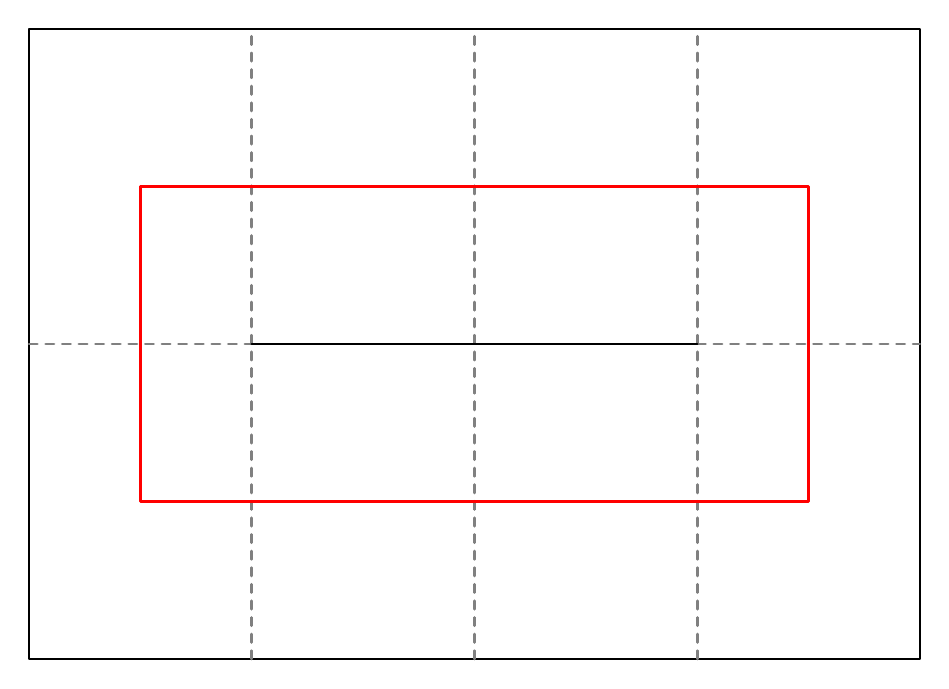
\begin{tikzpicture}[x=1.41421356cm,y=1cm,line width=1pt,line cap=round,line join=round]
\draw (0,0) rectangle (8,8);
\draw[dashed,gray]
(2,0) -- (2,8)
(4,0) -- (4,8)
(6,0) -- (6,8)
(0,4) -- (2,4) (6,4) -- (8,4);
\draw (2,4) -- (6,4);
\draw[red] (1,2) -- (1,6) -- (7,6) -- (7,2) -- cycle; 
\end{tikzpicture}
\hspace{5mm}
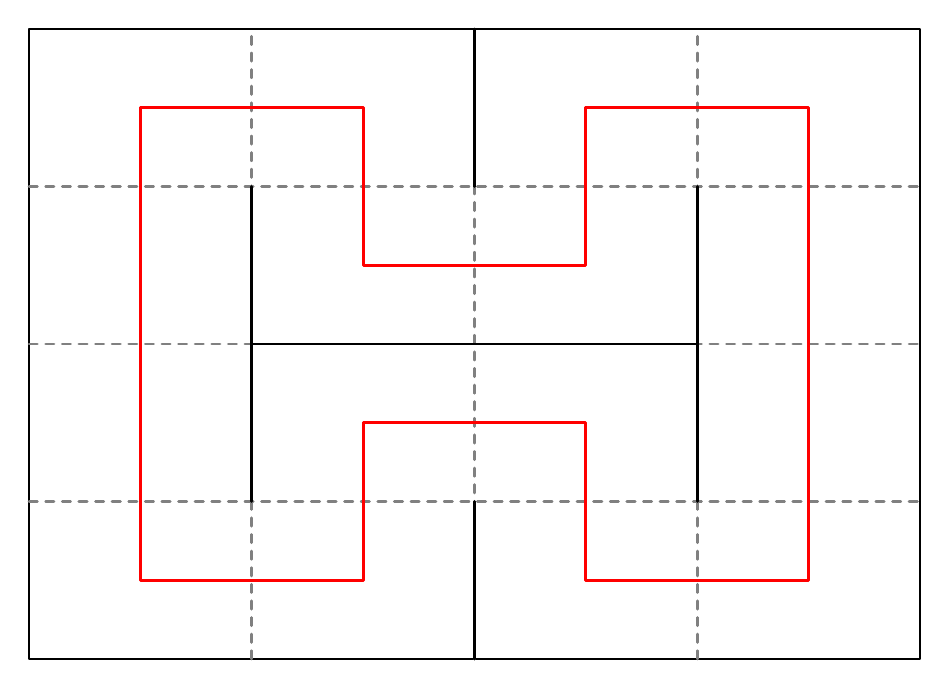
\begin{tikzpicture}[x=1.41421356cm,y=1cm,line width=1pt,line cap=round,line join=round]
\draw (0,0) rectangle (8,8);
\draw[dashed,gray]
(2,0) -- (2,8)
(4,0) -- (4,8)
(6,0) -- (6,8)
(0,2) -- (8,2)
(0,4) -- (8,4)
(0,6) -- (8,6);
\draw (2,4) -- (6,4) (2,2) -- (2,6) (4,0) -- (4,2) (4,6) -- (4,8) (6,2) -- (6,6);
\draw[red] (1,1) -- (1,7) -- (3,7) -- (3,5) -- (5,5) -- (5,7) -- (7,7) -- (7,1) -- (5,1) -- (5,3) -- (3,3) -- (3,1) -- cycle; 
\end{tikzpicture}

\vspace{5mm}

Choices:

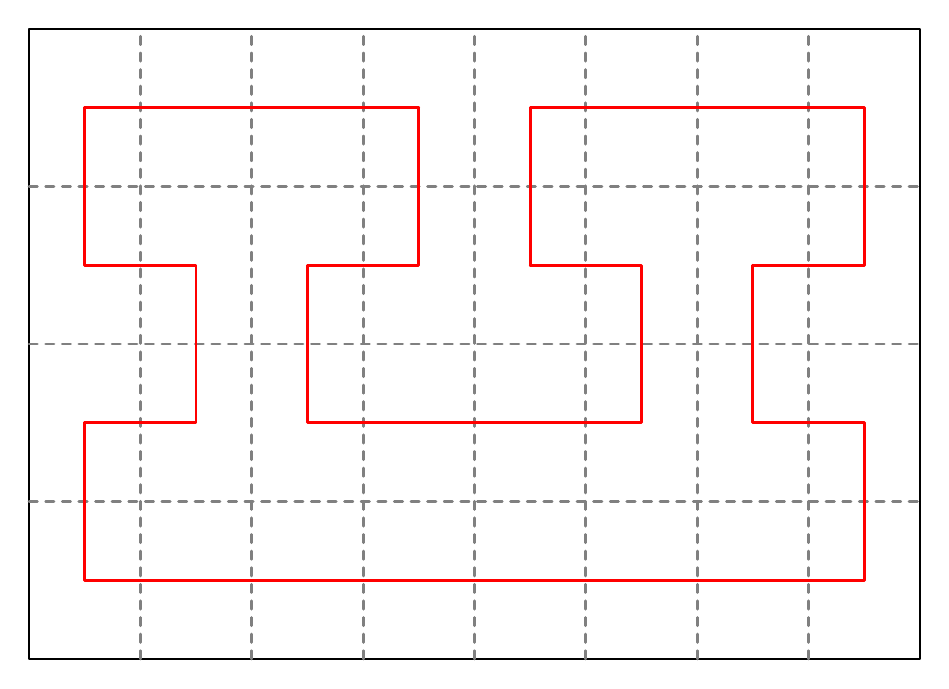
\begin{tikzpicture}[x=1.41421356cm,y=1cm,line width=1pt,line cap=round,line join=round]
\draw (0,0) rectangle (8,8);
\draw[dashed,gray]
(1,0) -- (1,8)
(2,0) -- (2,8)
(3,0) -- (3,8)
(4,0) -- (4,8)
(5,0) -- (5,8)
(6,0) -- (6,8)
(7,0) -- (7,8)
(0,2) -- (8,2)
(0,4) -- (8,4)
(0,6) -- (8,6);
%\draw (2,4) -- (6,4);
\draw[red]
    (5.5,1) -- (0.5,1) -- (0.5,3) -- (1.5,3) --
    (1.5,5) -- (0.5,5) -- (0.5,7) -- (3.5,7)
    (4.5,3) -- (2.5,3) -- (2.5,5) -- (3.5,5) -- (3.5,7)
    (5.5,1) -- (7.5,1) -- (7.5,3) -- (6.5,3) -- (6.5,5)
    (6.5,5) -- (7.5,5) -- (7.5,7) -- (4.5,7) -- (4.5,5)
    (4.5,5) -- (5.5,5) -- (5.5,3) -- (4.5,3);
\end{tikzpicture}
\hspace{5mm}
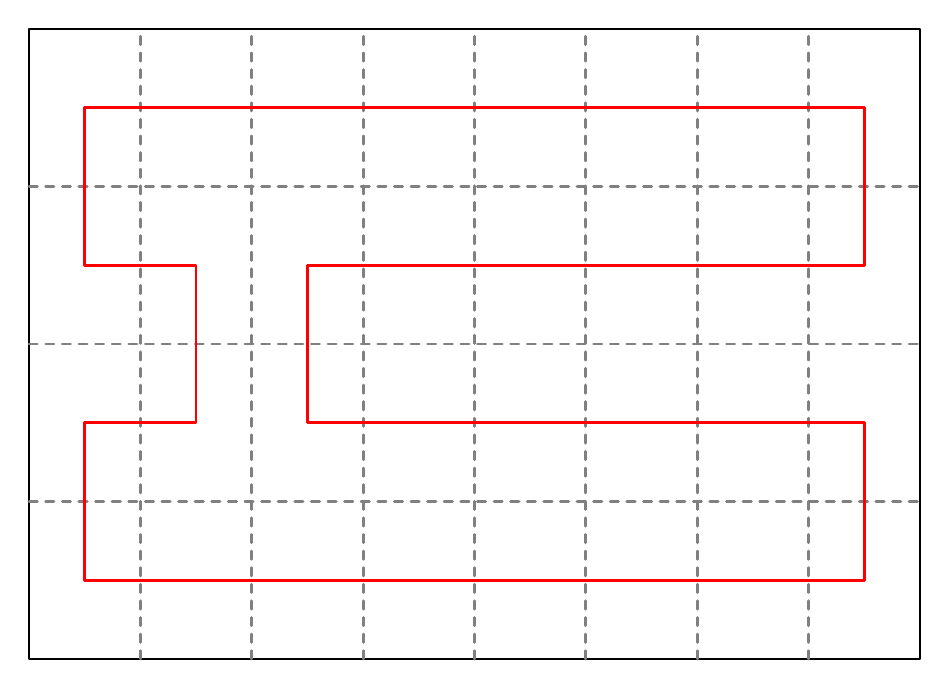
\begin{tikzpicture}[x=1.41421356cm,y=1cm,line width=1pt,line cap=round,line join=round]
\draw (0,0) rectangle (8,8);
\draw[dashed,gray]
(1,0) -- (1,8)
(2,0) -- (2,8)
(3,0) -- (3,8)
(4,0) -- (4,8)
(5,0) -- (5,8)
(6,0) -- (6,8)
(7,0) -- (7,8)
(0,2) -- (8,2)
(0,4) -- (8,4)
(0,6) -- (8,6);
%\draw (2,4) -- (6,4);
\draw[red]
    (3.5,1) -- (0.5,1) -- (0.5,3) -- (1.5,3) --
    (1.5,5) -- (0.5,5) -- (0.5,7) -- (5.5,7)
    (3.5,3) -- (2.5,3) -- (2.5,5) -- (3.5,5) -- (5.5,5)
    (3.5,1) -- (7.5,1) -- (7.5,3) -- (3.5,3)
    (5.5,5) -- (7.5,5) -- (7.5,7) -- (5.5,7);
\end{tikzpicture}

\vspace{5mm}

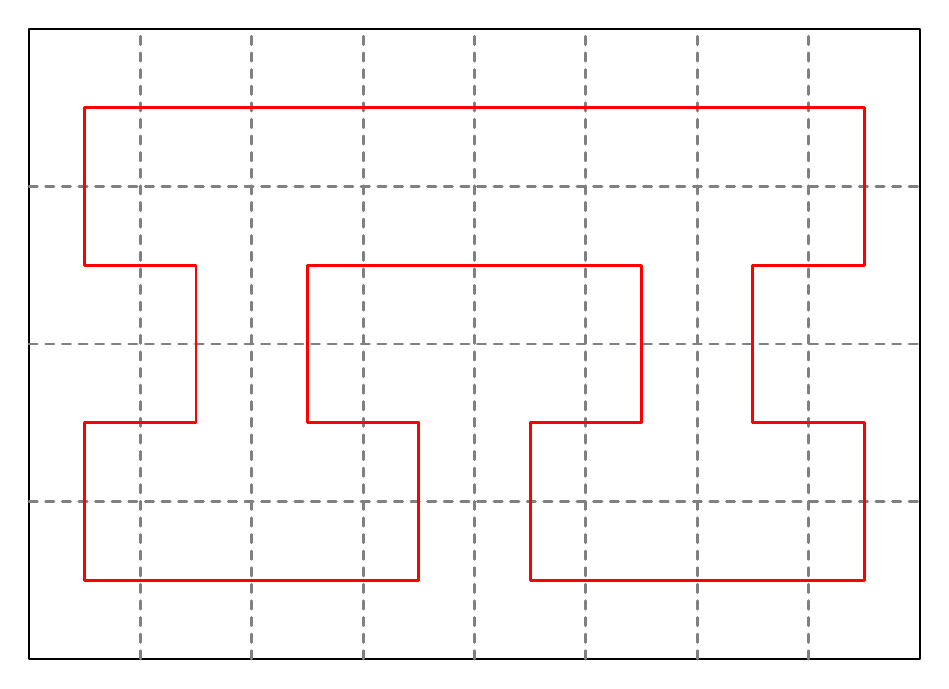
\begin{tikzpicture}[x=1.41421356cm,y=1cm,line width=1pt,line cap=round,line join=round]
\draw (0,0) rectangle (8,8);
\draw[dashed,gray]
(1,0) -- (1,8)
(2,0) -- (2,8)
(3,0) -- (3,8)
(4,0) -- (4,8)
(5,0) -- (5,8)
(6,0) -- (6,8)
(7,0) -- (7,8)
(0,2) -- (8,2)
(0,4) -- (8,4)
(0,6) -- (8,6);
%\draw (2,4) -- (6,4);
\draw[red]
    (3.5,3) -- (3.5,1) -- (0.5,1) -- (0.5,3) -- (1.5,3) --
    (1.5,5) -- (0.5,5) -- (0.5,7) -- (5.5,7)
    (3.5,3) -- (2.5,3) -- (2.5,5) -- (3.5,5) -- (5.5,5) -- (5.5,3)
    (5.5,1) -- (7.5,1) -- (7.5,3) -- (6.5,3)
    (6.5,3) -- (6.5,5) -- (7.5,5) -- (7.5,7) -- (5.5,7)
    (5.5,3) -- (4.5,3) -- (4.5,1) -- (5.5,1);
\end{tikzpicture}
\hspace{5mm}
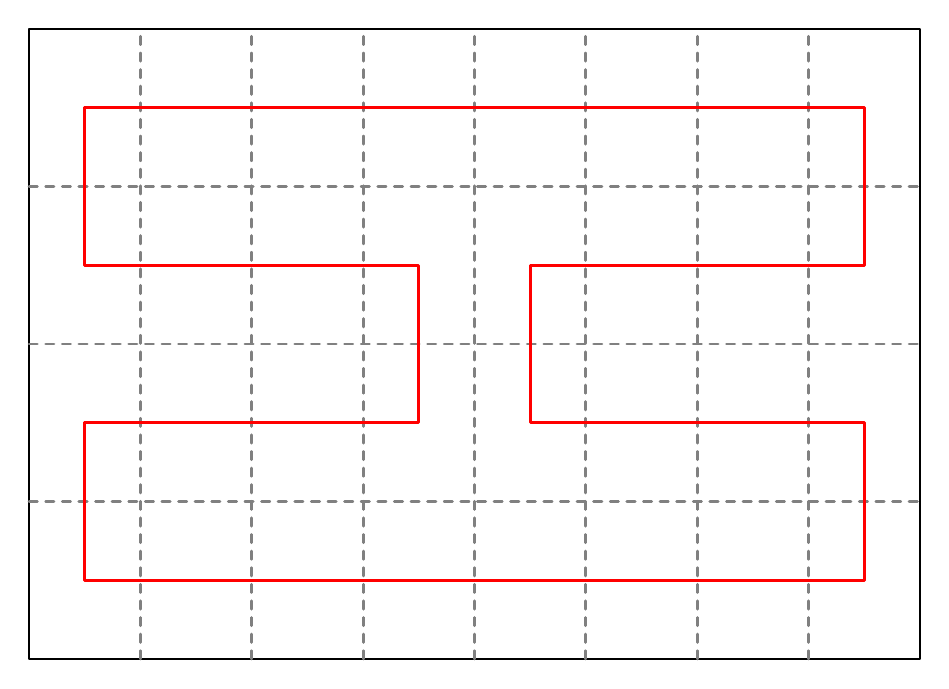
\begin{tikzpicture}[x=1.41421356cm,y=1cm,line width=1pt,line cap=round,line join=round]
\draw (0,0) rectangle (8,8);
\draw[dashed,gray]
(1,0) -- (1,8)
(2,0) -- (2,8)
(3,0) -- (3,8)
(4,0) -- (4,8)
(5,0) -- (5,8)
(6,0) -- (6,8)
(7,0) -- (7,8)
(0,2) -- (8,2)
(0,4) -- (8,4)
(0,6) -- (8,6);
%\draw (2,4) -- (6,4);
\draw[red]
    (5.5,1) -- (0.5,1) -- (0.5,3) -- (3.5,3) -- 
    (3.5,5) -- (0.5,5) -- (0.5,7) -- (5.5,7)
    (5.5,1) -- (7.5,1) -- (7.5,3) -- (6.5,3)
    (6.5,3) -- (4.5,3) -- (4.5,5) -- (7.5,5) -- (7.5,7) -- (5.5,7);
\end{tikzpicture}

\vspace{5mm}

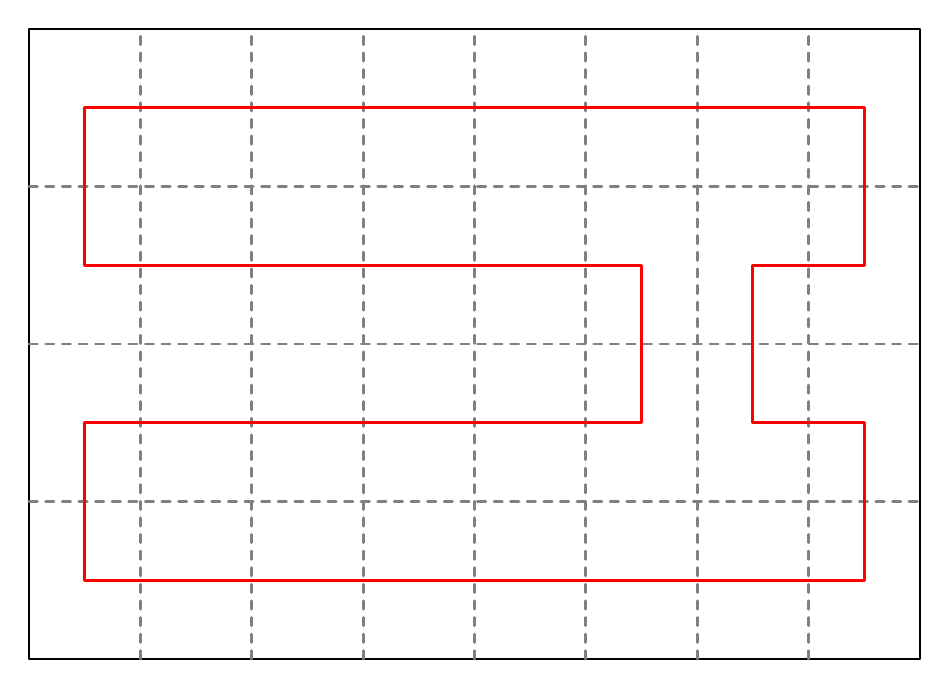
\begin{tikzpicture}[x=1.41421356cm,y=1cm,line width=1pt,line cap=round,line join=round]
\draw (0,0) rectangle (8,8);
\draw[dashed,gray]
(1,0) -- (1,8)
(2,0) -- (2,8)
(3,0) -- (3,8)
(4,0) -- (4,8)
(5,0) -- (5,8)
(6,0) -- (6,8)
(7,0) -- (7,8)
(0,2) -- (8,2)
(0,4) -- (8,4)
(0,6) -- (8,6);
%\draw (2,4) -- (6,4);
\draw[red]
    (5.5,1) -- (0.5,1) -- (0.5,3) -- (5.5,3) --
    (5.5,5) -- (0.5,5) -- (0.5,7) -- (5.5,7)
    (5.5,1) -- (7.5,1) -- (7.5,3) -- (6.5,3)
    (6.5,3) -- (6.5,5) -- (7.5,5) -- (7.5,7) -- (5.5,7);
\end{tikzpicture}

Should be invalid:
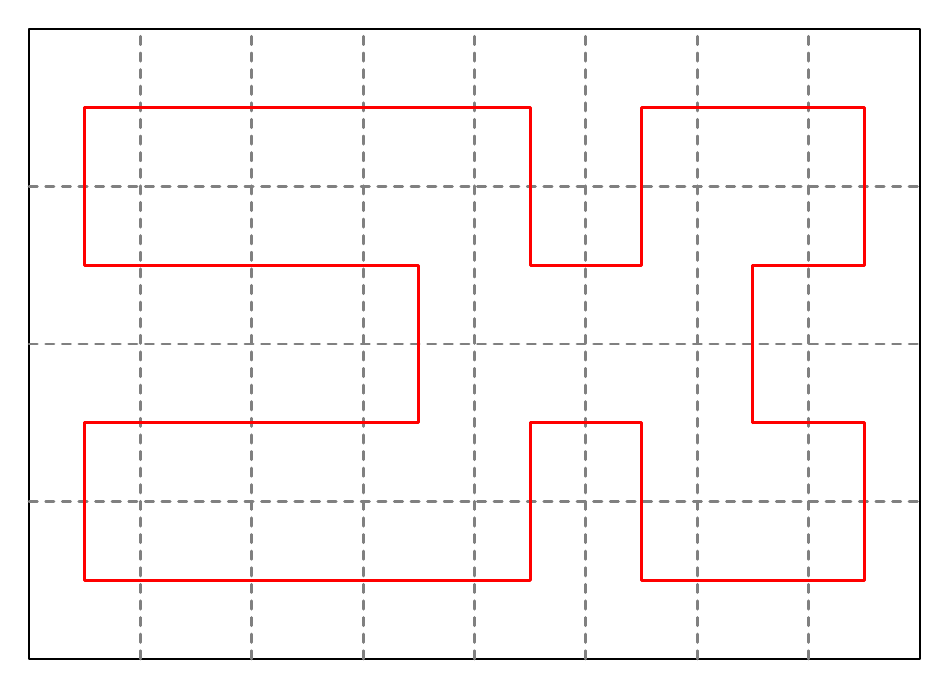
\begin{tikzpicture}[x=1.41421356cm,y=1cm,line width=1pt,line cap=round,line join=round]
\draw (0,0) rectangle (8,8);
\draw[dashed,gray]
(1,0) -- (1,8)
(2,0) -- (2,8)
(3,0) -- (3,8)
(4,0) -- (4,8)
(5,0) -- (5,8)
(6,0) -- (6,8)
(7,0) -- (7,8)
(0,2) -- (8,2)
(0,4) -- (8,4)
(0,6) -- (8,6);
%\draw (2,4) -- (6,4);
\draw[red]
    (4.5,1) -- (0.5,1) -- (0.5,3) -- (3.5,3) -- 
    (3.5,5) -- (0.5,5) -- (0.5,7) -- (4.5,7) -- (4.5,5) -- (5.5,5) -- (5.5,7)
    (4.5,1) -- (4.5,3) -- (5.5,3) -- (5.5,1) -- (7.5,1) -- (7.5,3) -- (6.5,3)
    (6.5,3) -- (6.5,5) -- (7.5,5) -- (7.5,7) -- (5.5,7);
\end{tikzpicture}

\newpage

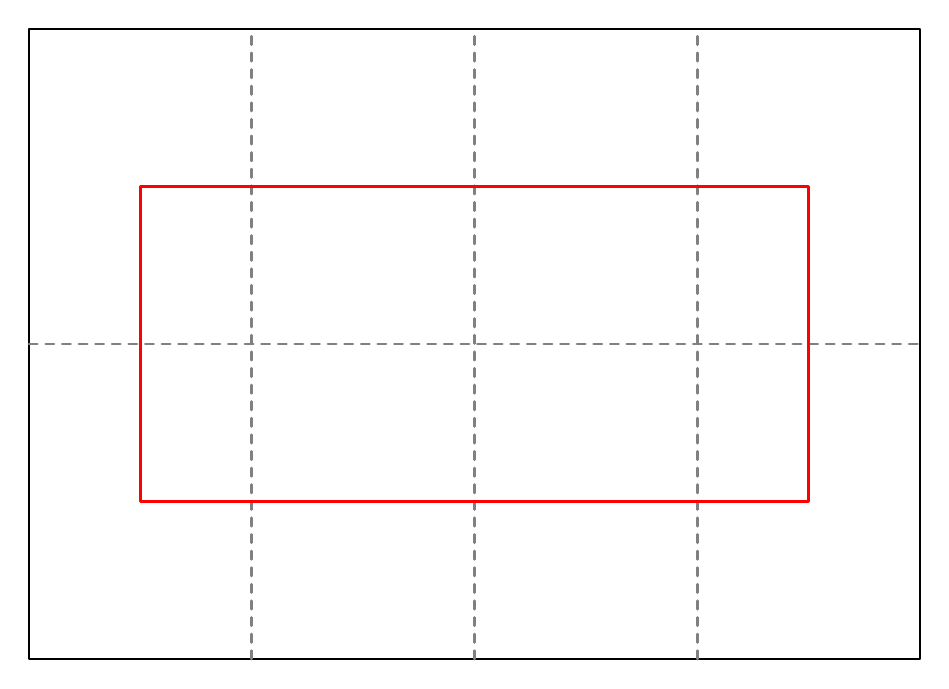
\begin{tikzpicture}[x=2.8284271247461903cm,y=4.0cm,line width=1pt,line cap=round,line join=round]
\draw (0,0) rectangle (4,2);
\draw[dashed,gray] (1,0) -- (1,2) (2,0) -- (2,2) (3,0) -- (3,2) (0,1) -- (4,1);
\draw[red] (0.5,0.5) -- (1.5,0.5) -- (2.5,0.5) -- (3.5,0.5) -- (3.5,1.5) -- (2.5,1.5) -- (1.5,1.5) -- (0.5,1.5) -- (0.5,0.5) -- cycle;\end{tikzpicture}
\hspace{5mm}
\newpage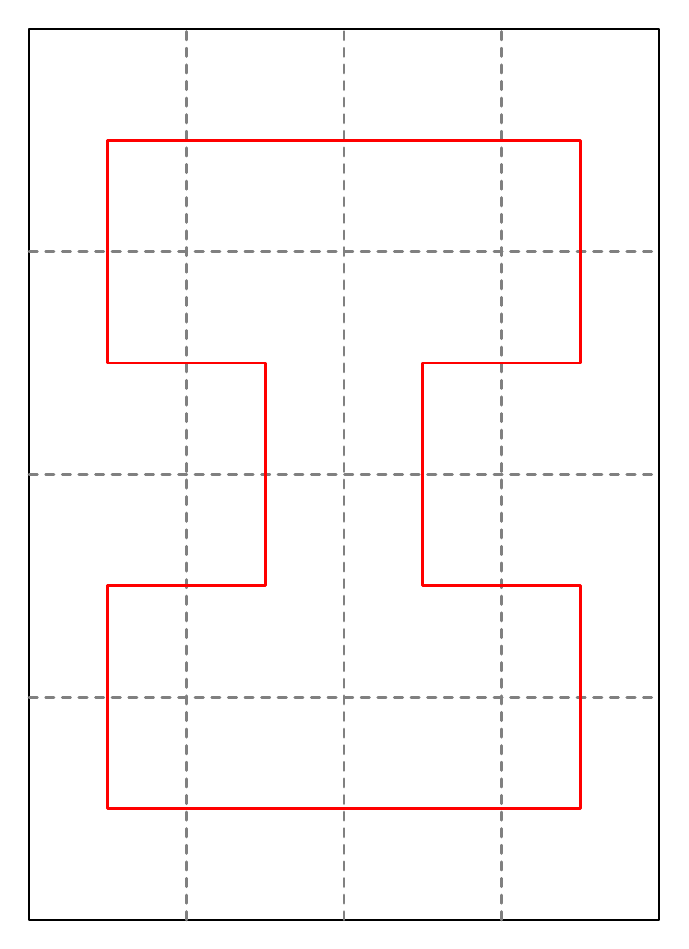
\begin{tikzpicture}[x=2.0cm,y=2.8284271247461903cm,line width=1pt,line cap=round,line join=round]
\draw (0,0) rectangle (4,4);
\draw[dashed,gray] (1,0) -- (1,4) (2,0) -- (2,4) (3,0) -- (3,4) (0,1) -- (4,1) (0,2) -- (4,2) (0,3) -- (4,3);
\draw[red] (0.5,0.5) -- (1.5,0.5) -- (2.5,0.5) -- (3.5,0.5) -- (3.5,1.5) -- (2.5,1.5) -- (2.5,2.5) -- (3.5,2.5) -- (3.5,3.5) -- (2.5,3.5) -- (1.5,3.5) -- (0.5,3.5) -- (0.5,2.5) -- (1.5,2.5) -- (1.5,1.5) -- (0.5,1.5) -- (0.5,0.5) -- cycle;\end{tikzpicture}
\hspace{5mm}
\newpage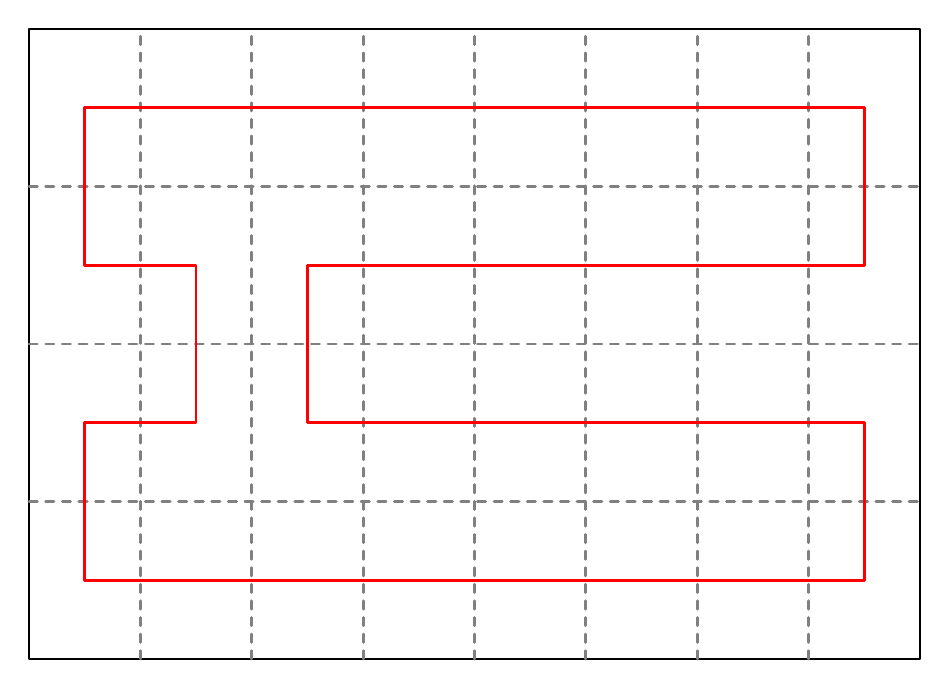
\begin{tikzpicture}[x=1.4142135623730951cm,y=2.0cm,line width=1pt,line cap=round,line join=round]
\draw (0,0) rectangle (8,4);
\draw[dashed,gray] (1,0) -- (1,4) (2,0) -- (2,4) (3,0) -- (3,4) (4,0) -- (4,4) (5,0) -- (5,4) (6,0) -- (6,4) (7,0) -- (7,4) (0,1) -- (8,1) (0,2) -- (8,2) (0,3) -- (8,3);
\draw[red] (0.5,0.5) -- (1.5,0.5) -- (2.5,0.5) -- (3.5,0.5) -- (4.5,0.5) -- (5.5,0.5) -- (6.5,0.5) -- (7.5,0.5) -- (7.5,1.5) -- (6.5,1.5) -- (5.5,1.5) -- (4.5,1.5) -- (3.5,1.5) -- (2.5,1.5) -- (2.5,2.5) -- (3.5,2.5) -- (4.5,2.5) -- (5.5,2.5) -- (6.5,2.5) -- (7.5,2.5) -- (7.5,3.5) -- (6.5,3.5) -- (5.5,3.5) -- (4.5,3.5) -- (3.5,3.5) -- (2.5,3.5) -- (1.5,3.5) -- (0.5,3.5) -- (0.5,2.5) -- (1.5,2.5) -- (1.5,1.5) -- (0.5,1.5) -- (0.5,0.5) -- cycle;\end{tikzpicture}
\hspace{5mm}
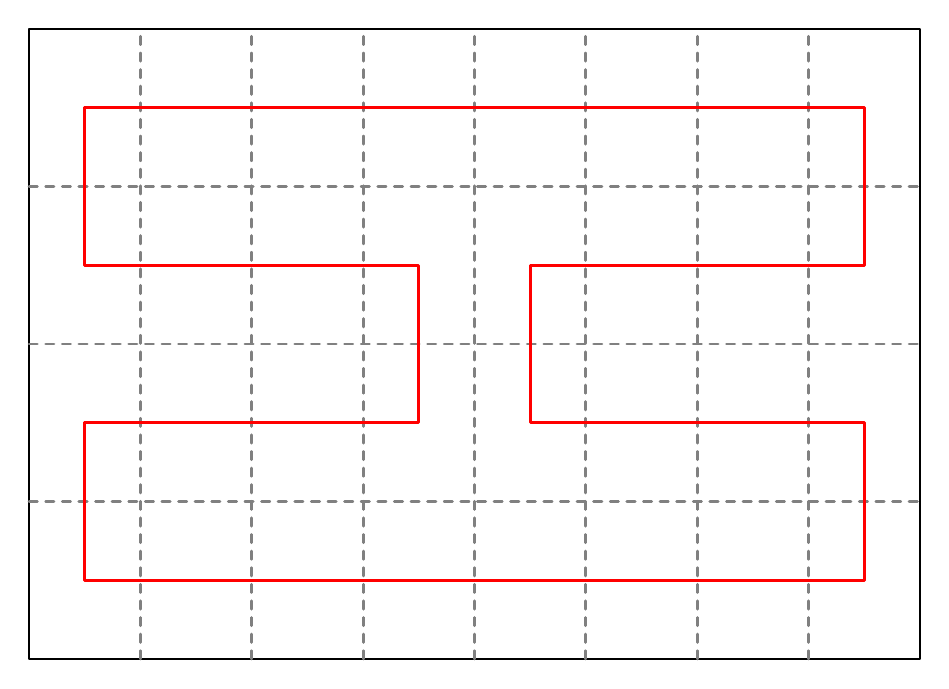
\begin{tikzpicture}[x=1.4142135623730951cm,y=2.0cm,line width=1pt,line cap=round,line join=round]
\draw (0,0) rectangle (8,4);
\draw[dashed,gray] (1,0) -- (1,4) (2,0) -- (2,4) (3,0) -- (3,4) (4,0) -- (4,4) (5,0) -- (5,4) (6,0) -- (6,4) (7,0) -- (7,4) (0,1) -- (8,1) (0,2) -- (8,2) (0,3) -- (8,3);
\draw[red] (0.5,0.5) -- (1.5,0.5) -- (2.5,0.5) -- (3.5,0.5) -- (4.5,0.5) -- (5.5,0.5) -- (6.5,0.5) -- (7.5,0.5) -- (7.5,1.5) -- (6.5,1.5) -- (5.5,1.5) -- (4.5,1.5) -- (4.5,2.5) -- (5.5,2.5) -- (6.5,2.5) -- (7.5,2.5) -- (7.5,3.5) -- (6.5,3.5) -- (5.5,3.5) -- (4.5,3.5) -- (3.5,3.5) -- (2.5,3.5) -- (1.5,3.5) -- (0.5,3.5) -- (0.5,2.5) -- (1.5,2.5) -- (2.5,2.5) -- (3.5,2.5) -- (3.5,1.5) -- (2.5,1.5) -- (1.5,1.5) -- (0.5,1.5) -- (0.5,0.5) -- cycle;\end{tikzpicture}

\vspace{5mm}

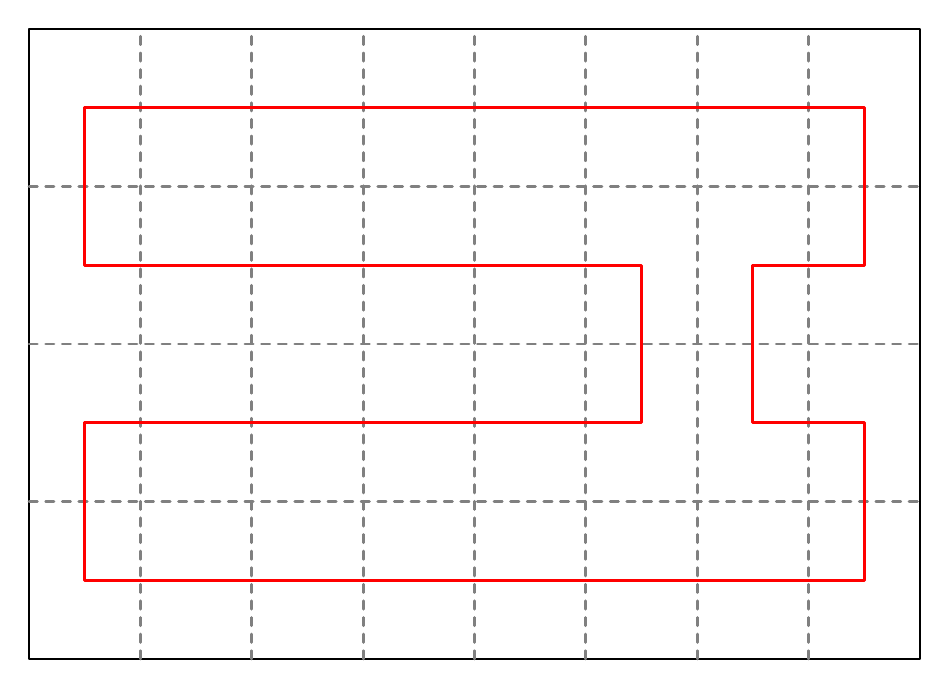
\begin{tikzpicture}[x=1.4142135623730951cm,y=2.0cm,line width=1pt,line cap=round,line join=round]
\draw (0,0) rectangle (8,4);
\draw[dashed,gray] (1,0) -- (1,4) (2,0) -- (2,4) (3,0) -- (3,4) (4,0) -- (4,4) (5,0) -- (5,4) (6,0) -- (6,4) (7,0) -- (7,4) (0,1) -- (8,1) (0,2) -- (8,2) (0,3) -- (8,3);
\draw[red] (0.5,0.5) -- (1.5,0.5) -- (2.5,0.5) -- (3.5,0.5) -- (4.5,0.5) -- (5.5,0.5) -- (6.5,0.5) -- (7.5,0.5) -- (7.5,1.5) -- (6.5,1.5) -- (6.5,2.5) -- (7.5,2.5) -- (7.5,3.5) -- (6.5,3.5) -- (5.5,3.5) -- (4.5,3.5) -- (3.5,3.5) -- (2.5,3.5) -- (1.5,3.5) -- (0.5,3.5) -- (0.5,2.5) -- (1.5,2.5) -- (2.5,2.5) -- (3.5,2.5) -- (4.5,2.5) -- (5.5,2.5) -- (5.5,1.5) -- (4.5,1.5) -- (3.5,1.5) -- (2.5,1.5) -- (1.5,1.5) -- (0.5,1.5) -- (0.5,0.5) -- cycle;\end{tikzpicture}
\hspace{5mm}
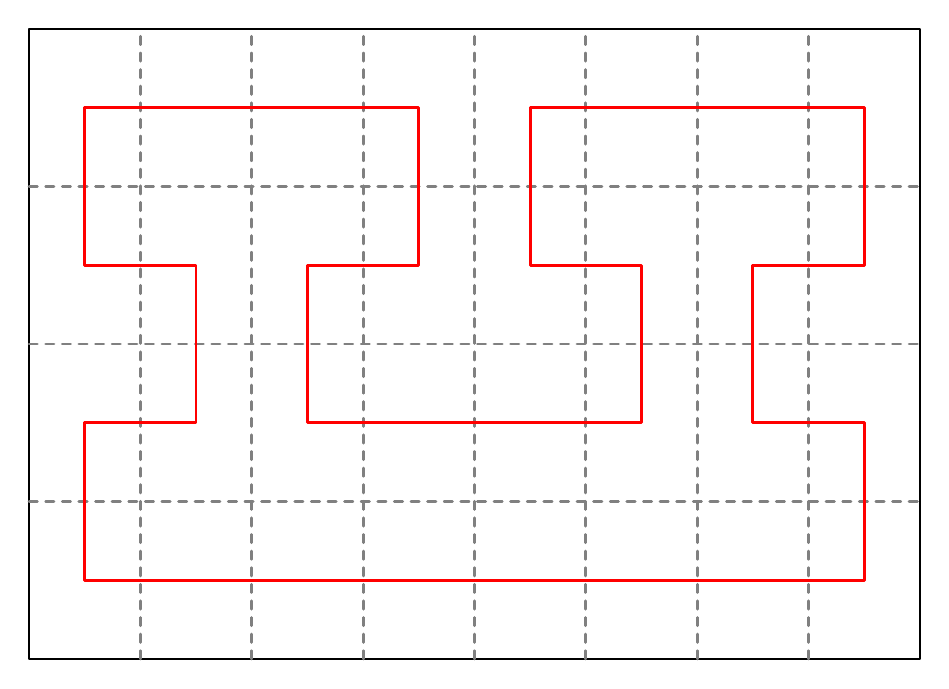
\begin{tikzpicture}[x=1.4142135623730951cm,y=2.0cm,line width=1pt,line cap=round,line join=round]
\draw (0,0) rectangle (8,4);
\draw[dashed,gray] (1,0) -- (1,4) (2,0) -- (2,4) (3,0) -- (3,4) (4,0) -- (4,4) (5,0) -- (5,4) (6,0) -- (6,4) (7,0) -- (7,4) (0,1) -- (8,1) (0,2) -- (8,2) (0,3) -- (8,3);
\draw[red] (0.5,0.5) -- (1.5,0.5) -- (2.5,0.5) -- (3.5,0.5) -- (4.5,0.5) -- (5.5,0.5) -- (6.5,0.5) -- (7.5,0.5) -- (7.5,1.5) -- (6.5,1.5) -- (6.5,2.5) -- (7.5,2.5) -- (7.5,3.5) -- (6.5,3.5) -- (5.5,3.5) -- (4.5,3.5) -- (4.5,2.5) -- (5.5,2.5) -- (5.5,1.5) -- (4.5,1.5) -- (3.5,1.5) -- (2.5,1.5) -- (2.5,2.5) -- (3.5,2.5) -- (3.5,3.5) -- (2.5,3.5) -- (1.5,3.5) -- (0.5,3.5) -- (0.5,2.5) -- (1.5,2.5) -- (1.5,1.5) -- (0.5,1.5) -- (0.5,0.5) -- cycle;\end{tikzpicture}

\vspace{5mm}

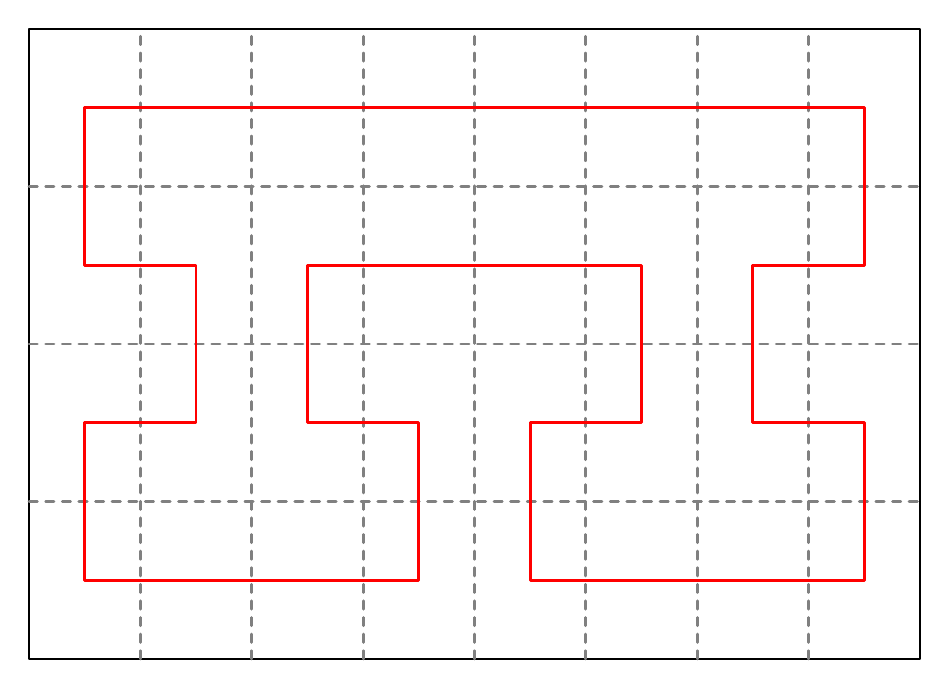
\begin{tikzpicture}[x=1.4142135623730951cm,y=2.0cm,line width=1pt,line cap=round,line join=round]
\draw (0,0) rectangle (8,4);
\draw[dashed,gray] (1,0) -- (1,4) (2,0) -- (2,4) (3,0) -- (3,4) (4,0) -- (4,4) (5,0) -- (5,4) (6,0) -- (6,4) (7,0) -- (7,4) (0,1) -- (8,1) (0,2) -- (8,2) (0,3) -- (8,3);
\draw[red] (0.5,0.5) -- (1.5,0.5) -- (2.5,0.5) -- (3.5,0.5) -- (3.5,1.5) -- (2.5,1.5) -- (2.5,2.5) -- (3.5,2.5) -- (4.5,2.5) -- (5.5,2.5) -- (5.5,1.5) -- (4.5,1.5) -- (4.5,0.5) -- (5.5,0.5) -- (6.5,0.5) -- (7.5,0.5) -- (7.5,1.5) -- (6.5,1.5) -- (6.5,2.5) -- (7.5,2.5) -- (7.5,3.5) -- (6.5,3.5) -- (5.5,3.5) -- (4.5,3.5) -- (3.5,3.5) -- (2.5,3.5) -- (1.5,3.5) -- (0.5,3.5) -- (0.5,2.5) -- (1.5,2.5) -- (1.5,1.5) -- (0.5,1.5) -- (0.5,0.5) -- cycle;\end{tikzpicture}
\hspace{5mm}
\newpage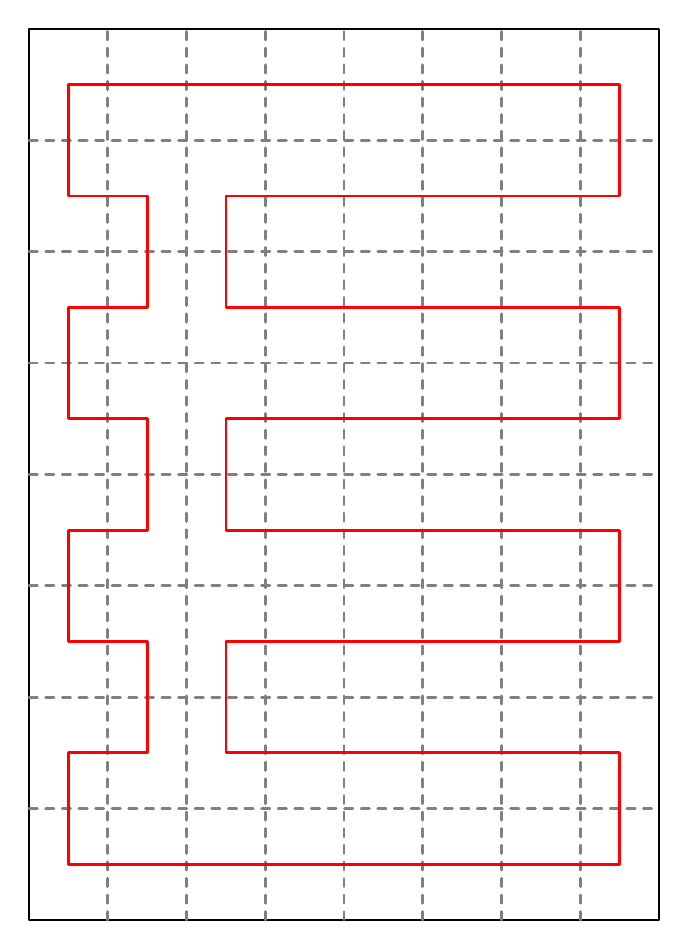
\begin{tikzpicture}[x=1.0cm,y=1.4142135623730951cm,line width=1pt,line cap=round,line join=round]
\draw (0,0) rectangle (8,8);
\draw[dashed,gray] (1,0) -- (1,8) (2,0) -- (2,8) (3,0) -- (3,8) (4,0) -- (4,8) (5,0) -- (5,8) (6,0) -- (6,8) (7,0) -- (7,8) (0,1) -- (8,1) (0,2) -- (8,2) (0,3) -- (8,3) (0,4) -- (8,4) (0,5) -- (8,5) (0,6) -- (8,6) (0,7) -- (8,7);
\draw[red] (0.5,0.5) -- (1.5,0.5) -- (2.5,0.5) -- (3.5,0.5) -- (4.5,0.5) -- (5.5,0.5) -- (6.5,0.5) -- (7.5,0.5) -- (7.5,1.5) -- (6.5,1.5) -- (5.5,1.5) -- (4.5,1.5) -- (3.5,1.5) -- (2.5,1.5) -- (2.5,2.5) -- (3.5,2.5) -- (4.5,2.5) -- (5.5,2.5) -- (6.5,2.5) -- (7.5,2.5) -- (7.5,3.5) -- (6.5,3.5) -- (5.5,3.5) -- (4.5,3.5) -- (3.5,3.5) -- (2.5,3.5) -- (2.5,4.5) -- (3.5,4.5) -- (4.5,4.5) -- (5.5,4.5) -- (6.5,4.5) -- (7.5,4.5) -- (7.5,5.5) -- (6.5,5.5) -- (5.5,5.5) -- (4.5,5.5) -- (3.5,5.5) -- (2.5,5.5) -- (2.5,6.5) -- (3.5,6.5) -- (4.5,6.5) -- (5.5,6.5) -- (6.5,6.5) -- (7.5,6.5) -- (7.5,7.5) -- (6.5,7.5) -- (5.5,7.5) -- (4.5,7.5) -- (3.5,7.5) -- (2.5,7.5) -- (1.5,7.5) -- (0.5,7.5) -- (0.5,6.5) -- (1.5,6.5) -- (1.5,5.5) -- (0.5,5.5) -- (0.5,4.5) -- (1.5,4.5) -- (1.5,3.5) -- (0.5,3.5) -- (0.5,2.5) -- (1.5,2.5) -- (1.5,1.5) -- (0.5,1.5) -- (0.5,0.5) -- cycle;\end{tikzpicture}
\hspace{5mm}
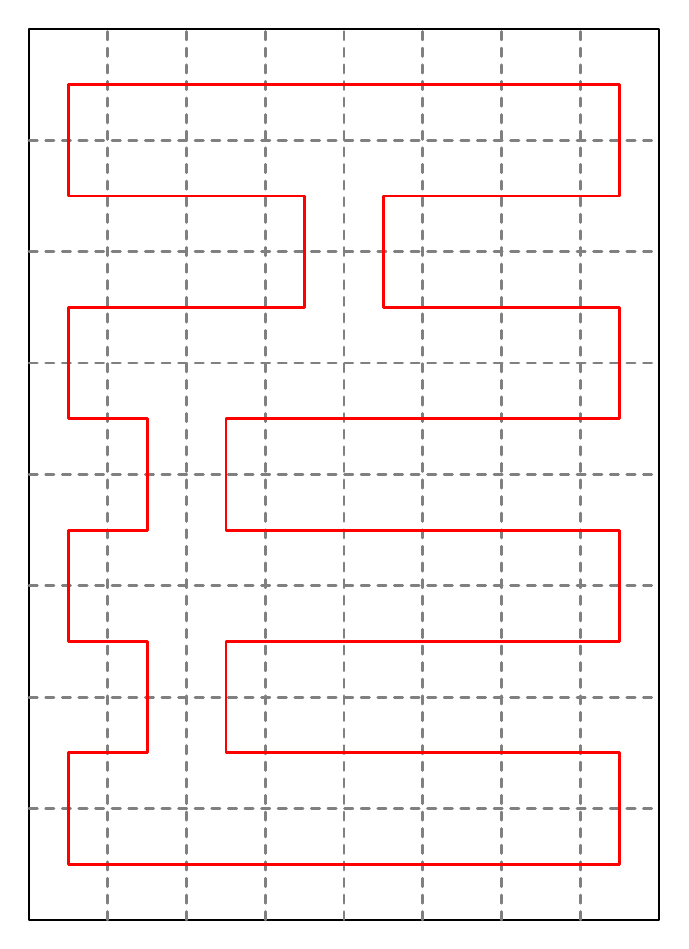
\begin{tikzpicture}[x=1.0cm,y=1.4142135623730951cm,line width=1pt,line cap=round,line join=round]
\draw (0,0) rectangle (8,8);
\draw[dashed,gray] (1,0) -- (1,8) (2,0) -- (2,8) (3,0) -- (3,8) (4,0) -- (4,8) (5,0) -- (5,8) (6,0) -- (6,8) (7,0) -- (7,8) (0,1) -- (8,1) (0,2) -- (8,2) (0,3) -- (8,3) (0,4) -- (8,4) (0,5) -- (8,5) (0,6) -- (8,6) (0,7) -- (8,7);
\draw[red] (0.5,0.5) -- (1.5,0.5) -- (2.5,0.5) -- (3.5,0.5) -- (4.5,0.5) -- (5.5,0.5) -- (6.5,0.5) -- (7.5,0.5) -- (7.5,1.5) -- (6.5,1.5) -- (5.5,1.5) -- (4.5,1.5) -- (3.5,1.5) -- (2.5,1.5) -- (2.5,2.5) -- (3.5,2.5) -- (4.5,2.5) -- (5.5,2.5) -- (6.5,2.5) -- (7.5,2.5) -- (7.5,3.5) -- (6.5,3.5) -- (5.5,3.5) -- (4.5,3.5) -- (3.5,3.5) -- (2.5,3.5) -- (2.5,4.5) -- (3.5,4.5) -- (4.5,4.5) -- (5.5,4.5) -- (6.5,4.5) -- (7.5,4.5) -- (7.5,5.5) -- (6.5,5.5) -- (5.5,5.5) -- (4.5,5.5) -- (4.5,6.5) -- (5.5,6.5) -- (6.5,6.5) -- (7.5,6.5) -- (7.5,7.5) -- (6.5,7.5) -- (5.5,7.5) -- (4.5,7.5) -- (3.5,7.5) -- (2.5,7.5) -- (1.5,7.5) -- (0.5,7.5) -- (0.5,6.5) -- (1.5,6.5) -- (2.5,6.5) -- (3.5,6.5) -- (3.5,5.5) -- (2.5,5.5) -- (1.5,5.5) -- (0.5,5.5) -- (0.5,4.5) -- (1.5,4.5) -- (1.5,3.5) -- (0.5,3.5) -- (0.5,2.5) -- (1.5,2.5) -- (1.5,1.5) -- (0.5,1.5) -- (0.5,0.5) -- cycle;\end{tikzpicture}

\vspace{5mm}

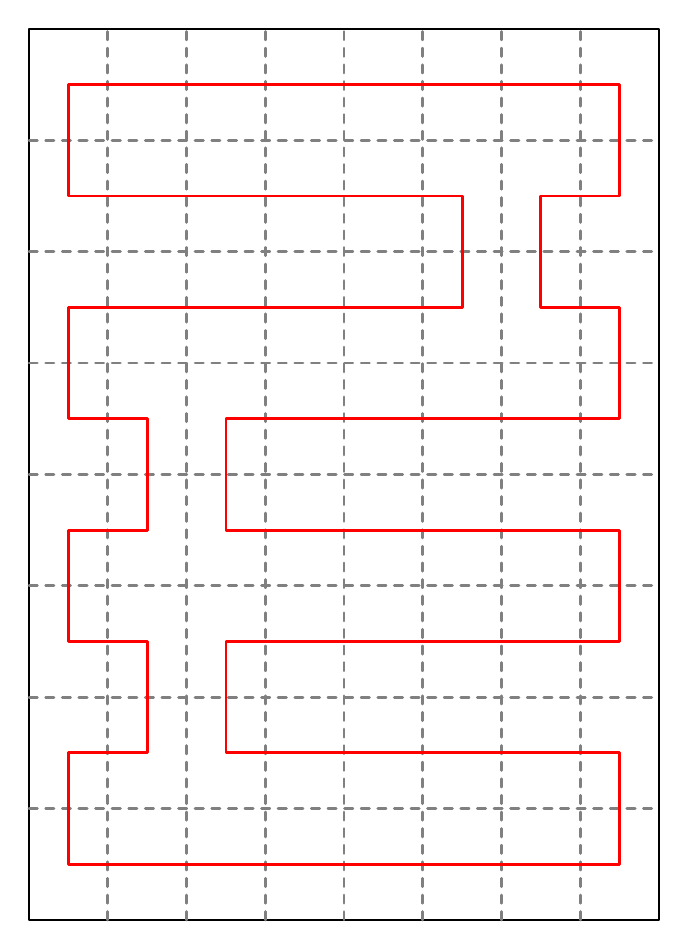
\begin{tikzpicture}[x=1.0cm,y=1.4142135623730951cm,line width=1pt,line cap=round,line join=round]
\draw (0,0) rectangle (8,8);
\draw[dashed,gray] (1,0) -- (1,8) (2,0) -- (2,8) (3,0) -- (3,8) (4,0) -- (4,8) (5,0) -- (5,8) (6,0) -- (6,8) (7,0) -- (7,8) (0,1) -- (8,1) (0,2) -- (8,2) (0,3) -- (8,3) (0,4) -- (8,4) (0,5) -- (8,5) (0,6) -- (8,6) (0,7) -- (8,7);
\draw[red] (0.5,0.5) -- (1.5,0.5) -- (2.5,0.5) -- (3.5,0.5) -- (4.5,0.5) -- (5.5,0.5) -- (6.5,0.5) -- (7.5,0.5) -- (7.5,1.5) -- (6.5,1.5) -- (5.5,1.5) -- (4.5,1.5) -- (3.5,1.5) -- (2.5,1.5) -- (2.5,2.5) -- (3.5,2.5) -- (4.5,2.5) -- (5.5,2.5) -- (6.5,2.5) -- (7.5,2.5) -- (7.5,3.5) -- (6.5,3.5) -- (5.5,3.5) -- (4.5,3.5) -- (3.5,3.5) -- (2.5,3.5) -- (2.5,4.5) -- (3.5,4.5) -- (4.5,4.5) -- (5.5,4.5) -- (6.5,4.5) -- (7.5,4.5) -- (7.5,5.5) -- (6.5,5.5) -- (6.5,6.5) -- (7.5,6.5) -- (7.5,7.5) -- (6.5,7.5) -- (5.5,7.5) -- (4.5,7.5) -- (3.5,7.5) -- (2.5,7.5) -- (1.5,7.5) -- (0.5,7.5) -- (0.5,6.5) -- (1.5,6.5) -- (2.5,6.5) -- (3.5,6.5) -- (4.5,6.5) -- (5.5,6.5) -- (5.5,5.5) -- (4.5,5.5) -- (3.5,5.5) -- (2.5,5.5) -- (1.5,5.5) -- (0.5,5.5) -- (0.5,4.5) -- (1.5,4.5) -- (1.5,3.5) -- (0.5,3.5) -- (0.5,2.5) -- (1.5,2.5) -- (1.5,1.5) -- (0.5,1.5) -- (0.5,0.5) -- cycle;\end{tikzpicture}
\hspace{5mm}
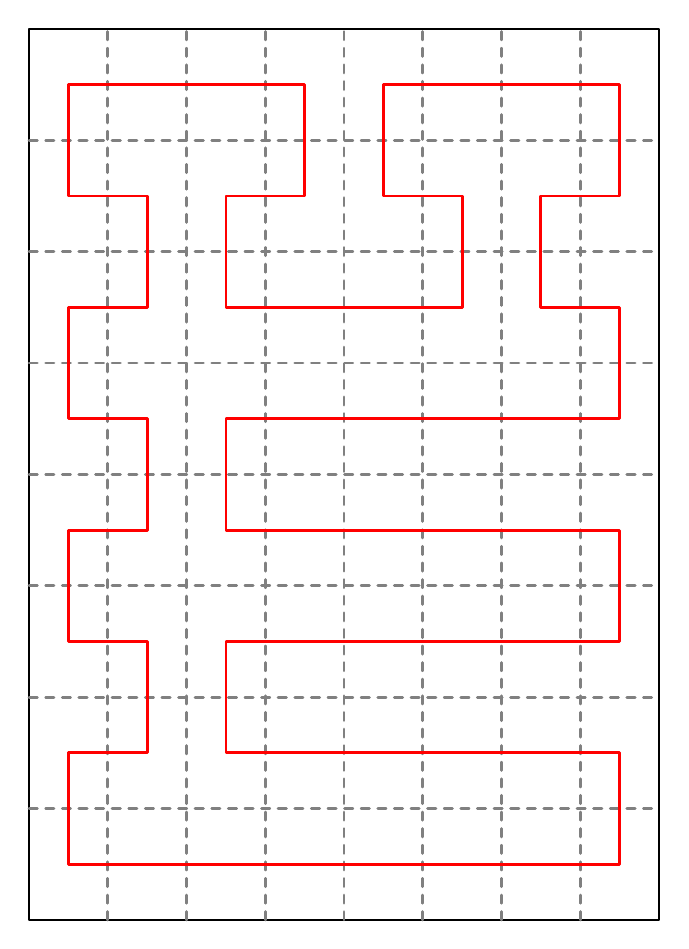
\begin{tikzpicture}[x=1.0cm,y=1.4142135623730951cm,line width=1pt,line cap=round,line join=round]
\draw (0,0) rectangle (8,8);
\draw[dashed,gray] (1,0) -- (1,8) (2,0) -- (2,8) (3,0) -- (3,8) (4,0) -- (4,8) (5,0) -- (5,8) (6,0) -- (6,8) (7,0) -- (7,8) (0,1) -- (8,1) (0,2) -- (8,2) (0,3) -- (8,3) (0,4) -- (8,4) (0,5) -- (8,5) (0,6) -- (8,6) (0,7) -- (8,7);
\draw[red] (0.5,0.5) -- (1.5,0.5) -- (2.5,0.5) -- (3.5,0.5) -- (4.5,0.5) -- (5.5,0.5) -- (6.5,0.5) -- (7.5,0.5) -- (7.5,1.5) -- (6.5,1.5) -- (5.5,1.5) -- (4.5,1.5) -- (3.5,1.5) -- (2.5,1.5) -- (2.5,2.5) -- (3.5,2.5) -- (4.5,2.5) -- (5.5,2.5) -- (6.5,2.5) -- (7.5,2.5) -- (7.5,3.5) -- (6.5,3.5) -- (5.5,3.5) -- (4.5,3.5) -- (3.5,3.5) -- (2.5,3.5) -- (2.5,4.5) -- (3.5,4.5) -- (4.5,4.5) -- (5.5,4.5) -- (6.5,4.5) -- (7.5,4.5) -- (7.5,5.5) -- (6.5,5.5) -- (6.5,6.5) -- (7.5,6.5) -- (7.5,7.5) -- (6.5,7.5) -- (5.5,7.5) -- (4.5,7.5) -- (4.5,6.5) -- (5.5,6.5) -- (5.5,5.5) -- (4.5,5.5) -- (3.5,5.5) -- (2.5,5.5) -- (2.5,6.5) -- (3.5,6.5) -- (3.5,7.5) -- (2.5,7.5) -- (1.5,7.5) -- (0.5,7.5) -- (0.5,6.5) -- (1.5,6.5) -- (1.5,5.5) -- (0.5,5.5) -- (0.5,4.5) -- (1.5,4.5) -- (1.5,3.5) -- (0.5,3.5) -- (0.5,2.5) -- (1.5,2.5) -- (1.5,1.5) -- (0.5,1.5) -- (0.5,0.5) -- cycle;\end{tikzpicture}

\vspace{5mm}

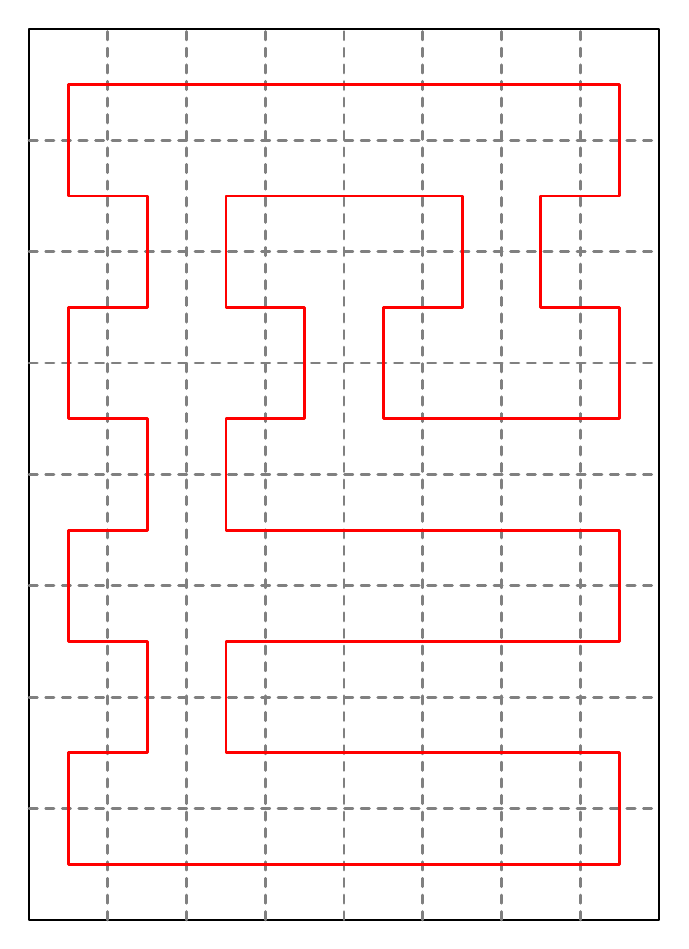
\begin{tikzpicture}[x=1.0cm,y=1.4142135623730951cm,line width=1pt,line cap=round,line join=round]
\draw (0,0) rectangle (8,8);
\draw[dashed,gray] (1,0) -- (1,8) (2,0) -- (2,8) (3,0) -- (3,8) (4,0) -- (4,8) (5,0) -- (5,8) (6,0) -- (6,8) (7,0) -- (7,8) (0,1) -- (8,1) (0,2) -- (8,2) (0,3) -- (8,3) (0,4) -- (8,4) (0,5) -- (8,5) (0,6) -- (8,6) (0,7) -- (8,7);
\draw[red] (0.5,0.5) -- (1.5,0.5) -- (2.5,0.5) -- (3.5,0.5) -- (4.5,0.5) -- (5.5,0.5) -- (6.5,0.5) -- (7.5,0.5) -- (7.5,1.5) -- (6.5,1.5) -- (5.5,1.5) -- (4.5,1.5) -- (3.5,1.5) -- (2.5,1.5) -- (2.5,2.5) -- (3.5,2.5) -- (4.5,2.5) -- (5.5,2.5) -- (6.5,2.5) -- (7.5,2.5) -- (7.5,3.5) -- (6.5,3.5) -- (5.5,3.5) -- (4.5,3.5) -- (3.5,3.5) -- (2.5,3.5) -- (2.5,4.5) -- (3.5,4.5) -- (3.5,5.5) -- (2.5,5.5) -- (2.5,6.5) -- (3.5,6.5) -- (4.5,6.5) -- (5.5,6.5) -- (5.5,5.5) -- (4.5,5.5) -- (4.5,4.5) -- (5.5,4.5) -- (6.5,4.5) -- (7.5,4.5) -- (7.5,5.5) -- (6.5,5.5) -- (6.5,6.5) -- (7.5,6.5) -- (7.5,7.5) -- (6.5,7.5) -- (5.5,7.5) -- (4.5,7.5) -- (3.5,7.5) -- (2.5,7.5) -- (1.5,7.5) -- (0.5,7.5) -- (0.5,6.5) -- (1.5,6.5) -- (1.5,5.5) -- (0.5,5.5) -- (0.5,4.5) -- (1.5,4.5) -- (1.5,3.5) -- (0.5,3.5) -- (0.5,2.5) -- (1.5,2.5) -- (1.5,1.5) -- (0.5,1.5) -- (0.5,0.5) -- cycle;\end{tikzpicture}
\hspace{5mm}
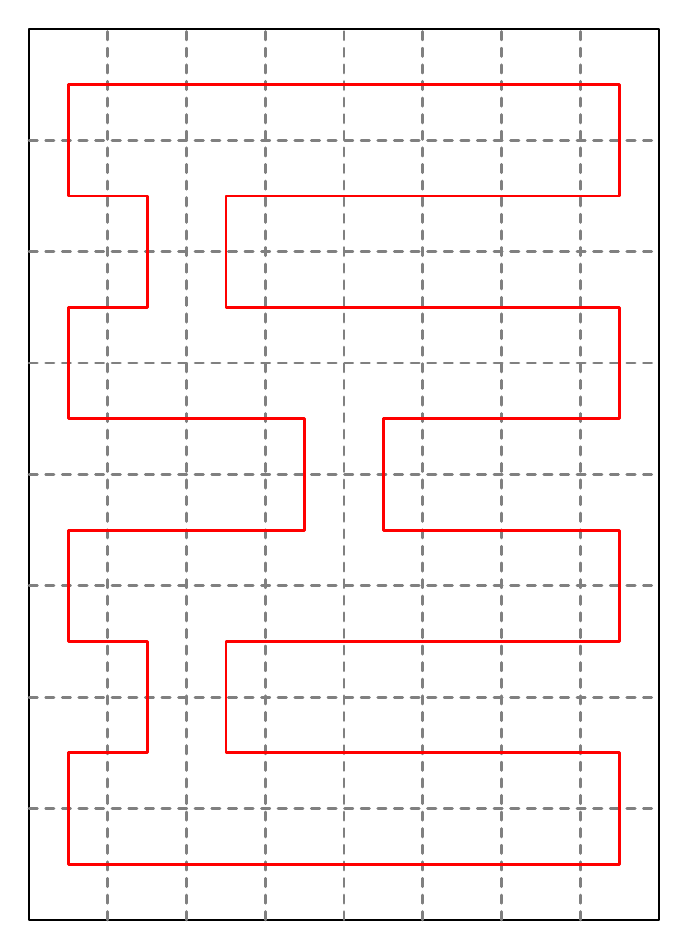
\begin{tikzpicture}[x=1.0cm,y=1.4142135623730951cm,line width=1pt,line cap=round,line join=round]
\draw (0,0) rectangle (8,8);
\draw[dashed,gray] (1,0) -- (1,8) (2,0) -- (2,8) (3,0) -- (3,8) (4,0) -- (4,8) (5,0) -- (5,8) (6,0) -- (6,8) (7,0) -- (7,8) (0,1) -- (8,1) (0,2) -- (8,2) (0,3) -- (8,3) (0,4) -- (8,4) (0,5) -- (8,5) (0,6) -- (8,6) (0,7) -- (8,7);
\draw[red] (0.5,0.5) -- (1.5,0.5) -- (2.5,0.5) -- (3.5,0.5) -- (4.5,0.5) -- (5.5,0.5) -- (6.5,0.5) -- (7.5,0.5) -- (7.5,1.5) -- (6.5,1.5) -- (5.5,1.5) -- (4.5,1.5) -- (3.5,1.5) -- (2.5,1.5) -- (2.5,2.5) -- (3.5,2.5) -- (4.5,2.5) -- (5.5,2.5) -- (6.5,2.5) -- (7.5,2.5) -- (7.5,3.5) -- (6.5,3.5) -- (5.5,3.5) -- (4.5,3.5) -- (4.5,4.5) -- (5.5,4.5) -- (6.5,4.5) -- (7.5,4.5) -- (7.5,5.5) -- (6.5,5.5) -- (5.5,5.5) -- (4.5,5.5) -- (3.5,5.5) -- (2.5,5.5) -- (2.5,6.5) -- (3.5,6.5) -- (4.5,6.5) -- (5.5,6.5) -- (6.5,6.5) -- (7.5,6.5) -- (7.5,7.5) -- (6.5,7.5) -- (5.5,7.5) -- (4.5,7.5) -- (3.5,7.5) -- (2.5,7.5) -- (1.5,7.5) -- (0.5,7.5) -- (0.5,6.5) -- (1.5,6.5) -- (1.5,5.5) -- (0.5,5.5) -- (0.5,4.5) -- (1.5,4.5) -- (2.5,4.5) -- (3.5,4.5) -- (3.5,3.5) -- (2.5,3.5) -- (1.5,3.5) -- (0.5,3.5) -- (0.5,2.5) -- (1.5,2.5) -- (1.5,1.5) -- (0.5,1.5) -- (0.5,0.5) -- cycle;\end{tikzpicture}

\vspace{5mm}

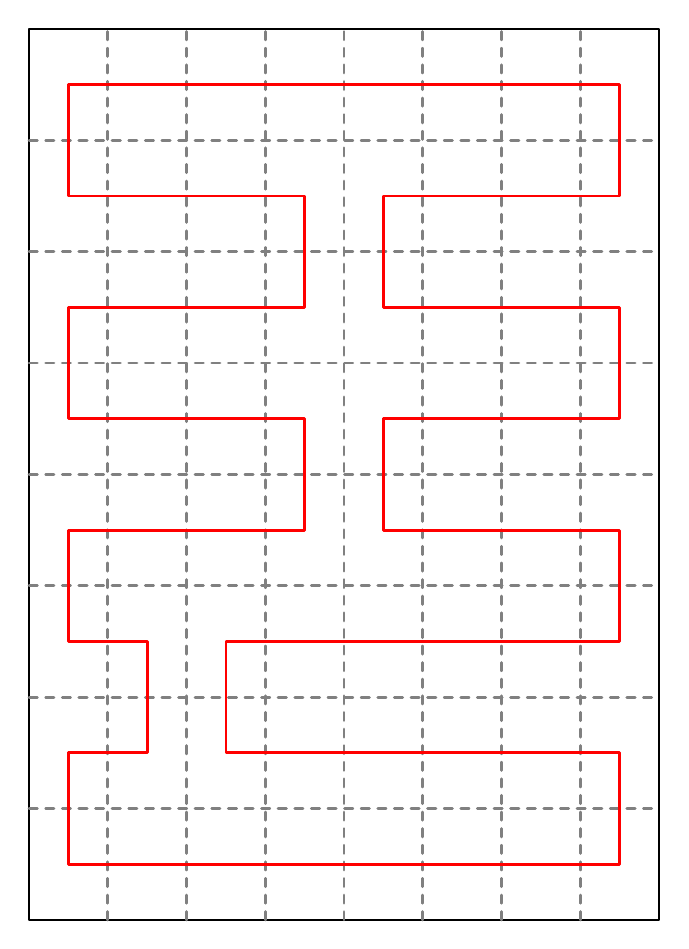
\begin{tikzpicture}[x=1.0cm,y=1.4142135623730951cm,line width=1pt,line cap=round,line join=round]
\draw (0,0) rectangle (8,8);
\draw[dashed,gray] (1,0) -- (1,8) (2,0) -- (2,8) (3,0) -- (3,8) (4,0) -- (4,8) (5,0) -- (5,8) (6,0) -- (6,8) (7,0) -- (7,8) (0,1) -- (8,1) (0,2) -- (8,2) (0,3) -- (8,3) (0,4) -- (8,4) (0,5) -- (8,5) (0,6) -- (8,6) (0,7) -- (8,7);
\draw[red] (0.5,0.5) -- (1.5,0.5) -- (2.5,0.5) -- (3.5,0.5) -- (4.5,0.5) -- (5.5,0.5) -- (6.5,0.5) -- (7.5,0.5) -- (7.5,1.5) -- (6.5,1.5) -- (5.5,1.5) -- (4.5,1.5) -- (3.5,1.5) -- (2.5,1.5) -- (2.5,2.5) -- (3.5,2.5) -- (4.5,2.5) -- (5.5,2.5) -- (6.5,2.5) -- (7.5,2.5) -- (7.5,3.5) -- (6.5,3.5) -- (5.5,3.5) -- (4.5,3.5) -- (4.5,4.5) -- (5.5,4.5) -- (6.5,4.5) -- (7.5,4.5) -- (7.5,5.5) -- (6.5,5.5) -- (5.5,5.5) -- (4.5,5.5) -- (4.5,6.5) -- (5.5,6.5) -- (6.5,6.5) -- (7.5,6.5) -- (7.5,7.5) -- (6.5,7.5) -- (5.5,7.5) -- (4.5,7.5) -- (3.5,7.5) -- (2.5,7.5) -- (1.5,7.5) -- (0.5,7.5) -- (0.5,6.5) -- (1.5,6.5) -- (2.5,6.5) -- (3.5,6.5) -- (3.5,5.5) -- (2.5,5.5) -- (1.5,5.5) -- (0.5,5.5) -- (0.5,4.5) -- (1.5,4.5) -- (2.5,4.5) -- (3.5,4.5) -- (3.5,3.5) -- (2.5,3.5) -- (1.5,3.5) -- (0.5,3.5) -- (0.5,2.5) -- (1.5,2.5) -- (1.5,1.5) -- (0.5,1.5) -- (0.5,0.5) -- cycle;\end{tikzpicture}
\hspace{5mm}
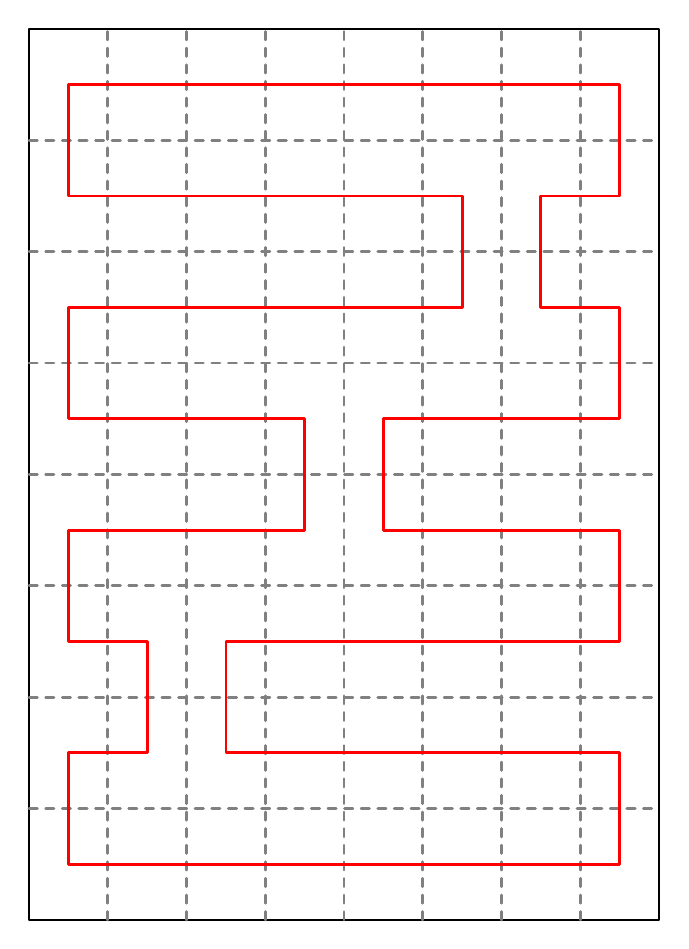
\begin{tikzpicture}[x=1.0cm,y=1.4142135623730951cm,line width=1pt,line cap=round,line join=round]
\draw (0,0) rectangle (8,8);
\draw[dashed,gray] (1,0) -- (1,8) (2,0) -- (2,8) (3,0) -- (3,8) (4,0) -- (4,8) (5,0) -- (5,8) (6,0) -- (6,8) (7,0) -- (7,8) (0,1) -- (8,1) (0,2) -- (8,2) (0,3) -- (8,3) (0,4) -- (8,4) (0,5) -- (8,5) (0,6) -- (8,6) (0,7) -- (8,7);
\draw[red] (0.5,0.5) -- (1.5,0.5) -- (2.5,0.5) -- (3.5,0.5) -- (4.5,0.5) -- (5.5,0.5) -- (6.5,0.5) -- (7.5,0.5) -- (7.5,1.5) -- (6.5,1.5) -- (5.5,1.5) -- (4.5,1.5) -- (3.5,1.5) -- (2.5,1.5) -- (2.5,2.5) -- (3.5,2.5) -- (4.5,2.5) -- (5.5,2.5) -- (6.5,2.5) -- (7.5,2.5) -- (7.5,3.5) -- (6.5,3.5) -- (5.5,3.5) -- (4.5,3.5) -- (4.5,4.5) -- (5.5,4.5) -- (6.5,4.5) -- (7.5,4.5) -- (7.5,5.5) -- (6.5,5.5) -- (6.5,6.5) -- (7.5,6.5) -- (7.5,7.5) -- (6.5,7.5) -- (5.5,7.5) -- (4.5,7.5) -- (3.5,7.5) -- (2.5,7.5) -- (1.5,7.5) -- (0.5,7.5) -- (0.5,6.5) -- (1.5,6.5) -- (2.5,6.5) -- (3.5,6.5) -- (4.5,6.5) -- (5.5,6.5) -- (5.5,5.5) -- (4.5,5.5) -- (3.5,5.5) -- (2.5,5.5) -- (1.5,5.5) -- (0.5,5.5) -- (0.5,4.5) -- (1.5,4.5) -- (2.5,4.5) -- (3.5,4.5) -- (3.5,3.5) -- (2.5,3.5) -- (1.5,3.5) -- (0.5,3.5) -- (0.5,2.5) -- (1.5,2.5) -- (1.5,1.5) -- (0.5,1.5) -- (0.5,0.5) -- cycle;\end{tikzpicture}

\vspace{5mm}

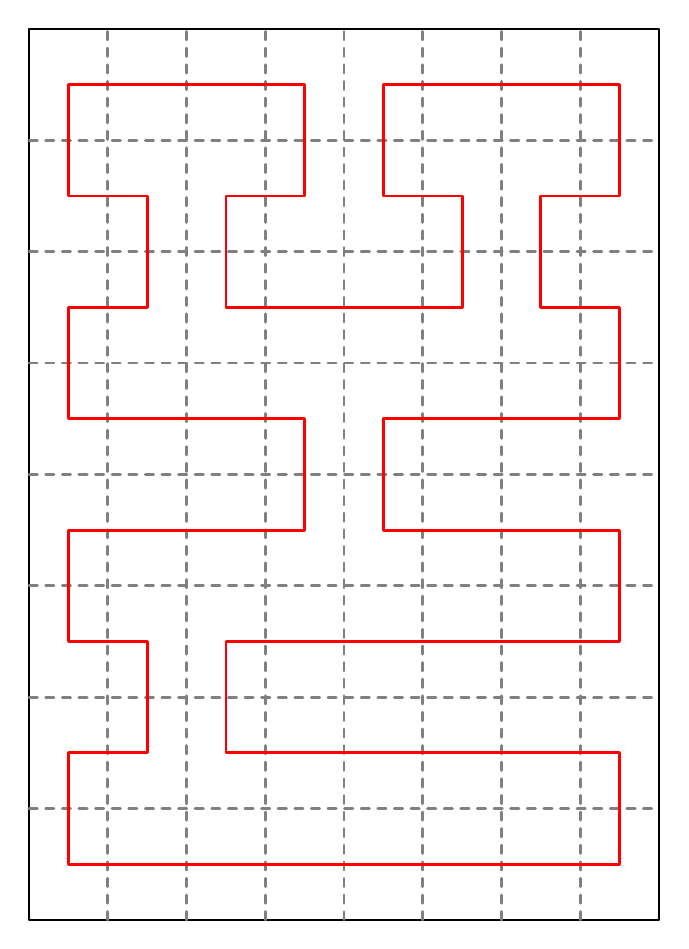
\begin{tikzpicture}[x=1.0cm,y=1.4142135623730951cm,line width=1pt,line cap=round,line join=round]
\draw (0,0) rectangle (8,8);
\draw[dashed,gray] (1,0) -- (1,8) (2,0) -- (2,8) (3,0) -- (3,8) (4,0) -- (4,8) (5,0) -- (5,8) (6,0) -- (6,8) (7,0) -- (7,8) (0,1) -- (8,1) (0,2) -- (8,2) (0,3) -- (8,3) (0,4) -- (8,4) (0,5) -- (8,5) (0,6) -- (8,6) (0,7) -- (8,7);
\draw[red] (0.5,0.5) -- (1.5,0.5) -- (2.5,0.5) -- (3.5,0.5) -- (4.5,0.5) -- (5.5,0.5) -- (6.5,0.5) -- (7.5,0.5) -- (7.5,1.5) -- (6.5,1.5) -- (5.5,1.5) -- (4.5,1.5) -- (3.5,1.5) -- (2.5,1.5) -- (2.5,2.5) -- (3.5,2.5) -- (4.5,2.5) -- (5.5,2.5) -- (6.5,2.5) -- (7.5,2.5) -- (7.5,3.5) -- (6.5,3.5) -- (5.5,3.5) -- (4.5,3.5) -- (4.5,4.5) -- (5.5,4.5) -- (6.5,4.5) -- (7.5,4.5) -- (7.5,5.5) -- (6.5,5.5) -- (6.5,6.5) -- (7.5,6.5) -- (7.5,7.5) -- (6.5,7.5) -- (5.5,7.5) -- (4.5,7.5) -- (4.5,6.5) -- (5.5,6.5) -- (5.5,5.5) -- (4.5,5.5) -- (3.5,5.5) -- (2.5,5.5) -- (2.5,6.5) -- (3.5,6.5) -- (3.5,7.5) -- (2.5,7.5) -- (1.5,7.5) -- (0.5,7.5) -- (0.5,6.5) -- (1.5,6.5) -- (1.5,5.5) -- (0.5,5.5) -- (0.5,4.5) -- (1.5,4.5) -- (2.5,4.5) -- (3.5,4.5) -- (3.5,3.5) -- (2.5,3.5) -- (1.5,3.5) -- (0.5,3.5) -- (0.5,2.5) -- (1.5,2.5) -- (1.5,1.5) -- (0.5,1.5) -- (0.5,0.5) -- cycle;\end{tikzpicture}
\hspace{5mm}
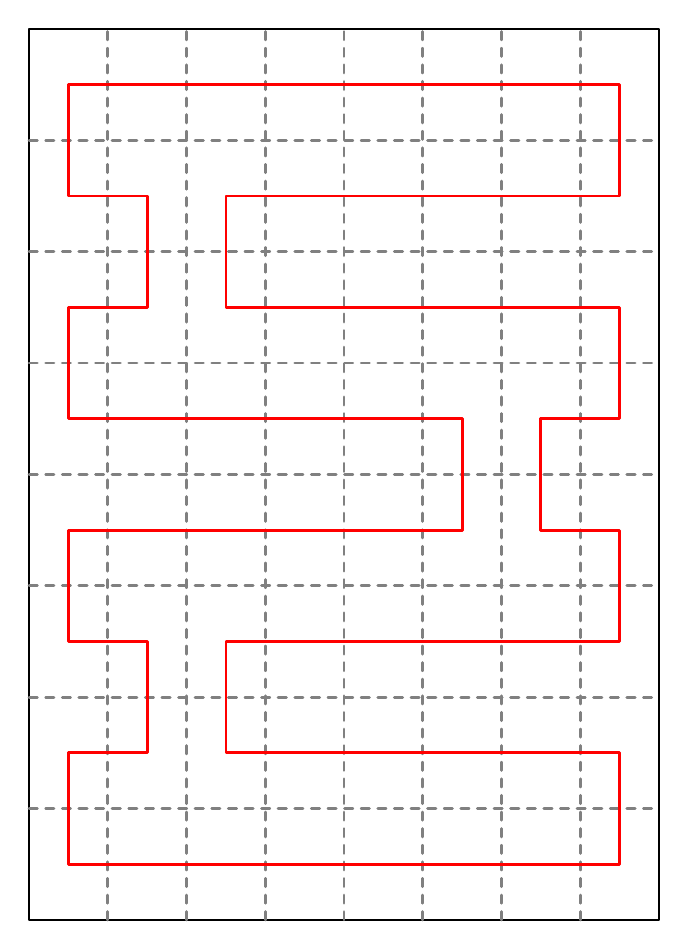
\begin{tikzpicture}[x=1.0cm,y=1.4142135623730951cm,line width=1pt,line cap=round,line join=round]
\draw (0,0) rectangle (8,8);
\draw[dashed,gray] (1,0) -- (1,8) (2,0) -- (2,8) (3,0) -- (3,8) (4,0) -- (4,8) (5,0) -- (5,8) (6,0) -- (6,8) (7,0) -- (7,8) (0,1) -- (8,1) (0,2) -- (8,2) (0,3) -- (8,3) (0,4) -- (8,4) (0,5) -- (8,5) (0,6) -- (8,6) (0,7) -- (8,7);
\draw[red] (0.5,0.5) -- (1.5,0.5) -- (2.5,0.5) -- (3.5,0.5) -- (4.5,0.5) -- (5.5,0.5) -- (6.5,0.5) -- (7.5,0.5) -- (7.5,1.5) -- (6.5,1.5) -- (5.5,1.5) -- (4.5,1.5) -- (3.5,1.5) -- (2.5,1.5) -- (2.5,2.5) -- (3.5,2.5) -- (4.5,2.5) -- (5.5,2.5) -- (6.5,2.5) -- (7.5,2.5) -- (7.5,3.5) -- (6.5,3.5) -- (6.5,4.5) -- (7.5,4.5) -- (7.5,5.5) -- (6.5,5.5) -- (5.5,5.5) -- (4.5,5.5) -- (3.5,5.5) -- (2.5,5.5) -- (2.5,6.5) -- (3.5,6.5) -- (4.5,6.5) -- (5.5,6.5) -- (6.5,6.5) -- (7.5,6.5) -- (7.5,7.5) -- (6.5,7.5) -- (5.5,7.5) -- (4.5,7.5) -- (3.5,7.5) -- (2.5,7.5) -- (1.5,7.5) -- (0.5,7.5) -- (0.5,6.5) -- (1.5,6.5) -- (1.5,5.5) -- (0.5,5.5) -- (0.5,4.5) -- (1.5,4.5) -- (2.5,4.5) -- (3.5,4.5) -- (4.5,4.5) -- (5.5,4.5) -- (5.5,3.5) -- (4.5,3.5) -- (3.5,3.5) -- (2.5,3.5) -- (1.5,3.5) -- (0.5,3.5) -- (0.5,2.5) -- (1.5,2.5) -- (1.5,1.5) -- (0.5,1.5) -- (0.5,0.5) -- cycle;\end{tikzpicture}

\vspace{5mm}

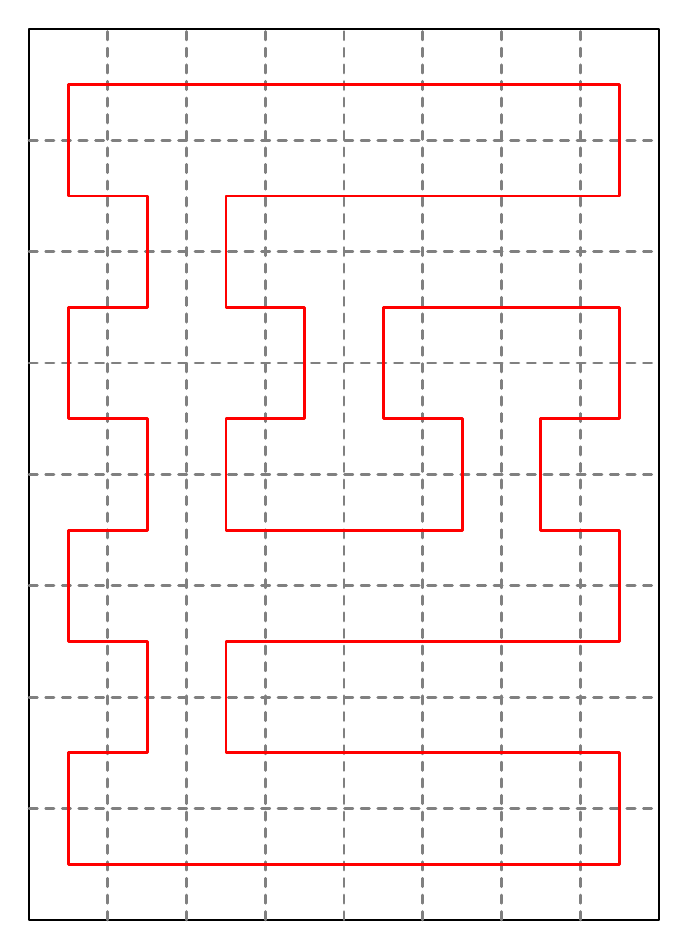
\begin{tikzpicture}[x=1.0cm,y=1.4142135623730951cm,line width=1pt,line cap=round,line join=round]
\draw (0,0) rectangle (8,8);
\draw[dashed,gray] (1,0) -- (1,8) (2,0) -- (2,8) (3,0) -- (3,8) (4,0) -- (4,8) (5,0) -- (5,8) (6,0) -- (6,8) (7,0) -- (7,8) (0,1) -- (8,1) (0,2) -- (8,2) (0,3) -- (8,3) (0,4) -- (8,4) (0,5) -- (8,5) (0,6) -- (8,6) (0,7) -- (8,7);
\draw[red] (0.5,0.5) -- (1.5,0.5) -- (2.5,0.5) -- (3.5,0.5) -- (4.5,0.5) -- (5.5,0.5) -- (6.5,0.5) -- (7.5,0.5) -- (7.5,1.5) -- (6.5,1.5) -- (5.5,1.5) -- (4.5,1.5) -- (3.5,1.5) -- (2.5,1.5) -- (2.5,2.5) -- (3.5,2.5) -- (4.5,2.5) -- (5.5,2.5) -- (6.5,2.5) -- (7.5,2.5) -- (7.5,3.5) -- (6.5,3.5) -- (6.5,4.5) -- (7.5,4.5) -- (7.5,5.5) -- (6.5,5.5) -- (5.5,5.5) -- (4.5,5.5) -- (4.5,4.5) -- (5.5,4.5) -- (5.5,3.5) -- (4.5,3.5) -- (3.5,3.5) -- (2.5,3.5) -- (2.5,4.5) -- (3.5,4.5) -- (3.5,5.5) -- (2.5,5.5) -- (2.5,6.5) -- (3.5,6.5) -- (4.5,6.5) -- (5.5,6.5) -- (6.5,6.5) -- (7.5,6.5) -- (7.5,7.5) -- (6.5,7.5) -- (5.5,7.5) -- (4.5,7.5) -- (3.5,7.5) -- (2.5,7.5) -- (1.5,7.5) -- (0.5,7.5) -- (0.5,6.5) -- (1.5,6.5) -- (1.5,5.5) -- (0.5,5.5) -- (0.5,4.5) -- (1.5,4.5) -- (1.5,3.5) -- (0.5,3.5) -- (0.5,2.5) -- (1.5,2.5) -- (1.5,1.5) -- (0.5,1.5) -- (0.5,0.5) -- cycle;\end{tikzpicture}
\hspace{5mm}
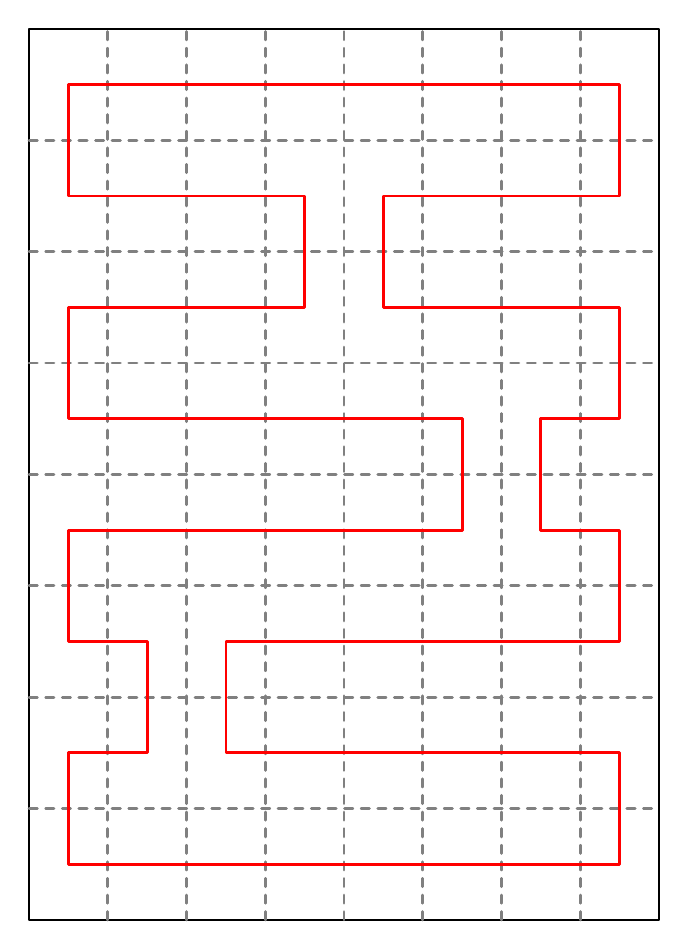
\begin{tikzpicture}[x=1.0cm,y=1.4142135623730951cm,line width=1pt,line cap=round,line join=round]
\draw (0,0) rectangle (8,8);
\draw[dashed,gray] (1,0) -- (1,8) (2,0) -- (2,8) (3,0) -- (3,8) (4,0) -- (4,8) (5,0) -- (5,8) (6,0) -- (6,8) (7,0) -- (7,8) (0,1) -- (8,1) (0,2) -- (8,2) (0,3) -- (8,3) (0,4) -- (8,4) (0,5) -- (8,5) (0,6) -- (8,6) (0,7) -- (8,7);
\draw[red] (0.5,0.5) -- (1.5,0.5) -- (2.5,0.5) -- (3.5,0.5) -- (4.5,0.5) -- (5.5,0.5) -- (6.5,0.5) -- (7.5,0.5) -- (7.5,1.5) -- (6.5,1.5) -- (5.5,1.5) -- (4.5,1.5) -- (3.5,1.5) -- (2.5,1.5) -- (2.5,2.5) -- (3.5,2.5) -- (4.5,2.5) -- (5.5,2.5) -- (6.5,2.5) -- (7.5,2.5) -- (7.5,3.5) -- (6.5,3.5) -- (6.5,4.5) -- (7.5,4.5) -- (7.5,5.5) -- (6.5,5.5) -- (5.5,5.5) -- (4.5,5.5) -- (4.5,6.5) -- (5.5,6.5) -- (6.5,6.5) -- (7.5,6.5) -- (7.5,7.5) -- (6.5,7.5) -- (5.5,7.5) -- (4.5,7.5) -- (3.5,7.5) -- (2.5,7.5) -- (1.5,7.5) -- (0.5,7.5) -- (0.5,6.5) -- (1.5,6.5) -- (2.5,6.5) -- (3.5,6.5) -- (3.5,5.5) -- (2.5,5.5) -- (1.5,5.5) -- (0.5,5.5) -- (0.5,4.5) -- (1.5,4.5) -- (2.5,4.5) -- (3.5,4.5) -- (4.5,4.5) -- (5.5,4.5) -- (5.5,3.5) -- (4.5,3.5) -- (3.5,3.5) -- (2.5,3.5) -- (1.5,3.5) -- (0.5,3.5) -- (0.5,2.5) -- (1.5,2.5) -- (1.5,1.5) -- (0.5,1.5) -- (0.5,0.5) -- cycle;\end{tikzpicture}

\vspace{5mm}

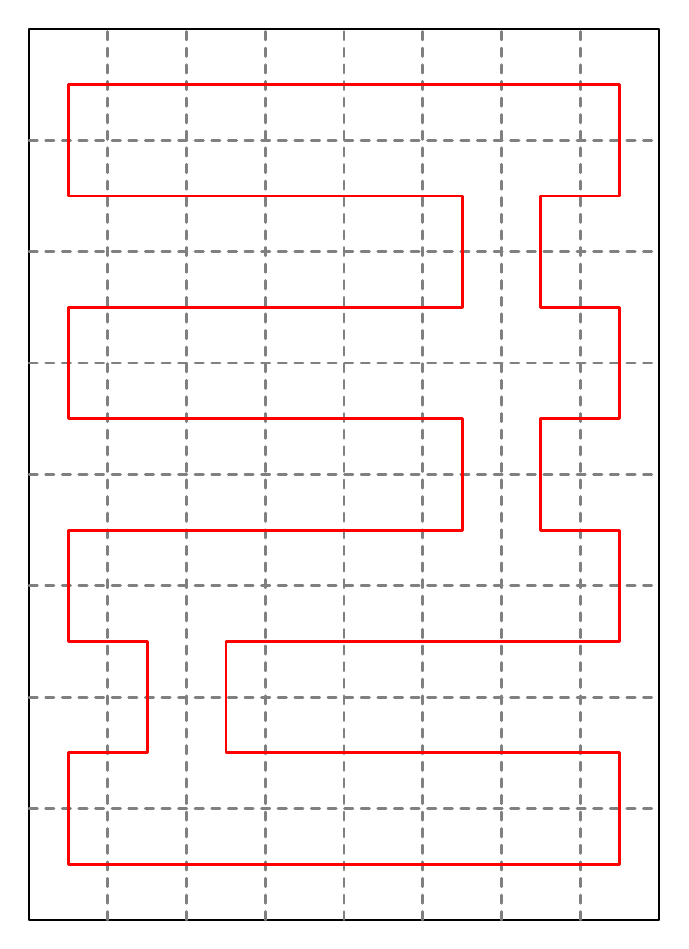
\begin{tikzpicture}[x=1.0cm,y=1.4142135623730951cm,line width=1pt,line cap=round,line join=round]
\draw (0,0) rectangle (8,8);
\draw[dashed,gray] (1,0) -- (1,8) (2,0) -- (2,8) (3,0) -- (3,8) (4,0) -- (4,8) (5,0) -- (5,8) (6,0) -- (6,8) (7,0) -- (7,8) (0,1) -- (8,1) (0,2) -- (8,2) (0,3) -- (8,3) (0,4) -- (8,4) (0,5) -- (8,5) (0,6) -- (8,6) (0,7) -- (8,7);
\draw[red] (0.5,0.5) -- (1.5,0.5) -- (2.5,0.5) -- (3.5,0.5) -- (4.5,0.5) -- (5.5,0.5) -- (6.5,0.5) -- (7.5,0.5) -- (7.5,1.5) -- (6.5,1.5) -- (5.5,1.5) -- (4.5,1.5) -- (3.5,1.5) -- (2.5,1.5) -- (2.5,2.5) -- (3.5,2.5) -- (4.5,2.5) -- (5.5,2.5) -- (6.5,2.5) -- (7.5,2.5) -- (7.5,3.5) -- (6.5,3.5) -- (6.5,4.5) -- (7.5,4.5) -- (7.5,5.5) -- (6.5,5.5) -- (6.5,6.5) -- (7.5,6.5) -- (7.5,7.5) -- (6.5,7.5) -- (5.5,7.5) -- (4.5,7.5) -- (3.5,7.5) -- (2.5,7.5) -- (1.5,7.5) -- (0.5,7.5) -- (0.5,6.5) -- (1.5,6.5) -- (2.5,6.5) -- (3.5,6.5) -- (4.5,6.5) -- (5.5,6.5) -- (5.5,5.5) -- (4.5,5.5) -- (3.5,5.5) -- (2.5,5.5) -- (1.5,5.5) -- (0.5,5.5) -- (0.5,4.5) -- (1.5,4.5) -- (2.5,4.5) -- (3.5,4.5) -- (4.5,4.5) -- (5.5,4.5) -- (5.5,3.5) -- (4.5,3.5) -- (3.5,3.5) -- (2.5,3.5) -- (1.5,3.5) -- (0.5,3.5) -- (0.5,2.5) -- (1.5,2.5) -- (1.5,1.5) -- (0.5,1.5) -- (0.5,0.5) -- cycle;\end{tikzpicture}
\hspace{5mm}
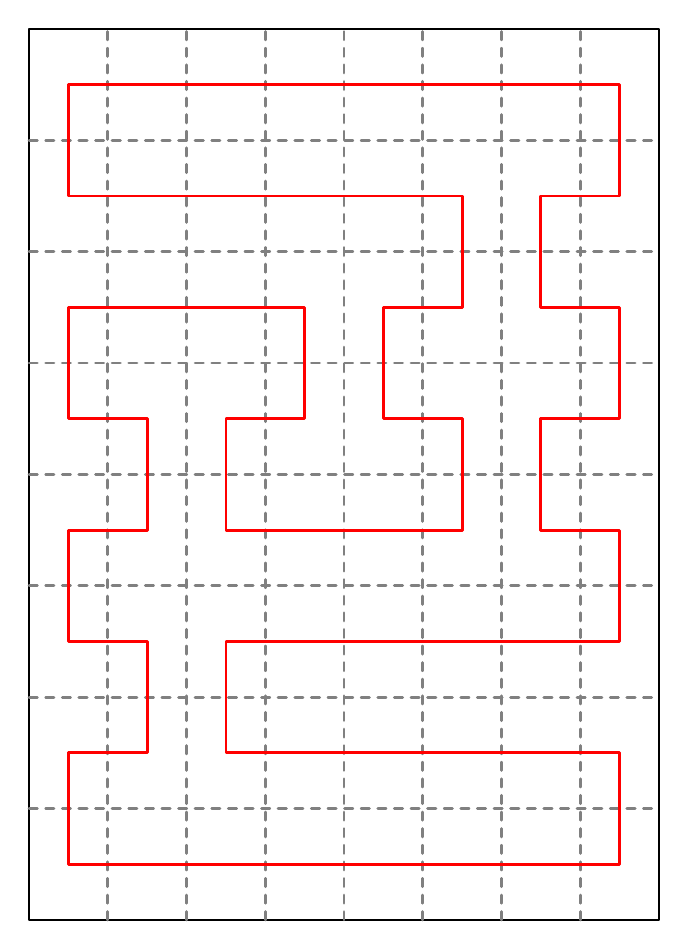
\begin{tikzpicture}[x=1.0cm,y=1.4142135623730951cm,line width=1pt,line cap=round,line join=round]
\draw (0,0) rectangle (8,8);
\draw[dashed,gray] (1,0) -- (1,8) (2,0) -- (2,8) (3,0) -- (3,8) (4,0) -- (4,8) (5,0) -- (5,8) (6,0) -- (6,8) (7,0) -- (7,8) (0,1) -- (8,1) (0,2) -- (8,2) (0,3) -- (8,3) (0,4) -- (8,4) (0,5) -- (8,5) (0,6) -- (8,6) (0,7) -- (8,7);
\draw[red] (0.5,0.5) -- (1.5,0.5) -- (2.5,0.5) -- (3.5,0.5) -- (4.5,0.5) -- (5.5,0.5) -- (6.5,0.5) -- (7.5,0.5) -- (7.5,1.5) -- (6.5,1.5) -- (5.5,1.5) -- (4.5,1.5) -- (3.5,1.5) -- (2.5,1.5) -- (2.5,2.5) -- (3.5,2.5) -- (4.5,2.5) -- (5.5,2.5) -- (6.5,2.5) -- (7.5,2.5) -- (7.5,3.5) -- (6.5,3.5) -- (6.5,4.5) -- (7.5,4.5) -- (7.5,5.5) -- (6.5,5.5) -- (6.5,6.5) -- (7.5,6.5) -- (7.5,7.5) -- (6.5,7.5) -- (5.5,7.5) -- (4.5,7.5) -- (3.5,7.5) -- (2.5,7.5) -- (1.5,7.5) -- (0.5,7.5) -- (0.5,6.5) -- (1.5,6.5) -- (2.5,6.5) -- (3.5,6.5) -- (4.5,6.5) -- (5.5,6.5) -- (5.5,5.5) -- (4.5,5.5) -- (4.5,4.5) -- (5.5,4.5) -- (5.5,3.5) -- (4.5,3.5) -- (3.5,3.5) -- (2.5,3.5) -- (2.5,4.5) -- (3.5,4.5) -- (3.5,5.5) -- (2.5,5.5) -- (1.5,5.5) -- (0.5,5.5) -- (0.5,4.5) -- (1.5,4.5) -- (1.5,3.5) -- (0.5,3.5) -- (0.5,2.5) -- (1.5,2.5) -- (1.5,1.5) -- (0.5,1.5) -- (0.5,0.5) -- cycle;\end{tikzpicture}

\vspace{5mm}

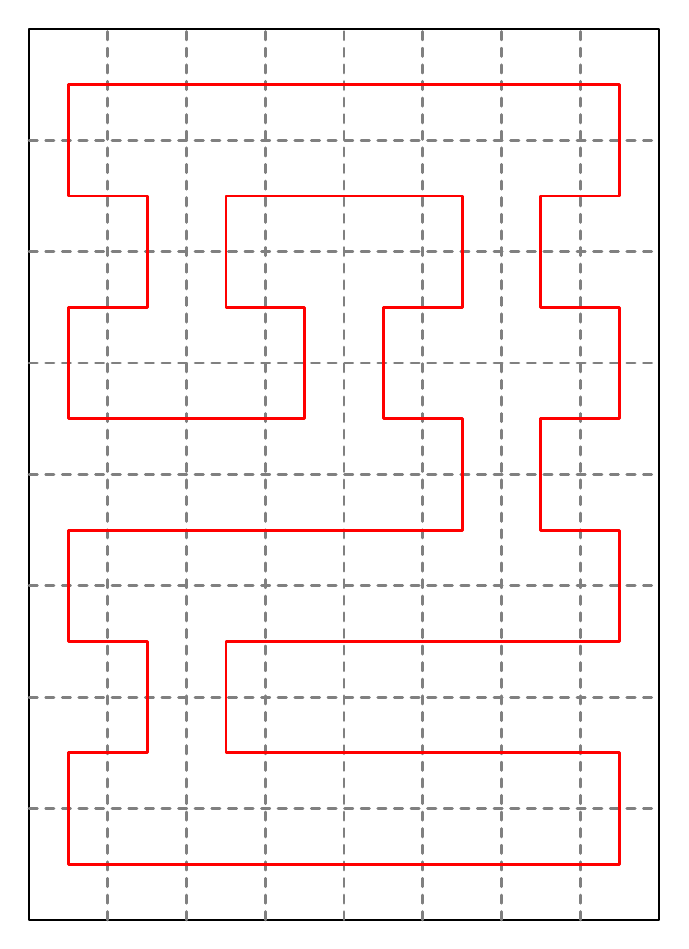
\begin{tikzpicture}[x=1.0cm,y=1.4142135623730951cm,line width=1pt,line cap=round,line join=round]
\draw (0,0) rectangle (8,8);
\draw[dashed,gray] (1,0) -- (1,8) (2,0) -- (2,8) (3,0) -- (3,8) (4,0) -- (4,8) (5,0) -- (5,8) (6,0) -- (6,8) (7,0) -- (7,8) (0,1) -- (8,1) (0,2) -- (8,2) (0,3) -- (8,3) (0,4) -- (8,4) (0,5) -- (8,5) (0,6) -- (8,6) (0,7) -- (8,7);
\draw[red] (0.5,0.5) -- (1.5,0.5) -- (2.5,0.5) -- (3.5,0.5) -- (4.5,0.5) -- (5.5,0.5) -- (6.5,0.5) -- (7.5,0.5) -- (7.5,1.5) -- (6.5,1.5) -- (5.5,1.5) -- (4.5,1.5) -- (3.5,1.5) -- (2.5,1.5) -- (2.5,2.5) -- (3.5,2.5) -- (4.5,2.5) -- (5.5,2.5) -- (6.5,2.5) -- (7.5,2.5) -- (7.5,3.5) -- (6.5,3.5) -- (6.5,4.5) -- (7.5,4.5) -- (7.5,5.5) -- (6.5,5.5) -- (6.5,6.5) -- (7.5,6.5) -- (7.5,7.5) -- (6.5,7.5) -- (5.5,7.5) -- (4.5,7.5) -- (3.5,7.5) -- (2.5,7.5) -- (1.5,7.5) -- (0.5,7.5) -- (0.5,6.5) -- (1.5,6.5) -- (1.5,5.5) -- (0.5,5.5) -- (0.5,4.5) -- (1.5,4.5) -- (2.5,4.5) -- (3.5,4.5) -- (3.5,5.5) -- (2.5,5.5) -- (2.5,6.5) -- (3.5,6.5) -- (4.5,6.5) -- (5.5,6.5) -- (5.5,5.5) -- (4.5,5.5) -- (4.5,4.5) -- (5.5,4.5) -- (5.5,3.5) -- (4.5,3.5) -- (3.5,3.5) -- (2.5,3.5) -- (1.5,3.5) -- (0.5,3.5) -- (0.5,2.5) -- (1.5,2.5) -- (1.5,1.5) -- (0.5,1.5) -- (0.5,0.5) -- cycle;\end{tikzpicture}
\hspace{5mm}
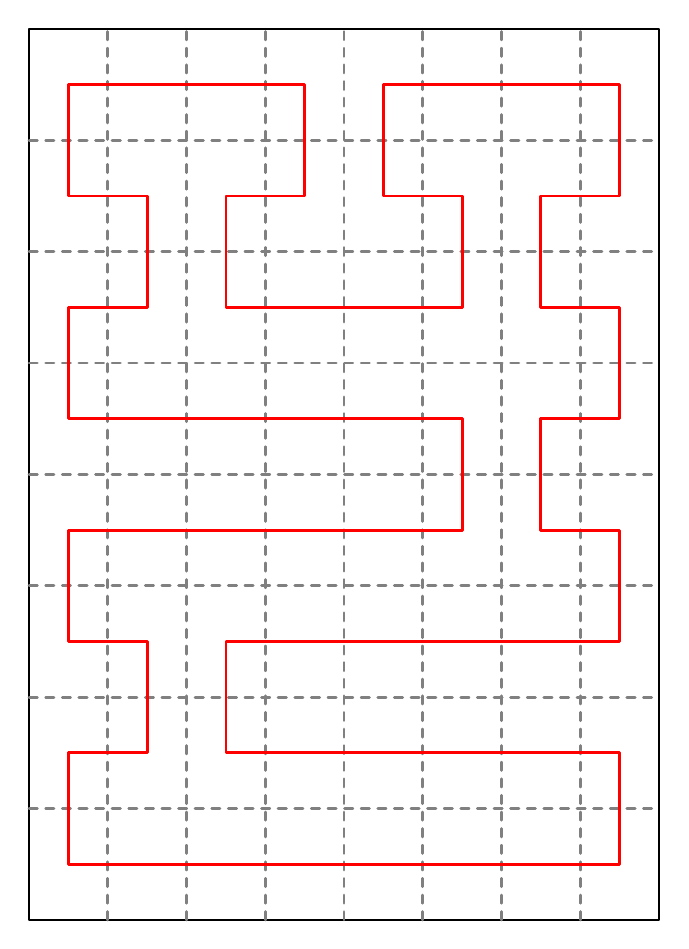
\begin{tikzpicture}[x=1.0cm,y=1.4142135623730951cm,line width=1pt,line cap=round,line join=round]
\draw (0,0) rectangle (8,8);
\draw[dashed,gray] (1,0) -- (1,8) (2,0) -- (2,8) (3,0) -- (3,8) (4,0) -- (4,8) (5,0) -- (5,8) (6,0) -- (6,8) (7,0) -- (7,8) (0,1) -- (8,1) (0,2) -- (8,2) (0,3) -- (8,3) (0,4) -- (8,4) (0,5) -- (8,5) (0,6) -- (8,6) (0,7) -- (8,7);
\draw[red] (0.5,0.5) -- (1.5,0.5) -- (2.5,0.5) -- (3.5,0.5) -- (4.5,0.5) -- (5.5,0.5) -- (6.5,0.5) -- (7.5,0.5) -- (7.5,1.5) -- (6.5,1.5) -- (5.5,1.5) -- (4.5,1.5) -- (3.5,1.5) -- (2.5,1.5) -- (2.5,2.5) -- (3.5,2.5) -- (4.5,2.5) -- (5.5,2.5) -- (6.5,2.5) -- (7.5,2.5) -- (7.5,3.5) -- (6.5,3.5) -- (6.5,4.5) -- (7.5,4.5) -- (7.5,5.5) -- (6.5,5.5) -- (6.5,6.5) -- (7.5,6.5) -- (7.5,7.5) -- (6.5,7.5) -- (5.5,7.5) -- (4.5,7.5) -- (4.5,6.5) -- (5.5,6.5) -- (5.5,5.5) -- (4.5,5.5) -- (3.5,5.5) -- (2.5,5.5) -- (2.5,6.5) -- (3.5,6.5) -- (3.5,7.5) -- (2.5,7.5) -- (1.5,7.5) -- (0.5,7.5) -- (0.5,6.5) -- (1.5,6.5) -- (1.5,5.5) -- (0.5,5.5) -- (0.5,4.5) -- (1.5,4.5) -- (2.5,4.5) -- (3.5,4.5) -- (4.5,4.5) -- (5.5,4.5) -- (5.5,3.5) -- (4.5,3.5) -- (3.5,3.5) -- (2.5,3.5) -- (1.5,3.5) -- (0.5,3.5) -- (0.5,2.5) -- (1.5,2.5) -- (1.5,1.5) -- (0.5,1.5) -- (0.5,0.5) -- cycle;\end{tikzpicture}

\vspace{5mm}

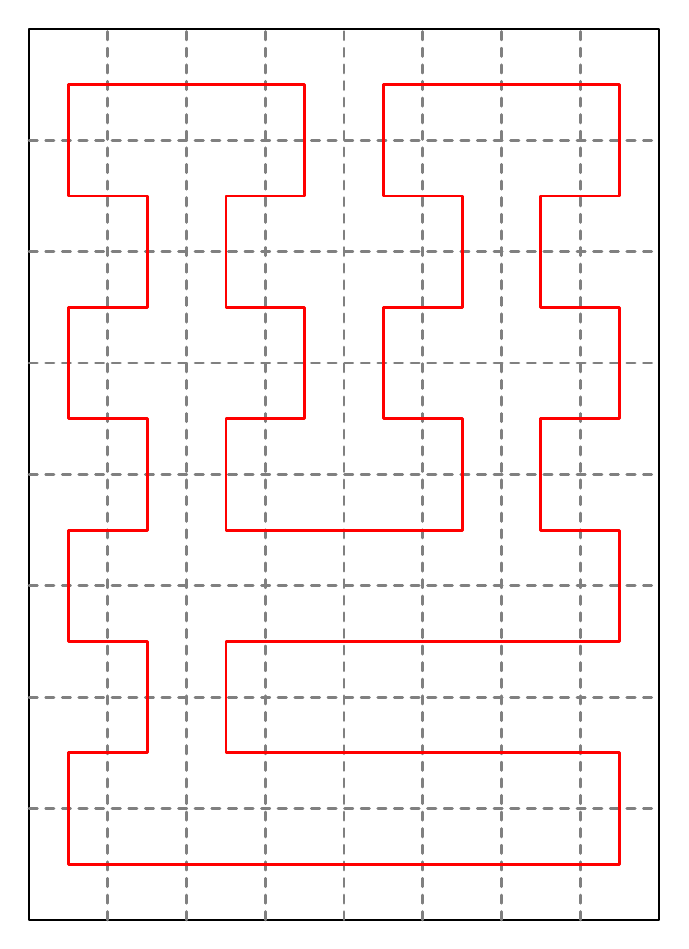
\begin{tikzpicture}[x=1.0cm,y=1.4142135623730951cm,line width=1pt,line cap=round,line join=round]
\draw (0,0) rectangle (8,8);
\draw[dashed,gray] (1,0) -- (1,8) (2,0) -- (2,8) (3,0) -- (3,8) (4,0) -- (4,8) (5,0) -- (5,8) (6,0) -- (6,8) (7,0) -- (7,8) (0,1) -- (8,1) (0,2) -- (8,2) (0,3) -- (8,3) (0,4) -- (8,4) (0,5) -- (8,5) (0,6) -- (8,6) (0,7) -- (8,7);
\draw[red] (0.5,0.5) -- (1.5,0.5) -- (2.5,0.5) -- (3.5,0.5) -- (4.5,0.5) -- (5.5,0.5) -- (6.5,0.5) -- (7.5,0.5) -- (7.5,1.5) -- (6.5,1.5) -- (5.5,1.5) -- (4.5,1.5) -- (3.5,1.5) -- (2.5,1.5) -- (2.5,2.5) -- (3.5,2.5) -- (4.5,2.5) -- (5.5,2.5) -- (6.5,2.5) -- (7.5,2.5) -- (7.5,3.5) -- (6.5,3.5) -- (6.5,4.5) -- (7.5,4.5) -- (7.5,5.5) -- (6.5,5.5) -- (6.5,6.5) -- (7.5,6.5) -- (7.5,7.5) -- (6.5,7.5) -- (5.5,7.5) -- (4.5,7.5) -- (4.5,6.5) -- (5.5,6.5) -- (5.5,5.5) -- (4.5,5.5) -- (4.5,4.5) -- (5.5,4.5) -- (5.5,3.5) -- (4.5,3.5) -- (3.5,3.5) -- (2.5,3.5) -- (2.5,4.5) -- (3.5,4.5) -- (3.5,5.5) -- (2.5,5.5) -- (2.5,6.5) -- (3.5,6.5) -- (3.5,7.5) -- (2.5,7.5) -- (1.5,7.5) -- (0.5,7.5) -- (0.5,6.5) -- (1.5,6.5) -- (1.5,5.5) -- (0.5,5.5) -- (0.5,4.5) -- (1.5,4.5) -- (1.5,3.5) -- (0.5,3.5) -- (0.5,2.5) -- (1.5,2.5) -- (1.5,1.5) -- (0.5,1.5) -- (0.5,0.5) -- cycle;\end{tikzpicture}
\hspace{5mm}
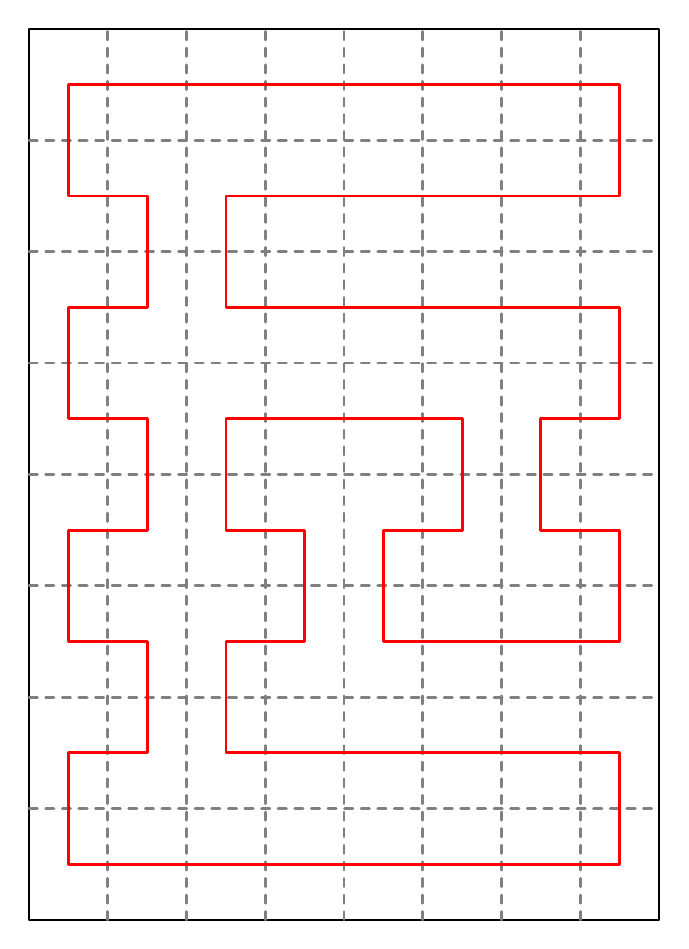
\begin{tikzpicture}[x=1.0cm,y=1.4142135623730951cm,line width=1pt,line cap=round,line join=round]
\draw (0,0) rectangle (8,8);
\draw[dashed,gray] (1,0) -- (1,8) (2,0) -- (2,8) (3,0) -- (3,8) (4,0) -- (4,8) (5,0) -- (5,8) (6,0) -- (6,8) (7,0) -- (7,8) (0,1) -- (8,1) (0,2) -- (8,2) (0,3) -- (8,3) (0,4) -- (8,4) (0,5) -- (8,5) (0,6) -- (8,6) (0,7) -- (8,7);
\draw[red] (0.5,0.5) -- (1.5,0.5) -- (2.5,0.5) -- (3.5,0.5) -- (4.5,0.5) -- (5.5,0.5) -- (6.5,0.5) -- (7.5,0.5) -- (7.5,1.5) -- (6.5,1.5) -- (5.5,1.5) -- (4.5,1.5) -- (3.5,1.5) -- (2.5,1.5) -- (2.5,2.5) -- (3.5,2.5) -- (3.5,3.5) -- (2.5,3.5) -- (2.5,4.5) -- (3.5,4.5) -- (4.5,4.5) -- (5.5,4.5) -- (5.5,3.5) -- (4.5,3.5) -- (4.5,2.5) -- (5.5,2.5) -- (6.5,2.5) -- (7.5,2.5) -- (7.5,3.5) -- (6.5,3.5) -- (6.5,4.5) -- (7.5,4.5) -- (7.5,5.5) -- (6.5,5.5) -- (5.5,5.5) -- (4.5,5.5) -- (3.5,5.5) -- (2.5,5.5) -- (2.5,6.5) -- (3.5,6.5) -- (4.5,6.5) -- (5.5,6.5) -- (6.5,6.5) -- (7.5,6.5) -- (7.5,7.5) -- (6.5,7.5) -- (5.5,7.5) -- (4.5,7.5) -- (3.5,7.5) -- (2.5,7.5) -- (1.5,7.5) -- (0.5,7.5) -- (0.5,6.5) -- (1.5,6.5) -- (1.5,5.5) -- (0.5,5.5) -- (0.5,4.5) -- (1.5,4.5) -- (1.5,3.5) -- (0.5,3.5) -- (0.5,2.5) -- (1.5,2.5) -- (1.5,1.5) -- (0.5,1.5) -- (0.5,0.5) -- cycle;\end{tikzpicture}

\vspace{5mm}

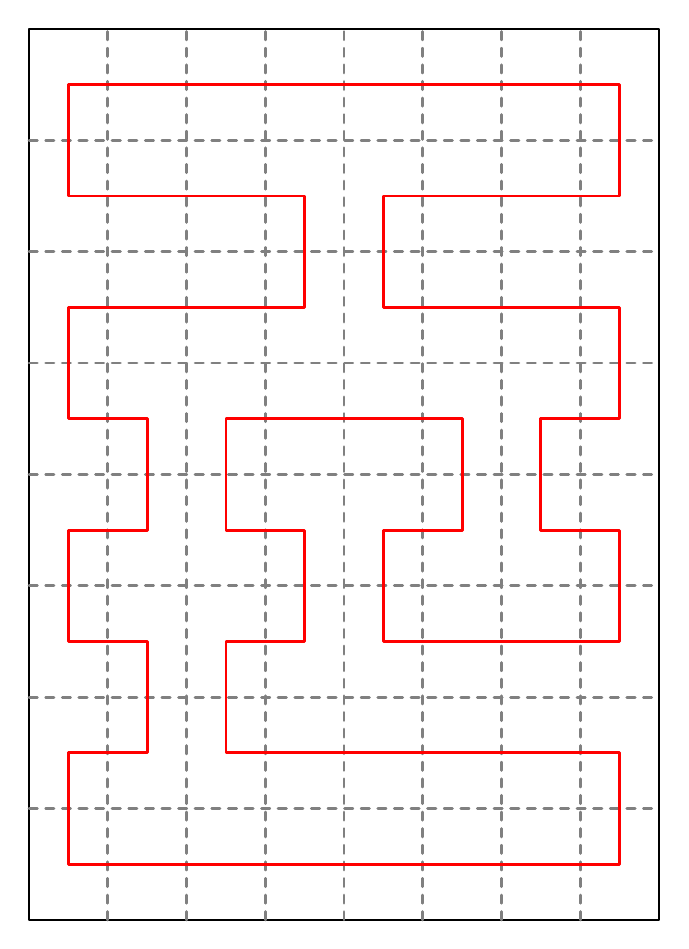
\begin{tikzpicture}[x=1.0cm,y=1.4142135623730951cm,line width=1pt,line cap=round,line join=round]
\draw (0,0) rectangle (8,8);
\draw[dashed,gray] (1,0) -- (1,8) (2,0) -- (2,8) (3,0) -- (3,8) (4,0) -- (4,8) (5,0) -- (5,8) (6,0) -- (6,8) (7,0) -- (7,8) (0,1) -- (8,1) (0,2) -- (8,2) (0,3) -- (8,3) (0,4) -- (8,4) (0,5) -- (8,5) (0,6) -- (8,6) (0,7) -- (8,7);
\draw[red] (0.5,0.5) -- (1.5,0.5) -- (2.5,0.5) -- (3.5,0.5) -- (4.5,0.5) -- (5.5,0.5) -- (6.5,0.5) -- (7.5,0.5) -- (7.5,1.5) -- (6.5,1.5) -- (5.5,1.5) -- (4.5,1.5) -- (3.5,1.5) -- (2.5,1.5) -- (2.5,2.5) -- (3.5,2.5) -- (3.5,3.5) -- (2.5,3.5) -- (2.5,4.5) -- (3.5,4.5) -- (4.5,4.5) -- (5.5,4.5) -- (5.5,3.5) -- (4.5,3.5) -- (4.5,2.5) -- (5.5,2.5) -- (6.5,2.5) -- (7.5,2.5) -- (7.5,3.5) -- (6.5,3.5) -- (6.5,4.5) -- (7.5,4.5) -- (7.5,5.5) -- (6.5,5.5) -- (5.5,5.5) -- (4.5,5.5) -- (4.5,6.5) -- (5.5,6.5) -- (6.5,6.5) -- (7.5,6.5) -- (7.5,7.5) -- (6.5,7.5) -- (5.5,7.5) -- (4.5,7.5) -- (3.5,7.5) -- (2.5,7.5) -- (1.5,7.5) -- (0.5,7.5) -- (0.5,6.5) -- (1.5,6.5) -- (2.5,6.5) -- (3.5,6.5) -- (3.5,5.5) -- (2.5,5.5) -- (1.5,5.5) -- (0.5,5.5) -- (0.5,4.5) -- (1.5,4.5) -- (1.5,3.5) -- (0.5,3.5) -- (0.5,2.5) -- (1.5,2.5) -- (1.5,1.5) -- (0.5,1.5) -- (0.5,0.5) -- cycle;\end{tikzpicture}
\hspace{5mm}
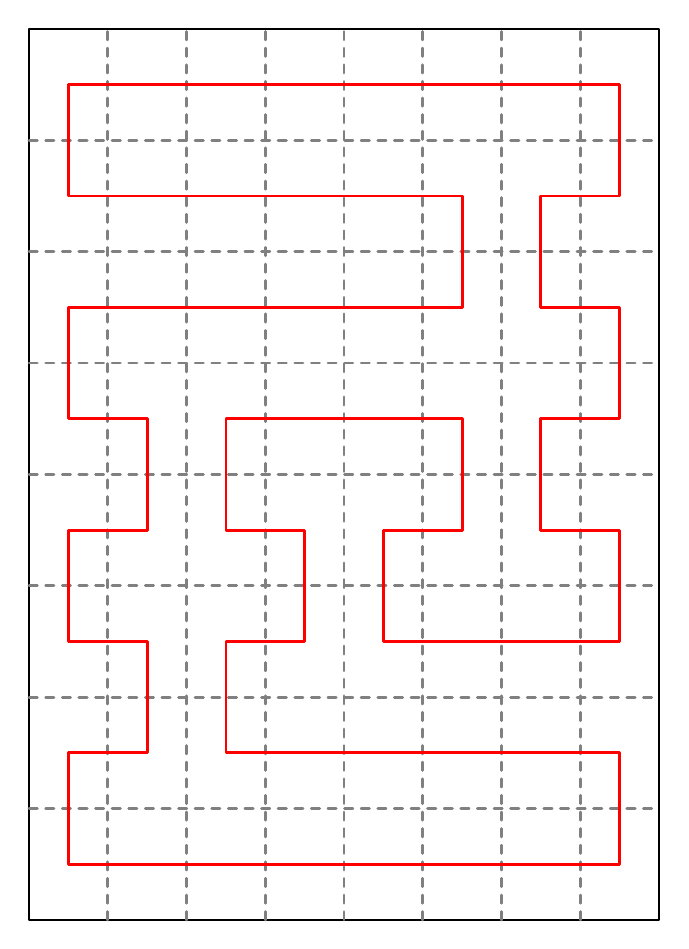
\begin{tikzpicture}[x=1.0cm,y=1.4142135623730951cm,line width=1pt,line cap=round,line join=round]
\draw (0,0) rectangle (8,8);
\draw[dashed,gray] (1,0) -- (1,8) (2,0) -- (2,8) (3,0) -- (3,8) (4,0) -- (4,8) (5,0) -- (5,8) (6,0) -- (6,8) (7,0) -- (7,8) (0,1) -- (8,1) (0,2) -- (8,2) (0,3) -- (8,3) (0,4) -- (8,4) (0,5) -- (8,5) (0,6) -- (8,6) (0,7) -- (8,7);
\draw[red] (0.5,0.5) -- (1.5,0.5) -- (2.5,0.5) -- (3.5,0.5) -- (4.5,0.5) -- (5.5,0.5) -- (6.5,0.5) -- (7.5,0.5) -- (7.5,1.5) -- (6.5,1.5) -- (5.5,1.5) -- (4.5,1.5) -- (3.5,1.5) -- (2.5,1.5) -- (2.5,2.5) -- (3.5,2.5) -- (3.5,3.5) -- (2.5,3.5) -- (2.5,4.5) -- (3.5,4.5) -- (4.5,4.5) -- (5.5,4.5) -- (5.5,3.5) -- (4.5,3.5) -- (4.5,2.5) -- (5.5,2.5) -- (6.5,2.5) -- (7.5,2.5) -- (7.5,3.5) -- (6.5,3.5) -- (6.5,4.5) -- (7.5,4.5) -- (7.5,5.5) -- (6.5,5.5) -- (6.5,6.5) -- (7.5,6.5) -- (7.5,7.5) -- (6.5,7.5) -- (5.5,7.5) -- (4.5,7.5) -- (3.5,7.5) -- (2.5,7.5) -- (1.5,7.5) -- (0.5,7.5) -- (0.5,6.5) -- (1.5,6.5) -- (2.5,6.5) -- (3.5,6.5) -- (4.5,6.5) -- (5.5,6.5) -- (5.5,5.5) -- (4.5,5.5) -- (3.5,5.5) -- (2.5,5.5) -- (1.5,5.5) -- (0.5,5.5) -- (0.5,4.5) -- (1.5,4.5) -- (1.5,3.5) -- (0.5,3.5) -- (0.5,2.5) -- (1.5,2.5) -- (1.5,1.5) -- (0.5,1.5) -- (0.5,0.5) -- cycle;\end{tikzpicture}

\vspace{5mm}

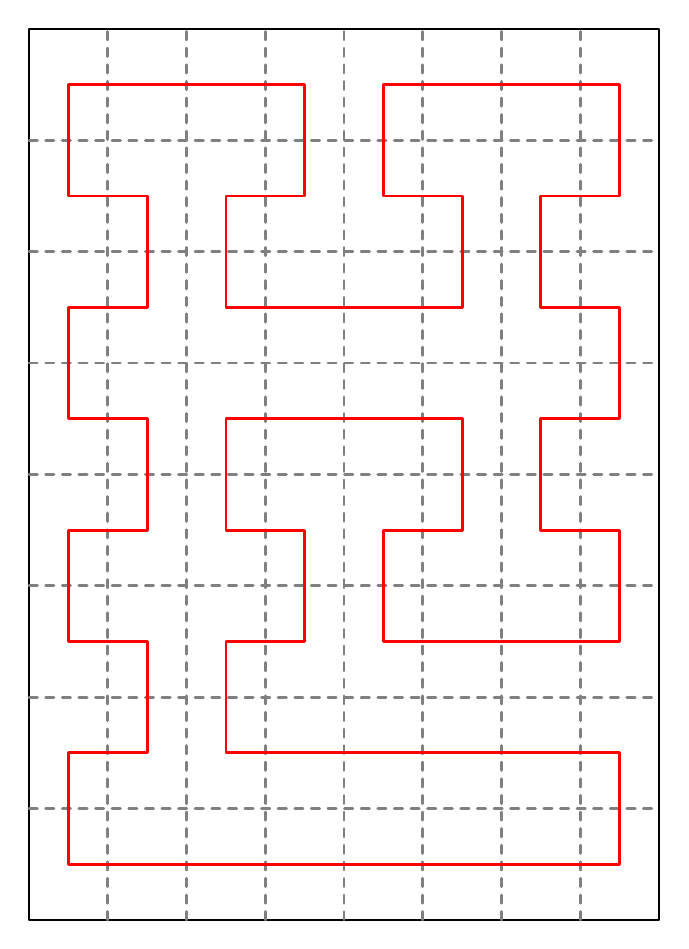
\begin{tikzpicture}[x=1.0cm,y=1.4142135623730951cm,line width=1pt,line cap=round,line join=round]
\draw (0,0) rectangle (8,8);
\draw[dashed,gray] (1,0) -- (1,8) (2,0) -- (2,8) (3,0) -- (3,8) (4,0) -- (4,8) (5,0) -- (5,8) (6,0) -- (6,8) (7,0) -- (7,8) (0,1) -- (8,1) (0,2) -- (8,2) (0,3) -- (8,3) (0,4) -- (8,4) (0,5) -- (8,5) (0,6) -- (8,6) (0,7) -- (8,7);
\draw[red] (0.5,0.5) -- (1.5,0.5) -- (2.5,0.5) -- (3.5,0.5) -- (4.5,0.5) -- (5.5,0.5) -- (6.5,0.5) -- (7.5,0.5) -- (7.5,1.5) -- (6.5,1.5) -- (5.5,1.5) -- (4.5,1.5) -- (3.5,1.5) -- (2.5,1.5) -- (2.5,2.5) -- (3.5,2.5) -- (3.5,3.5) -- (2.5,3.5) -- (2.5,4.5) -- (3.5,4.5) -- (4.5,4.5) -- (5.5,4.5) -- (5.5,3.5) -- (4.5,3.5) -- (4.5,2.5) -- (5.5,2.5) -- (6.5,2.5) -- (7.5,2.5) -- (7.5,3.5) -- (6.5,3.5) -- (6.5,4.5) -- (7.5,4.5) -- (7.5,5.5) -- (6.5,5.5) -- (6.5,6.5) -- (7.5,6.5) -- (7.5,7.5) -- (6.5,7.5) -- (5.5,7.5) -- (4.5,7.5) -- (4.5,6.5) -- (5.5,6.5) -- (5.5,5.5) -- (4.5,5.5) -- (3.5,5.5) -- (2.5,5.5) -- (2.5,6.5) -- (3.5,6.5) -- (3.5,7.5) -- (2.5,7.5) -- (1.5,7.5) -- (0.5,7.5) -- (0.5,6.5) -- (1.5,6.5) -- (1.5,5.5) -- (0.5,5.5) -- (0.5,4.5) -- (1.5,4.5) -- (1.5,3.5) -- (0.5,3.5) -- (0.5,2.5) -- (1.5,2.5) -- (1.5,1.5) -- (0.5,1.5) -- (0.5,0.5) -- cycle;\end{tikzpicture}
\hspace{5mm}
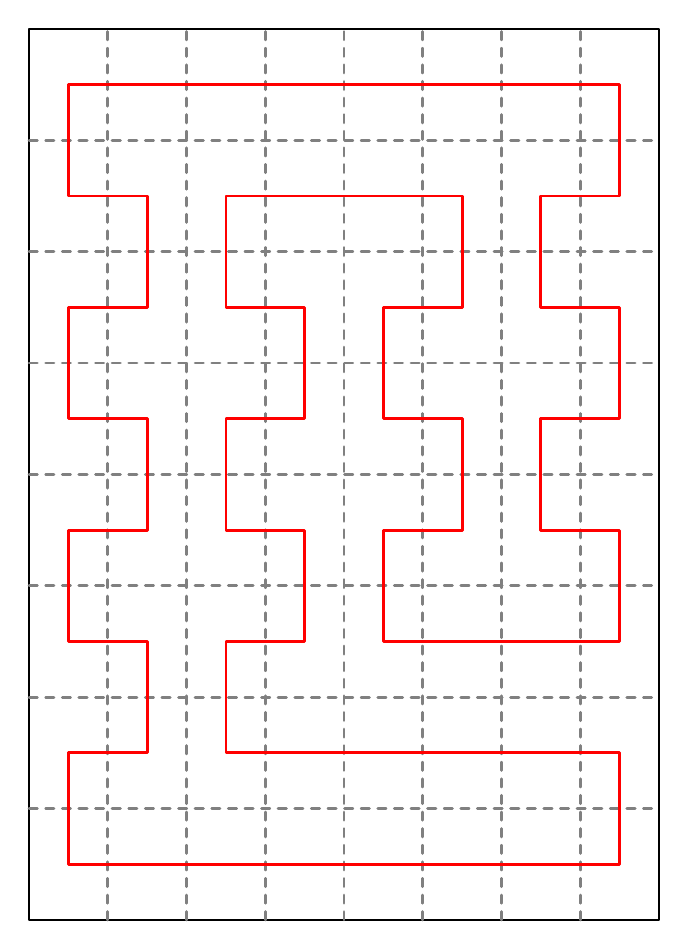
\begin{tikzpicture}[x=1.0cm,y=1.4142135623730951cm,line width=1pt,line cap=round,line join=round]
\draw (0,0) rectangle (8,8);
\draw[dashed,gray] (1,0) -- (1,8) (2,0) -- (2,8) (3,0) -- (3,8) (4,0) -- (4,8) (5,0) -- (5,8) (6,0) -- (6,8) (7,0) -- (7,8) (0,1) -- (8,1) (0,2) -- (8,2) (0,3) -- (8,3) (0,4) -- (8,4) (0,5) -- (8,5) (0,6) -- (8,6) (0,7) -- (8,7);
\draw[red] (0.5,0.5) -- (1.5,0.5) -- (2.5,0.5) -- (3.5,0.5) -- (4.5,0.5) -- (5.5,0.5) -- (6.5,0.5) -- (7.5,0.5) -- (7.5,1.5) -- (6.5,1.5) -- (5.5,1.5) -- (4.5,1.5) -- (3.5,1.5) -- (2.5,1.5) -- (2.5,2.5) -- (3.5,2.5) -- (3.5,3.5) -- (2.5,3.5) -- (2.5,4.5) -- (3.5,4.5) -- (3.5,5.5) -- (2.5,5.5) -- (2.5,6.5) -- (3.5,6.5) -- (4.5,6.5) -- (5.5,6.5) -- (5.5,5.5) -- (4.5,5.5) -- (4.5,4.5) -- (5.5,4.5) -- (5.5,3.5) -- (4.5,3.5) -- (4.5,2.5) -- (5.5,2.5) -- (6.5,2.5) -- (7.5,2.5) -- (7.5,3.5) -- (6.5,3.5) -- (6.5,4.5) -- (7.5,4.5) -- (7.5,5.5) -- (6.5,5.5) -- (6.5,6.5) -- (7.5,6.5) -- (7.5,7.5) -- (6.5,7.5) -- (5.5,7.5) -- (4.5,7.5) -- (3.5,7.5) -- (2.5,7.5) -- (1.5,7.5) -- (0.5,7.5) -- (0.5,6.5) -- (1.5,6.5) -- (1.5,5.5) -- (0.5,5.5) -- (0.5,4.5) -- (1.5,4.5) -- (1.5,3.5) -- (0.5,3.5) -- (0.5,2.5) -- (1.5,2.5) -- (1.5,1.5) -- (0.5,1.5) -- (0.5,0.5) -- cycle;\end{tikzpicture}

\vspace{5mm}

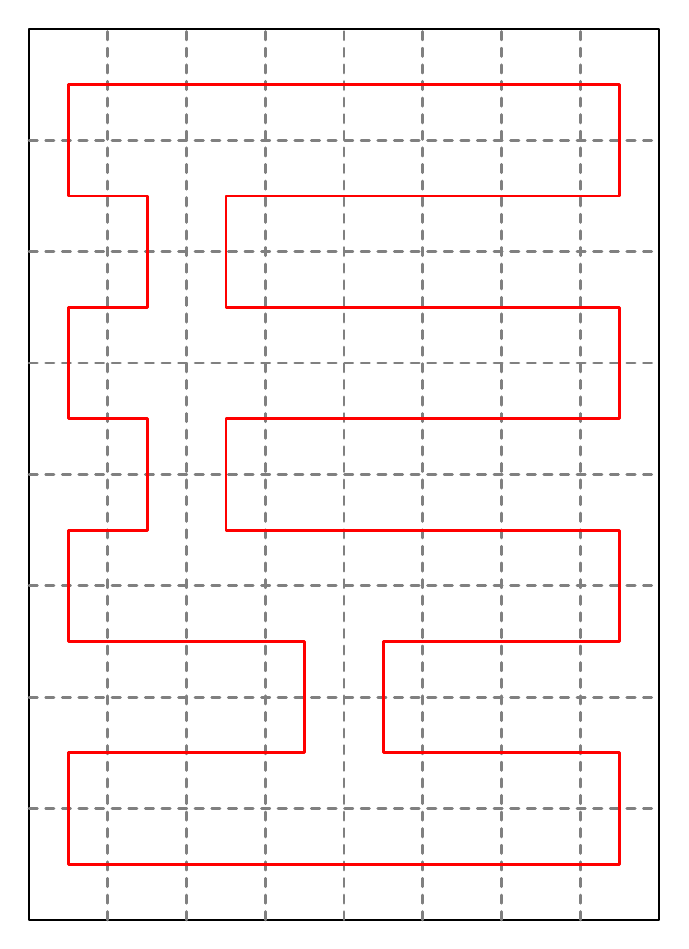
\begin{tikzpicture}[x=1.0cm,y=1.4142135623730951cm,line width=1pt,line cap=round,line join=round]
\draw (0,0) rectangle (8,8);
\draw[dashed,gray] (1,0) -- (1,8) (2,0) -- (2,8) (3,0) -- (3,8) (4,0) -- (4,8) (5,0) -- (5,8) (6,0) -- (6,8) (7,0) -- (7,8) (0,1) -- (8,1) (0,2) -- (8,2) (0,3) -- (8,3) (0,4) -- (8,4) (0,5) -- (8,5) (0,6) -- (8,6) (0,7) -- (8,7);
\draw[red] (0.5,0.5) -- (1.5,0.5) -- (2.5,0.5) -- (3.5,0.5) -- (4.5,0.5) -- (5.5,0.5) -- (6.5,0.5) -- (7.5,0.5) -- (7.5,1.5) -- (6.5,1.5) -- (5.5,1.5) -- (4.5,1.5) -- (4.5,2.5) -- (5.5,2.5) -- (6.5,2.5) -- (7.5,2.5) -- (7.5,3.5) -- (6.5,3.5) -- (5.5,3.5) -- (4.5,3.5) -- (3.5,3.5) -- (2.5,3.5) -- (2.5,4.5) -- (3.5,4.5) -- (4.5,4.5) -- (5.5,4.5) -- (6.5,4.5) -- (7.5,4.5) -- (7.5,5.5) -- (6.5,5.5) -- (5.5,5.5) -- (4.5,5.5) -- (3.5,5.5) -- (2.5,5.5) -- (2.5,6.5) -- (3.5,6.5) -- (4.5,6.5) -- (5.5,6.5) -- (6.5,6.5) -- (7.5,6.5) -- (7.5,7.5) -- (6.5,7.5) -- (5.5,7.5) -- (4.5,7.5) -- (3.5,7.5) -- (2.5,7.5) -- (1.5,7.5) -- (0.5,7.5) -- (0.5,6.5) -- (1.5,6.5) -- (1.5,5.5) -- (0.5,5.5) -- (0.5,4.5) -- (1.5,4.5) -- (1.5,3.5) -- (0.5,3.5) -- (0.5,2.5) -- (1.5,2.5) -- (2.5,2.5) -- (3.5,2.5) -- (3.5,1.5) -- (2.5,1.5) -- (1.5,1.5) -- (0.5,1.5) -- (0.5,0.5) -- cycle;\end{tikzpicture}
\hspace{5mm}
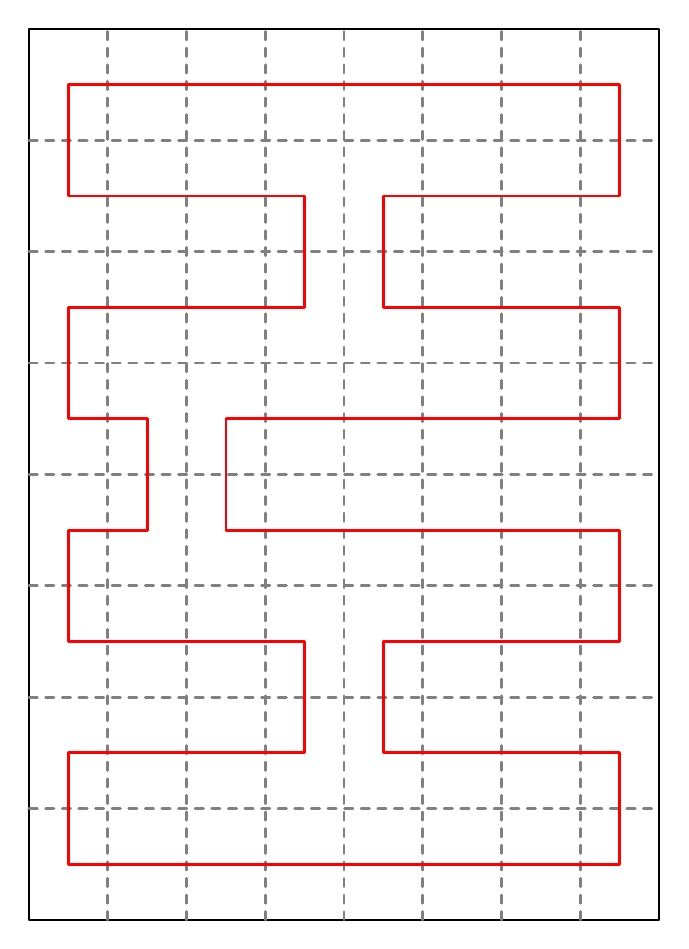
\begin{tikzpicture}[x=1.0cm,y=1.4142135623730951cm,line width=1pt,line cap=round,line join=round]
\draw (0,0) rectangle (8,8);
\draw[dashed,gray] (1,0) -- (1,8) (2,0) -- (2,8) (3,0) -- (3,8) (4,0) -- (4,8) (5,0) -- (5,8) (6,0) -- (6,8) (7,0) -- (7,8) (0,1) -- (8,1) (0,2) -- (8,2) (0,3) -- (8,3) (0,4) -- (8,4) (0,5) -- (8,5) (0,6) -- (8,6) (0,7) -- (8,7);
\draw[red] (0.5,0.5) -- (1.5,0.5) -- (2.5,0.5) -- (3.5,0.5) -- (4.5,0.5) -- (5.5,0.5) -- (6.5,0.5) -- (7.5,0.5) -- (7.5,1.5) -- (6.5,1.5) -- (5.5,1.5) -- (4.5,1.5) -- (4.5,2.5) -- (5.5,2.5) -- (6.5,2.5) -- (7.5,2.5) -- (7.5,3.5) -- (6.5,3.5) -- (5.5,3.5) -- (4.5,3.5) -- (3.5,3.5) -- (2.5,3.5) -- (2.5,4.5) -- (3.5,4.5) -- (4.5,4.5) -- (5.5,4.5) -- (6.5,4.5) -- (7.5,4.5) -- (7.5,5.5) -- (6.5,5.5) -- (5.5,5.5) -- (4.5,5.5) -- (4.5,6.5) -- (5.5,6.5) -- (6.5,6.5) -- (7.5,6.5) -- (7.5,7.5) -- (6.5,7.5) -- (5.5,7.5) -- (4.5,7.5) -- (3.5,7.5) -- (2.5,7.5) -- (1.5,7.5) -- (0.5,7.5) -- (0.5,6.5) -- (1.5,6.5) -- (2.5,6.5) -- (3.5,6.5) -- (3.5,5.5) -- (2.5,5.5) -- (1.5,5.5) -- (0.5,5.5) -- (0.5,4.5) -- (1.5,4.5) -- (1.5,3.5) -- (0.5,3.5) -- (0.5,2.5) -- (1.5,2.5) -- (2.5,2.5) -- (3.5,2.5) -- (3.5,1.5) -- (2.5,1.5) -- (1.5,1.5) -- (0.5,1.5) -- (0.5,0.5) -- cycle;\end{tikzpicture}

\vspace{5mm}

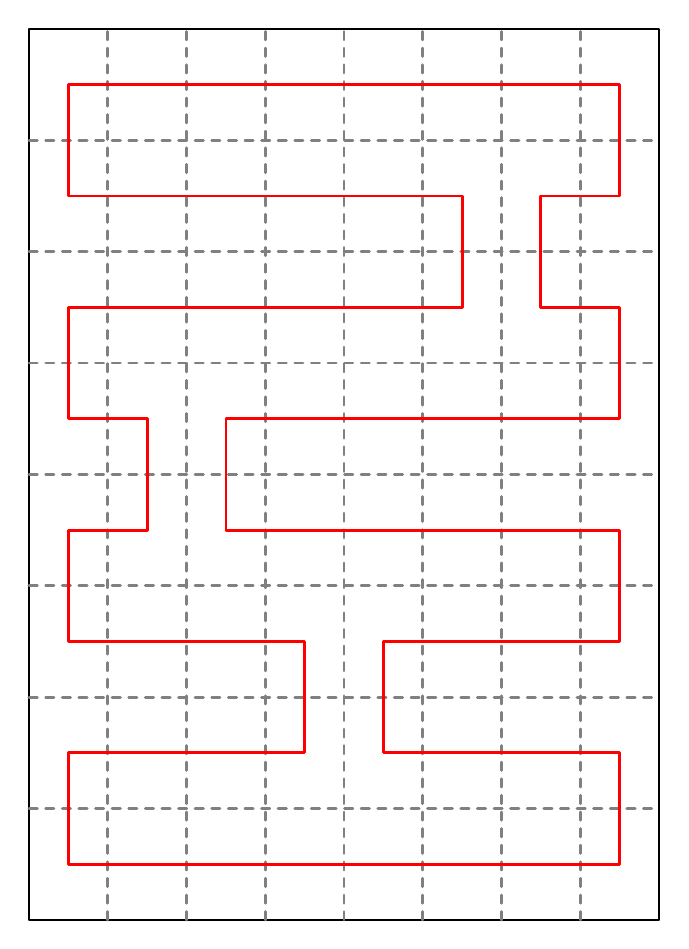
\begin{tikzpicture}[x=1.0cm,y=1.4142135623730951cm,line width=1pt,line cap=round,line join=round]
\draw (0,0) rectangle (8,8);
\draw[dashed,gray] (1,0) -- (1,8) (2,0) -- (2,8) (3,0) -- (3,8) (4,0) -- (4,8) (5,0) -- (5,8) (6,0) -- (6,8) (7,0) -- (7,8) (0,1) -- (8,1) (0,2) -- (8,2) (0,3) -- (8,3) (0,4) -- (8,4) (0,5) -- (8,5) (0,6) -- (8,6) (0,7) -- (8,7);
\draw[red] (0.5,0.5) -- (1.5,0.5) -- (2.5,0.5) -- (3.5,0.5) -- (4.5,0.5) -- (5.5,0.5) -- (6.5,0.5) -- (7.5,0.5) -- (7.5,1.5) -- (6.5,1.5) -- (5.5,1.5) -- (4.5,1.5) -- (4.5,2.5) -- (5.5,2.5) -- (6.5,2.5) -- (7.5,2.5) -- (7.5,3.5) -- (6.5,3.5) -- (5.5,3.5) -- (4.5,3.5) -- (3.5,3.5) -- (2.5,3.5) -- (2.5,4.5) -- (3.5,4.5) -- (4.5,4.5) -- (5.5,4.5) -- (6.5,4.5) -- (7.5,4.5) -- (7.5,5.5) -- (6.5,5.5) -- (6.5,6.5) -- (7.5,6.5) -- (7.5,7.5) -- (6.5,7.5) -- (5.5,7.5) -- (4.5,7.5) -- (3.5,7.5) -- (2.5,7.5) -- (1.5,7.5) -- (0.5,7.5) -- (0.5,6.5) -- (1.5,6.5) -- (2.5,6.5) -- (3.5,6.5) -- (4.5,6.5) -- (5.5,6.5) -- (5.5,5.5) -- (4.5,5.5) -- (3.5,5.5) -- (2.5,5.5) -- (1.5,5.5) -- (0.5,5.5) -- (0.5,4.5) -- (1.5,4.5) -- (1.5,3.5) -- (0.5,3.5) -- (0.5,2.5) -- (1.5,2.5) -- (2.5,2.5) -- (3.5,2.5) -- (3.5,1.5) -- (2.5,1.5) -- (1.5,1.5) -- (0.5,1.5) -- (0.5,0.5) -- cycle;\end{tikzpicture}
\hspace{5mm}
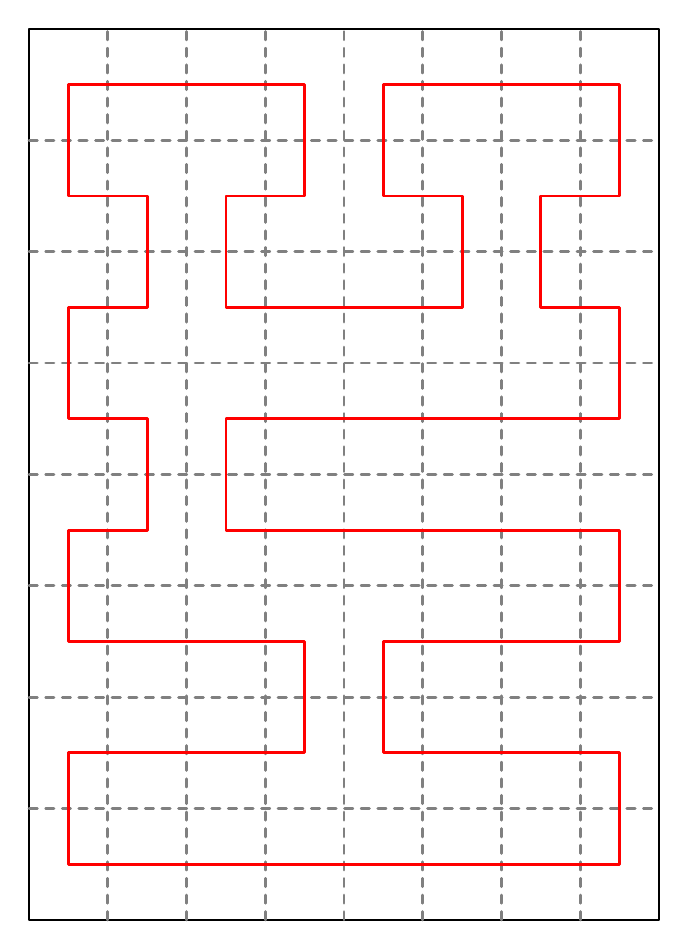
\begin{tikzpicture}[x=1.0cm,y=1.4142135623730951cm,line width=1pt,line cap=round,line join=round]
\draw (0,0) rectangle (8,8);
\draw[dashed,gray] (1,0) -- (1,8) (2,0) -- (2,8) (3,0) -- (3,8) (4,0) -- (4,8) (5,0) -- (5,8) (6,0) -- (6,8) (7,0) -- (7,8) (0,1) -- (8,1) (0,2) -- (8,2) (0,3) -- (8,3) (0,4) -- (8,4) (0,5) -- (8,5) (0,6) -- (8,6) (0,7) -- (8,7);
\draw[red] (0.5,0.5) -- (1.5,0.5) -- (2.5,0.5) -- (3.5,0.5) -- (4.5,0.5) -- (5.5,0.5) -- (6.5,0.5) -- (7.5,0.5) -- (7.5,1.5) -- (6.5,1.5) -- (5.5,1.5) -- (4.5,1.5) -- (4.5,2.5) -- (5.5,2.5) -- (6.5,2.5) -- (7.5,2.5) -- (7.5,3.5) -- (6.5,3.5) -- (5.5,3.5) -- (4.5,3.5) -- (3.5,3.5) -- (2.5,3.5) -- (2.5,4.5) -- (3.5,4.5) -- (4.5,4.5) -- (5.5,4.5) -- (6.5,4.5) -- (7.5,4.5) -- (7.5,5.5) -- (6.5,5.5) -- (6.5,6.5) -- (7.5,6.5) -- (7.5,7.5) -- (6.5,7.5) -- (5.5,7.5) -- (4.5,7.5) -- (4.5,6.5) -- (5.5,6.5) -- (5.5,5.5) -- (4.5,5.5) -- (3.5,5.5) -- (2.5,5.5) -- (2.5,6.5) -- (3.5,6.5) -- (3.5,7.5) -- (2.5,7.5) -- (1.5,7.5) -- (0.5,7.5) -- (0.5,6.5) -- (1.5,6.5) -- (1.5,5.5) -- (0.5,5.5) -- (0.5,4.5) -- (1.5,4.5) -- (1.5,3.5) -- (0.5,3.5) -- (0.5,2.5) -- (1.5,2.5) -- (2.5,2.5) -- (3.5,2.5) -- (3.5,1.5) -- (2.5,1.5) -- (1.5,1.5) -- (0.5,1.5) -- (0.5,0.5) -- cycle;\end{tikzpicture}

\vspace{5mm}

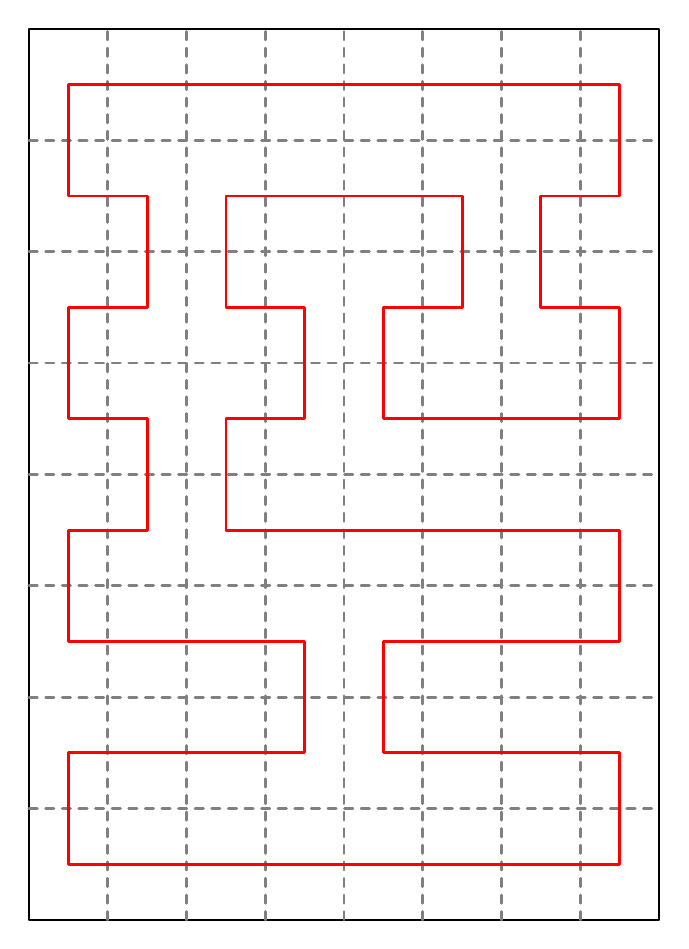
\begin{tikzpicture}[x=1.0cm,y=1.4142135623730951cm,line width=1pt,line cap=round,line join=round]
\draw (0,0) rectangle (8,8);
\draw[dashed,gray] (1,0) -- (1,8) (2,0) -- (2,8) (3,0) -- (3,8) (4,0) -- (4,8) (5,0) -- (5,8) (6,0) -- (6,8) (7,0) -- (7,8) (0,1) -- (8,1) (0,2) -- (8,2) (0,3) -- (8,3) (0,4) -- (8,4) (0,5) -- (8,5) (0,6) -- (8,6) (0,7) -- (8,7);
\draw[red] (0.5,0.5) -- (1.5,0.5) -- (2.5,0.5) -- (3.5,0.5) -- (4.5,0.5) -- (5.5,0.5) -- (6.5,0.5) -- (7.5,0.5) -- (7.5,1.5) -- (6.5,1.5) -- (5.5,1.5) -- (4.5,1.5) -- (4.5,2.5) -- (5.5,2.5) -- (6.5,2.5) -- (7.5,2.5) -- (7.5,3.5) -- (6.5,3.5) -- (5.5,3.5) -- (4.5,3.5) -- (3.5,3.5) -- (2.5,3.5) -- (2.5,4.5) -- (3.5,4.5) -- (3.5,5.5) -- (2.5,5.5) -- (2.5,6.5) -- (3.5,6.5) -- (4.5,6.5) -- (5.5,6.5) -- (5.5,5.5) -- (4.5,5.5) -- (4.5,4.5) -- (5.5,4.5) -- (6.5,4.5) -- (7.5,4.5) -- (7.5,5.5) -- (6.5,5.5) -- (6.5,6.5) -- (7.5,6.5) -- (7.5,7.5) -- (6.5,7.5) -- (5.5,7.5) -- (4.5,7.5) -- (3.5,7.5) -- (2.5,7.5) -- (1.5,7.5) -- (0.5,7.5) -- (0.5,6.5) -- (1.5,6.5) -- (1.5,5.5) -- (0.5,5.5) -- (0.5,4.5) -- (1.5,4.5) -- (1.5,3.5) -- (0.5,3.5) -- (0.5,2.5) -- (1.5,2.5) -- (2.5,2.5) -- (3.5,2.5) -- (3.5,1.5) -- (2.5,1.5) -- (1.5,1.5) -- (0.5,1.5) -- (0.5,0.5) -- cycle;\end{tikzpicture}
\hspace{5mm}
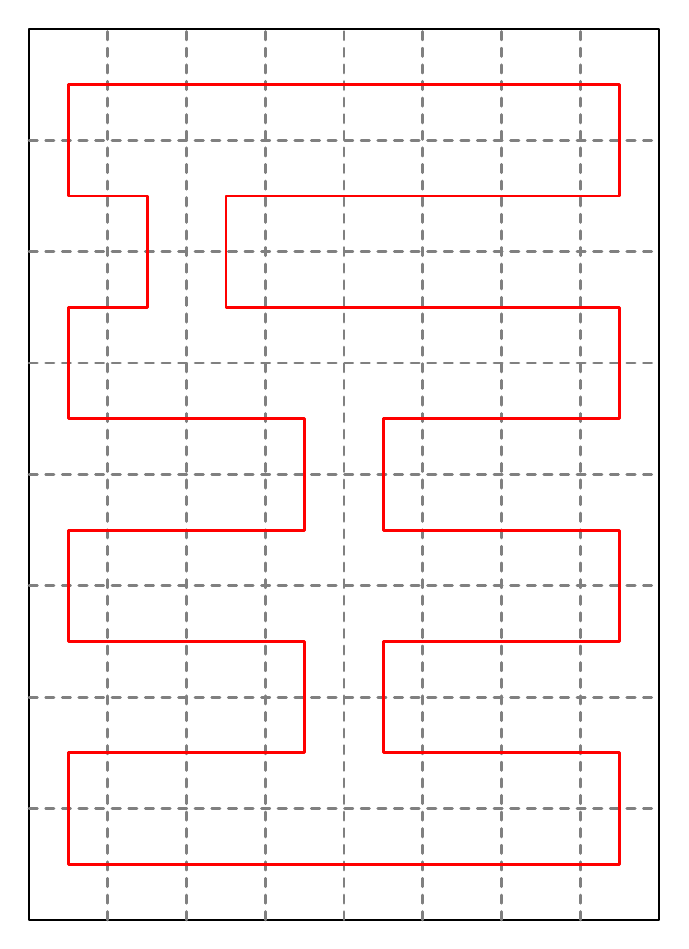
\begin{tikzpicture}[x=1.0cm,y=1.4142135623730951cm,line width=1pt,line cap=round,line join=round]
\draw (0,0) rectangle (8,8);
\draw[dashed,gray] (1,0) -- (1,8) (2,0) -- (2,8) (3,0) -- (3,8) (4,0) -- (4,8) (5,0) -- (5,8) (6,0) -- (6,8) (7,0) -- (7,8) (0,1) -- (8,1) (0,2) -- (8,2) (0,3) -- (8,3) (0,4) -- (8,4) (0,5) -- (8,5) (0,6) -- (8,6) (0,7) -- (8,7);
\draw[red] (0.5,0.5) -- (1.5,0.5) -- (2.5,0.5) -- (3.5,0.5) -- (4.5,0.5) -- (5.5,0.5) -- (6.5,0.5) -- (7.5,0.5) -- (7.5,1.5) -- (6.5,1.5) -- (5.5,1.5) -- (4.5,1.5) -- (4.5,2.5) -- (5.5,2.5) -- (6.5,2.5) -- (7.5,2.5) -- (7.5,3.5) -- (6.5,3.5) -- (5.5,3.5) -- (4.5,3.5) -- (4.5,4.5) -- (5.5,4.5) -- (6.5,4.5) -- (7.5,4.5) -- (7.5,5.5) -- (6.5,5.5) -- (5.5,5.5) -- (4.5,5.5) -- (3.5,5.5) -- (2.5,5.5) -- (2.5,6.5) -- (3.5,6.5) -- (4.5,6.5) -- (5.5,6.5) -- (6.5,6.5) -- (7.5,6.5) -- (7.5,7.5) -- (6.5,7.5) -- (5.5,7.5) -- (4.5,7.5) -- (3.5,7.5) -- (2.5,7.5) -- (1.5,7.5) -- (0.5,7.5) -- (0.5,6.5) -- (1.5,6.5) -- (1.5,5.5) -- (0.5,5.5) -- (0.5,4.5) -- (1.5,4.5) -- (2.5,4.5) -- (3.5,4.5) -- (3.5,3.5) -- (2.5,3.5) -- (1.5,3.5) -- (0.5,3.5) -- (0.5,2.5) -- (1.5,2.5) -- (2.5,2.5) -- (3.5,2.5) -- (3.5,1.5) -- (2.5,1.5) -- (1.5,1.5) -- (0.5,1.5) -- (0.5,0.5) -- cycle;\end{tikzpicture}

\vspace{5mm}

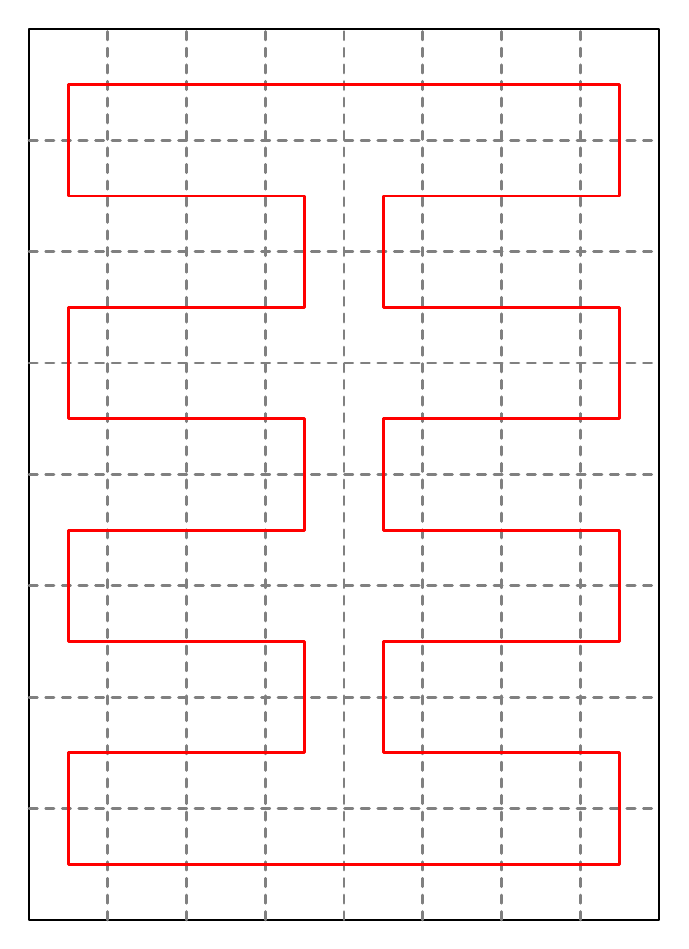
\begin{tikzpicture}[x=1.0cm,y=1.4142135623730951cm,line width=1pt,line cap=round,line join=round]
\draw (0,0) rectangle (8,8);
\draw[dashed,gray] (1,0) -- (1,8) (2,0) -- (2,8) (3,0) -- (3,8) (4,0) -- (4,8) (5,0) -- (5,8) (6,0) -- (6,8) (7,0) -- (7,8) (0,1) -- (8,1) (0,2) -- (8,2) (0,3) -- (8,3) (0,4) -- (8,4) (0,5) -- (8,5) (0,6) -- (8,6) (0,7) -- (8,7);
\draw[red] (0.5,0.5) -- (1.5,0.5) -- (2.5,0.5) -- (3.5,0.5) -- (4.5,0.5) -- (5.5,0.5) -- (6.5,0.5) -- (7.5,0.5) -- (7.5,1.5) -- (6.5,1.5) -- (5.5,1.5) -- (4.5,1.5) -- (4.5,2.5) -- (5.5,2.5) -- (6.5,2.5) -- (7.5,2.5) -- (7.5,3.5) -- (6.5,3.5) -- (5.5,3.5) -- (4.5,3.5) -- (4.5,4.5) -- (5.5,4.5) -- (6.5,4.5) -- (7.5,4.5) -- (7.5,5.5) -- (6.5,5.5) -- (5.5,5.5) -- (4.5,5.5) -- (4.5,6.5) -- (5.5,6.5) -- (6.5,6.5) -- (7.5,6.5) -- (7.5,7.5) -- (6.5,7.5) -- (5.5,7.5) -- (4.5,7.5) -- (3.5,7.5) -- (2.5,7.5) -- (1.5,7.5) -- (0.5,7.5) -- (0.5,6.5) -- (1.5,6.5) -- (2.5,6.5) -- (3.5,6.5) -- (3.5,5.5) -- (2.5,5.5) -- (1.5,5.5) -- (0.5,5.5) -- (0.5,4.5) -- (1.5,4.5) -- (2.5,4.5) -- (3.5,4.5) -- (3.5,3.5) -- (2.5,3.5) -- (1.5,3.5) -- (0.5,3.5) -- (0.5,2.5) -- (1.5,2.5) -- (2.5,2.5) -- (3.5,2.5) -- (3.5,1.5) -- (2.5,1.5) -- (1.5,1.5) -- (0.5,1.5) -- (0.5,0.5) -- cycle;\end{tikzpicture}
\hspace{5mm}
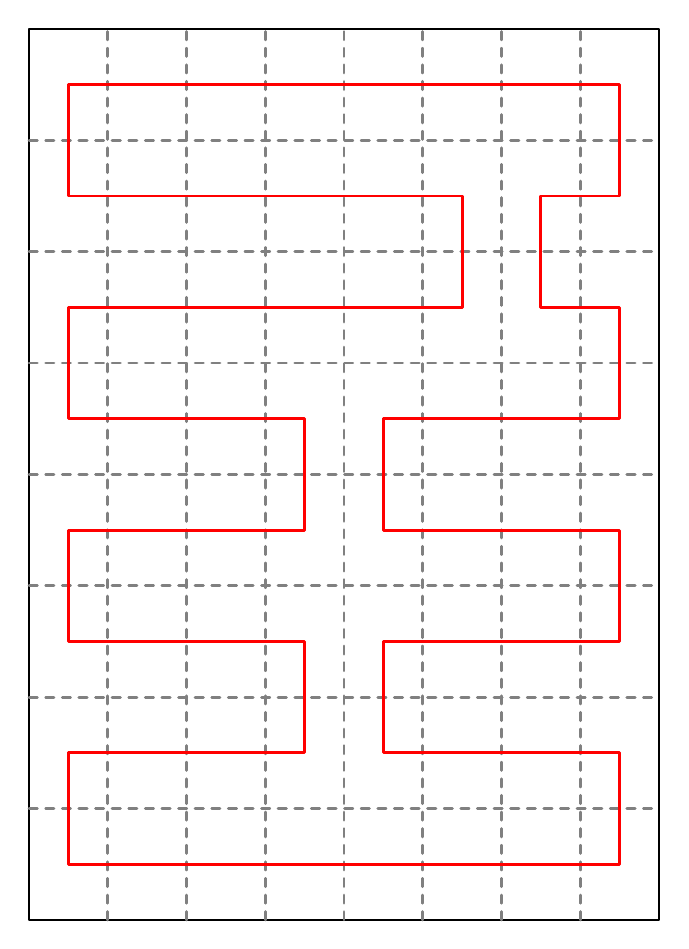
\begin{tikzpicture}[x=1.0cm,y=1.4142135623730951cm,line width=1pt,line cap=round,line join=round]
\draw (0,0) rectangle (8,8);
\draw[dashed,gray] (1,0) -- (1,8) (2,0) -- (2,8) (3,0) -- (3,8) (4,0) -- (4,8) (5,0) -- (5,8) (6,0) -- (6,8) (7,0) -- (7,8) (0,1) -- (8,1) (0,2) -- (8,2) (0,3) -- (8,3) (0,4) -- (8,4) (0,5) -- (8,5) (0,6) -- (8,6) (0,7) -- (8,7);
\draw[red] (0.5,0.5) -- (1.5,0.5) -- (2.5,0.5) -- (3.5,0.5) -- (4.5,0.5) -- (5.5,0.5) -- (6.5,0.5) -- (7.5,0.5) -- (7.5,1.5) -- (6.5,1.5) -- (5.5,1.5) -- (4.5,1.5) -- (4.5,2.5) -- (5.5,2.5) -- (6.5,2.5) -- (7.5,2.5) -- (7.5,3.5) -- (6.5,3.5) -- (5.5,3.5) -- (4.5,3.5) -- (4.5,4.5) -- (5.5,4.5) -- (6.5,4.5) -- (7.5,4.5) -- (7.5,5.5) -- (6.5,5.5) -- (6.5,6.5) -- (7.5,6.5) -- (7.5,7.5) -- (6.5,7.5) -- (5.5,7.5) -- (4.5,7.5) -- (3.5,7.5) -- (2.5,7.5) -- (1.5,7.5) -- (0.5,7.5) -- (0.5,6.5) -- (1.5,6.5) -- (2.5,6.5) -- (3.5,6.5) -- (4.5,6.5) -- (5.5,6.5) -- (5.5,5.5) -- (4.5,5.5) -- (3.5,5.5) -- (2.5,5.5) -- (1.5,5.5) -- (0.5,5.5) -- (0.5,4.5) -- (1.5,4.5) -- (2.5,4.5) -- (3.5,4.5) -- (3.5,3.5) -- (2.5,3.5) -- (1.5,3.5) -- (0.5,3.5) -- (0.5,2.5) -- (1.5,2.5) -- (2.5,2.5) -- (3.5,2.5) -- (3.5,1.5) -- (2.5,1.5) -- (1.5,1.5) -- (0.5,1.5) -- (0.5,0.5) -- cycle;\end{tikzpicture}

\vspace{5mm}

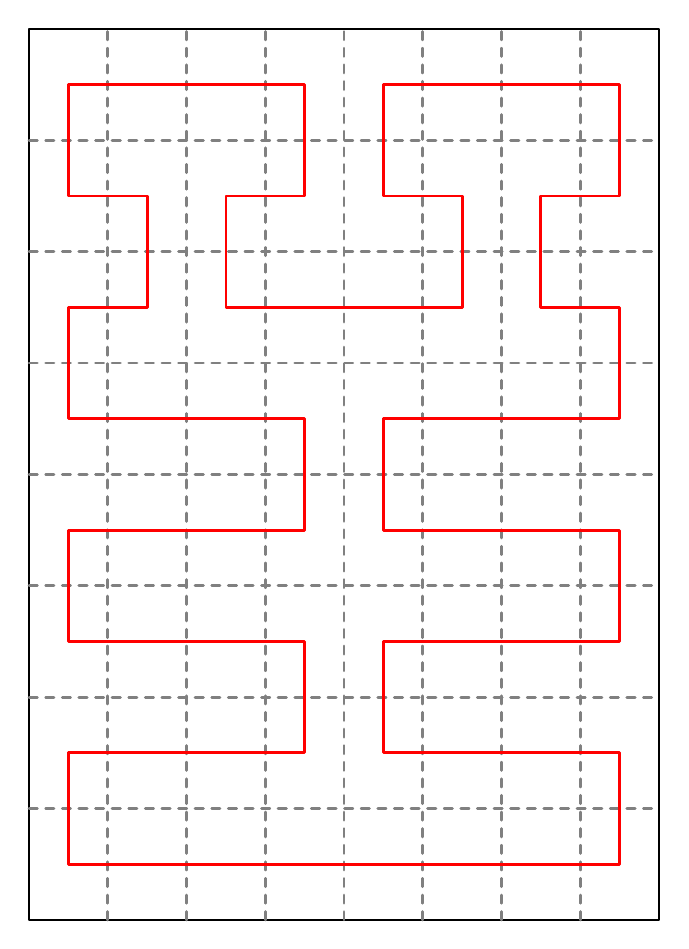
\begin{tikzpicture}[x=1.0cm,y=1.4142135623730951cm,line width=1pt,line cap=round,line join=round]
\draw (0,0) rectangle (8,8);
\draw[dashed,gray] (1,0) -- (1,8) (2,0) -- (2,8) (3,0) -- (3,8) (4,0) -- (4,8) (5,0) -- (5,8) (6,0) -- (6,8) (7,0) -- (7,8) (0,1) -- (8,1) (0,2) -- (8,2) (0,3) -- (8,3) (0,4) -- (8,4) (0,5) -- (8,5) (0,6) -- (8,6) (0,7) -- (8,7);
\draw[red] (0.5,0.5) -- (1.5,0.5) -- (2.5,0.5) -- (3.5,0.5) -- (4.5,0.5) -- (5.5,0.5) -- (6.5,0.5) -- (7.5,0.5) -- (7.5,1.5) -- (6.5,1.5) -- (5.5,1.5) -- (4.5,1.5) -- (4.5,2.5) -- (5.5,2.5) -- (6.5,2.5) -- (7.5,2.5) -- (7.5,3.5) -- (6.5,3.5) -- (5.5,3.5) -- (4.5,3.5) -- (4.5,4.5) -- (5.5,4.5) -- (6.5,4.5) -- (7.5,4.5) -- (7.5,5.5) -- (6.5,5.5) -- (6.5,6.5) -- (7.5,6.5) -- (7.5,7.5) -- (6.5,7.5) -- (5.5,7.5) -- (4.5,7.5) -- (4.5,6.5) -- (5.5,6.5) -- (5.5,5.5) -- (4.5,5.5) -- (3.5,5.5) -- (2.5,5.5) -- (2.5,6.5) -- (3.5,6.5) -- (3.5,7.5) -- (2.5,7.5) -- (1.5,7.5) -- (0.5,7.5) -- (0.5,6.5) -- (1.5,6.5) -- (1.5,5.5) -- (0.5,5.5) -- (0.5,4.5) -- (1.5,4.5) -- (2.5,4.5) -- (3.5,4.5) -- (3.5,3.5) -- (2.5,3.5) -- (1.5,3.5) -- (0.5,3.5) -- (0.5,2.5) -- (1.5,2.5) -- (2.5,2.5) -- (3.5,2.5) -- (3.5,1.5) -- (2.5,1.5) -- (1.5,1.5) -- (0.5,1.5) -- (0.5,0.5) -- cycle;\end{tikzpicture}
\hspace{5mm}
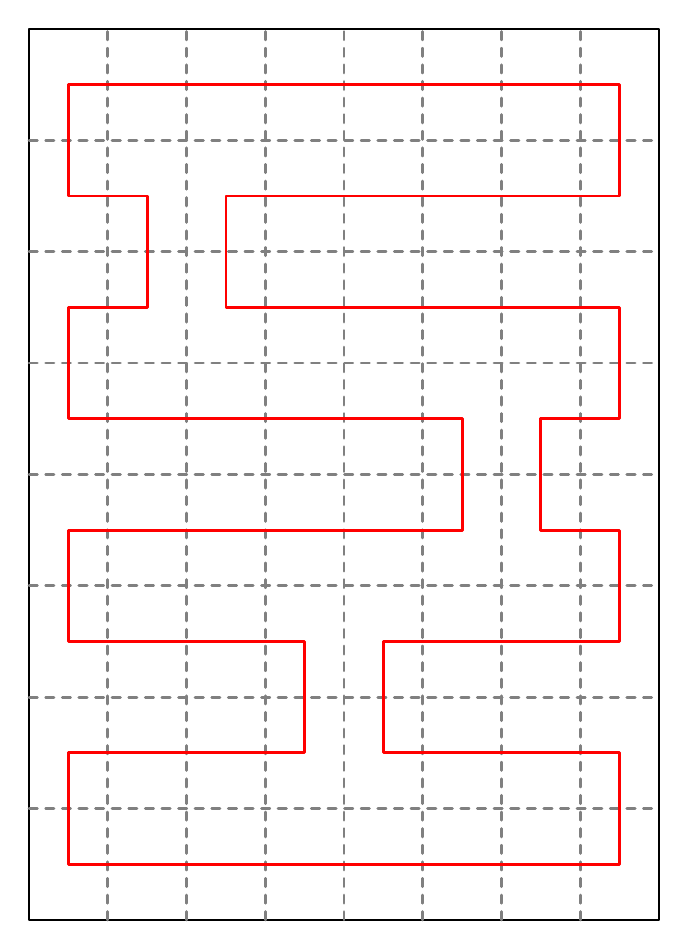
\begin{tikzpicture}[x=1.0cm,y=1.4142135623730951cm,line width=1pt,line cap=round,line join=round]
\draw (0,0) rectangle (8,8);
\draw[dashed,gray] (1,0) -- (1,8) (2,0) -- (2,8) (3,0) -- (3,8) (4,0) -- (4,8) (5,0) -- (5,8) (6,0) -- (6,8) (7,0) -- (7,8) (0,1) -- (8,1) (0,2) -- (8,2) (0,3) -- (8,3) (0,4) -- (8,4) (0,5) -- (8,5) (0,6) -- (8,6) (0,7) -- (8,7);
\draw[red] (0.5,0.5) -- (1.5,0.5) -- (2.5,0.5) -- (3.5,0.5) -- (4.5,0.5) -- (5.5,0.5) -- (6.5,0.5) -- (7.5,0.5) -- (7.5,1.5) -- (6.5,1.5) -- (5.5,1.5) -- (4.5,1.5) -- (4.5,2.5) -- (5.5,2.5) -- (6.5,2.5) -- (7.5,2.5) -- (7.5,3.5) -- (6.5,3.5) -- (6.5,4.5) -- (7.5,4.5) -- (7.5,5.5) -- (6.5,5.5) -- (5.5,5.5) -- (4.5,5.5) -- (3.5,5.5) -- (2.5,5.5) -- (2.5,6.5) -- (3.5,6.5) -- (4.5,6.5) -- (5.5,6.5) -- (6.5,6.5) -- (7.5,6.5) -- (7.5,7.5) -- (6.5,7.5) -- (5.5,7.5) -- (4.5,7.5) -- (3.5,7.5) -- (2.5,7.5) -- (1.5,7.5) -- (0.5,7.5) -- (0.5,6.5) -- (1.5,6.5) -- (1.5,5.5) -- (0.5,5.5) -- (0.5,4.5) -- (1.5,4.5) -- (2.5,4.5) -- (3.5,4.5) -- (4.5,4.5) -- (5.5,4.5) -- (5.5,3.5) -- (4.5,3.5) -- (3.5,3.5) -- (2.5,3.5) -- (1.5,3.5) -- (0.5,3.5) -- (0.5,2.5) -- (1.5,2.5) -- (2.5,2.5) -- (3.5,2.5) -- (3.5,1.5) -- (2.5,1.5) -- (1.5,1.5) -- (0.5,1.5) -- (0.5,0.5) -- cycle;\end{tikzpicture}

\vspace{5mm}

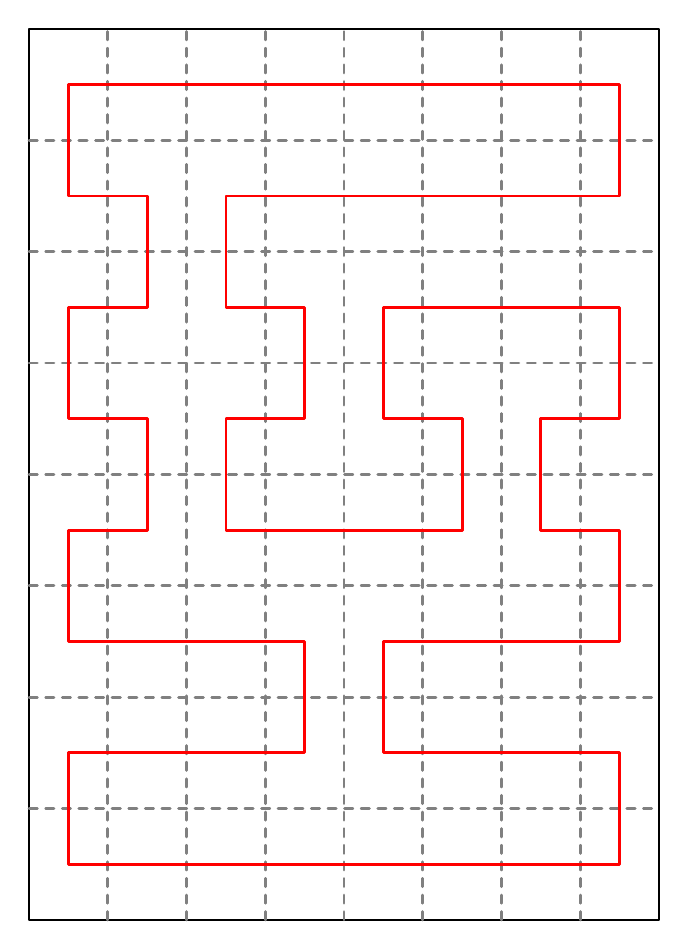
\begin{tikzpicture}[x=1.0cm,y=1.4142135623730951cm,line width=1pt,line cap=round,line join=round]
\draw (0,0) rectangle (8,8);
\draw[dashed,gray] (1,0) -- (1,8) (2,0) -- (2,8) (3,0) -- (3,8) (4,0) -- (4,8) (5,0) -- (5,8) (6,0) -- (6,8) (7,0) -- (7,8) (0,1) -- (8,1) (0,2) -- (8,2) (0,3) -- (8,3) (0,4) -- (8,4) (0,5) -- (8,5) (0,6) -- (8,6) (0,7) -- (8,7);
\draw[red] (0.5,0.5) -- (1.5,0.5) -- (2.5,0.5) -- (3.5,0.5) -- (4.5,0.5) -- (5.5,0.5) -- (6.5,0.5) -- (7.5,0.5) -- (7.5,1.5) -- (6.5,1.5) -- (5.5,1.5) -- (4.5,1.5) -- (4.5,2.5) -- (5.5,2.5) -- (6.5,2.5) -- (7.5,2.5) -- (7.5,3.5) -- (6.5,3.5) -- (6.5,4.5) -- (7.5,4.5) -- (7.5,5.5) -- (6.5,5.5) -- (5.5,5.5) -- (4.5,5.5) -- (4.5,4.5) -- (5.5,4.5) -- (5.5,3.5) -- (4.5,3.5) -- (3.5,3.5) -- (2.5,3.5) -- (2.5,4.5) -- (3.5,4.5) -- (3.5,5.5) -- (2.5,5.5) -- (2.5,6.5) -- (3.5,6.5) -- (4.5,6.5) -- (5.5,6.5) -- (6.5,6.5) -- (7.5,6.5) -- (7.5,7.5) -- (6.5,7.5) -- (5.5,7.5) -- (4.5,7.5) -- (3.5,7.5) -- (2.5,7.5) -- (1.5,7.5) -- (0.5,7.5) -- (0.5,6.5) -- (1.5,6.5) -- (1.5,5.5) -- (0.5,5.5) -- (0.5,4.5) -- (1.5,4.5) -- (1.5,3.5) -- (0.5,3.5) -- (0.5,2.5) -- (1.5,2.5) -- (2.5,2.5) -- (3.5,2.5) -- (3.5,1.5) -- (2.5,1.5) -- (1.5,1.5) -- (0.5,1.5) -- (0.5,0.5) -- cycle;\end{tikzpicture}
\hspace{5mm}
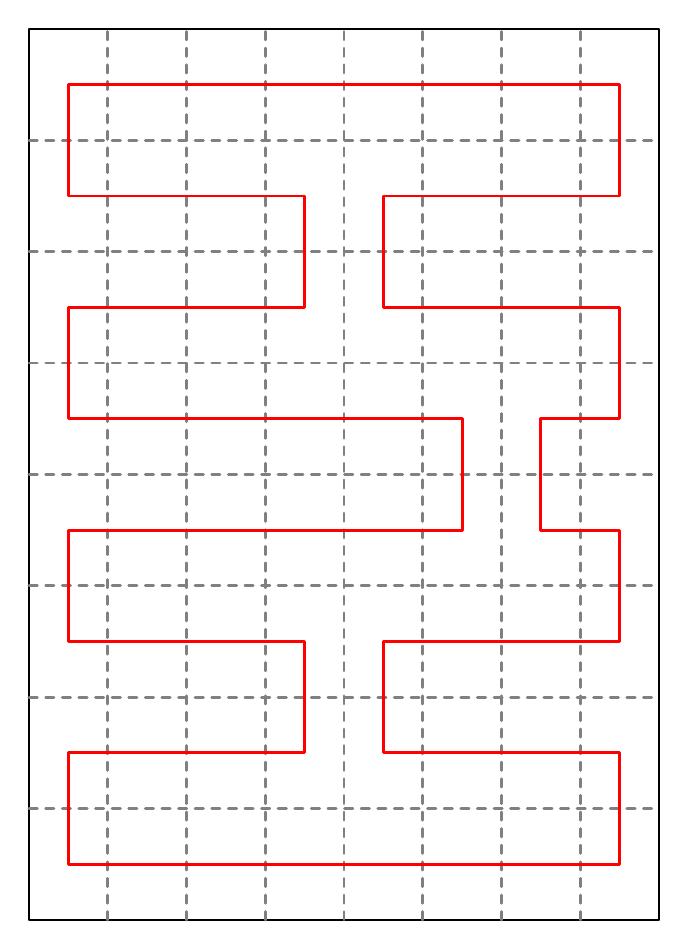
\begin{tikzpicture}[x=1.0cm,y=1.4142135623730951cm,line width=1pt,line cap=round,line join=round]
\draw (0,0) rectangle (8,8);
\draw[dashed,gray] (1,0) -- (1,8) (2,0) -- (2,8) (3,0) -- (3,8) (4,0) -- (4,8) (5,0) -- (5,8) (6,0) -- (6,8) (7,0) -- (7,8) (0,1) -- (8,1) (0,2) -- (8,2) (0,3) -- (8,3) (0,4) -- (8,4) (0,5) -- (8,5) (0,6) -- (8,6) (0,7) -- (8,7);
\draw[red] (0.5,0.5) -- (1.5,0.5) -- (2.5,0.5) -- (3.5,0.5) -- (4.5,0.5) -- (5.5,0.5) -- (6.5,0.5) -- (7.5,0.5) -- (7.5,1.5) -- (6.5,1.5) -- (5.5,1.5) -- (4.5,1.5) -- (4.5,2.5) -- (5.5,2.5) -- (6.5,2.5) -- (7.5,2.5) -- (7.5,3.5) -- (6.5,3.5) -- (6.5,4.5) -- (7.5,4.5) -- (7.5,5.5) -- (6.5,5.5) -- (5.5,5.5) -- (4.5,5.5) -- (4.5,6.5) -- (5.5,6.5) -- (6.5,6.5) -- (7.5,6.5) -- (7.5,7.5) -- (6.5,7.5) -- (5.5,7.5) -- (4.5,7.5) -- (3.5,7.5) -- (2.5,7.5) -- (1.5,7.5) -- (0.5,7.5) -- (0.5,6.5) -- (1.5,6.5) -- (2.5,6.5) -- (3.5,6.5) -- (3.5,5.5) -- (2.5,5.5) -- (1.5,5.5) -- (0.5,5.5) -- (0.5,4.5) -- (1.5,4.5) -- (2.5,4.5) -- (3.5,4.5) -- (4.5,4.5) -- (5.5,4.5) -- (5.5,3.5) -- (4.5,3.5) -- (3.5,3.5) -- (2.5,3.5) -- (1.5,3.5) -- (0.5,3.5) -- (0.5,2.5) -- (1.5,2.5) -- (2.5,2.5) -- (3.5,2.5) -- (3.5,1.5) -- (2.5,1.5) -- (1.5,1.5) -- (0.5,1.5) -- (0.5,0.5) -- cycle;\end{tikzpicture}

\vspace{5mm}

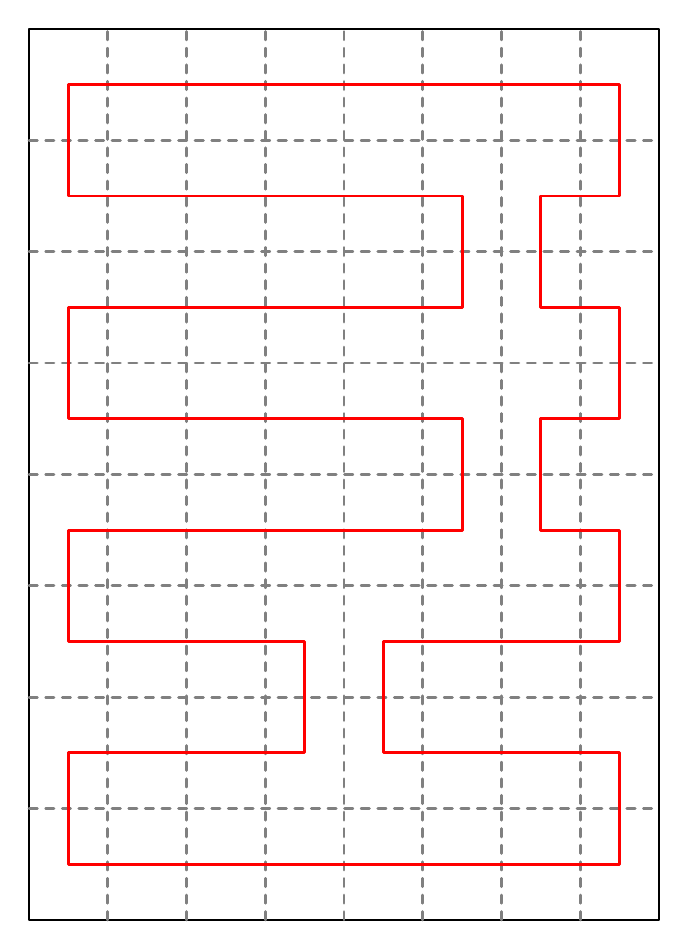
\begin{tikzpicture}[x=1.0cm,y=1.4142135623730951cm,line width=1pt,line cap=round,line join=round]
\draw (0,0) rectangle (8,8);
\draw[dashed,gray] (1,0) -- (1,8) (2,0) -- (2,8) (3,0) -- (3,8) (4,0) -- (4,8) (5,0) -- (5,8) (6,0) -- (6,8) (7,0) -- (7,8) (0,1) -- (8,1) (0,2) -- (8,2) (0,3) -- (8,3) (0,4) -- (8,4) (0,5) -- (8,5) (0,6) -- (8,6) (0,7) -- (8,7);
\draw[red] (0.5,0.5) -- (1.5,0.5) -- (2.5,0.5) -- (3.5,0.5) -- (4.5,0.5) -- (5.5,0.5) -- (6.5,0.5) -- (7.5,0.5) -- (7.5,1.5) -- (6.5,1.5) -- (5.5,1.5) -- (4.5,1.5) -- (4.5,2.5) -- (5.5,2.5) -- (6.5,2.5) -- (7.5,2.5) -- (7.5,3.5) -- (6.5,3.5) -- (6.5,4.5) -- (7.5,4.5) -- (7.5,5.5) -- (6.5,5.5) -- (6.5,6.5) -- (7.5,6.5) -- (7.5,7.5) -- (6.5,7.5) -- (5.5,7.5) -- (4.5,7.5) -- (3.5,7.5) -- (2.5,7.5) -- (1.5,7.5) -- (0.5,7.5) -- (0.5,6.5) -- (1.5,6.5) -- (2.5,6.5) -- (3.5,6.5) -- (4.5,6.5) -- (5.5,6.5) -- (5.5,5.5) -- (4.5,5.5) -- (3.5,5.5) -- (2.5,5.5) -- (1.5,5.5) -- (0.5,5.5) -- (0.5,4.5) -- (1.5,4.5) -- (2.5,4.5) -- (3.5,4.5) -- (4.5,4.5) -- (5.5,4.5) -- (5.5,3.5) -- (4.5,3.5) -- (3.5,3.5) -- (2.5,3.5) -- (1.5,3.5) -- (0.5,3.5) -- (0.5,2.5) -- (1.5,2.5) -- (2.5,2.5) -- (3.5,2.5) -- (3.5,1.5) -- (2.5,1.5) -- (1.5,1.5) -- (0.5,1.5) -- (0.5,0.5) -- cycle;\end{tikzpicture}
\hspace{5mm}
\begin{tikzpicture}[x=1.0cm,y=1.4142135623730951cm,line width=1pt,line cap=round,line join=round]
\draw (0,0) rectangle (8,8);
\draw[dashed,gray] (1,0) -- (1,8) (2,0) -- (2,8) (3,0) -- (3,8) (4,0) -- (4,8) (5,0) -- (5,8) (6,0) -- (6,8) (7,0) -- (7,8) (0,1) -- (8,1) (0,2) -- (8,2) (0,3) -- (8,3) (0,4) -- (8,4) (0,5) -- (8,5) (0,6) -- (8,6) (0,7) -- (8,7);
\draw[red] (0.5,0.5) -- (1.5,0.5) -- (2.5,0.5) -- (3.5,0.5) -- (4.5,0.5) -- (5.5,0.5) -- (6.5,0.5) -- (7.5,0.5) -- (7.5,1.5) -- (6.5,1.5) -- (5.5,1.5) -- (4.5,1.5) -- (4.5,2.5) -- (5.5,2.5) -- (6.5,2.5) -- (7.5,2.5) -- (7.5,3.5) -- (6.5,3.5) -- (6.5,4.5) -- (7.5,4.5) -- (7.5,5.5) -- (6.5,5.5) -- (6.5,6.5) -- (7.5,6.5) -- (7.5,7.5) -- (6.5,7.5) -- (5.5,7.5) -- (4.5,7.5) -- (3.5,7.5) -- (2.5,7.5) -- (1.5,7.5) -- (0.5,7.5) -- (0.5,6.5) -- (1.5,6.5) -- (2.5,6.5) -- (3.5,6.5) -- (4.5,6.5) -- (5.5,6.5) -- (5.5,5.5) -- (4.5,5.5) -- (4.5,4.5) -- (5.5,4.5) -- (5.5,3.5) -- (4.5,3.5) -- (3.5,3.5) -- (2.5,3.5) -- (2.5,4.5) -- (3.5,4.5) -- (3.5,5.5) -- (2.5,5.5) -- (1.5,5.5) -- (0.5,5.5) -- (0.5,4.5) -- (1.5,4.5) -- (1.5,3.5) -- (0.5,3.5) -- (0.5,2.5) -- (1.5,2.5) -- (2.5,2.5) -- (3.5,2.5) -- (3.5,1.5) -- (2.5,1.5) -- (1.5,1.5) -- (0.5,1.5) -- (0.5,0.5) -- cycle;\end{tikzpicture}

\vspace{5mm}

\begin{tikzpicture}[x=1.0cm,y=1.4142135623730951cm,line width=1pt,line cap=round,line join=round]
\draw (0,0) rectangle (8,8);
\draw[dashed,gray] (1,0) -- (1,8) (2,0) -- (2,8) (3,0) -- (3,8) (4,0) -- (4,8) (5,0) -- (5,8) (6,0) -- (6,8) (7,0) -- (7,8) (0,1) -- (8,1) (0,2) -- (8,2) (0,3) -- (8,3) (0,4) -- (8,4) (0,5) -- (8,5) (0,6) -- (8,6) (0,7) -- (8,7);
\draw[red] (0.5,0.5) -- (1.5,0.5) -- (2.5,0.5) -- (3.5,0.5) -- (4.5,0.5) -- (5.5,0.5) -- (6.5,0.5) -- (7.5,0.5) -- (7.5,1.5) -- (6.5,1.5) -- (5.5,1.5) -- (4.5,1.5) -- (4.5,2.5) -- (5.5,2.5) -- (6.5,2.5) -- (7.5,2.5) -- (7.5,3.5) -- (6.5,3.5) -- (6.5,4.5) -- (7.5,4.5) -- (7.5,5.5) -- (6.5,5.5) -- (6.5,6.5) -- (7.5,6.5) -- (7.5,7.5) -- (6.5,7.5) -- (5.5,7.5) -- (4.5,7.5) -- (3.5,7.5) -- (2.5,7.5) -- (1.5,7.5) -- (0.5,7.5) -- (0.5,6.5) -- (1.5,6.5) -- (1.5,5.5) -- (0.5,5.5) -- (0.5,4.5) -- (1.5,4.5) -- (2.5,4.5) -- (3.5,4.5) -- (3.5,5.5) -- (2.5,5.5) -- (2.5,6.5) -- (3.5,6.5) -- (4.5,6.5) -- (5.5,6.5) -- (5.5,5.5) -- (4.5,5.5) -- (4.5,4.5) -- (5.5,4.5) -- (5.5,3.5) -- (4.5,3.5) -- (3.5,3.5) -- (2.5,3.5) -- (1.5,3.5) -- (0.5,3.5) -- (0.5,2.5) -- (1.5,2.5) -- (2.5,2.5) -- (3.5,2.5) -- (3.5,1.5) -- (2.5,1.5) -- (1.5,1.5) -- (0.5,1.5) -- (0.5,0.5) -- cycle;\end{tikzpicture}
\hspace{5mm}
\begin{tikzpicture}[x=1.0cm,y=1.4142135623730951cm,line width=1pt,line cap=round,line join=round]
\draw (0,0) rectangle (8,8);
\draw[dashed,gray] (1,0) -- (1,8) (2,0) -- (2,8) (3,0) -- (3,8) (4,0) -- (4,8) (5,0) -- (5,8) (6,0) -- (6,8) (7,0) -- (7,8) (0,1) -- (8,1) (0,2) -- (8,2) (0,3) -- (8,3) (0,4) -- (8,4) (0,5) -- (8,5) (0,6) -- (8,6) (0,7) -- (8,7);
\draw[red] (0.5,0.5) -- (1.5,0.5) -- (2.5,0.5) -- (3.5,0.5) -- (4.5,0.5) -- (5.5,0.5) -- (6.5,0.5) -- (7.5,0.5) -- (7.5,1.5) -- (6.5,1.5) -- (5.5,1.5) -- (4.5,1.5) -- (4.5,2.5) -- (5.5,2.5) -- (6.5,2.5) -- (7.5,2.5) -- (7.5,3.5) -- (6.5,3.5) -- (6.5,4.5) -- (7.5,4.5) -- (7.5,5.5) -- (6.5,5.5) -- (6.5,6.5) -- (7.5,6.5) -- (7.5,7.5) -- (6.5,7.5) -- (5.5,7.5) -- (4.5,7.5) -- (4.5,6.5) -- (5.5,6.5) -- (5.5,5.5) -- (4.5,5.5) -- (3.5,5.5) -- (2.5,5.5) -- (2.5,6.5) -- (3.5,6.5) -- (3.5,7.5) -- (2.5,7.5) -- (1.5,7.5) -- (0.5,7.5) -- (0.5,6.5) -- (1.5,6.5) -- (1.5,5.5) -- (0.5,5.5) -- (0.5,4.5) -- (1.5,4.5) -- (2.5,4.5) -- (3.5,4.5) -- (4.5,4.5) -- (5.5,4.5) -- (5.5,3.5) -- (4.5,3.5) -- (3.5,3.5) -- (2.5,3.5) -- (1.5,3.5) -- (0.5,3.5) -- (0.5,2.5) -- (1.5,2.5) -- (2.5,2.5) -- (3.5,2.5) -- (3.5,1.5) -- (2.5,1.5) -- (1.5,1.5) -- (0.5,1.5) -- (0.5,0.5) -- cycle;\end{tikzpicture}

\vspace{5mm}

\begin{tikzpicture}[x=1.0cm,y=1.4142135623730951cm,line width=1pt,line cap=round,line join=round]
\draw (0,0) rectangle (8,8);
\draw[dashed,gray] (1,0) -- (1,8) (2,0) -- (2,8) (3,0) -- (3,8) (4,0) -- (4,8) (5,0) -- (5,8) (6,0) -- (6,8) (7,0) -- (7,8) (0,1) -- (8,1) (0,2) -- (8,2) (0,3) -- (8,3) (0,4) -- (8,4) (0,5) -- (8,5) (0,6) -- (8,6) (0,7) -- (8,7);
\draw[red] (0.5,0.5) -- (1.5,0.5) -- (2.5,0.5) -- (3.5,0.5) -- (4.5,0.5) -- (5.5,0.5) -- (6.5,0.5) -- (7.5,0.5) -- (7.5,1.5) -- (6.5,1.5) -- (5.5,1.5) -- (4.5,1.5) -- (4.5,2.5) -- (5.5,2.5) -- (6.5,2.5) -- (7.5,2.5) -- (7.5,3.5) -- (6.5,3.5) -- (6.5,4.5) -- (7.5,4.5) -- (7.5,5.5) -- (6.5,5.5) -- (6.5,6.5) -- (7.5,6.5) -- (7.5,7.5) -- (6.5,7.5) -- (5.5,7.5) -- (4.5,7.5) -- (4.5,6.5) -- (5.5,6.5) -- (5.5,5.5) -- (4.5,5.5) -- (4.5,4.5) -- (5.5,4.5) -- (5.5,3.5) -- (4.5,3.5) -- (3.5,3.5) -- (2.5,3.5) -- (2.5,4.5) -- (3.5,4.5) -- (3.5,5.5) -- (2.5,5.5) -- (2.5,6.5) -- (3.5,6.5) -- (3.5,7.5) -- (2.5,7.5) -- (1.5,7.5) -- (0.5,7.5) -- (0.5,6.5) -- (1.5,6.5) -- (1.5,5.5) -- (0.5,5.5) -- (0.5,4.5) -- (1.5,4.5) -- (1.5,3.5) -- (0.5,3.5) -- (0.5,2.5) -- (1.5,2.5) -- (2.5,2.5) -- (3.5,2.5) -- (3.5,1.5) -- (2.5,1.5) -- (1.5,1.5) -- (0.5,1.5) -- (0.5,0.5) -- cycle;\end{tikzpicture}
\hspace{5mm}
\begin{tikzpicture}[x=1.0cm,y=1.4142135623730951cm,line width=1pt,line cap=round,line join=round]
\draw (0,0) rectangle (8,8);
\draw[dashed,gray] (1,0) -- (1,8) (2,0) -- (2,8) (3,0) -- (3,8) (4,0) -- (4,8) (5,0) -- (5,8) (6,0) -- (6,8) (7,0) -- (7,8) (0,1) -- (8,1) (0,2) -- (8,2) (0,3) -- (8,3) (0,4) -- (8,4) (0,5) -- (8,5) (0,6) -- (8,6) (0,7) -- (8,7);
\draw[red] (0.5,0.5) -- (1.5,0.5) -- (2.5,0.5) -- (3.5,0.5) -- (4.5,0.5) -- (5.5,0.5) -- (6.5,0.5) -- (7.5,0.5) -- (7.5,1.5) -- (6.5,1.5) -- (6.5,2.5) -- (7.5,2.5) -- (7.5,3.5) -- (6.5,3.5) -- (5.5,3.5) -- (4.5,3.5) -- (3.5,3.5) -- (2.5,3.5) -- (2.5,4.5) -- (3.5,4.5) -- (4.5,4.5) -- (5.5,4.5) -- (6.5,4.5) -- (7.5,4.5) -- (7.5,5.5) -- (6.5,5.5) -- (5.5,5.5) -- (4.5,5.5) -- (3.5,5.5) -- (2.5,5.5) -- (2.5,6.5) -- (3.5,6.5) -- (4.5,6.5) -- (5.5,6.5) -- (6.5,6.5) -- (7.5,6.5) -- (7.5,7.5) -- (6.5,7.5) -- (5.5,7.5) -- (4.5,7.5) -- (3.5,7.5) -- (2.5,7.5) -- (1.5,7.5) -- (0.5,7.5) -- (0.5,6.5) -- (1.5,6.5) -- (1.5,5.5) -- (0.5,5.5) -- (0.5,4.5) -- (1.5,4.5) -- (1.5,3.5) -- (0.5,3.5) -- (0.5,2.5) -- (1.5,2.5) -- (2.5,2.5) -- (3.5,2.5) -- (4.5,2.5) -- (5.5,2.5) -- (5.5,1.5) -- (4.5,1.5) -- (3.5,1.5) -- (2.5,1.5) -- (1.5,1.5) -- (0.5,1.5) -- (0.5,0.5) -- cycle;\end{tikzpicture}

\vspace{5mm}

\begin{tikzpicture}[x=1.0cm,y=1.4142135623730951cm,line width=1pt,line cap=round,line join=round]
\draw (0,0) rectangle (8,8);
\draw[dashed,gray] (1,0) -- (1,8) (2,0) -- (2,8) (3,0) -- (3,8) (4,0) -- (4,8) (5,0) -- (5,8) (6,0) -- (6,8) (7,0) -- (7,8) (0,1) -- (8,1) (0,2) -- (8,2) (0,3) -- (8,3) (0,4) -- (8,4) (0,5) -- (8,5) (0,6) -- (8,6) (0,7) -- (8,7);
\draw[red] (0.5,0.5) -- (1.5,0.5) -- (2.5,0.5) -- (3.5,0.5) -- (4.5,0.5) -- (5.5,0.5) -- (6.5,0.5) -- (7.5,0.5) -- (7.5,1.5) -- (6.5,1.5) -- (6.5,2.5) -- (7.5,2.5) -- (7.5,3.5) -- (6.5,3.5) -- (5.5,3.5) -- (4.5,3.5) -- (3.5,3.5) -- (2.5,3.5) -- (2.5,4.5) -- (3.5,4.5) -- (4.5,4.5) -- (5.5,4.5) -- (6.5,4.5) -- (7.5,4.5) -- (7.5,5.5) -- (6.5,5.5) -- (5.5,5.5) -- (4.5,5.5) -- (4.5,6.5) -- (5.5,6.5) -- (6.5,6.5) -- (7.5,6.5) -- (7.5,7.5) -- (6.5,7.5) -- (5.5,7.5) -- (4.5,7.5) -- (3.5,7.5) -- (2.5,7.5) -- (1.5,7.5) -- (0.5,7.5) -- (0.5,6.5) -- (1.5,6.5) -- (2.5,6.5) -- (3.5,6.5) -- (3.5,5.5) -- (2.5,5.5) -- (1.5,5.5) -- (0.5,5.5) -- (0.5,4.5) -- (1.5,4.5) -- (1.5,3.5) -- (0.5,3.5) -- (0.5,2.5) -- (1.5,2.5) -- (2.5,2.5) -- (3.5,2.5) -- (4.5,2.5) -- (5.5,2.5) -- (5.5,1.5) -- (4.5,1.5) -- (3.5,1.5) -- (2.5,1.5) -- (1.5,1.5) -- (0.5,1.5) -- (0.5,0.5) -- cycle;\end{tikzpicture}
\hspace{5mm}
\begin{tikzpicture}[x=1.0cm,y=1.4142135623730951cm,line width=1pt,line cap=round,line join=round]
\draw (0,0) rectangle (8,8);
\draw[dashed,gray] (1,0) -- (1,8) (2,0) -- (2,8) (3,0) -- (3,8) (4,0) -- (4,8) (5,0) -- (5,8) (6,0) -- (6,8) (7,0) -- (7,8) (0,1) -- (8,1) (0,2) -- (8,2) (0,3) -- (8,3) (0,4) -- (8,4) (0,5) -- (8,5) (0,6) -- (8,6) (0,7) -- (8,7);
\draw[red] (0.5,0.5) -- (1.5,0.5) -- (2.5,0.5) -- (3.5,0.5) -- (4.5,0.5) -- (5.5,0.5) -- (6.5,0.5) -- (7.5,0.5) -- (7.5,1.5) -- (6.5,1.5) -- (6.5,2.5) -- (7.5,2.5) -- (7.5,3.5) -- (6.5,3.5) -- (5.5,3.5) -- (4.5,3.5) -- (3.5,3.5) -- (2.5,3.5) -- (2.5,4.5) -- (3.5,4.5) -- (4.5,4.5) -- (5.5,4.5) -- (6.5,4.5) -- (7.5,4.5) -- (7.5,5.5) -- (6.5,5.5) -- (6.5,6.5) -- (7.5,6.5) -- (7.5,7.5) -- (6.5,7.5) -- (5.5,7.5) -- (4.5,7.5) -- (3.5,7.5) -- (2.5,7.5) -- (1.5,7.5) -- (0.5,7.5) -- (0.5,6.5) -- (1.5,6.5) -- (2.5,6.5) -- (3.5,6.5) -- (4.5,6.5) -- (5.5,6.5) -- (5.5,5.5) -- (4.5,5.5) -- (3.5,5.5) -- (2.5,5.5) -- (1.5,5.5) -- (0.5,5.5) -- (0.5,4.5) -- (1.5,4.5) -- (1.5,3.5) -- (0.5,3.5) -- (0.5,2.5) -- (1.5,2.5) -- (2.5,2.5) -- (3.5,2.5) -- (4.5,2.5) -- (5.5,2.5) -- (5.5,1.5) -- (4.5,1.5) -- (3.5,1.5) -- (2.5,1.5) -- (1.5,1.5) -- (0.5,1.5) -- (0.5,0.5) -- cycle;\end{tikzpicture}

\vspace{5mm}

\begin{tikzpicture}[x=1.0cm,y=1.4142135623730951cm,line width=1pt,line cap=round,line join=round]
\draw (0,0) rectangle (8,8);
\draw[dashed,gray] (1,0) -- (1,8) (2,0) -- (2,8) (3,0) -- (3,8) (4,0) -- (4,8) (5,0) -- (5,8) (6,0) -- (6,8) (7,0) -- (7,8) (0,1) -- (8,1) (0,2) -- (8,2) (0,3) -- (8,3) (0,4) -- (8,4) (0,5) -- (8,5) (0,6) -- (8,6) (0,7) -- (8,7);
\draw[red] (0.5,0.5) -- (1.5,0.5) -- (2.5,0.5) -- (3.5,0.5) -- (4.5,0.5) -- (5.5,0.5) -- (6.5,0.5) -- (7.5,0.5) -- (7.5,1.5) -- (6.5,1.5) -- (6.5,2.5) -- (7.5,2.5) -- (7.5,3.5) -- (6.5,3.5) -- (5.5,3.5) -- (4.5,3.5) -- (3.5,3.5) -- (2.5,3.5) -- (2.5,4.5) -- (3.5,4.5) -- (4.5,4.5) -- (5.5,4.5) -- (6.5,4.5) -- (7.5,4.5) -- (7.5,5.5) -- (6.5,5.5) -- (6.5,6.5) -- (7.5,6.5) -- (7.5,7.5) -- (6.5,7.5) -- (5.5,7.5) -- (4.5,7.5) -- (4.5,6.5) -- (5.5,6.5) -- (5.5,5.5) -- (4.5,5.5) -- (3.5,5.5) -- (2.5,5.5) -- (2.5,6.5) -- (3.5,6.5) -- (3.5,7.5) -- (2.5,7.5) -- (1.5,7.5) -- (0.5,7.5) -- (0.5,6.5) -- (1.5,6.5) -- (1.5,5.5) -- (0.5,5.5) -- (0.5,4.5) -- (1.5,4.5) -- (1.5,3.5) -- (0.5,3.5) -- (0.5,2.5) -- (1.5,2.5) -- (2.5,2.5) -- (3.5,2.5) -- (4.5,2.5) -- (5.5,2.5) -- (5.5,1.5) -- (4.5,1.5) -- (3.5,1.5) -- (2.5,1.5) -- (1.5,1.5) -- (0.5,1.5) -- (0.5,0.5) -- cycle;\end{tikzpicture}
\hspace{5mm}
\begin{tikzpicture}[x=1.0cm,y=1.4142135623730951cm,line width=1pt,line cap=round,line join=round]
\draw (0,0) rectangle (8,8);
\draw[dashed,gray] (1,0) -- (1,8) (2,0) -- (2,8) (3,0) -- (3,8) (4,0) -- (4,8) (5,0) -- (5,8) (6,0) -- (6,8) (7,0) -- (7,8) (0,1) -- (8,1) (0,2) -- (8,2) (0,3) -- (8,3) (0,4) -- (8,4) (0,5) -- (8,5) (0,6) -- (8,6) (0,7) -- (8,7);
\draw[red] (0.5,0.5) -- (1.5,0.5) -- (2.5,0.5) -- (3.5,0.5) -- (4.5,0.5) -- (5.5,0.5) -- (6.5,0.5) -- (7.5,0.5) -- (7.5,1.5) -- (6.5,1.5) -- (6.5,2.5) -- (7.5,2.5) -- (7.5,3.5) -- (6.5,3.5) -- (5.5,3.5) -- (4.5,3.5) -- (3.5,3.5) -- (2.5,3.5) -- (2.5,4.5) -- (3.5,4.5) -- (3.5,5.5) -- (2.5,5.5) -- (2.5,6.5) -- (3.5,6.5) -- (4.5,6.5) -- (5.5,6.5) -- (5.5,5.5) -- (4.5,5.5) -- (4.5,4.5) -- (5.5,4.5) -- (6.5,4.5) -- (7.5,4.5) -- (7.5,5.5) -- (6.5,5.5) -- (6.5,6.5) -- (7.5,6.5) -- (7.5,7.5) -- (6.5,7.5) -- (5.5,7.5) -- (4.5,7.5) -- (3.5,7.5) -- (2.5,7.5) -- (1.5,7.5) -- (0.5,7.5) -- (0.5,6.5) -- (1.5,6.5) -- (1.5,5.5) -- (0.5,5.5) -- (0.5,4.5) -- (1.5,4.5) -- (1.5,3.5) -- (0.5,3.5) -- (0.5,2.5) -- (1.5,2.5) -- (2.5,2.5) -- (3.5,2.5) -- (4.5,2.5) -- (5.5,2.5) -- (5.5,1.5) -- (4.5,1.5) -- (3.5,1.5) -- (2.5,1.5) -- (1.5,1.5) -- (0.5,1.5) -- (0.5,0.5) -- cycle;\end{tikzpicture}

\vspace{5mm}

\begin{tikzpicture}[x=1.0cm,y=1.4142135623730951cm,line width=1pt,line cap=round,line join=round]
\draw (0,0) rectangle (8,8);
\draw[dashed,gray] (1,0) -- (1,8) (2,0) -- (2,8) (3,0) -- (3,8) (4,0) -- (4,8) (5,0) -- (5,8) (6,0) -- (6,8) (7,0) -- (7,8) (0,1) -- (8,1) (0,2) -- (8,2) (0,3) -- (8,3) (0,4) -- (8,4) (0,5) -- (8,5) (0,6) -- (8,6) (0,7) -- (8,7);
\draw[red] (0.5,0.5) -- (1.5,0.5) -- (2.5,0.5) -- (3.5,0.5) -- (4.5,0.5) -- (5.5,0.5) -- (6.5,0.5) -- (7.5,0.5) -- (7.5,1.5) -- (6.5,1.5) -- (6.5,2.5) -- (7.5,2.5) -- (7.5,3.5) -- (6.5,3.5) -- (5.5,3.5) -- (4.5,3.5) -- (4.5,2.5) -- (5.5,2.5) -- (5.5,1.5) -- (4.5,1.5) -- (3.5,1.5) -- (2.5,1.5) -- (2.5,2.5) -- (3.5,2.5) -- (3.5,3.5) -- (2.5,3.5) -- (2.5,4.5) -- (3.5,4.5) -- (4.5,4.5) -- (5.5,4.5) -- (6.5,4.5) -- (7.5,4.5) -- (7.5,5.5) -- (6.5,5.5) -- (5.5,5.5) -- (4.5,5.5) -- (3.5,5.5) -- (2.5,5.5) -- (2.5,6.5) -- (3.5,6.5) -- (4.5,6.5) -- (5.5,6.5) -- (6.5,6.5) -- (7.5,6.5) -- (7.5,7.5) -- (6.5,7.5) -- (5.5,7.5) -- (4.5,7.5) -- (3.5,7.5) -- (2.5,7.5) -- (1.5,7.5) -- (0.5,7.5) -- (0.5,6.5) -- (1.5,6.5) -- (1.5,5.5) -- (0.5,5.5) -- (0.5,4.5) -- (1.5,4.5) -- (1.5,3.5) -- (0.5,3.5) -- (0.5,2.5) -- (1.5,2.5) -- (1.5,1.5) -- (0.5,1.5) -- (0.5,0.5) -- cycle;\end{tikzpicture}
\hspace{5mm}
\begin{tikzpicture}[x=1.0cm,y=1.4142135623730951cm,line width=1pt,line cap=round,line join=round]
\draw (0,0) rectangle (8,8);
\draw[dashed,gray] (1,0) -- (1,8) (2,0) -- (2,8) (3,0) -- (3,8) (4,0) -- (4,8) (5,0) -- (5,8) (6,0) -- (6,8) (7,0) -- (7,8) (0,1) -- (8,1) (0,2) -- (8,2) (0,3) -- (8,3) (0,4) -- (8,4) (0,5) -- (8,5) (0,6) -- (8,6) (0,7) -- (8,7);
\draw[red] (0.5,0.5) -- (1.5,0.5) -- (2.5,0.5) -- (3.5,0.5) -- (4.5,0.5) -- (5.5,0.5) -- (6.5,0.5) -- (7.5,0.5) -- (7.5,1.5) -- (6.5,1.5) -- (6.5,2.5) -- (7.5,2.5) -- (7.5,3.5) -- (6.5,3.5) -- (5.5,3.5) -- (4.5,3.5) -- (4.5,2.5) -- (5.5,2.5) -- (5.5,1.5) -- (4.5,1.5) -- (3.5,1.5) -- (2.5,1.5) -- (2.5,2.5) -- (3.5,2.5) -- (3.5,3.5) -- (2.5,3.5) -- (2.5,4.5) -- (3.5,4.5) -- (4.5,4.5) -- (5.5,4.5) -- (6.5,4.5) -- (7.5,4.5) -- (7.5,5.5) -- (6.5,5.5) -- (5.5,5.5) -- (4.5,5.5) -- (4.5,6.5) -- (5.5,6.5) -- (6.5,6.5) -- (7.5,6.5) -- (7.5,7.5) -- (6.5,7.5) -- (5.5,7.5) -- (4.5,7.5) -- (3.5,7.5) -- (2.5,7.5) -- (1.5,7.5) -- (0.5,7.5) -- (0.5,6.5) -- (1.5,6.5) -- (2.5,6.5) -- (3.5,6.5) -- (3.5,5.5) -- (2.5,5.5) -- (1.5,5.5) -- (0.5,5.5) -- (0.5,4.5) -- (1.5,4.5) -- (1.5,3.5) -- (0.5,3.5) -- (0.5,2.5) -- (1.5,2.5) -- (1.5,1.5) -- (0.5,1.5) -- (0.5,0.5) -- cycle;\end{tikzpicture}

\vspace{5mm}

\begin{tikzpicture}[x=1.0cm,y=1.4142135623730951cm,line width=1pt,line cap=round,line join=round]
\draw (0,0) rectangle (8,8);
\draw[dashed,gray] (1,0) -- (1,8) (2,0) -- (2,8) (3,0) -- (3,8) (4,0) -- (4,8) (5,0) -- (5,8) (6,0) -- (6,8) (7,0) -- (7,8) (0,1) -- (8,1) (0,2) -- (8,2) (0,3) -- (8,3) (0,4) -- (8,4) (0,5) -- (8,5) (0,6) -- (8,6) (0,7) -- (8,7);
\draw[red] (0.5,0.5) -- (1.5,0.5) -- (2.5,0.5) -- (3.5,0.5) -- (4.5,0.5) -- (5.5,0.5) -- (6.5,0.5) -- (7.5,0.5) -- (7.5,1.5) -- (6.5,1.5) -- (6.5,2.5) -- (7.5,2.5) -- (7.5,3.5) -- (6.5,3.5) -- (5.5,3.5) -- (4.5,3.5) -- (4.5,2.5) -- (5.5,2.5) -- (5.5,1.5) -- (4.5,1.5) -- (3.5,1.5) -- (2.5,1.5) -- (2.5,2.5) -- (3.5,2.5) -- (3.5,3.5) -- (2.5,3.5) -- (2.5,4.5) -- (3.5,4.5) -- (4.5,4.5) -- (5.5,4.5) -- (6.5,4.5) -- (7.5,4.5) -- (7.5,5.5) -- (6.5,5.5) -- (6.5,6.5) -- (7.5,6.5) -- (7.5,7.5) -- (6.5,7.5) -- (5.5,7.5) -- (4.5,7.5) -- (3.5,7.5) -- (2.5,7.5) -- (1.5,7.5) -- (0.5,7.5) -- (0.5,6.5) -- (1.5,6.5) -- (2.5,6.5) -- (3.5,6.5) -- (4.5,6.5) -- (5.5,6.5) -- (5.5,5.5) -- (4.5,5.5) -- (3.5,5.5) -- (2.5,5.5) -- (1.5,5.5) -- (0.5,5.5) -- (0.5,4.5) -- (1.5,4.5) -- (1.5,3.5) -- (0.5,3.5) -- (0.5,2.5) -- (1.5,2.5) -- (1.5,1.5) -- (0.5,1.5) -- (0.5,0.5) -- cycle;\end{tikzpicture}
\hspace{5mm}
\begin{tikzpicture}[x=1.0cm,y=1.4142135623730951cm,line width=1pt,line cap=round,line join=round]
\draw (0,0) rectangle (8,8);
\draw[dashed,gray] (1,0) -- (1,8) (2,0) -- (2,8) (3,0) -- (3,8) (4,0) -- (4,8) (5,0) -- (5,8) (6,0) -- (6,8) (7,0) -- (7,8) (0,1) -- (8,1) (0,2) -- (8,2) (0,3) -- (8,3) (0,4) -- (8,4) (0,5) -- (8,5) (0,6) -- (8,6) (0,7) -- (8,7);
\draw[red] (0.5,0.5) -- (1.5,0.5) -- (2.5,0.5) -- (3.5,0.5) -- (4.5,0.5) -- (5.5,0.5) -- (6.5,0.5) -- (7.5,0.5) -- (7.5,1.5) -- (6.5,1.5) -- (6.5,2.5) -- (7.5,2.5) -- (7.5,3.5) -- (6.5,3.5) -- (5.5,3.5) -- (4.5,3.5) -- (4.5,2.5) -- (5.5,2.5) -- (5.5,1.5) -- (4.5,1.5) -- (3.5,1.5) -- (2.5,1.5) -- (2.5,2.5) -- (3.5,2.5) -- (3.5,3.5) -- (2.5,3.5) -- (2.5,4.5) -- (3.5,4.5) -- (4.5,4.5) -- (5.5,4.5) -- (6.5,4.5) -- (7.5,4.5) -- (7.5,5.5) -- (6.5,5.5) -- (6.5,6.5) -- (7.5,6.5) -- (7.5,7.5) -- (6.5,7.5) -- (5.5,7.5) -- (4.5,7.5) -- (4.5,6.5) -- (5.5,6.5) -- (5.5,5.5) -- (4.5,5.5) -- (3.5,5.5) -- (2.5,5.5) -- (2.5,6.5) -- (3.5,6.5) -- (3.5,7.5) -- (2.5,7.5) -- (1.5,7.5) -- (0.5,7.5) -- (0.5,6.5) -- (1.5,6.5) -- (1.5,5.5) -- (0.5,5.5) -- (0.5,4.5) -- (1.5,4.5) -- (1.5,3.5) -- (0.5,3.5) -- (0.5,2.5) -- (1.5,2.5) -- (1.5,1.5) -- (0.5,1.5) -- (0.5,0.5) -- cycle;\end{tikzpicture}

\vspace{5mm}

\begin{tikzpicture}[x=1.0cm,y=1.4142135623730951cm,line width=1pt,line cap=round,line join=round]
\draw (0,0) rectangle (8,8);
\draw[dashed,gray] (1,0) -- (1,8) (2,0) -- (2,8) (3,0) -- (3,8) (4,0) -- (4,8) (5,0) -- (5,8) (6,0) -- (6,8) (7,0) -- (7,8) (0,1) -- (8,1) (0,2) -- (8,2) (0,3) -- (8,3) (0,4) -- (8,4) (0,5) -- (8,5) (0,6) -- (8,6) (0,7) -- (8,7);
\draw[red] (0.5,0.5) -- (1.5,0.5) -- (2.5,0.5) -- (3.5,0.5) -- (4.5,0.5) -- (5.5,0.5) -- (6.5,0.5) -- (7.5,0.5) -- (7.5,1.5) -- (6.5,1.5) -- (6.5,2.5) -- (7.5,2.5) -- (7.5,3.5) -- (6.5,3.5) -- (5.5,3.5) -- (4.5,3.5) -- (4.5,2.5) -- (5.5,2.5) -- (5.5,1.5) -- (4.5,1.5) -- (3.5,1.5) -- (2.5,1.5) -- (2.5,2.5) -- (3.5,2.5) -- (3.5,3.5) -- (2.5,3.5) -- (2.5,4.5) -- (3.5,4.5) -- (3.5,5.5) -- (2.5,5.5) -- (2.5,6.5) -- (3.5,6.5) -- (4.5,6.5) -- (5.5,6.5) -- (5.5,5.5) -- (4.5,5.5) -- (4.5,4.5) -- (5.5,4.5) -- (6.5,4.5) -- (7.5,4.5) -- (7.5,5.5) -- (6.5,5.5) -- (6.5,6.5) -- (7.5,6.5) -- (7.5,7.5) -- (6.5,7.5) -- (5.5,7.5) -- (4.5,7.5) -- (3.5,7.5) -- (2.5,7.5) -- (1.5,7.5) -- (0.5,7.5) -- (0.5,6.5) -- (1.5,6.5) -- (1.5,5.5) -- (0.5,5.5) -- (0.5,4.5) -- (1.5,4.5) -- (1.5,3.5) -- (0.5,3.5) -- (0.5,2.5) -- (1.5,2.5) -- (1.5,1.5) -- (0.5,1.5) -- (0.5,0.5) -- cycle;\end{tikzpicture}
\hspace{5mm}
\begin{tikzpicture}[x=1.0cm,y=1.4142135623730951cm,line width=1pt,line cap=round,line join=round]
\draw (0,0) rectangle (8,8);
\draw[dashed,gray] (1,0) -- (1,8) (2,0) -- (2,8) (3,0) -- (3,8) (4,0) -- (4,8) (5,0) -- (5,8) (6,0) -- (6,8) (7,0) -- (7,8) (0,1) -- (8,1) (0,2) -- (8,2) (0,3) -- (8,3) (0,4) -- (8,4) (0,5) -- (8,5) (0,6) -- (8,6) (0,7) -- (8,7);
\draw[red] (0.5,0.5) -- (1.5,0.5) -- (2.5,0.5) -- (3.5,0.5) -- (4.5,0.5) -- (5.5,0.5) -- (6.5,0.5) -- (7.5,0.5) -- (7.5,1.5) -- (6.5,1.5) -- (6.5,2.5) -- (7.5,2.5) -- (7.5,3.5) -- (6.5,3.5) -- (5.5,3.5) -- (4.5,3.5) -- (4.5,4.5) -- (5.5,4.5) -- (6.5,4.5) -- (7.5,4.5) -- (7.5,5.5) -- (6.5,5.5) -- (5.5,5.5) -- (4.5,5.5) -- (3.5,5.5) -- (2.5,5.5) -- (2.5,6.5) -- (3.5,6.5) -- (4.5,6.5) -- (5.5,6.5) -- (6.5,6.5) -- (7.5,6.5) -- (7.5,7.5) -- (6.5,7.5) -- (5.5,7.5) -- (4.5,7.5) -- (3.5,7.5) -- (2.5,7.5) -- (1.5,7.5) -- (0.5,7.5) -- (0.5,6.5) -- (1.5,6.5) -- (1.5,5.5) -- (0.5,5.5) -- (0.5,4.5) -- (1.5,4.5) -- (2.5,4.5) -- (3.5,4.5) -- (3.5,3.5) -- (2.5,3.5) -- (1.5,3.5) -- (0.5,3.5) -- (0.5,2.5) -- (1.5,2.5) -- (2.5,2.5) -- (3.5,2.5) -- (4.5,2.5) -- (5.5,2.5) -- (5.5,1.5) -- (4.5,1.5) -- (3.5,1.5) -- (2.5,1.5) -- (1.5,1.5) -- (0.5,1.5) -- (0.5,0.5) -- cycle;\end{tikzpicture}

\vspace{5mm}

\begin{tikzpicture}[x=1.0cm,y=1.4142135623730951cm,line width=1pt,line cap=round,line join=round]
\draw (0,0) rectangle (8,8);
\draw[dashed,gray] (1,0) -- (1,8) (2,0) -- (2,8) (3,0) -- (3,8) (4,0) -- (4,8) (5,0) -- (5,8) (6,0) -- (6,8) (7,0) -- (7,8) (0,1) -- (8,1) (0,2) -- (8,2) (0,3) -- (8,3) (0,4) -- (8,4) (0,5) -- (8,5) (0,6) -- (8,6) (0,7) -- (8,7);
\draw[red] (0.5,0.5) -- (1.5,0.5) -- (2.5,0.5) -- (3.5,0.5) -- (4.5,0.5) -- (5.5,0.5) -- (6.5,0.5) -- (7.5,0.5) -- (7.5,1.5) -- (6.5,1.5) -- (6.5,2.5) -- (7.5,2.5) -- (7.5,3.5) -- (6.5,3.5) -- (5.5,3.5) -- (4.5,3.5) -- (4.5,4.5) -- (5.5,4.5) -- (6.5,4.5) -- (7.5,4.5) -- (7.5,5.5) -- (6.5,5.5) -- (5.5,5.5) -- (4.5,5.5) -- (4.5,6.5) -- (5.5,6.5) -- (6.5,6.5) -- (7.5,6.5) -- (7.5,7.5) -- (6.5,7.5) -- (5.5,7.5) -- (4.5,7.5) -- (3.5,7.5) -- (2.5,7.5) -- (1.5,7.5) -- (0.5,7.5) -- (0.5,6.5) -- (1.5,6.5) -- (2.5,6.5) -- (3.5,6.5) -- (3.5,5.5) -- (2.5,5.5) -- (1.5,5.5) -- (0.5,5.5) -- (0.5,4.5) -- (1.5,4.5) -- (2.5,4.5) -- (3.5,4.5) -- (3.5,3.5) -- (2.5,3.5) -- (1.5,3.5) -- (0.5,3.5) -- (0.5,2.5) -- (1.5,2.5) -- (2.5,2.5) -- (3.5,2.5) -- (4.5,2.5) -- (5.5,2.5) -- (5.5,1.5) -- (4.5,1.5) -- (3.5,1.5) -- (2.5,1.5) -- (1.5,1.5) -- (0.5,1.5) -- (0.5,0.5) -- cycle;\end{tikzpicture}
\hspace{5mm}
\begin{tikzpicture}[x=1.0cm,y=1.4142135623730951cm,line width=1pt,line cap=round,line join=round]
\draw (0,0) rectangle (8,8);
\draw[dashed,gray] (1,0) -- (1,8) (2,0) -- (2,8) (3,0) -- (3,8) (4,0) -- (4,8) (5,0) -- (5,8) (6,0) -- (6,8) (7,0) -- (7,8) (0,1) -- (8,1) (0,2) -- (8,2) (0,3) -- (8,3) (0,4) -- (8,4) (0,5) -- (8,5) (0,6) -- (8,6) (0,7) -- (8,7);
\draw[red] (0.5,0.5) -- (1.5,0.5) -- (2.5,0.5) -- (3.5,0.5) -- (4.5,0.5) -- (5.5,0.5) -- (6.5,0.5) -- (7.5,0.5) -- (7.5,1.5) -- (6.5,1.5) -- (6.5,2.5) -- (7.5,2.5) -- (7.5,3.5) -- (6.5,3.5) -- (5.5,3.5) -- (4.5,3.5) -- (4.5,4.5) -- (5.5,4.5) -- (6.5,4.5) -- (7.5,4.5) -- (7.5,5.5) -- (6.5,5.5) -- (6.5,6.5) -- (7.5,6.5) -- (7.5,7.5) -- (6.5,7.5) -- (5.5,7.5) -- (4.5,7.5) -- (3.5,7.5) -- (2.5,7.5) -- (1.5,7.5) -- (0.5,7.5) -- (0.5,6.5) -- (1.5,6.5) -- (2.5,6.5) -- (3.5,6.5) -- (4.5,6.5) -- (5.5,6.5) -- (5.5,5.5) -- (4.5,5.5) -- (3.5,5.5) -- (2.5,5.5) -- (1.5,5.5) -- (0.5,5.5) -- (0.5,4.5) -- (1.5,4.5) -- (2.5,4.5) -- (3.5,4.5) -- (3.5,3.5) -- (2.5,3.5) -- (1.5,3.5) -- (0.5,3.5) -- (0.5,2.5) -- (1.5,2.5) -- (2.5,2.5) -- (3.5,2.5) -- (4.5,2.5) -- (5.5,2.5) -- (5.5,1.5) -- (4.5,1.5) -- (3.5,1.5) -- (2.5,1.5) -- (1.5,1.5) -- (0.5,1.5) -- (0.5,0.5) -- cycle;\end{tikzpicture}

\vspace{5mm}

\begin{tikzpicture}[x=1.0cm,y=1.4142135623730951cm,line width=1pt,line cap=round,line join=round]
\draw (0,0) rectangle (8,8);
\draw[dashed,gray] (1,0) -- (1,8) (2,0) -- (2,8) (3,0) -- (3,8) (4,0) -- (4,8) (5,0) -- (5,8) (6,0) -- (6,8) (7,0) -- (7,8) (0,1) -- (8,1) (0,2) -- (8,2) (0,3) -- (8,3) (0,4) -- (8,4) (0,5) -- (8,5) (0,6) -- (8,6) (0,7) -- (8,7);
\draw[red] (0.5,0.5) -- (1.5,0.5) -- (2.5,0.5) -- (3.5,0.5) -- (4.5,0.5) -- (5.5,0.5) -- (6.5,0.5) -- (7.5,0.5) -- (7.5,1.5) -- (6.5,1.5) -- (6.5,2.5) -- (7.5,2.5) -- (7.5,3.5) -- (6.5,3.5) -- (5.5,3.5) -- (4.5,3.5) -- (4.5,4.5) -- (5.5,4.5) -- (6.5,4.5) -- (7.5,4.5) -- (7.5,5.5) -- (6.5,5.5) -- (6.5,6.5) -- (7.5,6.5) -- (7.5,7.5) -- (6.5,7.5) -- (5.5,7.5) -- (4.5,7.5) -- (4.5,6.5) -- (5.5,6.5) -- (5.5,5.5) -- (4.5,5.5) -- (3.5,5.5) -- (2.5,5.5) -- (2.5,6.5) -- (3.5,6.5) -- (3.5,7.5) -- (2.5,7.5) -- (1.5,7.5) -- (0.5,7.5) -- (0.5,6.5) -- (1.5,6.5) -- (1.5,5.5) -- (0.5,5.5) -- (0.5,4.5) -- (1.5,4.5) -- (2.5,4.5) -- (3.5,4.5) -- (3.5,3.5) -- (2.5,3.5) -- (1.5,3.5) -- (0.5,3.5) -- (0.5,2.5) -- (1.5,2.5) -- (2.5,2.5) -- (3.5,2.5) -- (4.5,2.5) -- (5.5,2.5) -- (5.5,1.5) -- (4.5,1.5) -- (3.5,1.5) -- (2.5,1.5) -- (1.5,1.5) -- (0.5,1.5) -- (0.5,0.5) -- cycle;\end{tikzpicture}
\hspace{5mm}
\begin{tikzpicture}[x=1.0cm,y=1.4142135623730951cm,line width=1pt,line cap=round,line join=round]
\draw (0,0) rectangle (8,8);
\draw[dashed,gray] (1,0) -- (1,8) (2,0) -- (2,8) (3,0) -- (3,8) (4,0) -- (4,8) (5,0) -- (5,8) (6,0) -- (6,8) (7,0) -- (7,8) (0,1) -- (8,1) (0,2) -- (8,2) (0,3) -- (8,3) (0,4) -- (8,4) (0,5) -- (8,5) (0,6) -- (8,6) (0,7) -- (8,7);
\draw[red] (0.5,0.5) -- (1.5,0.5) -- (2.5,0.5) -- (3.5,0.5) -- (4.5,0.5) -- (5.5,0.5) -- (6.5,0.5) -- (7.5,0.5) -- (7.5,1.5) -- (6.5,1.5) -- (6.5,2.5) -- (7.5,2.5) -- (7.5,3.5) -- (6.5,3.5) -- (6.5,4.5) -- (7.5,4.5) -- (7.5,5.5) -- (6.5,5.5) -- (5.5,5.5) -- (4.5,5.5) -- (3.5,5.5) -- (2.5,5.5) -- (2.5,6.5) -- (3.5,6.5) -- (4.5,6.5) -- (5.5,6.5) -- (6.5,6.5) -- (7.5,6.5) -- (7.5,7.5) -- (6.5,7.5) -- (5.5,7.5) -- (4.5,7.5) -- (3.5,7.5) -- (2.5,7.5) -- (1.5,7.5) -- (0.5,7.5) -- (0.5,6.5) -- (1.5,6.5) -- (1.5,5.5) -- (0.5,5.5) -- (0.5,4.5) -- (1.5,4.5) -- (2.5,4.5) -- (3.5,4.5) -- (4.5,4.5) -- (5.5,4.5) -- (5.5,3.5) -- (4.5,3.5) -- (3.5,3.5) -- (2.5,3.5) -- (1.5,3.5) -- (0.5,3.5) -- (0.5,2.5) -- (1.5,2.5) -- (2.5,2.5) -- (3.5,2.5) -- (4.5,2.5) -- (5.5,2.5) -- (5.5,1.5) -- (4.5,1.5) -- (3.5,1.5) -- (2.5,1.5) -- (1.5,1.5) -- (0.5,1.5) -- (0.5,0.5) -- cycle;\end{tikzpicture}

\vspace{5mm}

\begin{tikzpicture}[x=1.0cm,y=1.4142135623730951cm,line width=1pt,line cap=round,line join=round]
\draw (0,0) rectangle (8,8);
\draw[dashed,gray] (1,0) -- (1,8) (2,0) -- (2,8) (3,0) -- (3,8) (4,0) -- (4,8) (5,0) -- (5,8) (6,0) -- (6,8) (7,0) -- (7,8) (0,1) -- (8,1) (0,2) -- (8,2) (0,3) -- (8,3) (0,4) -- (8,4) (0,5) -- (8,5) (0,6) -- (8,6) (0,7) -- (8,7);
\draw[red] (0.5,0.5) -- (1.5,0.5) -- (2.5,0.5) -- (3.5,0.5) -- (4.5,0.5) -- (5.5,0.5) -- (6.5,0.5) -- (7.5,0.5) -- (7.5,1.5) -- (6.5,1.5) -- (6.5,2.5) -- (7.5,2.5) -- (7.5,3.5) -- (6.5,3.5) -- (6.5,4.5) -- (7.5,4.5) -- (7.5,5.5) -- (6.5,5.5) -- (5.5,5.5) -- (4.5,5.5) -- (3.5,5.5) -- (2.5,5.5) -- (2.5,6.5) -- (3.5,6.5) -- (4.5,6.5) -- (5.5,6.5) -- (6.5,6.5) -- (7.5,6.5) -- (7.5,7.5) -- (6.5,7.5) -- (5.5,7.5) -- (4.5,7.5) -- (3.5,7.5) -- (2.5,7.5) -- (1.5,7.5) -- (0.5,7.5) -- (0.5,6.5) -- (1.5,6.5) -- (1.5,5.5) -- (0.5,5.5) -- (0.5,4.5) -- (1.5,4.5) -- (2.5,4.5) -- (3.5,4.5) -- (4.5,4.5) -- (5.5,4.5) -- (5.5,3.5) -- (4.5,3.5) -- (4.5,2.5) -- (5.5,2.5) -- (5.5,1.5) -- (4.5,1.5) -- (3.5,1.5) -- (2.5,1.5) -- (2.5,2.5) -- (3.5,2.5) -- (3.5,3.5) -- (2.5,3.5) -- (1.5,3.5) -- (0.5,3.5) -- (0.5,2.5) -- (1.5,2.5) -- (1.5,1.5) -- (0.5,1.5) -- (0.5,0.5) -- cycle;\end{tikzpicture}
\hspace{5mm}
\begin{tikzpicture}[x=1.0cm,y=1.4142135623730951cm,line width=1pt,line cap=round,line join=round]
\draw (0,0) rectangle (8,8);
\draw[dashed,gray] (1,0) -- (1,8) (2,0) -- (2,8) (3,0) -- (3,8) (4,0) -- (4,8) (5,0) -- (5,8) (6,0) -- (6,8) (7,0) -- (7,8) (0,1) -- (8,1) (0,2) -- (8,2) (0,3) -- (8,3) (0,4) -- (8,4) (0,5) -- (8,5) (0,6) -- (8,6) (0,7) -- (8,7);
\draw[red] (0.5,0.5) -- (1.5,0.5) -- (2.5,0.5) -- (3.5,0.5) -- (4.5,0.5) -- (5.5,0.5) -- (6.5,0.5) -- (7.5,0.5) -- (7.5,1.5) -- (6.5,1.5) -- (6.5,2.5) -- (7.5,2.5) -- (7.5,3.5) -- (6.5,3.5) -- (6.5,4.5) -- (7.5,4.5) -- (7.5,5.5) -- (6.5,5.5) -- (5.5,5.5) -- (4.5,5.5) -- (3.5,5.5) -- (2.5,5.5) -- (2.5,6.5) -- (3.5,6.5) -- (4.5,6.5) -- (5.5,6.5) -- (6.5,6.5) -- (7.5,6.5) -- (7.5,7.5) -- (6.5,7.5) -- (5.5,7.5) -- (4.5,7.5) -- (3.5,7.5) -- (2.5,7.5) -- (1.5,7.5) -- (0.5,7.5) -- (0.5,6.5) -- (1.5,6.5) -- (1.5,5.5) -- (0.5,5.5) -- (0.5,4.5) -- (1.5,4.5) -- (1.5,3.5) -- (0.5,3.5) -- (0.5,2.5) -- (1.5,2.5) -- (2.5,2.5) -- (3.5,2.5) -- (3.5,3.5) -- (2.5,3.5) -- (2.5,4.5) -- (3.5,4.5) -- (4.5,4.5) -- (5.5,4.5) -- (5.5,3.5) -- (4.5,3.5) -- (4.5,2.5) -- (5.5,2.5) -- (5.5,1.5) -- (4.5,1.5) -- (3.5,1.5) -- (2.5,1.5) -- (1.5,1.5) -- (0.5,1.5) -- (0.5,0.5) -- cycle;\end{tikzpicture}

\vspace{5mm}

\begin{tikzpicture}[x=1.0cm,y=1.4142135623730951cm,line width=1pt,line cap=round,line join=round]
\draw (0,0) rectangle (8,8);
\draw[dashed,gray] (1,0) -- (1,8) (2,0) -- (2,8) (3,0) -- (3,8) (4,0) -- (4,8) (5,0) -- (5,8) (6,0) -- (6,8) (7,0) -- (7,8) (0,1) -- (8,1) (0,2) -- (8,2) (0,3) -- (8,3) (0,4) -- (8,4) (0,5) -- (8,5) (0,6) -- (8,6) (0,7) -- (8,7);
\draw[red] (0.5,0.5) -- (1.5,0.5) -- (2.5,0.5) -- (3.5,0.5) -- (4.5,0.5) -- (5.5,0.5) -- (6.5,0.5) -- (7.5,0.5) -- (7.5,1.5) -- (6.5,1.5) -- (6.5,2.5) -- (7.5,2.5) -- (7.5,3.5) -- (6.5,3.5) -- (6.5,4.5) -- (7.5,4.5) -- (7.5,5.5) -- (6.5,5.5) -- (5.5,5.5) -- (4.5,5.5) -- (4.5,4.5) -- (5.5,4.5) -- (5.5,3.5) -- (4.5,3.5) -- (3.5,3.5) -- (2.5,3.5) -- (2.5,4.5) -- (3.5,4.5) -- (3.5,5.5) -- (2.5,5.5) -- (2.5,6.5) -- (3.5,6.5) -- (4.5,6.5) -- (5.5,6.5) -- (6.5,6.5) -- (7.5,6.5) -- (7.5,7.5) -- (6.5,7.5) -- (5.5,7.5) -- (4.5,7.5) -- (3.5,7.5) -- (2.5,7.5) -- (1.5,7.5) -- (0.5,7.5) -- (0.5,6.5) -- (1.5,6.5) -- (1.5,5.5) -- (0.5,5.5) -- (0.5,4.5) -- (1.5,4.5) -- (1.5,3.5) -- (0.5,3.5) -- (0.5,2.5) -- (1.5,2.5) -- (2.5,2.5) -- (3.5,2.5) -- (4.5,2.5) -- (5.5,2.5) -- (5.5,1.5) -- (4.5,1.5) -- (3.5,1.5) -- (2.5,1.5) -- (1.5,1.5) -- (0.5,1.5) -- (0.5,0.5) -- cycle;\end{tikzpicture}
\hspace{5mm}
\begin{tikzpicture}[x=1.0cm,y=1.4142135623730951cm,line width=1pt,line cap=round,line join=round]
\draw (0,0) rectangle (8,8);
\draw[dashed,gray] (1,0) -- (1,8) (2,0) -- (2,8) (3,0) -- (3,8) (4,0) -- (4,8) (5,0) -- (5,8) (6,0) -- (6,8) (7,0) -- (7,8) (0,1) -- (8,1) (0,2) -- (8,2) (0,3) -- (8,3) (0,4) -- (8,4) (0,5) -- (8,5) (0,6) -- (8,6) (0,7) -- (8,7);
\draw[red] (0.5,0.5) -- (1.5,0.5) -- (2.5,0.5) -- (3.5,0.5) -- (4.5,0.5) -- (5.5,0.5) -- (6.5,0.5) -- (7.5,0.5) -- (7.5,1.5) -- (6.5,1.5) -- (6.5,2.5) -- (7.5,2.5) -- (7.5,3.5) -- (6.5,3.5) -- (6.5,4.5) -- (7.5,4.5) -- (7.5,5.5) -- (6.5,5.5) -- (5.5,5.5) -- (4.5,5.5) -- (4.5,4.5) -- (5.5,4.5) -- (5.5,3.5) -- (4.5,3.5) -- (4.5,2.5) -- (5.5,2.5) -- (5.5,1.5) -- (4.5,1.5) -- (3.5,1.5) -- (2.5,1.5) -- (2.5,2.5) -- (3.5,2.5) -- (3.5,3.5) -- (2.5,3.5) -- (2.5,4.5) -- (3.5,4.5) -- (3.5,5.5) -- (2.5,5.5) -- (2.5,6.5) -- (3.5,6.5) -- (4.5,6.5) -- (5.5,6.5) -- (6.5,6.5) -- (7.5,6.5) -- (7.5,7.5) -- (6.5,7.5) -- (5.5,7.5) -- (4.5,7.5) -- (3.5,7.5) -- (2.5,7.5) -- (1.5,7.5) -- (0.5,7.5) -- (0.5,6.5) -- (1.5,6.5) -- (1.5,5.5) -- (0.5,5.5) -- (0.5,4.5) -- (1.5,4.5) -- (1.5,3.5) -- (0.5,3.5) -- (0.5,2.5) -- (1.5,2.5) -- (1.5,1.5) -- (0.5,1.5) -- (0.5,0.5) -- cycle;\end{tikzpicture}

\vspace{5mm}

\begin{tikzpicture}[x=1.0cm,y=1.4142135623730951cm,line width=1pt,line cap=round,line join=round]
\draw (0,0) rectangle (8,8);
\draw[dashed,gray] (1,0) -- (1,8) (2,0) -- (2,8) (3,0) -- (3,8) (4,0) -- (4,8) (5,0) -- (5,8) (6,0) -- (6,8) (7,0) -- (7,8) (0,1) -- (8,1) (0,2) -- (8,2) (0,3) -- (8,3) (0,4) -- (8,4) (0,5) -- (8,5) (0,6) -- (8,6) (0,7) -- (8,7);
\draw[red] (0.5,0.5) -- (1.5,0.5) -- (2.5,0.5) -- (3.5,0.5) -- (4.5,0.5) -- (5.5,0.5) -- (6.5,0.5) -- (7.5,0.5) -- (7.5,1.5) -- (6.5,1.5) -- (6.5,2.5) -- (7.5,2.5) -- (7.5,3.5) -- (6.5,3.5) -- (6.5,4.5) -- (7.5,4.5) -- (7.5,5.5) -- (6.5,5.5) -- (5.5,5.5) -- (4.5,5.5) -- (4.5,6.5) -- (5.5,6.5) -- (6.5,6.5) -- (7.5,6.5) -- (7.5,7.5) -- (6.5,7.5) -- (5.5,7.5) -- (4.5,7.5) -- (3.5,7.5) -- (2.5,7.5) -- (1.5,7.5) -- (0.5,7.5) -- (0.5,6.5) -- (1.5,6.5) -- (2.5,6.5) -- (3.5,6.5) -- (3.5,5.5) -- (2.5,5.5) -- (1.5,5.5) -- (0.5,5.5) -- (0.5,4.5) -- (1.5,4.5) -- (2.5,4.5) -- (3.5,4.5) -- (4.5,4.5) -- (5.5,4.5) -- (5.5,3.5) -- (4.5,3.5) -- (3.5,3.5) -- (2.5,3.5) -- (1.5,3.5) -- (0.5,3.5) -- (0.5,2.5) -- (1.5,2.5) -- (2.5,2.5) -- (3.5,2.5) -- (4.5,2.5) -- (5.5,2.5) -- (5.5,1.5) -- (4.5,1.5) -- (3.5,1.5) -- (2.5,1.5) -- (1.5,1.5) -- (0.5,1.5) -- (0.5,0.5) -- cycle;\end{tikzpicture}
\hspace{5mm}
\begin{tikzpicture}[x=1.0cm,y=1.4142135623730951cm,line width=1pt,line cap=round,line join=round]
\draw (0,0) rectangle (8,8);
\draw[dashed,gray] (1,0) -- (1,8) (2,0) -- (2,8) (3,0) -- (3,8) (4,0) -- (4,8) (5,0) -- (5,8) (6,0) -- (6,8) (7,0) -- (7,8) (0,1) -- (8,1) (0,2) -- (8,2) (0,3) -- (8,3) (0,4) -- (8,4) (0,5) -- (8,5) (0,6) -- (8,6) (0,7) -- (8,7);
\draw[red] (0.5,0.5) -- (1.5,0.5) -- (2.5,0.5) -- (3.5,0.5) -- (4.5,0.5) -- (5.5,0.5) -- (6.5,0.5) -- (7.5,0.5) -- (7.5,1.5) -- (6.5,1.5) -- (6.5,2.5) -- (7.5,2.5) -- (7.5,3.5) -- (6.5,3.5) -- (6.5,4.5) -- (7.5,4.5) -- (7.5,5.5) -- (6.5,5.5) -- (5.5,5.5) -- (4.5,5.5) -- (4.5,6.5) -- (5.5,6.5) -- (6.5,6.5) -- (7.5,6.5) -- (7.5,7.5) -- (6.5,7.5) -- (5.5,7.5) -- (4.5,7.5) -- (3.5,7.5) -- (2.5,7.5) -- (1.5,7.5) -- (0.5,7.5) -- (0.5,6.5) -- (1.5,6.5) -- (2.5,6.5) -- (3.5,6.5) -- (3.5,5.5) -- (2.5,5.5) -- (1.5,5.5) -- (0.5,5.5) -- (0.5,4.5) -- (1.5,4.5) -- (2.5,4.5) -- (3.5,4.5) -- (4.5,4.5) -- (5.5,4.5) -- (5.5,3.5) -- (4.5,3.5) -- (4.5,2.5) -- (5.5,2.5) -- (5.5,1.5) -- (4.5,1.5) -- (3.5,1.5) -- (2.5,1.5) -- (2.5,2.5) -- (3.5,2.5) -- (3.5,3.5) -- (2.5,3.5) -- (1.5,3.5) -- (0.5,3.5) -- (0.5,2.5) -- (1.5,2.5) -- (1.5,1.5) -- (0.5,1.5) -- (0.5,0.5) -- cycle;\end{tikzpicture}

\vspace{5mm}

\begin{tikzpicture}[x=1.0cm,y=1.4142135623730951cm,line width=1pt,line cap=round,line join=round]
\draw (0,0) rectangle (8,8);
\draw[dashed,gray] (1,0) -- (1,8) (2,0) -- (2,8) (3,0) -- (3,8) (4,0) -- (4,8) (5,0) -- (5,8) (6,0) -- (6,8) (7,0) -- (7,8) (0,1) -- (8,1) (0,2) -- (8,2) (0,3) -- (8,3) (0,4) -- (8,4) (0,5) -- (8,5) (0,6) -- (8,6) (0,7) -- (8,7);
\draw[red] (0.5,0.5) -- (1.5,0.5) -- (2.5,0.5) -- (3.5,0.5) -- (4.5,0.5) -- (5.5,0.5) -- (6.5,0.5) -- (7.5,0.5) -- (7.5,1.5) -- (6.5,1.5) -- (6.5,2.5) -- (7.5,2.5) -- (7.5,3.5) -- (6.5,3.5) -- (6.5,4.5) -- (7.5,4.5) -- (7.5,5.5) -- (6.5,5.5) -- (5.5,5.5) -- (4.5,5.5) -- (4.5,6.5) -- (5.5,6.5) -- (6.5,6.5) -- (7.5,6.5) -- (7.5,7.5) -- (6.5,7.5) -- (5.5,7.5) -- (4.5,7.5) -- (3.5,7.5) -- (2.5,7.5) -- (1.5,7.5) -- (0.5,7.5) -- (0.5,6.5) -- (1.5,6.5) -- (2.5,6.5) -- (3.5,6.5) -- (3.5,5.5) -- (2.5,5.5) -- (1.5,5.5) -- (0.5,5.5) -- (0.5,4.5) -- (1.5,4.5) -- (1.5,3.5) -- (0.5,3.5) -- (0.5,2.5) -- (1.5,2.5) -- (2.5,2.5) -- (3.5,2.5) -- (3.5,3.5) -- (2.5,3.5) -- (2.5,4.5) -- (3.5,4.5) -- (4.5,4.5) -- (5.5,4.5) -- (5.5,3.5) -- (4.5,3.5) -- (4.5,2.5) -- (5.5,2.5) -- (5.5,1.5) -- (4.5,1.5) -- (3.5,1.5) -- (2.5,1.5) -- (1.5,1.5) -- (0.5,1.5) -- (0.5,0.5) -- cycle;\end{tikzpicture}
\hspace{5mm}
\begin{tikzpicture}[x=1.0cm,y=1.4142135623730951cm,line width=1pt,line cap=round,line join=round]
\draw (0,0) rectangle (8,8);
\draw[dashed,gray] (1,0) -- (1,8) (2,0) -- (2,8) (3,0) -- (3,8) (4,0) -- (4,8) (5,0) -- (5,8) (6,0) -- (6,8) (7,0) -- (7,8) (0,1) -- (8,1) (0,2) -- (8,2) (0,3) -- (8,3) (0,4) -- (8,4) (0,5) -- (8,5) (0,6) -- (8,6) (0,7) -- (8,7);
\draw[red] (0.5,0.5) -- (1.5,0.5) -- (2.5,0.5) -- (3.5,0.5) -- (4.5,0.5) -- (5.5,0.5) -- (6.5,0.5) -- (7.5,0.5) -- (7.5,1.5) -- (6.5,1.5) -- (6.5,2.5) -- (7.5,2.5) -- (7.5,3.5) -- (6.5,3.5) -- (6.5,4.5) -- (7.5,4.5) -- (7.5,5.5) -- (6.5,5.5) -- (6.5,6.5) -- (7.5,6.5) -- (7.5,7.5) -- (6.5,7.5) -- (5.5,7.5) -- (4.5,7.5) -- (3.5,7.5) -- (2.5,7.5) -- (1.5,7.5) -- (0.5,7.5) -- (0.5,6.5) -- (1.5,6.5) -- (2.5,6.5) -- (3.5,6.5) -- (4.5,6.5) -- (5.5,6.5) -- (5.5,5.5) -- (4.5,5.5) -- (3.5,5.5) -- (2.5,5.5) -- (1.5,5.5) -- (0.5,5.5) -- (0.5,4.5) -- (1.5,4.5) -- (2.5,4.5) -- (3.5,4.5) -- (4.5,4.5) -- (5.5,4.5) -- (5.5,3.5) -- (4.5,3.5) -- (3.5,3.5) -- (2.5,3.5) -- (1.5,3.5) -- (0.5,3.5) -- (0.5,2.5) -- (1.5,2.5) -- (2.5,2.5) -- (3.5,2.5) -- (4.5,2.5) -- (5.5,2.5) -- (5.5,1.5) -- (4.5,1.5) -- (3.5,1.5) -- (2.5,1.5) -- (1.5,1.5) -- (0.5,1.5) -- (0.5,0.5) -- cycle;\end{tikzpicture}

\vspace{5mm}

\begin{tikzpicture}[x=1.0cm,y=1.4142135623730951cm,line width=1pt,line cap=round,line join=round]
\draw (0,0) rectangle (8,8);
\draw[dashed,gray] (1,0) -- (1,8) (2,0) -- (2,8) (3,0) -- (3,8) (4,0) -- (4,8) (5,0) -- (5,8) (6,0) -- (6,8) (7,0) -- (7,8) (0,1) -- (8,1) (0,2) -- (8,2) (0,3) -- (8,3) (0,4) -- (8,4) (0,5) -- (8,5) (0,6) -- (8,6) (0,7) -- (8,7);
\draw[red] (0.5,0.5) -- (1.5,0.5) -- (2.5,0.5) -- (3.5,0.5) -- (4.5,0.5) -- (5.5,0.5) -- (6.5,0.5) -- (7.5,0.5) -- (7.5,1.5) -- (6.5,1.5) -- (6.5,2.5) -- (7.5,2.5) -- (7.5,3.5) -- (6.5,3.5) -- (6.5,4.5) -- (7.5,4.5) -- (7.5,5.5) -- (6.5,5.5) -- (6.5,6.5) -- (7.5,6.5) -- (7.5,7.5) -- (6.5,7.5) -- (5.5,7.5) -- (4.5,7.5) -- (3.5,7.5) -- (2.5,7.5) -- (1.5,7.5) -- (0.5,7.5) -- (0.5,6.5) -- (1.5,6.5) -- (2.5,6.5) -- (3.5,6.5) -- (4.5,6.5) -- (5.5,6.5) -- (5.5,5.5) -- (4.5,5.5) -- (3.5,5.5) -- (2.5,5.5) -- (1.5,5.5) -- (0.5,5.5) -- (0.5,4.5) -- (1.5,4.5) -- (2.5,4.5) -- (3.5,4.5) -- (4.5,4.5) -- (5.5,4.5) -- (5.5,3.5) -- (4.5,3.5) -- (4.5,2.5) -- (5.5,2.5) -- (5.5,1.5) -- (4.5,1.5) -- (3.5,1.5) -- (2.5,1.5) -- (2.5,2.5) -- (3.5,2.5) -- (3.5,3.5) -- (2.5,3.5) -- (1.5,3.5) -- (0.5,3.5) -- (0.5,2.5) -- (1.5,2.5) -- (1.5,1.5) -- (0.5,1.5) -- (0.5,0.5) -- cycle;\end{tikzpicture}
\hspace{5mm}
\begin{tikzpicture}[x=1.0cm,y=1.4142135623730951cm,line width=1pt,line cap=round,line join=round]
\draw (0,0) rectangle (8,8);
\draw[dashed,gray] (1,0) -- (1,8) (2,0) -- (2,8) (3,0) -- (3,8) (4,0) -- (4,8) (5,0) -- (5,8) (6,0) -- (6,8) (7,0) -- (7,8) (0,1) -- (8,1) (0,2) -- (8,2) (0,3) -- (8,3) (0,4) -- (8,4) (0,5) -- (8,5) (0,6) -- (8,6) (0,7) -- (8,7);
\draw[red] (0.5,0.5) -- (1.5,0.5) -- (2.5,0.5) -- (3.5,0.5) -- (4.5,0.5) -- (5.5,0.5) -- (6.5,0.5) -- (7.5,0.5) -- (7.5,1.5) -- (6.5,1.5) -- (6.5,2.5) -- (7.5,2.5) -- (7.5,3.5) -- (6.5,3.5) -- (6.5,4.5) -- (7.5,4.5) -- (7.5,5.5) -- (6.5,5.5) -- (6.5,6.5) -- (7.5,6.5) -- (7.5,7.5) -- (6.5,7.5) -- (5.5,7.5) -- (4.5,7.5) -- (3.5,7.5) -- (2.5,7.5) -- (1.5,7.5) -- (0.5,7.5) -- (0.5,6.5) -- (1.5,6.5) -- (2.5,6.5) -- (3.5,6.5) -- (4.5,6.5) -- (5.5,6.5) -- (5.5,5.5) -- (4.5,5.5) -- (3.5,5.5) -- (2.5,5.5) -- (1.5,5.5) -- (0.5,5.5) -- (0.5,4.5) -- (1.5,4.5) -- (1.5,3.5) -- (0.5,3.5) -- (0.5,2.5) -- (1.5,2.5) -- (2.5,2.5) -- (3.5,2.5) -- (3.5,3.5) -- (2.5,3.5) -- (2.5,4.5) -- (3.5,4.5) -- (4.5,4.5) -- (5.5,4.5) -- (5.5,3.5) -- (4.5,3.5) -- (4.5,2.5) -- (5.5,2.5) -- (5.5,1.5) -- (4.5,1.5) -- (3.5,1.5) -- (2.5,1.5) -- (1.5,1.5) -- (0.5,1.5) -- (0.5,0.5) -- cycle;\end{tikzpicture}

\vspace{5mm}

\begin{tikzpicture}[x=1.0cm,y=1.4142135623730951cm,line width=1pt,line cap=round,line join=round]
\draw (0,0) rectangle (8,8);
\draw[dashed,gray] (1,0) -- (1,8) (2,0) -- (2,8) (3,0) -- (3,8) (4,0) -- (4,8) (5,0) -- (5,8) (6,0) -- (6,8) (7,0) -- (7,8) (0,1) -- (8,1) (0,2) -- (8,2) (0,3) -- (8,3) (0,4) -- (8,4) (0,5) -- (8,5) (0,6) -- (8,6) (0,7) -- (8,7);
\draw[red] (0.5,0.5) -- (1.5,0.5) -- (2.5,0.5) -- (3.5,0.5) -- (4.5,0.5) -- (5.5,0.5) -- (6.5,0.5) -- (7.5,0.5) -- (7.5,1.5) -- (6.5,1.5) -- (6.5,2.5) -- (7.5,2.5) -- (7.5,3.5) -- (6.5,3.5) -- (6.5,4.5) -- (7.5,4.5) -- (7.5,5.5) -- (6.5,5.5) -- (6.5,6.5) -- (7.5,6.5) -- (7.5,7.5) -- (6.5,7.5) -- (5.5,7.5) -- (4.5,7.5) -- (3.5,7.5) -- (2.5,7.5) -- (1.5,7.5) -- (0.5,7.5) -- (0.5,6.5) -- (1.5,6.5) -- (2.5,6.5) -- (3.5,6.5) -- (4.5,6.5) -- (5.5,6.5) -- (5.5,5.5) -- (4.5,5.5) -- (4.5,4.5) -- (5.5,4.5) -- (5.5,3.5) -- (4.5,3.5) -- (3.5,3.5) -- (2.5,3.5) -- (2.5,4.5) -- (3.5,4.5) -- (3.5,5.5) -- (2.5,5.5) -- (1.5,5.5) -- (0.5,5.5) -- (0.5,4.5) -- (1.5,4.5) -- (1.5,3.5) -- (0.5,3.5) -- (0.5,2.5) -- (1.5,2.5) -- (2.5,2.5) -- (3.5,2.5) -- (4.5,2.5) -- (5.5,2.5) -- (5.5,1.5) -- (4.5,1.5) -- (3.5,1.5) -- (2.5,1.5) -- (1.5,1.5) -- (0.5,1.5) -- (0.5,0.5) -- cycle;\end{tikzpicture}
\hspace{5mm}
\begin{tikzpicture}[x=1.0cm,y=1.4142135623730951cm,line width=1pt,line cap=round,line join=round]
\draw (0,0) rectangle (8,8);
\draw[dashed,gray] (1,0) -- (1,8) (2,0) -- (2,8) (3,0) -- (3,8) (4,0) -- (4,8) (5,0) -- (5,8) (6,0) -- (6,8) (7,0) -- (7,8) (0,1) -- (8,1) (0,2) -- (8,2) (0,3) -- (8,3) (0,4) -- (8,4) (0,5) -- (8,5) (0,6) -- (8,6) (0,7) -- (8,7);
\draw[red] (0.5,0.5) -- (1.5,0.5) -- (2.5,0.5) -- (3.5,0.5) -- (4.5,0.5) -- (5.5,0.5) -- (6.5,0.5) -- (7.5,0.5) -- (7.5,1.5) -- (6.5,1.5) -- (6.5,2.5) -- (7.5,2.5) -- (7.5,3.5) -- (6.5,3.5) -- (6.5,4.5) -- (7.5,4.5) -- (7.5,5.5) -- (6.5,5.5) -- (6.5,6.5) -- (7.5,6.5) -- (7.5,7.5) -- (6.5,7.5) -- (5.5,7.5) -- (4.5,7.5) -- (3.5,7.5) -- (2.5,7.5) -- (1.5,7.5) -- (0.5,7.5) -- (0.5,6.5) -- (1.5,6.5) -- (2.5,6.5) -- (3.5,6.5) -- (4.5,6.5) -- (5.5,6.5) -- (5.5,5.5) -- (4.5,5.5) -- (4.5,4.5) -- (5.5,4.5) -- (5.5,3.5) -- (4.5,3.5) -- (4.5,2.5) -- (5.5,2.5) -- (5.5,1.5) -- (4.5,1.5) -- (3.5,1.5) -- (2.5,1.5) -- (2.5,2.5) -- (3.5,2.5) -- (3.5,3.5) -- (2.5,3.5) -- (2.5,4.5) -- (3.5,4.5) -- (3.5,5.5) -- (2.5,5.5) -- (1.5,5.5) -- (0.5,5.5) -- (0.5,4.5) -- (1.5,4.5) -- (1.5,3.5) -- (0.5,3.5) -- (0.5,2.5) -- (1.5,2.5) -- (1.5,1.5) -- (0.5,1.5) -- (0.5,0.5) -- cycle;\end{tikzpicture}

\vspace{5mm}

\begin{tikzpicture}[x=1.0cm,y=1.4142135623730951cm,line width=1pt,line cap=round,line join=round]
\draw (0,0) rectangle (8,8);
\draw[dashed,gray] (1,0) -- (1,8) (2,0) -- (2,8) (3,0) -- (3,8) (4,0) -- (4,8) (5,0) -- (5,8) (6,0) -- (6,8) (7,0) -- (7,8) (0,1) -- (8,1) (0,2) -- (8,2) (0,3) -- (8,3) (0,4) -- (8,4) (0,5) -- (8,5) (0,6) -- (8,6) (0,7) -- (8,7);
\draw[red] (0.5,0.5) -- (1.5,0.5) -- (2.5,0.5) -- (3.5,0.5) -- (4.5,0.5) -- (5.5,0.5) -- (6.5,0.5) -- (7.5,0.5) -- (7.5,1.5) -- (6.5,1.5) -- (6.5,2.5) -- (7.5,2.5) -- (7.5,3.5) -- (6.5,3.5) -- (6.5,4.5) -- (7.5,4.5) -- (7.5,5.5) -- (6.5,5.5) -- (6.5,6.5) -- (7.5,6.5) -- (7.5,7.5) -- (6.5,7.5) -- (5.5,7.5) -- (4.5,7.5) -- (3.5,7.5) -- (2.5,7.5) -- (1.5,7.5) -- (0.5,7.5) -- (0.5,6.5) -- (1.5,6.5) -- (1.5,5.5) -- (0.5,5.5) -- (0.5,4.5) -- (1.5,4.5) -- (2.5,4.5) -- (3.5,4.5) -- (3.5,5.5) -- (2.5,5.5) -- (2.5,6.5) -- (3.5,6.5) -- (4.5,6.5) -- (5.5,6.5) -- (5.5,5.5) -- (4.5,5.5) -- (4.5,4.5) -- (5.5,4.5) -- (5.5,3.5) -- (4.5,3.5) -- (3.5,3.5) -- (2.5,3.5) -- (1.5,3.5) -- (0.5,3.5) -- (0.5,2.5) -- (1.5,2.5) -- (2.5,2.5) -- (3.5,2.5) -- (4.5,2.5) -- (5.5,2.5) -- (5.5,1.5) -- (4.5,1.5) -- (3.5,1.5) -- (2.5,1.5) -- (1.5,1.5) -- (0.5,1.5) -- (0.5,0.5) -- cycle;\end{tikzpicture}
\hspace{5mm}
\begin{tikzpicture}[x=1.0cm,y=1.4142135623730951cm,line width=1pt,line cap=round,line join=round]
\draw (0,0) rectangle (8,8);
\draw[dashed,gray] (1,0) -- (1,8) (2,0) -- (2,8) (3,0) -- (3,8) (4,0) -- (4,8) (5,0) -- (5,8) (6,0) -- (6,8) (7,0) -- (7,8) (0,1) -- (8,1) (0,2) -- (8,2) (0,3) -- (8,3) (0,4) -- (8,4) (0,5) -- (8,5) (0,6) -- (8,6) (0,7) -- (8,7);
\draw[red] (0.5,0.5) -- (1.5,0.5) -- (2.5,0.5) -- (3.5,0.5) -- (4.5,0.5) -- (5.5,0.5) -- (6.5,0.5) -- (7.5,0.5) -- (7.5,1.5) -- (6.5,1.5) -- (6.5,2.5) -- (7.5,2.5) -- (7.5,3.5) -- (6.5,3.5) -- (6.5,4.5) -- (7.5,4.5) -- (7.5,5.5) -- (6.5,5.5) -- (6.5,6.5) -- (7.5,6.5) -- (7.5,7.5) -- (6.5,7.5) -- (5.5,7.5) -- (4.5,7.5) -- (3.5,7.5) -- (2.5,7.5) -- (1.5,7.5) -- (0.5,7.5) -- (0.5,6.5) -- (1.5,6.5) -- (1.5,5.5) -- (0.5,5.5) -- (0.5,4.5) -- (1.5,4.5) -- (2.5,4.5) -- (3.5,4.5) -- (3.5,5.5) -- (2.5,5.5) -- (2.5,6.5) -- (3.5,6.5) -- (4.5,6.5) -- (5.5,6.5) -- (5.5,5.5) -- (4.5,5.5) -- (4.5,4.5) -- (5.5,4.5) -- (5.5,3.5) -- (4.5,3.5) -- (4.5,2.5) -- (5.5,2.5) -- (5.5,1.5) -- (4.5,1.5) -- (3.5,1.5) -- (2.5,1.5) -- (2.5,2.5) -- (3.5,2.5) -- (3.5,3.5) -- (2.5,3.5) -- (1.5,3.5) -- (0.5,3.5) -- (0.5,2.5) -- (1.5,2.5) -- (1.5,1.5) -- (0.5,1.5) -- (0.5,0.5) -- cycle;\end{tikzpicture}

\vspace{5mm}

\begin{tikzpicture}[x=1.0cm,y=1.4142135623730951cm,line width=1pt,line cap=round,line join=round]
\draw (0,0) rectangle (8,8);
\draw[dashed,gray] (1,0) -- (1,8) (2,0) -- (2,8) (3,0) -- (3,8) (4,0) -- (4,8) (5,0) -- (5,8) (6,0) -- (6,8) (7,0) -- (7,8) (0,1) -- (8,1) (0,2) -- (8,2) (0,3) -- (8,3) (0,4) -- (8,4) (0,5) -- (8,5) (0,6) -- (8,6) (0,7) -- (8,7);
\draw[red] (0.5,0.5) -- (1.5,0.5) -- (2.5,0.5) -- (3.5,0.5) -- (4.5,0.5) -- (5.5,0.5) -- (6.5,0.5) -- (7.5,0.5) -- (7.5,1.5) -- (6.5,1.5) -- (6.5,2.5) -- (7.5,2.5) -- (7.5,3.5) -- (6.5,3.5) -- (6.5,4.5) -- (7.5,4.5) -- (7.5,5.5) -- (6.5,5.5) -- (6.5,6.5) -- (7.5,6.5) -- (7.5,7.5) -- (6.5,7.5) -- (5.5,7.5) -- (4.5,7.5) -- (3.5,7.5) -- (2.5,7.5) -- (1.5,7.5) -- (0.5,7.5) -- (0.5,6.5) -- (1.5,6.5) -- (1.5,5.5) -- (0.5,5.5) -- (0.5,4.5) -- (1.5,4.5) -- (1.5,3.5) -- (0.5,3.5) -- (0.5,2.5) -- (1.5,2.5) -- (2.5,2.5) -- (3.5,2.5) -- (3.5,3.5) -- (2.5,3.5) -- (2.5,4.5) -- (3.5,4.5) -- (3.5,5.5) -- (2.5,5.5) -- (2.5,6.5) -- (3.5,6.5) -- (4.5,6.5) -- (5.5,6.5) -- (5.5,5.5) -- (4.5,5.5) -- (4.5,4.5) -- (5.5,4.5) -- (5.5,3.5) -- (4.5,3.5) -- (4.5,2.5) -- (5.5,2.5) -- (5.5,1.5) -- (4.5,1.5) -- (3.5,1.5) -- (2.5,1.5) -- (1.5,1.5) -- (0.5,1.5) -- (0.5,0.5) -- cycle;\end{tikzpicture}
\hspace{5mm}
\begin{tikzpicture}[x=1.0cm,y=1.4142135623730951cm,line width=1pt,line cap=round,line join=round]
\draw (0,0) rectangle (8,8);
\draw[dashed,gray] (1,0) -- (1,8) (2,0) -- (2,8) (3,0) -- (3,8) (4,0) -- (4,8) (5,0) -- (5,8) (6,0) -- (6,8) (7,0) -- (7,8) (0,1) -- (8,1) (0,2) -- (8,2) (0,3) -- (8,3) (0,4) -- (8,4) (0,5) -- (8,5) (0,6) -- (8,6) (0,7) -- (8,7);
\draw[red] (0.5,0.5) -- (1.5,0.5) -- (2.5,0.5) -- (3.5,0.5) -- (4.5,0.5) -- (5.5,0.5) -- (6.5,0.5) -- (7.5,0.5) -- (7.5,1.5) -- (6.5,1.5) -- (6.5,2.5) -- (7.5,2.5) -- (7.5,3.5) -- (6.5,3.5) -- (6.5,4.5) -- (7.5,4.5) -- (7.5,5.5) -- (6.5,5.5) -- (6.5,6.5) -- (7.5,6.5) -- (7.5,7.5) -- (6.5,7.5) -- (5.5,7.5) -- (4.5,7.5) -- (4.5,6.5) -- (5.5,6.5) -- (5.5,5.5) -- (4.5,5.5) -- (3.5,5.5) -- (2.5,5.5) -- (2.5,6.5) -- (3.5,6.5) -- (3.5,7.5) -- (2.5,7.5) -- (1.5,7.5) -- (0.5,7.5) -- (0.5,6.5) -- (1.5,6.5) -- (1.5,5.5) -- (0.5,5.5) -- (0.5,4.5) -- (1.5,4.5) -- (2.5,4.5) -- (3.5,4.5) -- (4.5,4.5) -- (5.5,4.5) -- (5.5,3.5) -- (4.5,3.5) -- (3.5,3.5) -- (2.5,3.5) -- (1.5,3.5) -- (0.5,3.5) -- (0.5,2.5) -- (1.5,2.5) -- (2.5,2.5) -- (3.5,2.5) -- (4.5,2.5) -- (5.5,2.5) -- (5.5,1.5) -- (4.5,1.5) -- (3.5,1.5) -- (2.5,1.5) -- (1.5,1.5) -- (0.5,1.5) -- (0.5,0.5) -- cycle;\end{tikzpicture}

\vspace{5mm}

\begin{tikzpicture}[x=1.0cm,y=1.4142135623730951cm,line width=1pt,line cap=round,line join=round]
\draw (0,0) rectangle (8,8);
\draw[dashed,gray] (1,0) -- (1,8) (2,0) -- (2,8) (3,0) -- (3,8) (4,0) -- (4,8) (5,0) -- (5,8) (6,0) -- (6,8) (7,0) -- (7,8) (0,1) -- (8,1) (0,2) -- (8,2) (0,3) -- (8,3) (0,4) -- (8,4) (0,5) -- (8,5) (0,6) -- (8,6) (0,7) -- (8,7);
\draw[red] (0.5,0.5) -- (1.5,0.5) -- (2.5,0.5) -- (3.5,0.5) -- (4.5,0.5) -- (5.5,0.5) -- (6.5,0.5) -- (7.5,0.5) -- (7.5,1.5) -- (6.5,1.5) -- (6.5,2.5) -- (7.5,2.5) -- (7.5,3.5) -- (6.5,3.5) -- (6.5,4.5) -- (7.5,4.5) -- (7.5,5.5) -- (6.5,5.5) -- (6.5,6.5) -- (7.5,6.5) -- (7.5,7.5) -- (6.5,7.5) -- (5.5,7.5) -- (4.5,7.5) -- (4.5,6.5) -- (5.5,6.5) -- (5.5,5.5) -- (4.5,5.5) -- (3.5,5.5) -- (2.5,5.5) -- (2.5,6.5) -- (3.5,6.5) -- (3.5,7.5) -- (2.5,7.5) -- (1.5,7.5) -- (0.5,7.5) -- (0.5,6.5) -- (1.5,6.5) -- (1.5,5.5) -- (0.5,5.5) -- (0.5,4.5) -- (1.5,4.5) -- (2.5,4.5) -- (3.5,4.5) -- (4.5,4.5) -- (5.5,4.5) -- (5.5,3.5) -- (4.5,3.5) -- (4.5,2.5) -- (5.5,2.5) -- (5.5,1.5) -- (4.5,1.5) -- (3.5,1.5) -- (2.5,1.5) -- (2.5,2.5) -- (3.5,2.5) -- (3.5,3.5) -- (2.5,3.5) -- (1.5,3.5) -- (0.5,3.5) -- (0.5,2.5) -- (1.5,2.5) -- (1.5,1.5) -- (0.5,1.5) -- (0.5,0.5) -- cycle;\end{tikzpicture}
\hspace{5mm}
\begin{tikzpicture}[x=1.0cm,y=1.4142135623730951cm,line width=1pt,line cap=round,line join=round]
\draw (0,0) rectangle (8,8);
\draw[dashed,gray] (1,0) -- (1,8) (2,0) -- (2,8) (3,0) -- (3,8) (4,0) -- (4,8) (5,0) -- (5,8) (6,0) -- (6,8) (7,0) -- (7,8) (0,1) -- (8,1) (0,2) -- (8,2) (0,3) -- (8,3) (0,4) -- (8,4) (0,5) -- (8,5) (0,6) -- (8,6) (0,7) -- (8,7);
\draw[red] (0.5,0.5) -- (1.5,0.5) -- (2.5,0.5) -- (3.5,0.5) -- (4.5,0.5) -- (5.5,0.5) -- (6.5,0.5) -- (7.5,0.5) -- (7.5,1.5) -- (6.5,1.5) -- (6.5,2.5) -- (7.5,2.5) -- (7.5,3.5) -- (6.5,3.5) -- (6.5,4.5) -- (7.5,4.5) -- (7.5,5.5) -- (6.5,5.5) -- (6.5,6.5) -- (7.5,6.5) -- (7.5,7.5) -- (6.5,7.5) -- (5.5,7.5) -- (4.5,7.5) -- (4.5,6.5) -- (5.5,6.5) -- (5.5,5.5) -- (4.5,5.5) -- (3.5,5.5) -- (2.5,5.5) -- (2.5,6.5) -- (3.5,6.5) -- (3.5,7.5) -- (2.5,7.5) -- (1.5,7.5) -- (0.5,7.5) -- (0.5,6.5) -- (1.5,6.5) -- (1.5,5.5) -- (0.5,5.5) -- (0.5,4.5) -- (1.5,4.5) -- (1.5,3.5) -- (0.5,3.5) -- (0.5,2.5) -- (1.5,2.5) -- (2.5,2.5) -- (3.5,2.5) -- (3.5,3.5) -- (2.5,3.5) -- (2.5,4.5) -- (3.5,4.5) -- (4.5,4.5) -- (5.5,4.5) -- (5.5,3.5) -- (4.5,3.5) -- (4.5,2.5) -- (5.5,2.5) -- (5.5,1.5) -- (4.5,1.5) -- (3.5,1.5) -- (2.5,1.5) -- (1.5,1.5) -- (0.5,1.5) -- (0.5,0.5) -- cycle;\end{tikzpicture}

\vspace{5mm}

\begin{tikzpicture}[x=1.0cm,y=1.4142135623730951cm,line width=1pt,line cap=round,line join=round]
\draw (0,0) rectangle (8,8);
\draw[dashed,gray] (1,0) -- (1,8) (2,0) -- (2,8) (3,0) -- (3,8) (4,0) -- (4,8) (5,0) -- (5,8) (6,0) -- (6,8) (7,0) -- (7,8) (0,1) -- (8,1) (0,2) -- (8,2) (0,3) -- (8,3) (0,4) -- (8,4) (0,5) -- (8,5) (0,6) -- (8,6) (0,7) -- (8,7);
\draw[red] (0.5,0.5) -- (1.5,0.5) -- (2.5,0.5) -- (3.5,0.5) -- (4.5,0.5) -- (5.5,0.5) -- (6.5,0.5) -- (7.5,0.5) -- (7.5,1.5) -- (6.5,1.5) -- (6.5,2.5) -- (7.5,2.5) -- (7.5,3.5) -- (6.5,3.5) -- (6.5,4.5) -- (7.5,4.5) -- (7.5,5.5) -- (6.5,5.5) -- (6.5,6.5) -- (7.5,6.5) -- (7.5,7.5) -- (6.5,7.5) -- (5.5,7.5) -- (4.5,7.5) -- (4.5,6.5) -- (5.5,6.5) -- (5.5,5.5) -- (4.5,5.5) -- (4.5,4.5) -- (5.5,4.5) -- (5.5,3.5) -- (4.5,3.5) -- (3.5,3.5) -- (2.5,3.5) -- (2.5,4.5) -- (3.5,4.5) -- (3.5,5.5) -- (2.5,5.5) -- (2.5,6.5) -- (3.5,6.5) -- (3.5,7.5) -- (2.5,7.5) -- (1.5,7.5) -- (0.5,7.5) -- (0.5,6.5) -- (1.5,6.5) -- (1.5,5.5) -- (0.5,5.5) -- (0.5,4.5) -- (1.5,4.5) -- (1.5,3.5) -- (0.5,3.5) -- (0.5,2.5) -- (1.5,2.5) -- (2.5,2.5) -- (3.5,2.5) -- (4.5,2.5) -- (5.5,2.5) -- (5.5,1.5) -- (4.5,1.5) -- (3.5,1.5) -- (2.5,1.5) -- (1.5,1.5) -- (0.5,1.5) -- (0.5,0.5) -- cycle;\end{tikzpicture}
\hspace{5mm}
\begin{tikzpicture}[x=1.0cm,y=1.4142135623730951cm,line width=1pt,line cap=round,line join=round]
\draw (0,0) rectangle (8,8);
\draw[dashed,gray] (1,0) -- (1,8) (2,0) -- (2,8) (3,0) -- (3,8) (4,0) -- (4,8) (5,0) -- (5,8) (6,0) -- (6,8) (7,0) -- (7,8) (0,1) -- (8,1) (0,2) -- (8,2) (0,3) -- (8,3) (0,4) -- (8,4) (0,5) -- (8,5) (0,6) -- (8,6) (0,7) -- (8,7);
\draw[red] (0.5,0.5) -- (1.5,0.5) -- (2.5,0.5) -- (3.5,0.5) -- (4.5,0.5) -- (5.5,0.5) -- (6.5,0.5) -- (7.5,0.5) -- (7.5,1.5) -- (6.5,1.5) -- (6.5,2.5) -- (7.5,2.5) -- (7.5,3.5) -- (6.5,3.5) -- (6.5,4.5) -- (7.5,4.5) -- (7.5,5.5) -- (6.5,5.5) -- (6.5,6.5) -- (7.5,6.5) -- (7.5,7.5) -- (6.5,7.5) -- (5.5,7.5) -- (4.5,7.5) -- (4.5,6.5) -- (5.5,6.5) -- (5.5,5.5) -- (4.5,5.5) -- (4.5,4.5) -- (5.5,4.5) -- (5.5,3.5) -- (4.5,3.5) -- (4.5,2.5) -- (5.5,2.5) -- (5.5,1.5) -- (4.5,1.5) -- (3.5,1.5) -- (2.5,1.5) -- (2.5,2.5) -- (3.5,2.5) -- (3.5,3.5) -- (2.5,3.5) -- (2.5,4.5) -- (3.5,4.5) -- (3.5,5.5) -- (2.5,5.5) -- (2.5,6.5) -- (3.5,6.5) -- (3.5,7.5) -- (2.5,7.5) -- (1.5,7.5) -- (0.5,7.5) -- (0.5,6.5) -- (1.5,6.5) -- (1.5,5.5) -- (0.5,5.5) -- (0.5,4.5) -- (1.5,4.5) -- (1.5,3.5) -- (0.5,3.5) -- (0.5,2.5) -- (1.5,2.5) -- (1.5,1.5) -- (0.5,1.5) -- (0.5,0.5) -- cycle;\end{tikzpicture}

\vspace{5mm}

\begin{tikzpicture}[x=1.0cm,y=1.4142135623730951cm,line width=1pt,line cap=round,line join=round]
\draw (0,0) rectangle (8,8);
\draw[dashed,gray] (1,0) -- (1,8) (2,0) -- (2,8) (3,0) -- (3,8) (4,0) -- (4,8) (5,0) -- (5,8) (6,0) -- (6,8) (7,0) -- (7,8) (0,1) -- (8,1) (0,2) -- (8,2) (0,3) -- (8,3) (0,4) -- (8,4) (0,5) -- (8,5) (0,6) -- (8,6) (0,7) -- (8,7);
\draw[red] (0.5,0.5) -- (1.5,0.5) -- (2.5,0.5) -- (3.5,0.5) -- (3.5,1.5) -- (2.5,1.5) -- (2.5,2.5) -- (3.5,2.5) -- (4.5,2.5) -- (5.5,2.5) -- (5.5,1.5) -- (4.5,1.5) -- (4.5,0.5) -- (5.5,0.5) -- (6.5,0.5) -- (7.5,0.5) -- (7.5,1.5) -- (6.5,1.5) -- (6.5,2.5) -- (7.5,2.5) -- (7.5,3.5) -- (6.5,3.5) -- (5.5,3.5) -- (4.5,3.5) -- (3.5,3.5) -- (2.5,3.5) -- (2.5,4.5) -- (3.5,4.5) -- (4.5,4.5) -- (5.5,4.5) -- (6.5,4.5) -- (7.5,4.5) -- (7.5,5.5) -- (6.5,5.5) -- (5.5,5.5) -- (4.5,5.5) -- (3.5,5.5) -- (2.5,5.5) -- (2.5,6.5) -- (3.5,6.5) -- (4.5,6.5) -- (5.5,6.5) -- (6.5,6.5) -- (7.5,6.5) -- (7.5,7.5) -- (6.5,7.5) -- (5.5,7.5) -- (4.5,7.5) -- (3.5,7.5) -- (2.5,7.5) -- (1.5,7.5) -- (0.5,7.5) -- (0.5,6.5) -- (1.5,6.5) -- (1.5,5.5) -- (0.5,5.5) -- (0.5,4.5) -- (1.5,4.5) -- (1.5,3.5) -- (0.5,3.5) -- (0.5,2.5) -- (1.5,2.5) -- (1.5,1.5) -- (0.5,1.5) -- (0.5,0.5) -- cycle;\end{tikzpicture}
\hspace{5mm}
\begin{tikzpicture}[x=1.0cm,y=1.4142135623730951cm,line width=1pt,line cap=round,line join=round]
\draw (0,0) rectangle (8,8);
\draw[dashed,gray] (1,0) -- (1,8) (2,0) -- (2,8) (3,0) -- (3,8) (4,0) -- (4,8) (5,0) -- (5,8) (6,0) -- (6,8) (7,0) -- (7,8) (0,1) -- (8,1) (0,2) -- (8,2) (0,3) -- (8,3) (0,4) -- (8,4) (0,5) -- (8,5) (0,6) -- (8,6) (0,7) -- (8,7);
\draw[red] (0.5,0.5) -- (1.5,0.5) -- (2.5,0.5) -- (3.5,0.5) -- (3.5,1.5) -- (2.5,1.5) -- (2.5,2.5) -- (3.5,2.5) -- (4.5,2.5) -- (5.5,2.5) -- (5.5,1.5) -- (4.5,1.5) -- (4.5,0.5) -- (5.5,0.5) -- (6.5,0.5) -- (7.5,0.5) -- (7.5,1.5) -- (6.5,1.5) -- (6.5,2.5) -- (7.5,2.5) -- (7.5,3.5) -- (6.5,3.5) -- (5.5,3.5) -- (4.5,3.5) -- (3.5,3.5) -- (2.5,3.5) -- (2.5,4.5) -- (3.5,4.5) -- (4.5,4.5) -- (5.5,4.5) -- (6.5,4.5) -- (7.5,4.5) -- (7.5,5.5) -- (6.5,5.5) -- (5.5,5.5) -- (4.5,5.5) -- (4.5,6.5) -- (5.5,6.5) -- (6.5,6.5) -- (7.5,6.5) -- (7.5,7.5) -- (6.5,7.5) -- (5.5,7.5) -- (4.5,7.5) -- (3.5,7.5) -- (2.5,7.5) -- (1.5,7.5) -- (0.5,7.5) -- (0.5,6.5) -- (1.5,6.5) -- (2.5,6.5) -- (3.5,6.5) -- (3.5,5.5) -- (2.5,5.5) -- (1.5,5.5) -- (0.5,5.5) -- (0.5,4.5) -- (1.5,4.5) -- (1.5,3.5) -- (0.5,3.5) -- (0.5,2.5) -- (1.5,2.5) -- (1.5,1.5) -- (0.5,1.5) -- (0.5,0.5) -- cycle;\end{tikzpicture}

\vspace{5mm}

\begin{tikzpicture}[x=1.0cm,y=1.4142135623730951cm,line width=1pt,line cap=round,line join=round]
\draw (0,0) rectangle (8,8);
\draw[dashed,gray] (1,0) -- (1,8) (2,0) -- (2,8) (3,0) -- (3,8) (4,0) -- (4,8) (5,0) -- (5,8) (6,0) -- (6,8) (7,0) -- (7,8) (0,1) -- (8,1) (0,2) -- (8,2) (0,3) -- (8,3) (0,4) -- (8,4) (0,5) -- (8,5) (0,6) -- (8,6) (0,7) -- (8,7);
\draw[red] (0.5,0.5) -- (1.5,0.5) -- (2.5,0.5) -- (3.5,0.5) -- (3.5,1.5) -- (2.5,1.5) -- (2.5,2.5) -- (3.5,2.5) -- (4.5,2.5) -- (5.5,2.5) -- (5.5,1.5) -- (4.5,1.5) -- (4.5,0.5) -- (5.5,0.5) -- (6.5,0.5) -- (7.5,0.5) -- (7.5,1.5) -- (6.5,1.5) -- (6.5,2.5) -- (7.5,2.5) -- (7.5,3.5) -- (6.5,3.5) -- (5.5,3.5) -- (4.5,3.5) -- (3.5,3.5) -- (2.5,3.5) -- (2.5,4.5) -- (3.5,4.5) -- (4.5,4.5) -- (5.5,4.5) -- (6.5,4.5) -- (7.5,4.5) -- (7.5,5.5) -- (6.5,5.5) -- (6.5,6.5) -- (7.5,6.5) -- (7.5,7.5) -- (6.5,7.5) -- (5.5,7.5) -- (4.5,7.5) -- (3.5,7.5) -- (2.5,7.5) -- (1.5,7.5) -- (0.5,7.5) -- (0.5,6.5) -- (1.5,6.5) -- (2.5,6.5) -- (3.5,6.5) -- (4.5,6.5) -- (5.5,6.5) -- (5.5,5.5) -- (4.5,5.5) -- (3.5,5.5) -- (2.5,5.5) -- (1.5,5.5) -- (0.5,5.5) -- (0.5,4.5) -- (1.5,4.5) -- (1.5,3.5) -- (0.5,3.5) -- (0.5,2.5) -- (1.5,2.5) -- (1.5,1.5) -- (0.5,1.5) -- (0.5,0.5) -- cycle;\end{tikzpicture}
\hspace{5mm}
\begin{tikzpicture}[x=1.0cm,y=1.4142135623730951cm,line width=1pt,line cap=round,line join=round]
\draw (0,0) rectangle (8,8);
\draw[dashed,gray] (1,0) -- (1,8) (2,0) -- (2,8) (3,0) -- (3,8) (4,0) -- (4,8) (5,0) -- (5,8) (6,0) -- (6,8) (7,0) -- (7,8) (0,1) -- (8,1) (0,2) -- (8,2) (0,3) -- (8,3) (0,4) -- (8,4) (0,5) -- (8,5) (0,6) -- (8,6) (0,7) -- (8,7);
\draw[red] (0.5,0.5) -- (1.5,0.5) -- (2.5,0.5) -- (3.5,0.5) -- (3.5,1.5) -- (2.5,1.5) -- (2.5,2.5) -- (3.5,2.5) -- (4.5,2.5) -- (5.5,2.5) -- (5.5,1.5) -- (4.5,1.5) -- (4.5,0.5) -- (5.5,0.5) -- (6.5,0.5) -- (7.5,0.5) -- (7.5,1.5) -- (6.5,1.5) -- (6.5,2.5) -- (7.5,2.5) -- (7.5,3.5) -- (6.5,3.5) -- (5.5,3.5) -- (4.5,3.5) -- (3.5,3.5) -- (2.5,3.5) -- (2.5,4.5) -- (3.5,4.5) -- (4.5,4.5) -- (5.5,4.5) -- (6.5,4.5) -- (7.5,4.5) -- (7.5,5.5) -- (6.5,5.5) -- (6.5,6.5) -- (7.5,6.5) -- (7.5,7.5) -- (6.5,7.5) -- (5.5,7.5) -- (4.5,7.5) -- (4.5,6.5) -- (5.5,6.5) -- (5.5,5.5) -- (4.5,5.5) -- (3.5,5.5) -- (2.5,5.5) -- (2.5,6.5) -- (3.5,6.5) -- (3.5,7.5) -- (2.5,7.5) -- (1.5,7.5) -- (0.5,7.5) -- (0.5,6.5) -- (1.5,6.5) -- (1.5,5.5) -- (0.5,5.5) -- (0.5,4.5) -- (1.5,4.5) -- (1.5,3.5) -- (0.5,3.5) -- (0.5,2.5) -- (1.5,2.5) -- (1.5,1.5) -- (0.5,1.5) -- (0.5,0.5) -- cycle;\end{tikzpicture}

\vspace{5mm}

\begin{tikzpicture}[x=1.0cm,y=1.4142135623730951cm,line width=1pt,line cap=round,line join=round]
\draw (0,0) rectangle (8,8);
\draw[dashed,gray] (1,0) -- (1,8) (2,0) -- (2,8) (3,0) -- (3,8) (4,0) -- (4,8) (5,0) -- (5,8) (6,0) -- (6,8) (7,0) -- (7,8) (0,1) -- (8,1) (0,2) -- (8,2) (0,3) -- (8,3) (0,4) -- (8,4) (0,5) -- (8,5) (0,6) -- (8,6) (0,7) -- (8,7);
\draw[red] (0.5,0.5) -- (1.5,0.5) -- (2.5,0.5) -- (3.5,0.5) -- (3.5,1.5) -- (2.5,1.5) -- (2.5,2.5) -- (3.5,2.5) -- (4.5,2.5) -- (5.5,2.5) -- (5.5,1.5) -- (4.5,1.5) -- (4.5,0.5) -- (5.5,0.5) -- (6.5,0.5) -- (7.5,0.5) -- (7.5,1.5) -- (6.5,1.5) -- (6.5,2.5) -- (7.5,2.5) -- (7.5,3.5) -- (6.5,3.5) -- (5.5,3.5) -- (4.5,3.5) -- (3.5,3.5) -- (2.5,3.5) -- (2.5,4.5) -- (3.5,4.5) -- (3.5,5.5) -- (2.5,5.5) -- (2.5,6.5) -- (3.5,6.5) -- (4.5,6.5) -- (5.5,6.5) -- (5.5,5.5) -- (4.5,5.5) -- (4.5,4.5) -- (5.5,4.5) -- (6.5,4.5) -- (7.5,4.5) -- (7.5,5.5) -- (6.5,5.5) -- (6.5,6.5) -- (7.5,6.5) -- (7.5,7.5) -- (6.5,7.5) -- (5.5,7.5) -- (4.5,7.5) -- (3.5,7.5) -- (2.5,7.5) -- (1.5,7.5) -- (0.5,7.5) -- (0.5,6.5) -- (1.5,6.5) -- (1.5,5.5) -- (0.5,5.5) -- (0.5,4.5) -- (1.5,4.5) -- (1.5,3.5) -- (0.5,3.5) -- (0.5,2.5) -- (1.5,2.5) -- (1.5,1.5) -- (0.5,1.5) -- (0.5,0.5) -- cycle;\end{tikzpicture}
\hspace{5mm}
\begin{tikzpicture}[x=1.0cm,y=1.4142135623730951cm,line width=1pt,line cap=round,line join=round]
\draw (0,0) rectangle (8,8);
\draw[dashed,gray] (1,0) -- (1,8) (2,0) -- (2,8) (3,0) -- (3,8) (4,0) -- (4,8) (5,0) -- (5,8) (6,0) -- (6,8) (7,0) -- (7,8) (0,1) -- (8,1) (0,2) -- (8,2) (0,3) -- (8,3) (0,4) -- (8,4) (0,5) -- (8,5) (0,6) -- (8,6) (0,7) -- (8,7);
\draw[red] (0.5,0.5) -- (1.5,0.5) -- (2.5,0.5) -- (3.5,0.5) -- (3.5,1.5) -- (2.5,1.5) -- (2.5,2.5) -- (3.5,2.5) -- (4.5,2.5) -- (5.5,2.5) -- (5.5,1.5) -- (4.5,1.5) -- (4.5,0.5) -- (5.5,0.5) -- (6.5,0.5) -- (7.5,0.5) -- (7.5,1.5) -- (6.5,1.5) -- (6.5,2.5) -- (7.5,2.5) -- (7.5,3.5) -- (6.5,3.5) -- (5.5,3.5) -- (4.5,3.5) -- (4.5,4.5) -- (5.5,4.5) -- (6.5,4.5) -- (7.5,4.5) -- (7.5,5.5) -- (6.5,5.5) -- (5.5,5.5) -- (4.5,5.5) -- (3.5,5.5) -- (2.5,5.5) -- (2.5,6.5) -- (3.5,6.5) -- (4.5,6.5) -- (5.5,6.5) -- (6.5,6.5) -- (7.5,6.5) -- (7.5,7.5) -- (6.5,7.5) -- (5.5,7.5) -- (4.5,7.5) -- (3.5,7.5) -- (2.5,7.5) -- (1.5,7.5) -- (0.5,7.5) -- (0.5,6.5) -- (1.5,6.5) -- (1.5,5.5) -- (0.5,5.5) -- (0.5,4.5) -- (1.5,4.5) -- (2.5,4.5) -- (3.5,4.5) -- (3.5,3.5) -- (2.5,3.5) -- (1.5,3.5) -- (0.5,3.5) -- (0.5,2.5) -- (1.5,2.5) -- (1.5,1.5) -- (0.5,1.5) -- (0.5,0.5) -- cycle;\end{tikzpicture}

\vspace{5mm}

\begin{tikzpicture}[x=1.0cm,y=1.4142135623730951cm,line width=1pt,line cap=round,line join=round]
\draw (0,0) rectangle (8,8);
\draw[dashed,gray] (1,0) -- (1,8) (2,0) -- (2,8) (3,0) -- (3,8) (4,0) -- (4,8) (5,0) -- (5,8) (6,0) -- (6,8) (7,0) -- (7,8) (0,1) -- (8,1) (0,2) -- (8,2) (0,3) -- (8,3) (0,4) -- (8,4) (0,5) -- (8,5) (0,6) -- (8,6) (0,7) -- (8,7);
\draw[red] (0.5,0.5) -- (1.5,0.5) -- (2.5,0.5) -- (3.5,0.5) -- (3.5,1.5) -- (2.5,1.5) -- (2.5,2.5) -- (3.5,2.5) -- (4.5,2.5) -- (5.5,2.5) -- (5.5,1.5) -- (4.5,1.5) -- (4.5,0.5) -- (5.5,0.5) -- (6.5,0.5) -- (7.5,0.5) -- (7.5,1.5) -- (6.5,1.5) -- (6.5,2.5) -- (7.5,2.5) -- (7.5,3.5) -- (6.5,3.5) -- (5.5,3.5) -- (4.5,3.5) -- (4.5,4.5) -- (5.5,4.5) -- (6.5,4.5) -- (7.5,4.5) -- (7.5,5.5) -- (6.5,5.5) -- (5.5,5.5) -- (4.5,5.5) -- (4.5,6.5) -- (5.5,6.5) -- (6.5,6.5) -- (7.5,6.5) -- (7.5,7.5) -- (6.5,7.5) -- (5.5,7.5) -- (4.5,7.5) -- (3.5,7.5) -- (2.5,7.5) -- (1.5,7.5) -- (0.5,7.5) -- (0.5,6.5) -- (1.5,6.5) -- (2.5,6.5) -- (3.5,6.5) -- (3.5,5.5) -- (2.5,5.5) -- (1.5,5.5) -- (0.5,5.5) -- (0.5,4.5) -- (1.5,4.5) -- (2.5,4.5) -- (3.5,4.5) -- (3.5,3.5) -- (2.5,3.5) -- (1.5,3.5) -- (0.5,3.5) -- (0.5,2.5) -- (1.5,2.5) -- (1.5,1.5) -- (0.5,1.5) -- (0.5,0.5) -- cycle;\end{tikzpicture}
\hspace{5mm}
\begin{tikzpicture}[x=1.0cm,y=1.4142135623730951cm,line width=1pt,line cap=round,line join=round]
\draw (0,0) rectangle (8,8);
\draw[dashed,gray] (1,0) -- (1,8) (2,0) -- (2,8) (3,0) -- (3,8) (4,0) -- (4,8) (5,0) -- (5,8) (6,0) -- (6,8) (7,0) -- (7,8) (0,1) -- (8,1) (0,2) -- (8,2) (0,3) -- (8,3) (0,4) -- (8,4) (0,5) -- (8,5) (0,6) -- (8,6) (0,7) -- (8,7);
\draw[red] (0.5,0.5) -- (1.5,0.5) -- (2.5,0.5) -- (3.5,0.5) -- (3.5,1.5) -- (2.5,1.5) -- (2.5,2.5) -- (3.5,2.5) -- (4.5,2.5) -- (5.5,2.5) -- (5.5,1.5) -- (4.5,1.5) -- (4.5,0.5) -- (5.5,0.5) -- (6.5,0.5) -- (7.5,0.5) -- (7.5,1.5) -- (6.5,1.5) -- (6.5,2.5) -- (7.5,2.5) -- (7.5,3.5) -- (6.5,3.5) -- (5.5,3.5) -- (4.5,3.5) -- (4.5,4.5) -- (5.5,4.5) -- (6.5,4.5) -- (7.5,4.5) -- (7.5,5.5) -- (6.5,5.5) -- (6.5,6.5) -- (7.5,6.5) -- (7.5,7.5) -- (6.5,7.5) -- (5.5,7.5) -- (4.5,7.5) -- (3.5,7.5) -- (2.5,7.5) -- (1.5,7.5) -- (0.5,7.5) -- (0.5,6.5) -- (1.5,6.5) -- (2.5,6.5) -- (3.5,6.5) -- (4.5,6.5) -- (5.5,6.5) -- (5.5,5.5) -- (4.5,5.5) -- (3.5,5.5) -- (2.5,5.5) -- (1.5,5.5) -- (0.5,5.5) -- (0.5,4.5) -- (1.5,4.5) -- (2.5,4.5) -- (3.5,4.5) -- (3.5,3.5) -- (2.5,3.5) -- (1.5,3.5) -- (0.5,3.5) -- (0.5,2.5) -- (1.5,2.5) -- (1.5,1.5) -- (0.5,1.5) -- (0.5,0.5) -- cycle;\end{tikzpicture}

\vspace{5mm}

\begin{tikzpicture}[x=1.0cm,y=1.4142135623730951cm,line width=1pt,line cap=round,line join=round]
\draw (0,0) rectangle (8,8);
\draw[dashed,gray] (1,0) -- (1,8) (2,0) -- (2,8) (3,0) -- (3,8) (4,0) -- (4,8) (5,0) -- (5,8) (6,0) -- (6,8) (7,0) -- (7,8) (0,1) -- (8,1) (0,2) -- (8,2) (0,3) -- (8,3) (0,4) -- (8,4) (0,5) -- (8,5) (0,6) -- (8,6) (0,7) -- (8,7);
\draw[red] (0.5,0.5) -- (1.5,0.5) -- (2.5,0.5) -- (3.5,0.5) -- (3.5,1.5) -- (2.5,1.5) -- (2.5,2.5) -- (3.5,2.5) -- (4.5,2.5) -- (5.5,2.5) -- (5.5,1.5) -- (4.5,1.5) -- (4.5,0.5) -- (5.5,0.5) -- (6.5,0.5) -- (7.5,0.5) -- (7.5,1.5) -- (6.5,1.5) -- (6.5,2.5) -- (7.5,2.5) -- (7.5,3.5) -- (6.5,3.5) -- (5.5,3.5) -- (4.5,3.5) -- (4.5,4.5) -- (5.5,4.5) -- (6.5,4.5) -- (7.5,4.5) -- (7.5,5.5) -- (6.5,5.5) -- (6.5,6.5) -- (7.5,6.5) -- (7.5,7.5) -- (6.5,7.5) -- (5.5,7.5) -- (4.5,7.5) -- (4.5,6.5) -- (5.5,6.5) -- (5.5,5.5) -- (4.5,5.5) -- (3.5,5.5) -- (2.5,5.5) -- (2.5,6.5) -- (3.5,6.5) -- (3.5,7.5) -- (2.5,7.5) -- (1.5,7.5) -- (0.5,7.5) -- (0.5,6.5) -- (1.5,6.5) -- (1.5,5.5) -- (0.5,5.5) -- (0.5,4.5) -- (1.5,4.5) -- (2.5,4.5) -- (3.5,4.5) -- (3.5,3.5) -- (2.5,3.5) -- (1.5,3.5) -- (0.5,3.5) -- (0.5,2.5) -- (1.5,2.5) -- (1.5,1.5) -- (0.5,1.5) -- (0.5,0.5) -- cycle;\end{tikzpicture}
\hspace{5mm}
\begin{tikzpicture}[x=1.0cm,y=1.4142135623730951cm,line width=1pt,line cap=round,line join=round]
\draw (0,0) rectangle (8,8);
\draw[dashed,gray] (1,0) -- (1,8) (2,0) -- (2,8) (3,0) -- (3,8) (4,0) -- (4,8) (5,0) -- (5,8) (6,0) -- (6,8) (7,0) -- (7,8) (0,1) -- (8,1) (0,2) -- (8,2) (0,3) -- (8,3) (0,4) -- (8,4) (0,5) -- (8,5) (0,6) -- (8,6) (0,7) -- (8,7);
\draw[red] (0.5,0.5) -- (1.5,0.5) -- (2.5,0.5) -- (3.5,0.5) -- (3.5,1.5) -- (2.5,1.5) -- (2.5,2.5) -- (3.5,2.5) -- (4.5,2.5) -- (5.5,2.5) -- (5.5,1.5) -- (4.5,1.5) -- (4.5,0.5) -- (5.5,0.5) -- (6.5,0.5) -- (7.5,0.5) -- (7.5,1.5) -- (6.5,1.5) -- (6.5,2.5) -- (7.5,2.5) -- (7.5,3.5) -- (6.5,3.5) -- (6.5,4.5) -- (7.5,4.5) -- (7.5,5.5) -- (6.5,5.5) -- (5.5,5.5) -- (4.5,5.5) -- (3.5,5.5) -- (2.5,5.5) -- (2.5,6.5) -- (3.5,6.5) -- (4.5,6.5) -- (5.5,6.5) -- (6.5,6.5) -- (7.5,6.5) -- (7.5,7.5) -- (6.5,7.5) -- (5.5,7.5) -- (4.5,7.5) -- (3.5,7.5) -- (2.5,7.5) -- (1.5,7.5) -- (0.5,7.5) -- (0.5,6.5) -- (1.5,6.5) -- (1.5,5.5) -- (0.5,5.5) -- (0.5,4.5) -- (1.5,4.5) -- (2.5,4.5) -- (3.5,4.5) -- (4.5,4.5) -- (5.5,4.5) -- (5.5,3.5) -- (4.5,3.5) -- (3.5,3.5) -- (2.5,3.5) -- (1.5,3.5) -- (0.5,3.5) -- (0.5,2.5) -- (1.5,2.5) -- (1.5,1.5) -- (0.5,1.5) -- (0.5,0.5) -- cycle;\end{tikzpicture}

\vspace{5mm}

\begin{tikzpicture}[x=1.0cm,y=1.4142135623730951cm,line width=1pt,line cap=round,line join=round]
\draw (0,0) rectangle (8,8);
\draw[dashed,gray] (1,0) -- (1,8) (2,0) -- (2,8) (3,0) -- (3,8) (4,0) -- (4,8) (5,0) -- (5,8) (6,0) -- (6,8) (7,0) -- (7,8) (0,1) -- (8,1) (0,2) -- (8,2) (0,3) -- (8,3) (0,4) -- (8,4) (0,5) -- (8,5) (0,6) -- (8,6) (0,7) -- (8,7);
\draw[red] (0.5,0.5) -- (1.5,0.5) -- (2.5,0.5) -- (3.5,0.5) -- (3.5,1.5) -- (2.5,1.5) -- (2.5,2.5) -- (3.5,2.5) -- (4.5,2.5) -- (5.5,2.5) -- (5.5,1.5) -- (4.5,1.5) -- (4.5,0.5) -- (5.5,0.5) -- (6.5,0.5) -- (7.5,0.5) -- (7.5,1.5) -- (6.5,1.5) -- (6.5,2.5) -- (7.5,2.5) -- (7.5,3.5) -- (6.5,3.5) -- (6.5,4.5) -- (7.5,4.5) -- (7.5,5.5) -- (6.5,5.5) -- (5.5,5.5) -- (4.5,5.5) -- (4.5,4.5) -- (5.5,4.5) -- (5.5,3.5) -- (4.5,3.5) -- (3.5,3.5) -- (2.5,3.5) -- (2.5,4.5) -- (3.5,4.5) -- (3.5,5.5) -- (2.5,5.5) -- (2.5,6.5) -- (3.5,6.5) -- (4.5,6.5) -- (5.5,6.5) -- (6.5,6.5) -- (7.5,6.5) -- (7.5,7.5) -- (6.5,7.5) -- (5.5,7.5) -- (4.5,7.5) -- (3.5,7.5) -- (2.5,7.5) -- (1.5,7.5) -- (0.5,7.5) -- (0.5,6.5) -- (1.5,6.5) -- (1.5,5.5) -- (0.5,5.5) -- (0.5,4.5) -- (1.5,4.5) -- (1.5,3.5) -- (0.5,3.5) -- (0.5,2.5) -- (1.5,2.5) -- (1.5,1.5) -- (0.5,1.5) -- (0.5,0.5) -- cycle;\end{tikzpicture}
\hspace{5mm}
\begin{tikzpicture}[x=1.0cm,y=1.4142135623730951cm,line width=1pt,line cap=round,line join=round]
\draw (0,0) rectangle (8,8);
\draw[dashed,gray] (1,0) -- (1,8) (2,0) -- (2,8) (3,0) -- (3,8) (4,0) -- (4,8) (5,0) -- (5,8) (6,0) -- (6,8) (7,0) -- (7,8) (0,1) -- (8,1) (0,2) -- (8,2) (0,3) -- (8,3) (0,4) -- (8,4) (0,5) -- (8,5) (0,6) -- (8,6) (0,7) -- (8,7);
\draw[red] (0.5,0.5) -- (1.5,0.5) -- (2.5,0.5) -- (3.5,0.5) -- (3.5,1.5) -- (2.5,1.5) -- (2.5,2.5) -- (3.5,2.5) -- (4.5,2.5) -- (5.5,2.5) -- (5.5,1.5) -- (4.5,1.5) -- (4.5,0.5) -- (5.5,0.5) -- (6.5,0.5) -- (7.5,0.5) -- (7.5,1.5) -- (6.5,1.5) -- (6.5,2.5) -- (7.5,2.5) -- (7.5,3.5) -- (6.5,3.5) -- (6.5,4.5) -- (7.5,4.5) -- (7.5,5.5) -- (6.5,5.5) -- (5.5,5.5) -- (4.5,5.5) -- (4.5,6.5) -- (5.5,6.5) -- (6.5,6.5) -- (7.5,6.5) -- (7.5,7.5) -- (6.5,7.5) -- (5.5,7.5) -- (4.5,7.5) -- (3.5,7.5) -- (2.5,7.5) -- (1.5,7.5) -- (0.5,7.5) -- (0.5,6.5) -- (1.5,6.5) -- (2.5,6.5) -- (3.5,6.5) -- (3.5,5.5) -- (2.5,5.5) -- (1.5,5.5) -- (0.5,5.5) -- (0.5,4.5) -- (1.5,4.5) -- (2.5,4.5) -- (3.5,4.5) -- (4.5,4.5) -- (5.5,4.5) -- (5.5,3.5) -- (4.5,3.5) -- (3.5,3.5) -- (2.5,3.5) -- (1.5,3.5) -- (0.5,3.5) -- (0.5,2.5) -- (1.5,2.5) -- (1.5,1.5) -- (0.5,1.5) -- (0.5,0.5) -- cycle;\end{tikzpicture}

\vspace{5mm}

\begin{tikzpicture}[x=1.0cm,y=1.4142135623730951cm,line width=1pt,line cap=round,line join=round]
\draw (0,0) rectangle (8,8);
\draw[dashed,gray] (1,0) -- (1,8) (2,0) -- (2,8) (3,0) -- (3,8) (4,0) -- (4,8) (5,0) -- (5,8) (6,0) -- (6,8) (7,0) -- (7,8) (0,1) -- (8,1) (0,2) -- (8,2) (0,3) -- (8,3) (0,4) -- (8,4) (0,5) -- (8,5) (0,6) -- (8,6) (0,7) -- (8,7);
\draw[red] (0.5,0.5) -- (1.5,0.5) -- (2.5,0.5) -- (3.5,0.5) -- (3.5,1.5) -- (2.5,1.5) -- (2.5,2.5) -- (3.5,2.5) -- (4.5,2.5) -- (5.5,2.5) -- (5.5,1.5) -- (4.5,1.5) -- (4.5,0.5) -- (5.5,0.5) -- (6.5,0.5) -- (7.5,0.5) -- (7.5,1.5) -- (6.5,1.5) -- (6.5,2.5) -- (7.5,2.5) -- (7.5,3.5) -- (6.5,3.5) -- (6.5,4.5) -- (7.5,4.5) -- (7.5,5.5) -- (6.5,5.5) -- (6.5,6.5) -- (7.5,6.5) -- (7.5,7.5) -- (6.5,7.5) -- (5.5,7.5) -- (4.5,7.5) -- (3.5,7.5) -- (2.5,7.5) -- (1.5,7.5) -- (0.5,7.5) -- (0.5,6.5) -- (1.5,6.5) -- (2.5,6.5) -- (3.5,6.5) -- (4.5,6.5) -- (5.5,6.5) -- (5.5,5.5) -- (4.5,5.5) -- (3.5,5.5) -- (2.5,5.5) -- (1.5,5.5) -- (0.5,5.5) -- (0.5,4.5) -- (1.5,4.5) -- (2.5,4.5) -- (3.5,4.5) -- (4.5,4.5) -- (5.5,4.5) -- (5.5,3.5) -- (4.5,3.5) -- (3.5,3.5) -- (2.5,3.5) -- (1.5,3.5) -- (0.5,3.5) -- (0.5,2.5) -- (1.5,2.5) -- (1.5,1.5) -- (0.5,1.5) -- (0.5,0.5) -- cycle;\end{tikzpicture}
\hspace{5mm}
\begin{tikzpicture}[x=1.0cm,y=1.4142135623730951cm,line width=1pt,line cap=round,line join=round]
\draw (0,0) rectangle (8,8);
\draw[dashed,gray] (1,0) -- (1,8) (2,0) -- (2,8) (3,0) -- (3,8) (4,0) -- (4,8) (5,0) -- (5,8) (6,0) -- (6,8) (7,0) -- (7,8) (0,1) -- (8,1) (0,2) -- (8,2) (0,3) -- (8,3) (0,4) -- (8,4) (0,5) -- (8,5) (0,6) -- (8,6) (0,7) -- (8,7);
\draw[red] (0.5,0.5) -- (1.5,0.5) -- (2.5,0.5) -- (3.5,0.5) -- (3.5,1.5) -- (2.5,1.5) -- (2.5,2.5) -- (3.5,2.5) -- (4.5,2.5) -- (5.5,2.5) -- (5.5,1.5) -- (4.5,1.5) -- (4.5,0.5) -- (5.5,0.5) -- (6.5,0.5) -- (7.5,0.5) -- (7.5,1.5) -- (6.5,1.5) -- (6.5,2.5) -- (7.5,2.5) -- (7.5,3.5) -- (6.5,3.5) -- (6.5,4.5) -- (7.5,4.5) -- (7.5,5.5) -- (6.5,5.5) -- (6.5,6.5) -- (7.5,6.5) -- (7.5,7.5) -- (6.5,7.5) -- (5.5,7.5) -- (4.5,7.5) -- (3.5,7.5) -- (2.5,7.5) -- (1.5,7.5) -- (0.5,7.5) -- (0.5,6.5) -- (1.5,6.5) -- (2.5,6.5) -- (3.5,6.5) -- (4.5,6.5) -- (5.5,6.5) -- (5.5,5.5) -- (4.5,5.5) -- (4.5,4.5) -- (5.5,4.5) -- (5.5,3.5) -- (4.5,3.5) -- (3.5,3.5) -- (2.5,3.5) -- (2.5,4.5) -- (3.5,4.5) -- (3.5,5.5) -- (2.5,5.5) -- (1.5,5.5) -- (0.5,5.5) -- (0.5,4.5) -- (1.5,4.5) -- (1.5,3.5) -- (0.5,3.5) -- (0.5,2.5) -- (1.5,2.5) -- (1.5,1.5) -- (0.5,1.5) -- (0.5,0.5) -- cycle;\end{tikzpicture}

\vspace{5mm}

\begin{tikzpicture}[x=1.0cm,y=1.4142135623730951cm,line width=1pt,line cap=round,line join=round]
\draw (0,0) rectangle (8,8);
\draw[dashed,gray] (1,0) -- (1,8) (2,0) -- (2,8) (3,0) -- (3,8) (4,0) -- (4,8) (5,0) -- (5,8) (6,0) -- (6,8) (7,0) -- (7,8) (0,1) -- (8,1) (0,2) -- (8,2) (0,3) -- (8,3) (0,4) -- (8,4) (0,5) -- (8,5) (0,6) -- (8,6) (0,7) -- (8,7);
\draw[red] (0.5,0.5) -- (1.5,0.5) -- (2.5,0.5) -- (3.5,0.5) -- (3.5,1.5) -- (2.5,1.5) -- (2.5,2.5) -- (3.5,2.5) -- (4.5,2.5) -- (5.5,2.5) -- (5.5,1.5) -- (4.5,1.5) -- (4.5,0.5) -- (5.5,0.5) -- (6.5,0.5) -- (7.5,0.5) -- (7.5,1.5) -- (6.5,1.5) -- (6.5,2.5) -- (7.5,2.5) -- (7.5,3.5) -- (6.5,3.5) -- (6.5,4.5) -- (7.5,4.5) -- (7.5,5.5) -- (6.5,5.5) -- (6.5,6.5) -- (7.5,6.5) -- (7.5,7.5) -- (6.5,7.5) -- (5.5,7.5) -- (4.5,7.5) -- (3.5,7.5) -- (2.5,7.5) -- (1.5,7.5) -- (0.5,7.5) -- (0.5,6.5) -- (1.5,6.5) -- (1.5,5.5) -- (0.5,5.5) -- (0.5,4.5) -- (1.5,4.5) -- (2.5,4.5) -- (3.5,4.5) -- (3.5,5.5) -- (2.5,5.5) -- (2.5,6.5) -- (3.5,6.5) -- (4.5,6.5) -- (5.5,6.5) -- (5.5,5.5) -- (4.5,5.5) -- (4.5,4.5) -- (5.5,4.5) -- (5.5,3.5) -- (4.5,3.5) -- (3.5,3.5) -- (2.5,3.5) -- (1.5,3.5) -- (0.5,3.5) -- (0.5,2.5) -- (1.5,2.5) -- (1.5,1.5) -- (0.5,1.5) -- (0.5,0.5) -- cycle;\end{tikzpicture}
\hspace{5mm}
\begin{tikzpicture}[x=1.0cm,y=1.4142135623730951cm,line width=1pt,line cap=round,line join=round]
\draw (0,0) rectangle (8,8);
\draw[dashed,gray] (1,0) -- (1,8) (2,0) -- (2,8) (3,0) -- (3,8) (4,0) -- (4,8) (5,0) -- (5,8) (6,0) -- (6,8) (7,0) -- (7,8) (0,1) -- (8,1) (0,2) -- (8,2) (0,3) -- (8,3) (0,4) -- (8,4) (0,5) -- (8,5) (0,6) -- (8,6) (0,7) -- (8,7);
\draw[red] (0.5,0.5) -- (1.5,0.5) -- (2.5,0.5) -- (3.5,0.5) -- (3.5,1.5) -- (2.5,1.5) -- (2.5,2.5) -- (3.5,2.5) -- (4.5,2.5) -- (5.5,2.5) -- (5.5,1.5) -- (4.5,1.5) -- (4.5,0.5) -- (5.5,0.5) -- (6.5,0.5) -- (7.5,0.5) -- (7.5,1.5) -- (6.5,1.5) -- (6.5,2.5) -- (7.5,2.5) -- (7.5,3.5) -- (6.5,3.5) -- (6.5,4.5) -- (7.5,4.5) -- (7.5,5.5) -- (6.5,5.5) -- (6.5,6.5) -- (7.5,6.5) -- (7.5,7.5) -- (6.5,7.5) -- (5.5,7.5) -- (4.5,7.5) -- (4.5,6.5) -- (5.5,6.5) -- (5.5,5.5) -- (4.5,5.5) -- (3.5,5.5) -- (2.5,5.5) -- (2.5,6.5) -- (3.5,6.5) -- (3.5,7.5) -- (2.5,7.5) -- (1.5,7.5) -- (0.5,7.5) -- (0.5,6.5) -- (1.5,6.5) -- (1.5,5.5) -- (0.5,5.5) -- (0.5,4.5) -- (1.5,4.5) -- (2.5,4.5) -- (3.5,4.5) -- (4.5,4.5) -- (5.5,4.5) -- (5.5,3.5) -- (4.5,3.5) -- (3.5,3.5) -- (2.5,3.5) -- (1.5,3.5) -- (0.5,3.5) -- (0.5,2.5) -- (1.5,2.5) -- (1.5,1.5) -- (0.5,1.5) -- (0.5,0.5) -- cycle;\end{tikzpicture}

\vspace{5mm}

\begin{tikzpicture}[x=1.0cm,y=1.4142135623730951cm,line width=1pt,line cap=round,line join=round]
\draw (0,0) rectangle (8,8);
\draw[dashed,gray] (1,0) -- (1,8) (2,0) -- (2,8) (3,0) -- (3,8) (4,0) -- (4,8) (5,0) -- (5,8) (6,0) -- (6,8) (7,0) -- (7,8) (0,1) -- (8,1) (0,2) -- (8,2) (0,3) -- (8,3) (0,4) -- (8,4) (0,5) -- (8,5) (0,6) -- (8,6) (0,7) -- (8,7);
\draw[red] (0.5,0.5) -- (1.5,0.5) -- (2.5,0.5) -- (3.5,0.5) -- (3.5,1.5) -- (2.5,1.5) -- (2.5,2.5) -- (3.5,2.5) -- (4.5,2.5) -- (5.5,2.5) -- (5.5,1.5) -- (4.5,1.5) -- (4.5,0.5) -- (5.5,0.5) -- (6.5,0.5) -- (7.5,0.5) -- (7.5,1.5) -- (6.5,1.5) -- (6.5,2.5) -- (7.5,2.5) -- (7.5,3.5) -- (6.5,3.5) -- (6.5,4.5) -- (7.5,4.5) -- (7.5,5.5) -- (6.5,5.5) -- (6.5,6.5) -- (7.5,6.5) -- (7.5,7.5) -- (6.5,7.5) -- (5.5,7.5) -- (4.5,7.5) -- (4.5,6.5) -- (5.5,6.5) -- (5.5,5.5) -- (4.5,5.5) -- (4.5,4.5) -- (5.5,4.5) -- (5.5,3.5) -- (4.5,3.5) -- (3.5,3.5) -- (2.5,3.5) -- (2.5,4.5) -- (3.5,4.5) -- (3.5,5.5) -- (2.5,5.5) -- (2.5,6.5) -- (3.5,6.5) -- (3.5,7.5) -- (2.5,7.5) -- (1.5,7.5) -- (0.5,7.5) -- (0.5,6.5) -- (1.5,6.5) -- (1.5,5.5) -- (0.5,5.5) -- (0.5,4.5) -- (1.5,4.5) -- (1.5,3.5) -- (0.5,3.5) -- (0.5,2.5) -- (1.5,2.5) -- (1.5,1.5) -- (0.5,1.5) -- (0.5,0.5) -- cycle;\end{tikzpicture}
\hspace{5mm}
\begin{tikzpicture}[x=1.0cm,y=1.4142135623730951cm,line width=1pt,line cap=round,line join=round]
\draw (0,0) rectangle (8,8);
\draw[dashed,gray] (1,0) -- (1,8) (2,0) -- (2,8) (3,0) -- (3,8) (4,0) -- (4,8) (5,0) -- (5,8) (6,0) -- (6,8) (7,0) -- (7,8) (0,1) -- (8,1) (0,2) -- (8,2) (0,3) -- (8,3) (0,4) -- (8,4) (0,5) -- (8,5) (0,6) -- (8,6) (0,7) -- (8,7);
\draw[red] (0.5,0.5) -- (1.5,0.5) -- (2.5,0.5) -- (3.5,0.5) -- (3.5,1.5) -- (2.5,1.5) -- (2.5,2.5) -- (3.5,2.5) -- (3.5,3.5) -- (2.5,3.5) -- (2.5,4.5) -- (3.5,4.5) -- (4.5,4.5) -- (5.5,4.5) -- (5.5,3.5) -- (4.5,3.5) -- (4.5,2.5) -- (5.5,2.5) -- (5.5,1.5) -- (4.5,1.5) -- (4.5,0.5) -- (5.5,0.5) -- (6.5,0.5) -- (7.5,0.5) -- (7.5,1.5) -- (6.5,1.5) -- (6.5,2.5) -- (7.5,2.5) -- (7.5,3.5) -- (6.5,3.5) -- (6.5,4.5) -- (7.5,4.5) -- (7.5,5.5) -- (6.5,5.5) -- (5.5,5.5) -- (4.5,5.5) -- (3.5,5.5) -- (2.5,5.5) -- (2.5,6.5) -- (3.5,6.5) -- (4.5,6.5) -- (5.5,6.5) -- (6.5,6.5) -- (7.5,6.5) -- (7.5,7.5) -- (6.5,7.5) -- (5.5,7.5) -- (4.5,7.5) -- (3.5,7.5) -- (2.5,7.5) -- (1.5,7.5) -- (0.5,7.5) -- (0.5,6.5) -- (1.5,6.5) -- (1.5,5.5) -- (0.5,5.5) -- (0.5,4.5) -- (1.5,4.5) -- (1.5,3.5) -- (0.5,3.5) -- (0.5,2.5) -- (1.5,2.5) -- (1.5,1.5) -- (0.5,1.5) -- (0.5,0.5) -- cycle;\end{tikzpicture}

\vspace{5mm}

\begin{tikzpicture}[x=1.0cm,y=1.4142135623730951cm,line width=1pt,line cap=round,line join=round]
\draw (0,0) rectangle (8,8);
\draw[dashed,gray] (1,0) -- (1,8) (2,0) -- (2,8) (3,0) -- (3,8) (4,0) -- (4,8) (5,0) -- (5,8) (6,0) -- (6,8) (7,0) -- (7,8) (0,1) -- (8,1) (0,2) -- (8,2) (0,3) -- (8,3) (0,4) -- (8,4) (0,5) -- (8,5) (0,6) -- (8,6) (0,7) -- (8,7);
\draw[red] (0.5,0.5) -- (1.5,0.5) -- (2.5,0.5) -- (3.5,0.5) -- (3.5,1.5) -- (2.5,1.5) -- (2.5,2.5) -- (3.5,2.5) -- (3.5,3.5) -- (2.5,3.5) -- (2.5,4.5) -- (3.5,4.5) -- (4.5,4.5) -- (5.5,4.5) -- (5.5,3.5) -- (4.5,3.5) -- (4.5,2.5) -- (5.5,2.5) -- (5.5,1.5) -- (4.5,1.5) -- (4.5,0.5) -- (5.5,0.5) -- (6.5,0.5) -- (7.5,0.5) -- (7.5,1.5) -- (6.5,1.5) -- (6.5,2.5) -- (7.5,2.5) -- (7.5,3.5) -- (6.5,3.5) -- (6.5,4.5) -- (7.5,4.5) -- (7.5,5.5) -- (6.5,5.5) -- (5.5,5.5) -- (4.5,5.5) -- (4.5,6.5) -- (5.5,6.5) -- (6.5,6.5) -- (7.5,6.5) -- (7.5,7.5) -- (6.5,7.5) -- (5.5,7.5) -- (4.5,7.5) -- (3.5,7.5) -- (2.5,7.5) -- (1.5,7.5) -- (0.5,7.5) -- (0.5,6.5) -- (1.5,6.5) -- (2.5,6.5) -- (3.5,6.5) -- (3.5,5.5) -- (2.5,5.5) -- (1.5,5.5) -- (0.5,5.5) -- (0.5,4.5) -- (1.5,4.5) -- (1.5,3.5) -- (0.5,3.5) -- (0.5,2.5) -- (1.5,2.5) -- (1.5,1.5) -- (0.5,1.5) -- (0.5,0.5) -- cycle;\end{tikzpicture}
\hspace{5mm}
\begin{tikzpicture}[x=1.0cm,y=1.4142135623730951cm,line width=1pt,line cap=round,line join=round]
\draw (0,0) rectangle (8,8);
\draw[dashed,gray] (1,0) -- (1,8) (2,0) -- (2,8) (3,0) -- (3,8) (4,0) -- (4,8) (5,0) -- (5,8) (6,0) -- (6,8) (7,0) -- (7,8) (0,1) -- (8,1) (0,2) -- (8,2) (0,3) -- (8,3) (0,4) -- (8,4) (0,5) -- (8,5) (0,6) -- (8,6) (0,7) -- (8,7);
\draw[red] (0.5,0.5) -- (1.5,0.5) -- (2.5,0.5) -- (3.5,0.5) -- (3.5,1.5) -- (2.5,1.5) -- (2.5,2.5) -- (3.5,2.5) -- (3.5,3.5) -- (2.5,3.5) -- (2.5,4.5) -- (3.5,4.5) -- (4.5,4.5) -- (5.5,4.5) -- (5.5,3.5) -- (4.5,3.5) -- (4.5,2.5) -- (5.5,2.5) -- (5.5,1.5) -- (4.5,1.5) -- (4.5,0.5) -- (5.5,0.5) -- (6.5,0.5) -- (7.5,0.5) -- (7.5,1.5) -- (6.5,1.5) -- (6.5,2.5) -- (7.5,2.5) -- (7.5,3.5) -- (6.5,3.5) -- (6.5,4.5) -- (7.5,4.5) -- (7.5,5.5) -- (6.5,5.5) -- (6.5,6.5) -- (7.5,6.5) -- (7.5,7.5) -- (6.5,7.5) -- (5.5,7.5) -- (4.5,7.5) -- (3.5,7.5) -- (2.5,7.5) -- (1.5,7.5) -- (0.5,7.5) -- (0.5,6.5) -- (1.5,6.5) -- (2.5,6.5) -- (3.5,6.5) -- (4.5,6.5) -- (5.5,6.5) -- (5.5,5.5) -- (4.5,5.5) -- (3.5,5.5) -- (2.5,5.5) -- (1.5,5.5) -- (0.5,5.5) -- (0.5,4.5) -- (1.5,4.5) -- (1.5,3.5) -- (0.5,3.5) -- (0.5,2.5) -- (1.5,2.5) -- (1.5,1.5) -- (0.5,1.5) -- (0.5,0.5) -- cycle;\end{tikzpicture}

\vspace{5mm}

\begin{tikzpicture}[x=1.0cm,y=1.4142135623730951cm,line width=1pt,line cap=round,line join=round]
\draw (0,0) rectangle (8,8);
\draw[dashed,gray] (1,0) -- (1,8) (2,0) -- (2,8) (3,0) -- (3,8) (4,0) -- (4,8) (5,0) -- (5,8) (6,0) -- (6,8) (7,0) -- (7,8) (0,1) -- (8,1) (0,2) -- (8,2) (0,3) -- (8,3) (0,4) -- (8,4) (0,5) -- (8,5) (0,6) -- (8,6) (0,7) -- (8,7);
\draw[red] (0.5,0.5) -- (1.5,0.5) -- (2.5,0.5) -- (3.5,0.5) -- (3.5,1.5) -- (2.5,1.5) -- (2.5,2.5) -- (3.5,2.5) -- (3.5,3.5) -- (2.5,3.5) -- (2.5,4.5) -- (3.5,4.5) -- (4.5,4.5) -- (5.5,4.5) -- (5.5,3.5) -- (4.5,3.5) -- (4.5,2.5) -- (5.5,2.5) -- (5.5,1.5) -- (4.5,1.5) -- (4.5,0.5) -- (5.5,0.5) -- (6.5,0.5) -- (7.5,0.5) -- (7.5,1.5) -- (6.5,1.5) -- (6.5,2.5) -- (7.5,2.5) -- (7.5,3.5) -- (6.5,3.5) -- (6.5,4.5) -- (7.5,4.5) -- (7.5,5.5) -- (6.5,5.5) -- (6.5,6.5) -- (7.5,6.5) -- (7.5,7.5) -- (6.5,7.5) -- (5.5,7.5) -- (4.5,7.5) -- (4.5,6.5) -- (5.5,6.5) -- (5.5,5.5) -- (4.5,5.5) -- (3.5,5.5) -- (2.5,5.5) -- (2.5,6.5) -- (3.5,6.5) -- (3.5,7.5) -- (2.5,7.5) -- (1.5,7.5) -- (0.5,7.5) -- (0.5,6.5) -- (1.5,6.5) -- (1.5,5.5) -- (0.5,5.5) -- (0.5,4.5) -- (1.5,4.5) -- (1.5,3.5) -- (0.5,3.5) -- (0.5,2.5) -- (1.5,2.5) -- (1.5,1.5) -- (0.5,1.5) -- (0.5,0.5) -- cycle;\end{tikzpicture}
\hspace{5mm}
\begin{tikzpicture}[x=1.0cm,y=1.4142135623730951cm,line width=1pt,line cap=round,line join=round]
\draw (0,0) rectangle (8,8);
\draw[dashed,gray] (1,0) -- (1,8) (2,0) -- (2,8) (3,0) -- (3,8) (4,0) -- (4,8) (5,0) -- (5,8) (6,0) -- (6,8) (7,0) -- (7,8) (0,1) -- (8,1) (0,2) -- (8,2) (0,3) -- (8,3) (0,4) -- (8,4) (0,5) -- (8,5) (0,6) -- (8,6) (0,7) -- (8,7);
\draw[red] (0.5,0.5) -- (1.5,0.5) -- (2.5,0.5) -- (3.5,0.5) -- (3.5,1.5) -- (2.5,1.5) -- (2.5,2.5) -- (3.5,2.5) -- (3.5,3.5) -- (2.5,3.5) -- (2.5,4.5) -- (3.5,4.5) -- (3.5,5.5) -- (2.5,5.5) -- (2.5,6.5) -- (3.5,6.5) -- (4.5,6.5) -- (5.5,6.5) -- (5.5,5.5) -- (4.5,5.5) -- (4.5,4.5) -- (5.5,4.5) -- (5.5,3.5) -- (4.5,3.5) -- (4.5,2.5) -- (5.5,2.5) -- (5.5,1.5) -- (4.5,1.5) -- (4.5,0.5) -- (5.5,0.5) -- (6.5,0.5) -- (7.5,0.5) -- (7.5,1.5) -- (6.5,1.5) -- (6.5,2.5) -- (7.5,2.5) -- (7.5,3.5) -- (6.5,3.5) -- (6.5,4.5) -- (7.5,4.5) -- (7.5,5.5) -- (6.5,5.5) -- (6.5,6.5) -- (7.5,6.5) -- (7.5,7.5) -- (6.5,7.5) -- (5.5,7.5) -- (4.5,7.5) -- (3.5,7.5) -- (2.5,7.5) -- (1.5,7.5) -- (0.5,7.5) -- (0.5,6.5) -- (1.5,6.5) -- (1.5,5.5) -- (0.5,5.5) -- (0.5,4.5) -- (1.5,4.5) -- (1.5,3.5) -- (0.5,3.5) -- (0.5,2.5) -- (1.5,2.5) -- (1.5,1.5) -- (0.5,1.5) -- (0.5,0.5) -- cycle;\end{tikzpicture}

\vspace{5mm}

\newpage

\newpage

\begin{tikzpicture}[x=2.8284271247461903cm,y=4.0cm,line width=1pt,line cap=round,line join=round]
\draw[red] (0.5,0.5) -- (1.5,0.5) -- (2.5,0.5) -- (3.5,0.5) -- (3.5,1.5) -- (2.5,1.5) -- (1.5,1.5) -- (0.5,1.5) -- (0.5,0.5) -- cycle;\end{tikzpicture}

\vspace{5mm}

\begin{tikzpicture}[x=2.0cm,y=2.8284271247461903cm,line width=1pt,line cap=round,line join=round]
\draw[red] (0.5,0.5) -- (1.5,0.5) -- (2.5,0.5) -- (3.5,0.5) -- (3.5,1.5) -- (2.5,1.5) -- (2.5,2.5) -- (3.5,2.5) -- (3.5,3.5) -- (2.5,3.5) -- (1.5,3.5) -- (0.5,3.5) -- (0.5,2.5) -- (1.5,2.5) -- (1.5,1.5) -- (0.5,1.5) -- (0.5,0.5) -- cycle;\end{tikzpicture}

\vspace{5mm}

\begin{tikzpicture}[x=1.4142135623730951cm,y=2.0cm,line width=1pt,line cap=round,line join=round]
\draw[red] (0.5,0.5) -- (1.5,0.5) -- (2.5,0.5) -- (3.5,0.5) -- (4.5,0.5) -- (5.5,0.5) -- (6.5,0.5) -- (7.5,0.5) -- (7.5,1.5) -- (6.5,1.5) -- (6.5,2.5) -- (7.5,2.5) -- (7.5,3.5) -- (6.5,3.5) -- (5.5,3.5) -- (4.5,3.5) -- (4.5,2.5) -- (5.5,2.5) -- (5.5,1.5) -- (4.5,1.5) -- (3.5,1.5) -- (2.5,1.5) -- (2.5,2.5) -- (3.5,2.5) -- (3.5,3.5) -- (2.5,3.5) -- (1.5,3.5) -- (0.5,3.5) -- (0.5,2.5) -- (1.5,2.5) -- (1.5,1.5) -- (0.5,1.5) -- (0.5,0.5) -- cycle;\end{tikzpicture}

\vspace{5mm}

\begin{tikzpicture}[x=1.0cm,y=1.4142135623730951cm,line width=1pt,line cap=round,line join=round]
\draw[red] (0.5,0.5) -- (1.5,0.5) -- (2.5,0.5) -- (3.5,0.5) -- (4.5,0.5) -- (5.5,0.5) -- (6.5,0.5) -- (7.5,0.5) -- (7.5,1.5) -- (6.5,1.5) -- (6.5,2.5) -- (7.5,2.5) -- (7.5,3.5) -- (6.5,3.5) -- (6.5,4.5) -- (7.5,4.5) -- (7.5,5.5) -- (6.5,5.5) -- (6.5,6.5) -- (7.5,6.5) -- (7.5,7.5) -- (6.5,7.5) -- (5.5,7.5) -- (4.5,7.5) -- (4.5,6.5) -- (5.5,6.5) -- (5.5,5.5) -- (4.5,5.5) -- (4.5,4.5) -- (5.5,4.5) -- (5.5,3.5) -- (4.5,3.5) -- (4.5,2.5) -- (5.5,2.5) -- (5.5,1.5) -- (4.5,1.5) -- (3.5,1.5) -- (2.5,1.5) -- (2.5,2.5) -- (3.5,2.5) -- (3.5,3.5) -- (2.5,3.5) -- (2.5,4.5) -- (3.5,4.5) -- (3.5,5.5) -- (2.5,5.5) -- (2.5,6.5) -- (3.5,6.5) -- (3.5,7.5) -- (2.5,7.5) -- (1.5,7.5) -- (0.5,7.5) -- (0.5,6.5) -- (1.5,6.5) -- (1.5,5.5) -- (0.5,5.5) -- (0.5,4.5) -- (1.5,4.5) -- (1.5,3.5) -- (0.5,3.5) -- (0.5,2.5) -- (1.5,2.5) -- (1.5,1.5) -- (0.5,1.5) -- (0.5,0.5) -- cycle;\end{tikzpicture}

\vspace{5mm}

\begin{tikzpicture}[x=0.7071067811865476cm,y=1.0cm,line width=1pt,line cap=round,line join=round]
\draw[red] (0.5,0.5) -- (1.5,0.5) -- (2.5,0.5) -- (3.5,0.5) -- (4.5,0.5) -- (5.5,0.5) -- (6.5,0.5) -- (7.5,0.5) -- (8.5,0.5) -- (9.5,0.5) -- (10.5,0.5) -- (11.5,0.5) -- (12.5,0.5) -- (13.5,0.5) -- (14.5,0.5) -- (15.5,0.5) -- (15.5,1.5) -- (14.5,1.5) -- (14.5,2.5) -- (15.5,2.5) -- (15.5,3.5) -- (14.5,3.5) -- (14.5,4.5) -- (15.5,4.5) -- (15.5,5.5) -- (14.5,5.5) -- (14.5,6.5) -- (15.5,6.5) -- (15.5,7.5) -- (14.5,7.5) -- (13.5,7.5) -- (12.5,7.5) -- (12.5,6.5) -- (13.5,6.5) -- (13.5,5.5) -- (12.5,5.5) -- (12.5,4.5) -- (13.5,4.5) -- (13.5,3.5) -- (12.5,3.5) -- (12.5,2.5) -- (13.5,2.5) -- (13.5,1.5) -- (12.5,1.5) -- (11.5,1.5) -- (10.5,1.5) -- (10.5,2.5) -- (11.5,2.5) -- (11.5,3.5) -- (10.5,3.5) -- (10.5,4.5) -- (11.5,4.5) -- (11.5,5.5) -- (10.5,5.5) -- (10.5,6.5) -- (11.5,6.5) -- (11.5,7.5) -- (10.5,7.5) -- (9.5,7.5) -- (8.5,7.5) -- (8.5,6.5) -- (9.5,6.5) -- (9.5,5.5) -- (8.5,5.5) -- (8.5,4.5) -- (9.5,4.5) -- (9.5,3.5) -- (8.5,3.5) -- (8.5,2.5) -- (9.5,2.5) -- (9.5,1.5) -- (8.5,1.5) -- (7.5,1.5) -- (6.5,1.5) -- (6.5,2.5) -- (7.5,2.5) -- (7.5,3.5) -- (6.5,3.5) -- (6.5,4.5) -- (7.5,4.5) -- (7.5,5.5) -- (6.5,5.5) -- (6.5,6.5) -- (7.5,6.5) -- (7.5,7.5) -- (6.5,7.5) -- (5.5,7.5) -- (4.5,7.5) -- (4.5,6.5) -- (5.5,6.5) -- (5.5,5.5) -- (4.5,5.5) -- (4.5,4.5) -- (5.5,4.5) -- (5.5,3.5) -- (4.5,3.5) -- (4.5,2.5) -- (5.5,2.5) -- (5.5,1.5) -- (4.5,1.5) -- (3.5,1.5) -- (2.5,1.5) -- (2.5,2.5) -- (3.5,2.5) -- (3.5,3.5) -- (2.5,3.5) -- (2.5,4.5) -- (3.5,4.5) -- (3.5,5.5) -- (2.5,5.5) -- (2.5,6.5) -- (3.5,6.5) -- (3.5,7.5) -- (2.5,7.5) -- (1.5,7.5) -- (0.5,7.5) -- (0.5,6.5) -- (1.5,6.5) -- (1.5,5.5) -- (0.5,5.5) -- (0.5,4.5) -- (1.5,4.5) -- (1.5,3.5) -- (0.5,3.5) -- (0.5,2.5) -- (1.5,2.5) -- (1.5,1.5) -- (0.5,1.5) -- (0.5,0.5) -- cycle;\end{tikzpicture}

\vspace{5mm}

\begin{tikzpicture}[x=0.5cm,y=0.7071067811865476cm,line width=1pt,line cap=round,line join=round]
\draw[red] (0.5,0.5) -- (1.5,0.5) -- (2.5,0.5) -- (3.5,0.5) -- (4.5,0.5) -- (5.5,0.5) -- (6.5,0.5) -- (7.5,0.5) -- (8.5,0.5) -- (9.5,0.5) -- (10.5,0.5) -- (11.5,0.5) -- (12.5,0.5) -- (13.5,0.5) -- (14.5,0.5) -- (15.5,0.5) -- (15.5,1.5) -- (14.5,1.5) -- (14.5,2.5) -- (15.5,2.5) -- (15.5,3.5) -- (14.5,3.5) -- (14.5,4.5) -- (15.5,4.5) -- (15.5,5.5) -- (14.5,5.5) -- (14.5,6.5) -- (15.5,6.5) -- (15.5,7.5) -- (14.5,7.5) -- (14.5,8.5) -- (15.5,8.5) -- (15.5,9.5) -- (14.5,9.5) -- (14.5,10.5) -- (15.5,10.5) -- (15.5,11.5) -- (14.5,11.5) -- (14.5,12.5) -- (15.5,12.5) -- (15.5,13.5) -- (14.5,13.5) -- (14.5,14.5) -- (15.5,14.5) -- (15.5,15.5) -- (14.5,15.5) -- (13.5,15.5) -- (12.5,15.5) -- (12.5,14.5) -- (13.5,14.5) -- (13.5,13.5) -- (12.5,13.5) -- (12.5,12.5) -- (13.5,12.5) -- (13.5,11.5) -- (12.5,11.5) -- (12.5,10.5) -- (13.5,10.5) -- (13.5,9.5) -- (12.5,9.5) -- (12.5,8.5) -- (13.5,8.5) -- (13.5,7.5) -- (12.5,7.5) -- (12.5,6.5) -- (13.5,6.5) -- (13.5,5.5) -- (12.5,5.5) -- (12.5,4.5) -- (13.5,4.5) -- (13.5,3.5) -- (12.5,3.5) -- (12.5,2.5) -- (13.5,2.5) -- (13.5,1.5) -- (12.5,1.5) -- (11.5,1.5) -- (10.5,1.5) -- (10.5,2.5) -- (11.5,2.5) -- (11.5,3.5) -- (10.5,3.5) -- (10.5,4.5) -- (11.5,4.5) -- (11.5,5.5) -- (10.5,5.5) -- (10.5,6.5) -- (11.5,6.5) -- (11.5,7.5) -- (10.5,7.5) -- (10.5,8.5) -- (11.5,8.5) -- (11.5,9.5) -- (10.5,9.5) -- (10.5,10.5) -- (11.5,10.5) -- (11.5,11.5) -- (10.5,11.5) -- (10.5,12.5) -- (11.5,12.5) -- (11.5,13.5) -- (10.5,13.5) -- (10.5,14.5) -- (11.5,14.5) -- (11.5,15.5) -- (10.5,15.5) -- (9.5,15.5) -- (8.5,15.5) -- (8.5,14.5) -- (9.5,14.5) -- (9.5,13.5) -- (8.5,13.5) -- (8.5,12.5) -- (9.5,12.5) -- (9.5,11.5) -- (8.5,11.5) -- (8.5,10.5) -- (9.5,10.5) -- (9.5,9.5) -- (8.5,9.5) -- (8.5,8.5) -- (9.5,8.5) -- (9.5,7.5) -- (8.5,7.5) -- (8.5,6.5) -- (9.5,6.5) -- (9.5,5.5) -- (8.5,5.5) -- (8.5,4.5) -- (9.5,4.5) -- (9.5,3.5) -- (8.5,3.5) -- (8.5,2.5) -- (9.5,2.5) -- (9.5,1.5) -- (8.5,1.5) -- (7.5,1.5) -- (6.5,1.5) -- (6.5,2.5) -- (7.5,2.5) -- (7.5,3.5) -- (6.5,3.5) -- (6.5,4.5) -- (7.5,4.5) -- (7.5,5.5) -- (6.5,5.5) -- (6.5,6.5) -- (7.5,6.5) -- (7.5,7.5) -- (6.5,7.5) -- (6.5,8.5) -- (7.5,8.5) -- (7.5,9.5) -- (6.5,9.5) -- (6.5,10.5) -- (7.5,10.5) -- (7.5,11.5) -- (6.5,11.5) -- (6.5,12.5) -- (7.5,12.5) -- (7.5,13.5) -- (6.5,13.5) -- (6.5,14.5) -- (7.5,14.5) -- (7.5,15.5) -- (6.5,15.5) -- (5.5,15.5) -- (4.5,15.5) -- (4.5,14.5) -- (5.5,14.5) -- (5.5,13.5) -- (4.5,13.5) -- (4.5,12.5) -- (5.5,12.5) -- (5.5,11.5) -- (4.5,11.5) -- (4.5,10.5) -- (5.5,10.5) -- (5.5,9.5) -- (4.5,9.5) -- (4.5,8.5) -- (5.5,8.5) -- (5.5,7.5) -- (4.5,7.5) -- (4.5,6.5) -- (5.5,6.5) -- (5.5,5.5) -- (4.5,5.5) -- (4.5,4.5) -- (5.5,4.5) -- (5.5,3.5) -- (4.5,3.5) -- (4.5,2.5) -- (5.5,2.5) -- (5.5,1.5) -- (4.5,1.5) -- (3.5,1.5) -- (2.5,1.5) -- (2.5,2.5) -- (3.5,2.5) -- (3.5,3.5) -- (2.5,3.5) -- (2.5,4.5) -- (3.5,4.5) -- (3.5,5.5) -- (2.5,5.5) -- (2.5,6.5) -- (3.5,6.5) -- (3.5,7.5) -- (2.5,7.5) -- (2.5,8.5) -- (3.5,8.5) -- (3.5,9.5) -- (2.5,9.5) -- (2.5,10.5) -- (3.5,10.5) -- (3.5,11.5) -- (2.5,11.5) -- (2.5,12.5) -- (3.5,12.5) -- (3.5,13.5) -- (2.5,13.5) -- (2.5,14.5) -- (3.5,14.5) -- (3.5,15.5) -- (2.5,15.5) -- (1.5,15.5) -- (0.5,15.5) -- (0.5,14.5) -- (1.5,14.5) -- (1.5,13.5) -- (0.5,13.5) -- (0.5,12.5) -- (1.5,12.5) -- (1.5,11.5) -- (0.5,11.5) -- (0.5,10.5) -- (1.5,10.5) -- (1.5,9.5) -- (0.5,9.5) -- (0.5,8.5) -- (1.5,8.5) -- (1.5,7.5) -- (0.5,7.5) -- (0.5,6.5) -- (1.5,6.5) -- (1.5,5.5) -- (0.5,5.5) -- (0.5,4.5) -- (1.5,4.5) -- (1.5,3.5) -- (0.5,3.5) -- (0.5,2.5) -- (1.5,2.5) -- (1.5,1.5) -- (0.5,1.5) -- (0.5,0.5) -- cycle;\end{tikzpicture}

\vspace{5mm}

\begin{tikzpicture}[x=0.3535533905932738cm,y=0.5cm,line width=1pt,line cap=round,line join=round]
\draw[red] (0.5,0.5) -- (1.5,0.5) -- (2.5,0.5) -- (3.5,0.5) -- (4.5,0.5) -- (5.5,0.5) -- (6.5,0.5) -- (7.5,0.5) -- (8.5,0.5) -- (9.5,0.5) -- (10.5,0.5) -- (11.5,0.5) -- (12.5,0.5) -- (13.5,0.5) -- (14.5,0.5) -- (15.5,0.5) -- (16.5,0.5) -- (17.5,0.5) -- (18.5,0.5) -- (19.5,0.5) -- (20.5,0.5) -- (21.5,0.5) -- (22.5,0.5) -- (23.5,0.5) -- (24.5,0.5) -- (25.5,0.5) -- (26.5,0.5) -- (27.5,0.5) -- (28.5,0.5) -- (29.5,0.5) -- (30.5,0.5) -- (31.5,0.5) -- (31.5,1.5) -- (30.5,1.5) -- (30.5,2.5) -- (31.5,2.5) -- (31.5,3.5) -- (30.5,3.5) -- (30.5,4.5) -- (31.5,4.5) -- (31.5,5.5) -- (30.5,5.5) -- (30.5,6.5) -- (31.5,6.5) -- (31.5,7.5) -- (30.5,7.5) -- (30.5,8.5) -- (31.5,8.5) -- (31.5,9.5) -- (30.5,9.5) -- (30.5,10.5) -- (31.5,10.5) -- (31.5,11.5) -- (30.5,11.5) -- (30.5,12.5) -- (31.5,12.5) -- (31.5,13.5) -- (30.5,13.5) -- (30.5,14.5) -- (31.5,14.5) -- (31.5,15.5) -- (30.5,15.5) -- (29.5,15.5) -- (28.5,15.5) -- (28.5,14.5) -- (29.5,14.5) -- (29.5,13.5) -- (28.5,13.5) -- (28.5,12.5) -- (29.5,12.5) -- (29.5,11.5) -- (28.5,11.5) -- (28.5,10.5) -- (29.5,10.5) -- (29.5,9.5) -- (28.5,9.5) -- (28.5,8.5) -- (29.5,8.5) -- (29.5,7.5) -- (28.5,7.5) -- (28.5,6.5) -- (29.5,6.5) -- (29.5,5.5) -- (28.5,5.5) -- (28.5,4.5) -- (29.5,4.5) -- (29.5,3.5) -- (28.5,3.5) -- (28.5,2.5) -- (29.5,2.5) -- (29.5,1.5) -- (28.5,1.5) -- (27.5,1.5) -- (26.5,1.5) -- (26.5,2.5) -- (27.5,2.5) -- (27.5,3.5) -- (26.5,3.5) -- (26.5,4.5) -- (27.5,4.5) -- (27.5,5.5) -- (26.5,5.5) -- (26.5,6.5) -- (27.5,6.5) -- (27.5,7.5) -- (26.5,7.5) -- (26.5,8.5) -- (27.5,8.5) -- (27.5,9.5) -- (26.5,9.5) -- (26.5,10.5) -- (27.5,10.5) -- (27.5,11.5) -- (26.5,11.5) -- (26.5,12.5) -- (27.5,12.5) -- (27.5,13.5) -- (26.5,13.5) -- (26.5,14.5) -- (27.5,14.5) -- (27.5,15.5) -- (26.5,15.5) -- (25.5,15.5) -- (24.5,15.5) -- (24.5,14.5) -- (25.5,14.5) -- (25.5,13.5) -- (24.5,13.5) -- (24.5,12.5) -- (25.5,12.5) -- (25.5,11.5) -- (24.5,11.5) -- (24.5,10.5) -- (25.5,10.5) -- (25.5,9.5) -- (24.5,9.5) -- (24.5,8.5) -- (25.5,8.5) -- (25.5,7.5) -- (24.5,7.5) -- (24.5,6.5) -- (25.5,6.5) -- (25.5,5.5) -- (24.5,5.5) -- (24.5,4.5) -- (25.5,4.5) -- (25.5,3.5) -- (24.5,3.5) -- (24.5,2.5) -- (25.5,2.5) -- (25.5,1.5) -- (24.5,1.5) -- (23.5,1.5) -- (22.5,1.5) -- (22.5,2.5) -- (23.5,2.5) -- (23.5,3.5) -- (22.5,3.5) -- (22.5,4.5) -- (23.5,4.5) -- (23.5,5.5) -- (22.5,5.5) -- (22.5,6.5) -- (23.5,6.5) -- (23.5,7.5) -- (22.5,7.5) -- (22.5,8.5) -- (23.5,8.5) -- (23.5,9.5) -- (22.5,9.5) -- (22.5,10.5) -- (23.5,10.5) -- (23.5,11.5) -- (22.5,11.5) -- (22.5,12.5) -- (23.5,12.5) -- (23.5,13.5) -- (22.5,13.5) -- (22.5,14.5) -- (23.5,14.5) -- (23.5,15.5) -- (22.5,15.5) -- (21.5,15.5) -- (20.5,15.5) -- (20.5,14.5) -- (21.5,14.5) -- (21.5,13.5) -- (20.5,13.5) -- (20.5,12.5) -- (21.5,12.5) -- (21.5,11.5) -- (20.5,11.5) -- (20.5,10.5) -- (21.5,10.5) -- (21.5,9.5) -- (20.5,9.5) -- (20.5,8.5) -- (21.5,8.5) -- (21.5,7.5) -- (20.5,7.5) -- (20.5,6.5) -- (21.5,6.5) -- (21.5,5.5) -- (20.5,5.5) -- (20.5,4.5) -- (21.5,4.5) -- (21.5,3.5) -- (20.5,3.5) -- (20.5,2.5) -- (21.5,2.5) -- (21.5,1.5) -- (20.5,1.5) -- (19.5,1.5) -- (18.5,1.5) -- (18.5,2.5) -- (19.5,2.5) -- (19.5,3.5) -- (18.5,3.5) -- (18.5,4.5) -- (19.5,4.5) -- (19.5,5.5) -- (18.5,5.5) -- (18.5,6.5) -- (19.5,6.5) -- (19.5,7.5) -- (18.5,7.5) -- (18.5,8.5) -- (19.5,8.5) -- (19.5,9.5) -- (18.5,9.5) -- (18.5,10.5) -- (19.5,10.5) -- (19.5,11.5) -- (18.5,11.5) -- (18.5,12.5) -- (19.5,12.5) -- (19.5,13.5) -- (18.5,13.5) -- (18.5,14.5) -- (19.5,14.5) -- (19.5,15.5) -- (18.5,15.5) -- (17.5,15.5) -- (16.5,15.5) -- (16.5,14.5) -- (17.5,14.5) -- (17.5,13.5) -- (16.5,13.5) -- (16.5,12.5) -- (17.5,12.5) -- (17.5,11.5) -- (16.5,11.5) -- (16.5,10.5) -- (17.5,10.5) -- (17.5,9.5) -- (16.5,9.5) -- (16.5,8.5) -- (17.5,8.5) -- (17.5,7.5) -- (16.5,7.5) -- (16.5,6.5) -- (17.5,6.5) -- (17.5,5.5) -- (16.5,5.5) -- (16.5,4.5) -- (17.5,4.5) -- (17.5,3.5) -- (16.5,3.5) -- (16.5,2.5) -- (17.5,2.5) -- (17.5,1.5) -- (16.5,1.5) -- (15.5,1.5) -- (14.5,1.5) -- (14.5,2.5) -- (15.5,2.5) -- (15.5,3.5) -- (14.5,3.5) -- (14.5,4.5) -- (15.5,4.5) -- (15.5,5.5) -- (14.5,5.5) -- (14.5,6.5) -- (15.5,6.5) -- (15.5,7.5) -- (14.5,7.5) -- (14.5,8.5) -- (15.5,8.5) -- (15.5,9.5) -- (14.5,9.5) -- (14.5,10.5) -- (15.5,10.5) -- (15.5,11.5) -- (14.5,11.5) -- (14.5,12.5) -- (15.5,12.5) -- (15.5,13.5) -- (14.5,13.5) -- (14.5,14.5) -- (15.5,14.5) -- (15.5,15.5) -- (14.5,15.5) -- (13.5,15.5) -- (12.5,15.5) -- (12.5,14.5) -- (13.5,14.5) -- (13.5,13.5) -- (12.5,13.5) -- (12.5,12.5) -- (13.5,12.5) -- (13.5,11.5) -- (12.5,11.5) -- (12.5,10.5) -- (13.5,10.5) -- (13.5,9.5) -- (12.5,9.5) -- (12.5,8.5) -- (13.5,8.5) -- (13.5,7.5) -- (12.5,7.5) -- (12.5,6.5) -- (13.5,6.5) -- (13.5,5.5) -- (12.5,5.5) -- (12.5,4.5) -- (13.5,4.5) -- (13.5,3.5) -- (12.5,3.5) -- (12.5,2.5) -- (13.5,2.5) -- (13.5,1.5) -- (12.5,1.5) -- (11.5,1.5) -- (10.5,1.5) -- (10.5,2.5) -- (11.5,2.5) -- (11.5,3.5) -- (10.5,3.5) -- (10.5,4.5) -- (11.5,4.5) -- (11.5,5.5) -- (10.5,5.5) -- (10.5,6.5) -- (11.5,6.5) -- (11.5,7.5) -- (10.5,7.5) -- (10.5,8.5) -- (11.5,8.5) -- (11.5,9.5) -- (10.5,9.5) -- (10.5,10.5) -- (11.5,10.5) -- (11.5,11.5) -- (10.5,11.5) -- (10.5,12.5) -- (11.5,12.5) -- (11.5,13.5) -- (10.5,13.5) -- (10.5,14.5) -- (11.5,14.5) -- (11.5,15.5) -- (10.5,15.5) -- (9.5,15.5) -- (8.5,15.5) -- (8.5,14.5) -- (9.5,14.5) -- (9.5,13.5) -- (8.5,13.5) -- (8.5,12.5) -- (9.5,12.5) -- (9.5,11.5) -- (8.5,11.5) -- (8.5,10.5) -- (9.5,10.5) -- (9.5,9.5) -- (8.5,9.5) -- (8.5,8.5) -- (9.5,8.5) -- (9.5,7.5) -- (8.5,7.5) -- (8.5,6.5) -- (9.5,6.5) -- (9.5,5.5) -- (8.5,5.5) -- (8.5,4.5) -- (9.5,4.5) -- (9.5,3.5) -- (8.5,3.5) -- (8.5,2.5) -- (9.5,2.5) -- (9.5,1.5) -- (8.5,1.5) -- (7.5,1.5) -- (6.5,1.5) -- (6.5,2.5) -- (7.5,2.5) -- (7.5,3.5) -- (6.5,3.5) -- (6.5,4.5) -- (7.5,4.5) -- (7.5,5.5) -- (6.5,5.5) -- (6.5,6.5) -- (7.5,6.5) -- (7.5,7.5) -- (6.5,7.5) -- (6.5,8.5) -- (7.5,8.5) -- (7.5,9.5) -- (6.5,9.5) -- (6.5,10.5) -- (7.5,10.5) -- (7.5,11.5) -- (6.5,11.5) -- (6.5,12.5) -- (7.5,12.5) -- (7.5,13.5) -- (6.5,13.5) -- (6.5,14.5) -- (7.5,14.5) -- (7.5,15.5) -- (6.5,15.5) -- (5.5,15.5) -- (4.5,15.5) -- (4.5,14.5) -- (5.5,14.5) -- (5.5,13.5) -- (4.5,13.5) -- (4.5,12.5) -- (5.5,12.5) -- (5.5,11.5) -- (4.5,11.5) -- (4.5,10.5) -- (5.5,10.5) -- (5.5,9.5) -- (4.5,9.5) -- (4.5,8.5) -- (5.5,8.5) -- (5.5,7.5) -- (4.5,7.5) -- (4.5,6.5) -- (5.5,6.5) -- (5.5,5.5) -- (4.5,5.5) -- (4.5,4.5) -- (5.5,4.5) -- (5.5,3.5) -- (4.5,3.5) -- (4.5,2.5) -- (5.5,2.5) -- (5.5,1.5) -- (4.5,1.5) -- (3.5,1.5) -- (2.5,1.5) -- (2.5,2.5) -- (3.5,2.5) -- (3.5,3.5) -- (2.5,3.5) -- (2.5,4.5) -- (3.5,4.5) -- (3.5,5.5) -- (2.5,5.5) -- (2.5,6.5) -- (3.5,6.5) -- (3.5,7.5) -- (2.5,7.5) -- (2.5,8.5) -- (3.5,8.5) -- (3.5,9.5) -- (2.5,9.5) -- (2.5,10.5) -- (3.5,10.5) -- (3.5,11.5) -- (2.5,11.5) -- (2.5,12.5) -- (3.5,12.5) -- (3.5,13.5) -- (2.5,13.5) -- (2.5,14.5) -- (3.5,14.5) -- (3.5,15.5) -- (2.5,15.5) -- (1.5,15.5) -- (0.5,15.5) -- (0.5,14.5) -- (1.5,14.5) -- (1.5,13.5) -- (0.5,13.5) -- (0.5,12.5) -- (1.5,12.5) -- (1.5,11.5) -- (0.5,11.5) -- (0.5,10.5) -- (1.5,10.5) -- (1.5,9.5) -- (0.5,9.5) -- (0.5,8.5) -- (1.5,8.5) -- (1.5,7.5) -- (0.5,7.5) -- (0.5,6.5) -- (1.5,6.5) -- (1.5,5.5) -- (0.5,5.5) -- (0.5,4.5) -- (1.5,4.5) -- (1.5,3.5) -- (0.5,3.5) -- (0.5,2.5) -- (1.5,2.5) -- (1.5,1.5) -- (0.5,1.5) -- (0.5,0.5) -- cycle;\end{tikzpicture}

\vspace{5mm}

\begin{tikzpicture}[x=0.25cm,y=0.3535533905932738cm,line width=1pt,line cap=round,line join=round]
\draw[red] (0.5,0.5) -- (1.5,0.5) -- (2.5,0.5) -- (3.5,0.5) -- (4.5,0.5) -- (5.5,0.5) -- (6.5,0.5) -- (7.5,0.5) -- (8.5,0.5) -- (9.5,0.5) -- (10.5,0.5) -- (11.5,0.5) -- (12.5,0.5) -- (13.5,0.5) -- (14.5,0.5) -- (15.5,0.5) -- (16.5,0.5) -- (17.5,0.5) -- (18.5,0.5) -- (19.5,0.5) -- (20.5,0.5) -- (21.5,0.5) -- (22.5,0.5) -- (23.5,0.5) -- (24.5,0.5) -- (25.5,0.5) -- (26.5,0.5) -- (27.5,0.5) -- (28.5,0.5) -- (29.5,0.5) -- (30.5,0.5) -- (31.5,0.5) -- (31.5,1.5) -- (30.5,1.5) -- (30.5,2.5) -- (31.5,2.5) -- (31.5,3.5) -- (30.5,3.5) -- (30.5,4.5) -- (31.5,4.5) -- (31.5,5.5) -- (30.5,5.5) -- (30.5,6.5) -- (31.5,6.5) -- (31.5,7.5) -- (30.5,7.5) -- (30.5,8.5) -- (31.5,8.5) -- (31.5,9.5) -- (30.5,9.5) -- (30.5,10.5) -- (31.5,10.5) -- (31.5,11.5) -- (30.5,11.5) -- (30.5,12.5) -- (31.5,12.5) -- (31.5,13.5) -- (30.5,13.5) -- (30.5,14.5) -- (31.5,14.5) -- (31.5,15.5) -- (30.5,15.5) -- (30.5,16.5) -- (31.5,16.5) -- (31.5,17.5) -- (30.5,17.5) -- (30.5,18.5) -- (31.5,18.5) -- (31.5,19.5) -- (30.5,19.5) -- (30.5,20.5) -- (31.5,20.5) -- (31.5,21.5) -- (30.5,21.5) -- (30.5,22.5) -- (31.5,22.5) -- (31.5,23.5) -- (30.5,23.5) -- (30.5,24.5) -- (31.5,24.5) -- (31.5,25.5) -- (30.5,25.5) -- (30.5,26.5) -- (31.5,26.5) -- (31.5,27.5) -- (30.5,27.5) -- (30.5,28.5) -- (31.5,28.5) -- (31.5,29.5) -- (30.5,29.5) -- (30.5,30.5) -- (31.5,30.5) -- (31.5,31.5) -- (30.5,31.5) -- (29.5,31.5) -- (28.5,31.5) -- (28.5,30.5) -- (29.5,30.5) -- (29.5,29.5) -- (28.5,29.5) -- (28.5,28.5) -- (29.5,28.5) -- (29.5,27.5) -- (28.5,27.5) -- (28.5,26.5) -- (29.5,26.5) -- (29.5,25.5) -- (28.5,25.5) -- (28.5,24.5) -- (29.5,24.5) -- (29.5,23.5) -- (28.5,23.5) -- (28.5,22.5) -- (29.5,22.5) -- (29.5,21.5) -- (28.5,21.5) -- (28.5,20.5) -- (29.5,20.5) -- (29.5,19.5) -- (28.5,19.5) -- (28.5,18.5) -- (29.5,18.5) -- (29.5,17.5) -- (28.5,17.5) -- (28.5,16.5) -- (29.5,16.5) -- (29.5,15.5) -- (28.5,15.5) -- (28.5,14.5) -- (29.5,14.5) -- (29.5,13.5) -- (28.5,13.5) -- (28.5,12.5) -- (29.5,12.5) -- (29.5,11.5) -- (28.5,11.5) -- (28.5,10.5) -- (29.5,10.5) -- (29.5,9.5) -- (28.5,9.5) -- (28.5,8.5) -- (29.5,8.5) -- (29.5,7.5) -- (28.5,7.5) -- (28.5,6.5) -- (29.5,6.5) -- (29.5,5.5) -- (28.5,5.5) -- (28.5,4.5) -- (29.5,4.5) -- (29.5,3.5) -- (28.5,3.5) -- (28.5,2.5) -- (29.5,2.5) -- (29.5,1.5) -- (28.5,1.5) -- (27.5,1.5) -- (26.5,1.5) -- (26.5,2.5) -- (27.5,2.5) -- (27.5,3.5) -- (26.5,3.5) -- (26.5,4.5) -- (27.5,4.5) -- (27.5,5.5) -- (26.5,5.5) -- (26.5,6.5) -- (27.5,6.5) -- (27.5,7.5) -- (26.5,7.5) -- (26.5,8.5) -- (27.5,8.5) -- (27.5,9.5) -- (26.5,9.5) -- (26.5,10.5) -- (27.5,10.5) -- (27.5,11.5) -- (26.5,11.5) -- (26.5,12.5) -- (27.5,12.5) -- (27.5,13.5) -- (26.5,13.5) -- (26.5,14.5) -- (27.5,14.5) -- (27.5,15.5) -- (26.5,15.5) -- (26.5,16.5) -- (27.5,16.5) -- (27.5,17.5) -- (26.5,17.5) -- (26.5,18.5) -- (27.5,18.5) -- (27.5,19.5) -- (26.5,19.5) -- (26.5,20.5) -- (27.5,20.5) -- (27.5,21.5) -- (26.5,21.5) -- (26.5,22.5) -- (27.5,22.5) -- (27.5,23.5) -- (26.5,23.5) -- (26.5,24.5) -- (27.5,24.5) -- (27.5,25.5) -- (26.5,25.5) -- (26.5,26.5) -- (27.5,26.5) -- (27.5,27.5) -- (26.5,27.5) -- (26.5,28.5) -- (27.5,28.5) -- (27.5,29.5) -- (26.5,29.5) -- (26.5,30.5) -- (27.5,30.5) -- (27.5,31.5) -- (26.5,31.5) -- (25.5,31.5) -- (24.5,31.5) -- (24.5,30.5) -- (25.5,30.5) -- (25.5,29.5) -- (24.5,29.5) -- (24.5,28.5) -- (25.5,28.5) -- (25.5,27.5) -- (24.5,27.5) -- (24.5,26.5) -- (25.5,26.5) -- (25.5,25.5) -- (24.5,25.5) -- (24.5,24.5) -- (25.5,24.5) -- (25.5,23.5) -- (24.5,23.5) -- (24.5,22.5) -- (25.5,22.5) -- (25.5,21.5) -- (24.5,21.5) -- (24.5,20.5) -- (25.5,20.5) -- (25.5,19.5) -- (24.5,19.5) -- (24.5,18.5) -- (25.5,18.5) -- (25.5,17.5) -- (24.5,17.5) -- (24.5,16.5) -- (25.5,16.5) -- (25.5,15.5) -- (24.5,15.5) -- (24.5,14.5) -- (25.5,14.5) -- (25.5,13.5) -- (24.5,13.5) -- (24.5,12.5) -- (25.5,12.5) -- (25.5,11.5) -- (24.5,11.5) -- (24.5,10.5) -- (25.5,10.5) -- (25.5,9.5) -- (24.5,9.5) -- (24.5,8.5) -- (25.5,8.5) -- (25.5,7.5) -- (24.5,7.5) -- (24.5,6.5) -- (25.5,6.5) -- (25.5,5.5) -- (24.5,5.5) -- (24.5,4.5) -- (25.5,4.5) -- (25.5,3.5) -- (24.5,3.5) -- (24.5,2.5) -- (25.5,2.5) -- (25.5,1.5) -- (24.5,1.5) -- (23.5,1.5) -- (22.5,1.5) -- (22.5,2.5) -- (23.5,2.5) -- (23.5,3.5) -- (22.5,3.5) -- (22.5,4.5) -- (23.5,4.5) -- (23.5,5.5) -- (22.5,5.5) -- (22.5,6.5) -- (23.5,6.5) -- (23.5,7.5) -- (22.5,7.5) -- (22.5,8.5) -- (23.5,8.5) -- (23.5,9.5) -- (22.5,9.5) -- (22.5,10.5) -- (23.5,10.5) -- (23.5,11.5) -- (22.5,11.5) -- (22.5,12.5) -- (23.5,12.5) -- (23.5,13.5) -- (22.5,13.5) -- (22.5,14.5) -- (23.5,14.5) -- (23.5,15.5) -- (22.5,15.5) -- (22.5,16.5) -- (23.5,16.5) -- (23.5,17.5) -- (22.5,17.5) -- (22.5,18.5) -- (23.5,18.5) -- (23.5,19.5) -- (22.5,19.5) -- (22.5,20.5) -- (23.5,20.5) -- (23.5,21.5) -- (22.5,21.5) -- (22.5,22.5) -- (23.5,22.5) -- (23.5,23.5) -- (22.5,23.5) -- (22.5,24.5) -- (23.5,24.5) -- (23.5,25.5) -- (22.5,25.5) -- (22.5,26.5) -- (23.5,26.5) -- (23.5,27.5) -- (22.5,27.5) -- (22.5,28.5) -- (23.5,28.5) -- (23.5,29.5) -- (22.5,29.5) -- (22.5,30.5) -- (23.5,30.5) -- (23.5,31.5) -- (22.5,31.5) -- (21.5,31.5) -- (20.5,31.5) -- (20.5,30.5) -- (21.5,30.5) -- (21.5,29.5) -- (20.5,29.5) -- (20.5,28.5) -- (21.5,28.5) -- (21.5,27.5) -- (20.5,27.5) -- (20.5,26.5) -- (21.5,26.5) -- (21.5,25.5) -- (20.5,25.5) -- (20.5,24.5) -- (21.5,24.5) -- (21.5,23.5) -- (20.5,23.5) -- (20.5,22.5) -- (21.5,22.5) -- (21.5,21.5) -- (20.5,21.5) -- (20.5,20.5) -- (21.5,20.5) -- (21.5,19.5) -- (20.5,19.5) -- (20.5,18.5) -- (21.5,18.5) -- (21.5,17.5) -- (20.5,17.5) -- (20.5,16.5) -- (21.5,16.5) -- (21.5,15.5) -- (20.5,15.5) -- (20.5,14.5) -- (21.5,14.5) -- (21.5,13.5) -- (20.5,13.5) -- (20.5,12.5) -- (21.5,12.5) -- (21.5,11.5) -- (20.5,11.5) -- (20.5,10.5) -- (21.5,10.5) -- (21.5,9.5) -- (20.5,9.5) -- (20.5,8.5) -- (21.5,8.5) -- (21.5,7.5) -- (20.5,7.5) -- (20.5,6.5) -- (21.5,6.5) -- (21.5,5.5) -- (20.5,5.5) -- (20.5,4.5) -- (21.5,4.5) -- (21.5,3.5) -- (20.5,3.5) -- (20.5,2.5) -- (21.5,2.5) -- (21.5,1.5) -- (20.5,1.5) -- (19.5,1.5) -- (18.5,1.5) -- (18.5,2.5) -- (19.5,2.5) -- (19.5,3.5) -- (18.5,3.5) -- (18.5,4.5) -- (19.5,4.5) -- (19.5,5.5) -- (18.5,5.5) -- (18.5,6.5) -- (19.5,6.5) -- (19.5,7.5) -- (18.5,7.5) -- (18.5,8.5) -- (19.5,8.5) -- (19.5,9.5) -- (18.5,9.5) -- (18.5,10.5) -- (19.5,10.5) -- (19.5,11.5) -- (18.5,11.5) -- (18.5,12.5) -- (19.5,12.5) -- (19.5,13.5) -- (18.5,13.5) -- (18.5,14.5) -- (19.5,14.5) -- (19.5,15.5) -- (18.5,15.5) -- (18.5,16.5) -- (19.5,16.5) -- (19.5,17.5) -- (18.5,17.5) -- (18.5,18.5) -- (19.5,18.5) -- (19.5,19.5) -- (18.5,19.5) -- (18.5,20.5) -- (19.5,20.5) -- (19.5,21.5) -- (18.5,21.5) -- (18.5,22.5) -- (19.5,22.5) -- (19.5,23.5) -- (18.5,23.5) -- (18.5,24.5) -- (19.5,24.5) -- (19.5,25.5) -- (18.5,25.5) -- (18.5,26.5) -- (19.5,26.5) -- (19.5,27.5) -- (18.5,27.5) -- (18.5,28.5) -- (19.5,28.5) -- (19.5,29.5) -- (18.5,29.5) -- (18.5,30.5) -- (19.5,30.5) -- (19.5,31.5) -- (18.5,31.5) -- (17.5,31.5) -- (16.5,31.5) -- (16.5,30.5) -- (17.5,30.5) -- (17.5,29.5) -- (16.5,29.5) -- (16.5,28.5) -- (17.5,28.5) -- (17.5,27.5) -- (16.5,27.5) -- (16.5,26.5) -- (17.5,26.5) -- (17.5,25.5) -- (16.5,25.5) -- (16.5,24.5) -- (17.5,24.5) -- (17.5,23.5) -- (16.5,23.5) -- (16.5,22.5) -- (17.5,22.5) -- (17.5,21.5) -- (16.5,21.5) -- (16.5,20.5) -- (17.5,20.5) -- (17.5,19.5) -- (16.5,19.5) -- (16.5,18.5) -- (17.5,18.5) -- (17.5,17.5) -- (16.5,17.5) -- (16.5,16.5) -- (17.5,16.5) -- (17.5,15.5) -- (16.5,15.5) -- (16.5,14.5) -- (17.5,14.5) -- (17.5,13.5) -- (16.5,13.5) -- (16.5,12.5) -- (17.5,12.5) -- (17.5,11.5) -- (16.5,11.5) -- (16.5,10.5) -- (17.5,10.5) -- (17.5,9.5) -- (16.5,9.5) -- (16.5,8.5) -- (17.5,8.5) -- (17.5,7.5) -- (16.5,7.5) -- (16.5,6.5) -- (17.5,6.5) -- (17.5,5.5) -- (16.5,5.5) -- (16.5,4.5) -- (17.5,4.5) -- (17.5,3.5) -- (16.5,3.5) -- (16.5,2.5) -- (17.5,2.5) -- (17.5,1.5) -- (16.5,1.5) -- (15.5,1.5) -- (14.5,1.5) -- (14.5,2.5) -- (15.5,2.5) -- (15.5,3.5) -- (14.5,3.5) -- (14.5,4.5) -- (15.5,4.5) -- (15.5,5.5) -- (14.5,5.5) -- (14.5,6.5) -- (15.5,6.5) -- (15.5,7.5) -- (14.5,7.5) -- (14.5,8.5) -- (15.5,8.5) -- (15.5,9.5) -- (14.5,9.5) -- (14.5,10.5) -- (15.5,10.5) -- (15.5,11.5) -- (14.5,11.5) -- (14.5,12.5) -- (15.5,12.5) -- (15.5,13.5) -- (14.5,13.5) -- (14.5,14.5) -- (15.5,14.5) -- (15.5,15.5) -- (14.5,15.5) -- (14.5,16.5) -- (15.5,16.5) -- (15.5,17.5) -- (14.5,17.5) -- (14.5,18.5) -- (15.5,18.5) -- (15.5,19.5) -- (14.5,19.5) -- (14.5,20.5) -- (15.5,20.5) -- (15.5,21.5) -- (14.5,21.5) -- (14.5,22.5) -- (15.5,22.5) -- (15.5,23.5) -- (14.5,23.5) -- (14.5,24.5) -- (15.5,24.5) -- (15.5,25.5) -- (14.5,25.5) -- (14.5,26.5) -- (15.5,26.5) -- (15.5,27.5) -- (14.5,27.5) -- (14.5,28.5) -- (15.5,28.5) -- (15.5,29.5) -- (14.5,29.5) -- (14.5,30.5) -- (15.5,30.5) -- (15.5,31.5) -- (14.5,31.5) -- (13.5,31.5) -- (12.5,31.5) -- (12.5,30.5) -- (13.5,30.5) -- (13.5,29.5) -- (12.5,29.5) -- (12.5,28.5) -- (13.5,28.5) -- (13.5,27.5) -- (12.5,27.5) -- (12.5,26.5) -- (13.5,26.5) -- (13.5,25.5) -- (12.5,25.5) -- (12.5,24.5) -- (13.5,24.5) -- (13.5,23.5) -- (12.5,23.5) -- (12.5,22.5) -- (13.5,22.5) -- (13.5,21.5) -- (12.5,21.5) -- (12.5,20.5) -- (13.5,20.5) -- (13.5,19.5) -- (12.5,19.5) -- (12.5,18.5) -- (13.5,18.5) -- (13.5,17.5) -- (12.5,17.5) -- (12.5,16.5) -- (13.5,16.5) -- (13.5,15.5) -- (12.5,15.5) -- (12.5,14.5) -- (13.5,14.5) -- (13.5,13.5) -- (12.5,13.5) -- (12.5,12.5) -- (13.5,12.5) -- (13.5,11.5) -- (12.5,11.5) -- (12.5,10.5) -- (13.5,10.5) -- (13.5,9.5) -- (12.5,9.5) -- (12.5,8.5) -- (13.5,8.5) -- (13.5,7.5) -- (12.5,7.5) -- (12.5,6.5) -- (13.5,6.5) -- (13.5,5.5) -- (12.5,5.5) -- (12.5,4.5) -- (13.5,4.5) -- (13.5,3.5) -- (12.5,3.5) -- (12.5,2.5) -- (13.5,2.5) -- (13.5,1.5) -- (12.5,1.5) -- (11.5,1.5) -- (10.5,1.5) -- (10.5,2.5) -- (11.5,2.5) -- (11.5,3.5) -- (10.5,3.5) -- (10.5,4.5) -- (11.5,4.5) -- (11.5,5.5) -- (10.5,5.5) -- (10.5,6.5) -- (11.5,6.5) -- (11.5,7.5) -- (10.5,7.5) -- (10.5,8.5) -- (11.5,8.5) -- (11.5,9.5) -- (10.5,9.5) -- (10.5,10.5) -- (11.5,10.5) -- (11.5,11.5) -- (10.5,11.5) -- (10.5,12.5) -- (11.5,12.5) -- (11.5,13.5) -- (10.5,13.5) -- (10.5,14.5) -- (11.5,14.5) -- (11.5,15.5) -- (10.5,15.5) -- (10.5,16.5) -- (11.5,16.5) -- (11.5,17.5) -- (10.5,17.5) -- (10.5,18.5) -- (11.5,18.5) -- (11.5,19.5) -- (10.5,19.5) -- (10.5,20.5) -- (11.5,20.5) -- (11.5,21.5) -- (10.5,21.5) -- (10.5,22.5) -- (11.5,22.5) -- (11.5,23.5) -- (10.5,23.5) -- (10.5,24.5) -- (11.5,24.5) -- (11.5,25.5) -- (10.5,25.5) -- (10.5,26.5) -- (11.5,26.5) -- (11.5,27.5) -- (10.5,27.5) -- (10.5,28.5) -- (11.5,28.5) -- (11.5,29.5) -- (10.5,29.5) -- (10.5,30.5) -- (11.5,30.5) -- (11.5,31.5) -- (10.5,31.5) -- (9.5,31.5) -- (8.5,31.5) -- (8.5,30.5) -- (9.5,30.5) -- (9.5,29.5) -- (8.5,29.5) -- (8.5,28.5) -- (9.5,28.5) -- (9.5,27.5) -- (8.5,27.5) -- (8.5,26.5) -- (9.5,26.5) -- (9.5,25.5) -- (8.5,25.5) -- (8.5,24.5) -- (9.5,24.5) -- (9.5,23.5) -- (8.5,23.5) -- (8.5,22.5) -- (9.5,22.5) -- (9.5,21.5) -- (8.5,21.5) -- (8.5,20.5) -- (9.5,20.5) -- (9.5,19.5) -- (8.5,19.5) -- (8.5,18.5) -- (9.5,18.5) -- (9.5,17.5) -- (8.5,17.5) -- (8.5,16.5) -- (9.5,16.5) -- (9.5,15.5) -- (8.5,15.5) -- (8.5,14.5) -- (9.5,14.5) -- (9.5,13.5) -- (8.5,13.5) -- (8.5,12.5) -- (9.5,12.5) -- (9.5,11.5) -- (8.5,11.5) -- (8.5,10.5) -- (9.5,10.5) -- (9.5,9.5) -- (8.5,9.5) -- (8.5,8.5) -- (9.5,8.5) -- (9.5,7.5) -- (8.5,7.5) -- (8.5,6.5) -- (9.5,6.5) -- (9.5,5.5) -- (8.5,5.5) -- (8.5,4.5) -- (9.5,4.5) -- (9.5,3.5) -- (8.5,3.5) -- (8.5,2.5) -- (9.5,2.5) -- (9.5,1.5) -- (8.5,1.5) -- (7.5,1.5) -- (6.5,1.5) -- (6.5,2.5) -- (7.5,2.5) -- (7.5,3.5) -- (6.5,3.5) -- (6.5,4.5) -- (7.5,4.5) -- (7.5,5.5) -- (6.5,5.5) -- (6.5,6.5) -- (7.5,6.5) -- (7.5,7.5) -- (6.5,7.5) -- (6.5,8.5) -- (7.5,8.5) -- (7.5,9.5) -- (6.5,9.5) -- (6.5,10.5) -- (7.5,10.5) -- (7.5,11.5) -- (6.5,11.5) -- (6.5,12.5) -- (7.5,12.5) -- (7.5,13.5) -- (6.5,13.5) -- (6.5,14.5) -- (7.5,14.5) -- (7.5,15.5) -- (6.5,15.5) -- (6.5,16.5) -- (7.5,16.5) -- (7.5,17.5) -- (6.5,17.5) -- (6.5,18.5) -- (7.5,18.5) -- (7.5,19.5) -- (6.5,19.5) -- (6.5,20.5) -- (7.5,20.5) -- (7.5,21.5) -- (6.5,21.5) -- (6.5,22.5) -- (7.5,22.5) -- (7.5,23.5) -- (6.5,23.5) -- (6.5,24.5) -- (7.5,24.5) -- (7.5,25.5) -- (6.5,25.5) -- (6.5,26.5) -- (7.5,26.5) -- (7.5,27.5) -- (6.5,27.5) -- (6.5,28.5) -- (7.5,28.5) -- (7.5,29.5) -- (6.5,29.5) -- (6.5,30.5) -- (7.5,30.5) -- (7.5,31.5) -- (6.5,31.5) -- (5.5,31.5) -- (4.5,31.5) -- (4.5,30.5) -- (5.5,30.5) -- (5.5,29.5) -- (4.5,29.5) -- (4.5,28.5) -- (5.5,28.5) -- (5.5,27.5) -- (4.5,27.5) -- (4.5,26.5) -- (5.5,26.5) -- (5.5,25.5) -- (4.5,25.5) -- (4.5,24.5) -- (5.5,24.5) -- (5.5,23.5) -- (4.5,23.5) -- (4.5,22.5) -- (5.5,22.5) -- (5.5,21.5) -- (4.5,21.5) -- (4.5,20.5) -- (5.5,20.5) -- (5.5,19.5) -- (4.5,19.5) -- (4.5,18.5) -- (5.5,18.5) -- (5.5,17.5) -- (4.5,17.5) -- (4.5,16.5) -- (5.5,16.5) -- (5.5,15.5) -- (4.5,15.5) -- (4.5,14.5) -- (5.5,14.5) -- (5.5,13.5) -- (4.5,13.5) -- (4.5,12.5) -- (5.5,12.5) -- (5.5,11.5) -- (4.5,11.5) -- (4.5,10.5) -- (5.5,10.5) -- (5.5,9.5) -- (4.5,9.5) -- (4.5,8.5) -- (5.5,8.5) -- (5.5,7.5) -- (4.5,7.5) -- (4.5,6.5) -- (5.5,6.5) -- (5.5,5.5) -- (4.5,5.5) -- (4.5,4.5) -- (5.5,4.5) -- (5.5,3.5) -- (4.5,3.5) -- (4.5,2.5) -- (5.5,2.5) -- (5.5,1.5) -- (4.5,1.5) -- (3.5,1.5) -- (2.5,1.5) -- (2.5,2.5) -- (3.5,2.5) -- (3.5,3.5) -- (2.5,3.5) -- (2.5,4.5) -- (3.5,4.5) -- (3.5,5.5) -- (2.5,5.5) -- (2.5,6.5) -- (3.5,6.5) -- (3.5,7.5) -- (2.5,7.5) -- (2.5,8.5) -- (3.5,8.5) -- (3.5,9.5) -- (2.5,9.5) -- (2.5,10.5) -- (3.5,10.5) -- (3.5,11.5) -- (2.5,11.5) -- (2.5,12.5) -- (3.5,12.5) -- (3.5,13.5) -- (2.5,13.5) -- (2.5,14.5) -- (3.5,14.5) -- (3.5,15.5) -- (2.5,15.5) -- (2.5,16.5) -- (3.5,16.5) -- (3.5,17.5) -- (2.5,17.5) -- (2.5,18.5) -- (3.5,18.5) -- (3.5,19.5) -- (2.5,19.5) -- (2.5,20.5) -- (3.5,20.5) -- (3.5,21.5) -- (2.5,21.5) -- (2.5,22.5) -- (3.5,22.5) -- (3.5,23.5) -- (2.5,23.5) -- (2.5,24.5) -- (3.5,24.5) -- (3.5,25.5) -- (2.5,25.5) -- (2.5,26.5) -- (3.5,26.5) -- (3.5,27.5) -- (2.5,27.5) -- (2.5,28.5) -- (3.5,28.5) -- (3.5,29.5) -- (2.5,29.5) -- (2.5,30.5) -- (3.5,30.5) -- (3.5,31.5) -- (2.5,31.5) -- (1.5,31.5) -- (0.5,31.5) -- (0.5,30.5) -- (1.5,30.5) -- (1.5,29.5) -- (0.5,29.5) -- (0.5,28.5) -- (1.5,28.5) -- (1.5,27.5) -- (0.5,27.5) -- (0.5,26.5) -- (1.5,26.5) -- (1.5,25.5) -- (0.5,25.5) -- (0.5,24.5) -- (1.5,24.5) -- (1.5,23.5) -- (0.5,23.5) -- (0.5,22.5) -- (1.5,22.5) -- (1.5,21.5) -- (0.5,21.5) -- (0.5,20.5) -- (1.5,20.5) -- (1.5,19.5) -- (0.5,19.5) -- (0.5,18.5) -- (1.5,18.5) -- (1.5,17.5) -- (0.5,17.5) -- (0.5,16.5) -- (1.5,16.5) -- (1.5,15.5) -- (0.5,15.5) -- (0.5,14.5) -- (1.5,14.5) -- (1.5,13.5) -- (0.5,13.5) -- (0.5,12.5) -- (1.5,12.5) -- (1.5,11.5) -- (0.5,11.5) -- (0.5,10.5) -- (1.5,10.5) -- (1.5,9.5) -- (0.5,9.5) -- (0.5,8.5) -- (1.5,8.5) -- (1.5,7.5) -- (0.5,7.5) -- (0.5,6.5) -- (1.5,6.5) -- (1.5,5.5) -- (0.5,5.5) -- (0.5,4.5) -- (1.5,4.5) -- (1.5,3.5) -- (0.5,3.5) -- (0.5,2.5) -- (1.5,2.5) -- (1.5,1.5) -- (0.5,1.5) -- (0.5,0.5) -- cycle;\end{tikzpicture}

\vspace{5mm}

\begin{tikzpicture}[x=0.1767766952966369cm,y=0.25cm,line width=1pt,line cap=round,line join=round]
\draw[red] (0.5,0.5) -- (1.5,0.5) -- (2.5,0.5) -- (3.5,0.5) -- (4.5,0.5) -- (5.5,0.5) -- (6.5,0.5) -- (7.5,0.5) -- (8.5,0.5) -- (9.5,0.5) -- (10.5,0.5) -- (11.5,0.5) -- (12.5,0.5) -- (13.5,0.5) -- (14.5,0.5) -- (15.5,0.5) -- (16.5,0.5) -- (17.5,0.5) -- (18.5,0.5) -- (19.5,0.5) -- (20.5,0.5) -- (21.5,0.5) -- (22.5,0.5) -- (23.5,0.5) -- (24.5,0.5) -- (25.5,0.5) -- (26.5,0.5) -- (27.5,0.5) -- (28.5,0.5) -- (29.5,0.5) -- (30.5,0.5) -- (31.5,0.5) -- (32.5,0.5) -- (33.5,0.5) -- (34.5,0.5) -- (35.5,0.5) -- (36.5,0.5) -- (37.5,0.5) -- (38.5,0.5) -- (39.5,0.5) -- (40.5,0.5) -- (41.5,0.5) -- (42.5,0.5) -- (43.5,0.5) -- (44.5,0.5) -- (45.5,0.5) -- (46.5,0.5) -- (47.5,0.5) -- (48.5,0.5) -- (49.5,0.5) -- (50.5,0.5) -- (51.5,0.5) -- (52.5,0.5) -- (53.5,0.5) -- (54.5,0.5) -- (55.5,0.5) -- (56.5,0.5) -- (57.5,0.5) -- (58.5,0.5) -- (59.5,0.5) -- (60.5,0.5) -- (61.5,0.5) -- (62.5,0.5) -- (63.5,0.5) -- (63.5,1.5) -- (62.5,1.5) -- (62.5,2.5) -- (63.5,2.5) -- (63.5,3.5) -- (62.5,3.5) -- (62.5,4.5) -- (63.5,4.5) -- (63.5,5.5) -- (62.5,5.5) -- (62.5,6.5) -- (63.5,6.5) -- (63.5,7.5) -- (62.5,7.5) -- (62.5,8.5) -- (63.5,8.5) -- (63.5,9.5) -- (62.5,9.5) -- (62.5,10.5) -- (63.5,10.5) -- (63.5,11.5) -- (62.5,11.5) -- (62.5,12.5) -- (63.5,12.5) -- (63.5,13.5) -- (62.5,13.5) -- (62.5,14.5) -- (63.5,14.5) -- (63.5,15.5) -- (62.5,15.5) -- (62.5,16.5) -- (63.5,16.5) -- (63.5,17.5) -- (62.5,17.5) -- (62.5,18.5) -- (63.5,18.5) -- (63.5,19.5) -- (62.5,19.5) -- (62.5,20.5) -- (63.5,20.5) -- (63.5,21.5) -- (62.5,21.5) -- (62.5,22.5) -- (63.5,22.5) -- (63.5,23.5) -- (62.5,23.5) -- (62.5,24.5) -- (63.5,24.5) -- (63.5,25.5) -- (62.5,25.5) -- (62.5,26.5) -- (63.5,26.5) -- (63.5,27.5) -- (62.5,27.5) -- (62.5,28.5) -- (63.5,28.5) -- (63.5,29.5) -- (62.5,29.5) -- (62.5,30.5) -- (63.5,30.5) -- (63.5,31.5) -- (62.5,31.5) -- (61.5,31.5) -- (60.5,31.5) -- (60.5,30.5) -- (61.5,30.5) -- (61.5,29.5) -- (60.5,29.5) -- (60.5,28.5) -- (61.5,28.5) -- (61.5,27.5) -- (60.5,27.5) -- (60.5,26.5) -- (61.5,26.5) -- (61.5,25.5) -- (60.5,25.5) -- (60.5,24.5) -- (61.5,24.5) -- (61.5,23.5) -- (60.5,23.5) -- (60.5,22.5) -- (61.5,22.5) -- (61.5,21.5) -- (60.5,21.5) -- (60.5,20.5) -- (61.5,20.5) -- (61.5,19.5) -- (60.5,19.5) -- (60.5,18.5) -- (61.5,18.5) -- (61.5,17.5) -- (60.5,17.5) -- (60.5,16.5) -- (61.5,16.5) -- (61.5,15.5) -- (60.5,15.5) -- (60.5,14.5) -- (61.5,14.5) -- (61.5,13.5) -- (60.5,13.5) -- (60.5,12.5) -- (61.5,12.5) -- (61.5,11.5) -- (60.5,11.5) -- (60.5,10.5) -- (61.5,10.5) -- (61.5,9.5) -- (60.5,9.5) -- (60.5,8.5) -- (61.5,8.5) -- (61.5,7.5) -- (60.5,7.5) -- (60.5,6.5) -- (61.5,6.5) -- (61.5,5.5) -- (60.5,5.5) -- (60.5,4.5) -- (61.5,4.5) -- (61.5,3.5) -- (60.5,3.5) -- (60.5,2.5) -- (61.5,2.5) -- (61.5,1.5) -- (60.5,1.5) -- (59.5,1.5) -- (58.5,1.5) -- (58.5,2.5) -- (59.5,2.5) -- (59.5,3.5) -- (58.5,3.5) -- (58.5,4.5) -- (59.5,4.5) -- (59.5,5.5) -- (58.5,5.5) -- (58.5,6.5) -- (59.5,6.5) -- (59.5,7.5) -- (58.5,7.5) -- (58.5,8.5) -- (59.5,8.5) -- (59.5,9.5) -- (58.5,9.5) -- (58.5,10.5) -- (59.5,10.5) -- (59.5,11.5) -- (58.5,11.5) -- (58.5,12.5) -- (59.5,12.5) -- (59.5,13.5) -- (58.5,13.5) -- (58.5,14.5) -- (59.5,14.5) -- (59.5,15.5) -- (58.5,15.5) -- (58.5,16.5) -- (59.5,16.5) -- (59.5,17.5) -- (58.5,17.5) -- (58.5,18.5) -- (59.5,18.5) -- (59.5,19.5) -- (58.5,19.5) -- (58.5,20.5) -- (59.5,20.5) -- (59.5,21.5) -- (58.5,21.5) -- (58.5,22.5) -- (59.5,22.5) -- (59.5,23.5) -- (58.5,23.5) -- (58.5,24.5) -- (59.5,24.5) -- (59.5,25.5) -- (58.5,25.5) -- (58.5,26.5) -- (59.5,26.5) -- (59.5,27.5) -- (58.5,27.5) -- (58.5,28.5) -- (59.5,28.5) -- (59.5,29.5) -- (58.5,29.5) -- (58.5,30.5) -- (59.5,30.5) -- (59.5,31.5) -- (58.5,31.5) -- (57.5,31.5) -- (56.5,31.5) -- (56.5,30.5) -- (57.5,30.5) -- (57.5,29.5) -- (56.5,29.5) -- (56.5,28.5) -- (57.5,28.5) -- (57.5,27.5) -- (56.5,27.5) -- (56.5,26.5) -- (57.5,26.5) -- (57.5,25.5) -- (56.5,25.5) -- (56.5,24.5) -- (57.5,24.5) -- (57.5,23.5) -- (56.5,23.5) -- (56.5,22.5) -- (57.5,22.5) -- (57.5,21.5) -- (56.5,21.5) -- (56.5,20.5) -- (57.5,20.5) -- (57.5,19.5) -- (56.5,19.5) -- (56.5,18.5) -- (57.5,18.5) -- (57.5,17.5) -- (56.5,17.5) -- (56.5,16.5) -- (57.5,16.5) -- (57.5,15.5) -- (56.5,15.5) -- (56.5,14.5) -- (57.5,14.5) -- (57.5,13.5) -- (56.5,13.5) -- (56.5,12.5) -- (57.5,12.5) -- (57.5,11.5) -- (56.5,11.5) -- (56.5,10.5) -- (57.5,10.5) -- (57.5,9.5) -- (56.5,9.5) -- (56.5,8.5) -- (57.5,8.5) -- (57.5,7.5) -- (56.5,7.5) -- (56.5,6.5) -- (57.5,6.5) -- (57.5,5.5) -- (56.5,5.5) -- (56.5,4.5) -- (57.5,4.5) -- (57.5,3.5) -- (56.5,3.5) -- (56.5,2.5) -- (57.5,2.5) -- (57.5,1.5) -- (56.5,1.5) -- (55.5,1.5) -- (54.5,1.5) -- (54.5,2.5) -- (55.5,2.5) -- (55.5,3.5) -- (54.5,3.5) -- (54.5,4.5) -- (55.5,4.5) -- (55.5,5.5) -- (54.5,5.5) -- (54.5,6.5) -- (55.5,6.5) -- (55.5,7.5) -- (54.5,7.5) -- (54.5,8.5) -- (55.5,8.5) -- (55.5,9.5) -- (54.5,9.5) -- (54.5,10.5) -- (55.5,10.5) -- (55.5,11.5) -- (54.5,11.5) -- (54.5,12.5) -- (55.5,12.5) -- (55.5,13.5) -- (54.5,13.5) -- (54.5,14.5) -- (55.5,14.5) -- (55.5,15.5) -- (54.5,15.5) -- (54.5,16.5) -- (55.5,16.5) -- (55.5,17.5) -- (54.5,17.5) -- (54.5,18.5) -- (55.5,18.5) -- (55.5,19.5) -- (54.5,19.5) -- (54.5,20.5) -- (55.5,20.5) -- (55.5,21.5) -- (54.5,21.5) -- (54.5,22.5) -- (55.5,22.5) -- (55.5,23.5) -- (54.5,23.5) -- (54.5,24.5) -- (55.5,24.5) -- (55.5,25.5) -- (54.5,25.5) -- (54.5,26.5) -- (55.5,26.5) -- (55.5,27.5) -- (54.5,27.5) -- (54.5,28.5) -- (55.5,28.5) -- (55.5,29.5) -- (54.5,29.5) -- (54.5,30.5) -- (55.5,30.5) -- (55.5,31.5) -- (54.5,31.5) -- (53.5,31.5) -- (52.5,31.5) -- (52.5,30.5) -- (53.5,30.5) -- (53.5,29.5) -- (52.5,29.5) -- (52.5,28.5) -- (53.5,28.5) -- (53.5,27.5) -- (52.5,27.5) -- (52.5,26.5) -- (53.5,26.5) -- (53.5,25.5) -- (52.5,25.5) -- (52.5,24.5) -- (53.5,24.5) -- (53.5,23.5) -- (52.5,23.5) -- (52.5,22.5) -- (53.5,22.5) -- (53.5,21.5) -- (52.5,21.5) -- (52.5,20.5) -- (53.5,20.5) -- (53.5,19.5) -- (52.5,19.5) -- (52.5,18.5) -- (53.5,18.5) -- (53.5,17.5) -- (52.5,17.5) -- (52.5,16.5) -- (53.5,16.5) -- (53.5,15.5) -- (52.5,15.5) -- (52.5,14.5) -- (53.5,14.5) -- (53.5,13.5) -- (52.5,13.5) -- (52.5,12.5) -- (53.5,12.5) -- (53.5,11.5) -- (52.5,11.5) -- (52.5,10.5) -- (53.5,10.5) -- (53.5,9.5) -- (52.5,9.5) -- (52.5,8.5) -- (53.5,8.5) -- (53.5,7.5) -- (52.5,7.5) -- (52.5,6.5) -- (53.5,6.5) -- (53.5,5.5) -- (52.5,5.5) -- (52.5,4.5) -- (53.5,4.5) -- (53.5,3.5) -- (52.5,3.5) -- (52.5,2.5) -- (53.5,2.5) -- (53.5,1.5) -- (52.5,1.5) -- (51.5,1.5) -- (50.5,1.5) -- (50.5,2.5) -- (51.5,2.5) -- (51.5,3.5) -- (50.5,3.5) -- (50.5,4.5) -- (51.5,4.5) -- (51.5,5.5) -- (50.5,5.5) -- (50.5,6.5) -- (51.5,6.5) -- (51.5,7.5) -- (50.5,7.5) -- (50.5,8.5) -- (51.5,8.5) -- (51.5,9.5) -- (50.5,9.5) -- (50.5,10.5) -- (51.5,10.5) -- (51.5,11.5) -- (50.5,11.5) -- (50.5,12.5) -- (51.5,12.5) -- (51.5,13.5) -- (50.5,13.5) -- (50.5,14.5) -- (51.5,14.5) -- (51.5,15.5) -- (50.5,15.5) -- (50.5,16.5) -- (51.5,16.5) -- (51.5,17.5) -- (50.5,17.5) -- (50.5,18.5) -- (51.5,18.5) -- (51.5,19.5) -- (50.5,19.5) -- (50.5,20.5) -- (51.5,20.5) -- (51.5,21.5) -- (50.5,21.5) -- (50.5,22.5) -- (51.5,22.5) -- (51.5,23.5) -- (50.5,23.5) -- (50.5,24.5) -- (51.5,24.5) -- (51.5,25.5) -- (50.5,25.5) -- (50.5,26.5) -- (51.5,26.5) -- (51.5,27.5) -- (50.5,27.5) -- (50.5,28.5) -- (51.5,28.5) -- (51.5,29.5) -- (50.5,29.5) -- (50.5,30.5) -- (51.5,30.5) -- (51.5,31.5) -- (50.5,31.5) -- (49.5,31.5) -- (48.5,31.5) -- (48.5,30.5) -- (49.5,30.5) -- (49.5,29.5) -- (48.5,29.5) -- (48.5,28.5) -- (49.5,28.5) -- (49.5,27.5) -- (48.5,27.5) -- (48.5,26.5) -- (49.5,26.5) -- (49.5,25.5) -- (48.5,25.5) -- (48.5,24.5) -- (49.5,24.5) -- (49.5,23.5) -- (48.5,23.5) -- (48.5,22.5) -- (49.5,22.5) -- (49.5,21.5) -- (48.5,21.5) -- (48.5,20.5) -- (49.5,20.5) -- (49.5,19.5) -- (48.5,19.5) -- (48.5,18.5) -- (49.5,18.5) -- (49.5,17.5) -- (48.5,17.5) -- (48.5,16.5) -- (49.5,16.5) -- (49.5,15.5) -- (48.5,15.5) -- (48.5,14.5) -- (49.5,14.5) -- (49.5,13.5) -- (48.5,13.5) -- (48.5,12.5) -- (49.5,12.5) -- (49.5,11.5) -- (48.5,11.5) -- (48.5,10.5) -- (49.5,10.5) -- (49.5,9.5) -- (48.5,9.5) -- (48.5,8.5) -- (49.5,8.5) -- (49.5,7.5) -- (48.5,7.5) -- (48.5,6.5) -- (49.5,6.5) -- (49.5,5.5) -- (48.5,5.5) -- (48.5,4.5) -- (49.5,4.5) -- (49.5,3.5) -- (48.5,3.5) -- (48.5,2.5) -- (49.5,2.5) -- (49.5,1.5) -- (48.5,1.5) -- (47.5,1.5) -- (46.5,1.5) -- (46.5,2.5) -- (47.5,2.5) -- (47.5,3.5) -- (46.5,3.5) -- (46.5,4.5) -- (47.5,4.5) -- (47.5,5.5) -- (46.5,5.5) -- (46.5,6.5) -- (47.5,6.5) -- (47.5,7.5) -- (46.5,7.5) -- (46.5,8.5) -- (47.5,8.5) -- (47.5,9.5) -- (46.5,9.5) -- (46.5,10.5) -- (47.5,10.5) -- (47.5,11.5) -- (46.5,11.5) -- (46.5,12.5) -- (47.5,12.5) -- (47.5,13.5) -- (46.5,13.5) -- (46.5,14.5) -- (47.5,14.5) -- (47.5,15.5) -- (46.5,15.5) -- (46.5,16.5) -- (47.5,16.5) -- (47.5,17.5) -- (46.5,17.5) -- (46.5,18.5) -- (47.5,18.5) -- (47.5,19.5) -- (46.5,19.5) -- (46.5,20.5) -- (47.5,20.5) -- (47.5,21.5) -- (46.5,21.5) -- (46.5,22.5) -- (47.5,22.5) -- (47.5,23.5) -- (46.5,23.5) -- (46.5,24.5) -- (47.5,24.5) -- (47.5,25.5) -- (46.5,25.5) -- (46.5,26.5) -- (47.5,26.5) -- (47.5,27.5) -- (46.5,27.5) -- (46.5,28.5) -- (47.5,28.5) -- (47.5,29.5) -- (46.5,29.5) -- (46.5,30.5) -- (47.5,30.5) -- (47.5,31.5) -- (46.5,31.5) -- (45.5,31.5) -- (44.5,31.5) -- (44.5,30.5) -- (45.5,30.5) -- (45.5,29.5) -- (44.5,29.5) -- (44.5,28.5) -- (45.5,28.5) -- (45.5,27.5) -- (44.5,27.5) -- (44.5,26.5) -- (45.5,26.5) -- (45.5,25.5) -- (44.5,25.5) -- (44.5,24.5) -- (45.5,24.5) -- (45.5,23.5) -- (44.5,23.5) -- (44.5,22.5) -- (45.5,22.5) -- (45.5,21.5) -- (44.5,21.5) -- (44.5,20.5) -- (45.5,20.5) -- (45.5,19.5) -- (44.5,19.5) -- (44.5,18.5) -- (45.5,18.5) -- (45.5,17.5) -- (44.5,17.5) -- (44.5,16.5) -- (45.5,16.5) -- (45.5,15.5) -- (44.5,15.5) -- (44.5,14.5) -- (45.5,14.5) -- (45.5,13.5) -- (44.5,13.5) -- (44.5,12.5) -- (45.5,12.5) -- (45.5,11.5) -- (44.5,11.5) -- (44.5,10.5) -- (45.5,10.5) -- (45.5,9.5) -- (44.5,9.5) -- (44.5,8.5) -- (45.5,8.5) -- (45.5,7.5) -- (44.5,7.5) -- (44.5,6.5) -- (45.5,6.5) -- (45.5,5.5) -- (44.5,5.5) -- (44.5,4.5) -- (45.5,4.5) -- (45.5,3.5) -- (44.5,3.5) -- (44.5,2.5) -- (45.5,2.5) -- (45.5,1.5) -- (44.5,1.5) -- (43.5,1.5) -- (42.5,1.5) -- (42.5,2.5) -- (43.5,2.5) -- (43.5,3.5) -- (42.5,3.5) -- (42.5,4.5) -- (43.5,4.5) -- (43.5,5.5) -- (42.5,5.5) -- (42.5,6.5) -- (43.5,6.5) -- (43.5,7.5) -- (42.5,7.5) -- (42.5,8.5) -- (43.5,8.5) -- (43.5,9.5) -- (42.5,9.5) -- (42.5,10.5) -- (43.5,10.5) -- (43.5,11.5) -- (42.5,11.5) -- (42.5,12.5) -- (43.5,12.5) -- (43.5,13.5) -- (42.5,13.5) -- (42.5,14.5) -- (43.5,14.5) -- (43.5,15.5) -- (42.5,15.5) -- (42.5,16.5) -- (43.5,16.5) -- (43.5,17.5) -- (42.5,17.5) -- (42.5,18.5) -- (43.5,18.5) -- (43.5,19.5) -- (42.5,19.5) -- (42.5,20.5) -- (43.5,20.5) -- (43.5,21.5) -- (42.5,21.5) -- (42.5,22.5) -- (43.5,22.5) -- (43.5,23.5) -- (42.5,23.5) -- (42.5,24.5) -- (43.5,24.5) -- (43.5,25.5) -- (42.5,25.5) -- (42.5,26.5) -- (43.5,26.5) -- (43.5,27.5) -- (42.5,27.5) -- (42.5,28.5) -- (43.5,28.5) -- (43.5,29.5) -- (42.5,29.5) -- (42.5,30.5) -- (43.5,30.5) -- (43.5,31.5) -- (42.5,31.5) -- (41.5,31.5) -- (40.5,31.5) -- (40.5,30.5) -- (41.5,30.5) -- (41.5,29.5) -- (40.5,29.5) -- (40.5,28.5) -- (41.5,28.5) -- (41.5,27.5) -- (40.5,27.5) -- (40.5,26.5) -- (41.5,26.5) -- (41.5,25.5) -- (40.5,25.5) -- (40.5,24.5) -- (41.5,24.5) -- (41.5,23.5) -- (40.5,23.5) -- (40.5,22.5) -- (41.5,22.5) -- (41.5,21.5) -- (40.5,21.5) -- (40.5,20.5) -- (41.5,20.5) -- (41.5,19.5) -- (40.5,19.5) -- (40.5,18.5) -- (41.5,18.5) -- (41.5,17.5) -- (40.5,17.5) -- (40.5,16.5) -- (41.5,16.5) -- (41.5,15.5) -- (40.5,15.5) -- (40.5,14.5) -- (41.5,14.5) -- (41.5,13.5) -- (40.5,13.5) -- (40.5,12.5) -- (41.5,12.5) -- (41.5,11.5) -- (40.5,11.5) -- (40.5,10.5) -- (41.5,10.5) -- (41.5,9.5) -- (40.5,9.5) -- (40.5,8.5) -- (41.5,8.5) -- (41.5,7.5) -- (40.5,7.5) -- (40.5,6.5) -- (41.5,6.5) -- (41.5,5.5) -- (40.5,5.5) -- (40.5,4.5) -- (41.5,4.5) -- (41.5,3.5) -- (40.5,3.5) -- (40.5,2.5) -- (41.5,2.5) -- (41.5,1.5) -- (40.5,1.5) -- (39.5,1.5) -- (38.5,1.5) -- (38.5,2.5) -- (39.5,2.5) -- (39.5,3.5) -- (38.5,3.5) -- (38.5,4.5) -- (39.5,4.5) -- (39.5,5.5) -- (38.5,5.5) -- (38.5,6.5) -- (39.5,6.5) -- (39.5,7.5) -- (38.5,7.5) -- (38.5,8.5) -- (39.5,8.5) -- (39.5,9.5) -- (38.5,9.5) -- (38.5,10.5) -- (39.5,10.5) -- (39.5,11.5) -- (38.5,11.5) -- (38.5,12.5) -- (39.5,12.5) -- (39.5,13.5) -- (38.5,13.5) -- (38.5,14.5) -- (39.5,14.5) -- (39.5,15.5) -- (38.5,15.5) -- (38.5,16.5) -- (39.5,16.5) -- (39.5,17.5) -- (38.5,17.5) -- (38.5,18.5) -- (39.5,18.5) -- (39.5,19.5) -- (38.5,19.5) -- (38.5,20.5) -- (39.5,20.5) -- (39.5,21.5) -- (38.5,21.5) -- (38.5,22.5) -- (39.5,22.5) -- (39.5,23.5) -- (38.5,23.5) -- (38.5,24.5) -- (39.5,24.5) -- (39.5,25.5) -- (38.5,25.5) -- (38.5,26.5) -- (39.5,26.5) -- (39.5,27.5) -- (38.5,27.5) -- (38.5,28.5) -- (39.5,28.5) -- (39.5,29.5) -- (38.5,29.5) -- (38.5,30.5) -- (39.5,30.5) -- (39.5,31.5) -- (38.5,31.5) -- (37.5,31.5) -- (36.5,31.5) -- (36.5,30.5) -- (37.5,30.5) -- (37.5,29.5) -- (36.5,29.5) -- (36.5,28.5) -- (37.5,28.5) -- (37.5,27.5) -- (36.5,27.5) -- (36.5,26.5) -- (37.5,26.5) -- (37.5,25.5) -- (36.5,25.5) -- (36.5,24.5) -- (37.5,24.5) -- (37.5,23.5) -- (36.5,23.5) -- (36.5,22.5) -- (37.5,22.5) -- (37.5,21.5) -- (36.5,21.5) -- (36.5,20.5) -- (37.5,20.5) -- (37.5,19.5) -- (36.5,19.5) -- (36.5,18.5) -- (37.5,18.5) -- (37.5,17.5) -- (36.5,17.5) -- (36.5,16.5) -- (37.5,16.5) -- (37.5,15.5) -- (36.5,15.5) -- (36.5,14.5) -- (37.5,14.5) -- (37.5,13.5) -- (36.5,13.5) -- (36.5,12.5) -- (37.5,12.5) -- (37.5,11.5) -- (36.5,11.5) -- (36.5,10.5) -- (37.5,10.5) -- (37.5,9.5) -- (36.5,9.5) -- (36.5,8.5) -- (37.5,8.5) -- (37.5,7.5) -- (36.5,7.5) -- (36.5,6.5) -- (37.5,6.5) -- (37.5,5.5) -- (36.5,5.5) -- (36.5,4.5) -- (37.5,4.5) -- (37.5,3.5) -- (36.5,3.5) -- (36.5,2.5) -- (37.5,2.5) -- (37.5,1.5) -- (36.5,1.5) -- (35.5,1.5) -- (34.5,1.5) -- (34.5,2.5) -- (35.5,2.5) -- (35.5,3.5) -- (34.5,3.5) -- (34.5,4.5) -- (35.5,4.5) -- (35.5,5.5) -- (34.5,5.5) -- (34.5,6.5) -- (35.5,6.5) -- (35.5,7.5) -- (34.5,7.5) -- (34.5,8.5) -- (35.5,8.5) -- (35.5,9.5) -- (34.5,9.5) -- (34.5,10.5) -- (35.5,10.5) -- (35.5,11.5) -- (34.5,11.5) -- (34.5,12.5) -- (35.5,12.5) -- (35.5,13.5) -- (34.5,13.5) -- (34.5,14.5) -- (35.5,14.5) -- (35.5,15.5) -- (34.5,15.5) -- (34.5,16.5) -- (35.5,16.5) -- (35.5,17.5) -- (34.5,17.5) -- (34.5,18.5) -- (35.5,18.5) -- (35.5,19.5) -- (34.5,19.5) -- (34.5,20.5) -- (35.5,20.5) -- (35.5,21.5) -- (34.5,21.5) -- (34.5,22.5) -- (35.5,22.5) -- (35.5,23.5) -- (34.5,23.5) -- (34.5,24.5) -- (35.5,24.5) -- (35.5,25.5) -- (34.5,25.5) -- (34.5,26.5) -- (35.5,26.5) -- (35.5,27.5) -- (34.5,27.5) -- (34.5,28.5) -- (35.5,28.5) -- (35.5,29.5) -- (34.5,29.5) -- (34.5,30.5) -- (35.5,30.5) -- (35.5,31.5) -- (34.5,31.5) -- (33.5,31.5) -- (32.5,31.5) -- (32.5,30.5) -- (33.5,30.5) -- (33.5,29.5) -- (32.5,29.5) -- (32.5,28.5) -- (33.5,28.5) -- (33.5,27.5) -- (32.5,27.5) -- (32.5,26.5) -- (33.5,26.5) -- (33.5,25.5) -- (32.5,25.5) -- (32.5,24.5) -- (33.5,24.5) -- (33.5,23.5) -- (32.5,23.5) -- (32.5,22.5) -- (33.5,22.5) -- (33.5,21.5) -- (32.5,21.5) -- (32.5,20.5) -- (33.5,20.5) -- (33.5,19.5) -- (32.5,19.5) -- (32.5,18.5) -- (33.5,18.5) -- (33.5,17.5) -- (32.5,17.5) -- (32.5,16.5) -- (33.5,16.5) -- (33.5,15.5) -- (32.5,15.5) -- (32.5,14.5) -- (33.5,14.5) -- (33.5,13.5) -- (32.5,13.5) -- (32.5,12.5) -- (33.5,12.5) -- (33.5,11.5) -- (32.5,11.5) -- (32.5,10.5) -- (33.5,10.5) -- (33.5,9.5) -- (32.5,9.5) -- (32.5,8.5) -- (33.5,8.5) -- (33.5,7.5) -- (32.5,7.5) -- (32.5,6.5) -- (33.5,6.5) -- (33.5,5.5) -- (32.5,5.5) -- (32.5,4.5) -- (33.5,4.5) -- (33.5,3.5) -- (32.5,3.5) -- (32.5,2.5) -- (33.5,2.5) -- (33.5,1.5) -- (32.5,1.5) -- (31.5,1.5) -- (30.5,1.5) -- (30.5,2.5) -- (31.5,2.5) -- (31.5,3.5) -- (30.5,3.5) -- (30.5,4.5) -- (31.5,4.5) -- (31.5,5.5) -- (30.5,5.5) -- (30.5,6.5) -- (31.5,6.5) -- (31.5,7.5) -- (30.5,7.5) -- (30.5,8.5) -- (31.5,8.5) -- (31.5,9.5) -- (30.5,9.5) -- (30.5,10.5) -- (31.5,10.5) -- (31.5,11.5) -- (30.5,11.5) -- (30.5,12.5) -- (31.5,12.5) -- (31.5,13.5) -- (30.5,13.5) -- (30.5,14.5) -- (31.5,14.5) -- (31.5,15.5) -- (30.5,15.5) -- (30.5,16.5) -- (31.5,16.5) -- (31.5,17.5) -- (30.5,17.5) -- (30.5,18.5) -- (31.5,18.5) -- (31.5,19.5) -- (30.5,19.5) -- (30.5,20.5) -- (31.5,20.5) -- (31.5,21.5) -- (30.5,21.5) -- (30.5,22.5) -- (31.5,22.5) -- (31.5,23.5) -- (30.5,23.5) -- (30.5,24.5) -- (31.5,24.5) -- (31.5,25.5) -- (30.5,25.5) -- (30.5,26.5) -- (31.5,26.5) -- (31.5,27.5) -- (30.5,27.5) -- (30.5,28.5) -- (31.5,28.5) -- (31.5,29.5) -- (30.5,29.5) -- (30.5,30.5) -- (31.5,30.5) -- (31.5,31.5) -- (30.5,31.5) -- (29.5,31.5) -- (28.5,31.5) -- (28.5,30.5) -- (29.5,30.5) -- (29.5,29.5) -- (28.5,29.5) -- (28.5,28.5) -- (29.5,28.5) -- (29.5,27.5) -- (28.5,27.5) -- (28.5,26.5) -- (29.5,26.5) -- (29.5,25.5) -- (28.5,25.5) -- (28.5,24.5) -- (29.5,24.5) -- (29.5,23.5) -- (28.5,23.5) -- (28.5,22.5) -- (29.5,22.5) -- (29.5,21.5) -- (28.5,21.5) -- (28.5,20.5) -- (29.5,20.5) -- (29.5,19.5) -- (28.5,19.5) -- (28.5,18.5) -- (29.5,18.5) -- (29.5,17.5) -- (28.5,17.5) -- (28.5,16.5) -- (29.5,16.5) -- (29.5,15.5) -- (28.5,15.5) -- (28.5,14.5) -- (29.5,14.5) -- (29.5,13.5) -- (28.5,13.5) -- (28.5,12.5) -- (29.5,12.5) -- (29.5,11.5) -- (28.5,11.5) -- (28.5,10.5) -- (29.5,10.5) -- (29.5,9.5) -- (28.5,9.5) -- (28.5,8.5) -- (29.5,8.5) -- (29.5,7.5) -- (28.5,7.5) -- (28.5,6.5) -- (29.5,6.5) -- (29.5,5.5) -- (28.5,5.5) -- (28.5,4.5) -- (29.5,4.5) -- (29.5,3.5) -- (28.5,3.5) -- (28.5,2.5) -- (29.5,2.5) -- (29.5,1.5) -- (28.5,1.5) -- (27.5,1.5) -- (26.5,1.5) -- (26.5,2.5) -- (27.5,2.5) -- (27.5,3.5) -- (26.5,3.5) -- (26.5,4.5) -- (27.5,4.5) -- (27.5,5.5) -- (26.5,5.5) -- (26.5,6.5) -- (27.5,6.5) -- (27.5,7.5) -- (26.5,7.5) -- (26.5,8.5) -- (27.5,8.5) -- (27.5,9.5) -- (26.5,9.5) -- (26.5,10.5) -- (27.5,10.5) -- (27.5,11.5) -- (26.5,11.5) -- (26.5,12.5) -- (27.5,12.5) -- (27.5,13.5) -- (26.5,13.5) -- (26.5,14.5) -- (27.5,14.5) -- (27.5,15.5) -- (26.5,15.5) -- (26.5,16.5) -- (27.5,16.5) -- (27.5,17.5) -- (26.5,17.5) -- (26.5,18.5) -- (27.5,18.5) -- (27.5,19.5) -- (26.5,19.5) -- (26.5,20.5) -- (27.5,20.5) -- (27.5,21.5) -- (26.5,21.5) -- (26.5,22.5) -- (27.5,22.5) -- (27.5,23.5) -- (26.5,23.5) -- (26.5,24.5) -- (27.5,24.5) -- (27.5,25.5) -- (26.5,25.5) -- (26.5,26.5) -- (27.5,26.5) -- (27.5,27.5) -- (26.5,27.5) -- (26.5,28.5) -- (27.5,28.5) -- (27.5,29.5) -- (26.5,29.5) -- (26.5,30.5) -- (27.5,30.5) -- (27.5,31.5) -- (26.5,31.5) -- (25.5,31.5) -- (24.5,31.5) -- (24.5,30.5) -- (25.5,30.5) -- (25.5,29.5) -- (24.5,29.5) -- (24.5,28.5) -- (25.5,28.5) -- (25.5,27.5) -- (24.5,27.5) -- (24.5,26.5) -- (25.5,26.5) -- (25.5,25.5) -- (24.5,25.5) -- (24.5,24.5) -- (25.5,24.5) -- (25.5,23.5) -- (24.5,23.5) -- (24.5,22.5) -- (25.5,22.5) -- (25.5,21.5) -- (24.5,21.5) -- (24.5,20.5) -- (25.5,20.5) -- (25.5,19.5) -- (24.5,19.5) -- (24.5,18.5) -- (25.5,18.5) -- (25.5,17.5) -- (24.5,17.5) -- (24.5,16.5) -- (25.5,16.5) -- (25.5,15.5) -- (24.5,15.5) -- (24.5,14.5) -- (25.5,14.5) -- (25.5,13.5) -- (24.5,13.5) -- (24.5,12.5) -- (25.5,12.5) -- (25.5,11.5) -- (24.5,11.5) -- (24.5,10.5) -- (25.5,10.5) -- (25.5,9.5) -- (24.5,9.5) -- (24.5,8.5) -- (25.5,8.5) -- (25.5,7.5) -- (24.5,7.5) -- (24.5,6.5) -- (25.5,6.5) -- (25.5,5.5) -- (24.5,5.5) -- (24.5,4.5) -- (25.5,4.5) -- (25.5,3.5) -- (24.5,3.5) -- (24.5,2.5) -- (25.5,2.5) -- (25.5,1.5) -- (24.5,1.5) -- (23.5,1.5) -- (22.5,1.5) -- (22.5,2.5) -- (23.5,2.5) -- (23.5,3.5) -- (22.5,3.5) -- (22.5,4.5) -- (23.5,4.5) -- (23.5,5.5) -- (22.5,5.5) -- (22.5,6.5) -- (23.5,6.5) -- (23.5,7.5) -- (22.5,7.5) -- (22.5,8.5) -- (23.5,8.5) -- (23.5,9.5) -- (22.5,9.5) -- (22.5,10.5) -- (23.5,10.5) -- (23.5,11.5) -- (22.5,11.5) -- (22.5,12.5) -- (23.5,12.5) -- (23.5,13.5) -- (22.5,13.5) -- (22.5,14.5) -- (23.5,14.5) -- (23.5,15.5) -- (22.5,15.5) -- (22.5,16.5) -- (23.5,16.5) -- (23.5,17.5) -- (22.5,17.5) -- (22.5,18.5) -- (23.5,18.5) -- (23.5,19.5) -- (22.5,19.5) -- (22.5,20.5) -- (23.5,20.5) -- (23.5,21.5) -- (22.5,21.5) -- (22.5,22.5) -- (23.5,22.5) -- (23.5,23.5) -- (22.5,23.5) -- (22.5,24.5) -- (23.5,24.5) -- (23.5,25.5) -- (22.5,25.5) -- (22.5,26.5) -- (23.5,26.5) -- (23.5,27.5) -- (22.5,27.5) -- (22.5,28.5) -- (23.5,28.5) -- (23.5,29.5) -- (22.5,29.5) -- (22.5,30.5) -- (23.5,30.5) -- (23.5,31.5) -- (22.5,31.5) -- (21.5,31.5) -- (20.5,31.5) -- (20.5,30.5) -- (21.5,30.5) -- (21.5,29.5) -- (20.5,29.5) -- (20.5,28.5) -- (21.5,28.5) -- (21.5,27.5) -- (20.5,27.5) -- (20.5,26.5) -- (21.5,26.5) -- (21.5,25.5) -- (20.5,25.5) -- (20.5,24.5) -- (21.5,24.5) -- (21.5,23.5) -- (20.5,23.5) -- (20.5,22.5) -- (21.5,22.5) -- (21.5,21.5) -- (20.5,21.5) -- (20.5,20.5) -- (21.5,20.5) -- (21.5,19.5) -- (20.5,19.5) -- (20.5,18.5) -- (21.5,18.5) -- (21.5,17.5) -- (20.5,17.5) -- (20.5,16.5) -- (21.5,16.5) -- (21.5,15.5) -- (20.5,15.5) -- (20.5,14.5) -- (21.5,14.5) -- (21.5,13.5) -- (20.5,13.5) -- (20.5,12.5) -- (21.5,12.5) -- (21.5,11.5) -- (20.5,11.5) -- (20.5,10.5) -- (21.5,10.5) -- (21.5,9.5) -- (20.5,9.5) -- (20.5,8.5) -- (21.5,8.5) -- (21.5,7.5) -- (20.5,7.5) -- (20.5,6.5) -- (21.5,6.5) -- (21.5,5.5) -- (20.5,5.5) -- (20.5,4.5) -- (21.5,4.5) -- (21.5,3.5) -- (20.5,3.5) -- (20.5,2.5) -- (21.5,2.5) -- (21.5,1.5) -- (20.5,1.5) -- (19.5,1.5) -- (18.5,1.5) -- (18.5,2.5) -- (19.5,2.5) -- (19.5,3.5) -- (18.5,3.5) -- (18.5,4.5) -- (19.5,4.5) -- (19.5,5.5) -- (18.5,5.5) -- (18.5,6.5) -- (19.5,6.5) -- (19.5,7.5) -- (18.5,7.5) -- (18.5,8.5) -- (19.5,8.5) -- (19.5,9.5) -- (18.5,9.5) -- (18.5,10.5) -- (19.5,10.5) -- (19.5,11.5) -- (18.5,11.5) -- (18.5,12.5) -- (19.5,12.5) -- (19.5,13.5) -- (18.5,13.5) -- (18.5,14.5) -- (19.5,14.5) -- (19.5,15.5) -- (18.5,15.5) -- (18.5,16.5) -- (19.5,16.5) -- (19.5,17.5) -- (18.5,17.5) -- (18.5,18.5) -- (19.5,18.5) -- (19.5,19.5) -- (18.5,19.5) -- (18.5,20.5) -- (19.5,20.5) -- (19.5,21.5) -- (18.5,21.5) -- (18.5,22.5) -- (19.5,22.5) -- (19.5,23.5) -- (18.5,23.5) -- (18.5,24.5) -- (19.5,24.5) -- (19.5,25.5) -- (18.5,25.5) -- (18.5,26.5) -- (19.5,26.5) -- (19.5,27.5) -- (18.5,27.5) -- (18.5,28.5) -- (19.5,28.5) -- (19.5,29.5) -- (18.5,29.5) -- (18.5,30.5) -- (19.5,30.5) -- (19.5,31.5) -- (18.5,31.5) -- (17.5,31.5) -- (16.5,31.5) -- (16.5,30.5) -- (17.5,30.5) -- (17.5,29.5) -- (16.5,29.5) -- (16.5,28.5) -- (17.5,28.5) -- (17.5,27.5) -- (16.5,27.5) -- (16.5,26.5) -- (17.5,26.5) -- (17.5,25.5) -- (16.5,25.5) -- (16.5,24.5) -- (17.5,24.5) -- (17.5,23.5) -- (16.5,23.5) -- (16.5,22.5) -- (17.5,22.5) -- (17.5,21.5) -- (16.5,21.5) -- (16.5,20.5) -- (17.5,20.5) -- (17.5,19.5) -- (16.5,19.5) -- (16.5,18.5) -- (17.5,18.5) -- (17.5,17.5) -- (16.5,17.5) -- (16.5,16.5) -- (17.5,16.5) -- (17.5,15.5) -- (16.5,15.5) -- (16.5,14.5) -- (17.5,14.5) -- (17.5,13.5) -- (16.5,13.5) -- (16.5,12.5) -- (17.5,12.5) -- (17.5,11.5) -- (16.5,11.5) -- (16.5,10.5) -- (17.5,10.5) -- (17.5,9.5) -- (16.5,9.5) -- (16.5,8.5) -- (17.5,8.5) -- (17.5,7.5) -- (16.5,7.5) -- (16.5,6.5) -- (17.5,6.5) -- (17.5,5.5) -- (16.5,5.5) -- (16.5,4.5) -- (17.5,4.5) -- (17.5,3.5) -- (16.5,3.5) -- (16.5,2.5) -- (17.5,2.5) -- (17.5,1.5) -- (16.5,1.5) -- (15.5,1.5) -- (14.5,1.5) -- (14.5,2.5) -- (15.5,2.5) -- (15.5,3.5) -- (14.5,3.5) -- (14.5,4.5) -- (15.5,4.5) -- (15.5,5.5) -- (14.5,5.5) -- (14.5,6.5) -- (15.5,6.5) -- (15.5,7.5) -- (14.5,7.5) -- (14.5,8.5) -- (15.5,8.5) -- (15.5,9.5) -- (14.5,9.5) -- (14.5,10.5) -- (15.5,10.5) -- (15.5,11.5) -- (14.5,11.5) -- (14.5,12.5) -- (15.5,12.5) -- (15.5,13.5) -- (14.5,13.5) -- (14.5,14.5) -- (15.5,14.5) -- (15.5,15.5) -- (14.5,15.5) -- (14.5,16.5) -- (15.5,16.5) -- (15.5,17.5) -- (14.5,17.5) -- (14.5,18.5) -- (15.5,18.5) -- (15.5,19.5) -- (14.5,19.5) -- (14.5,20.5) -- (15.5,20.5) -- (15.5,21.5) -- (14.5,21.5) -- (14.5,22.5) -- (15.5,22.5) -- (15.5,23.5) -- (14.5,23.5) -- (14.5,24.5) -- (15.5,24.5) -- (15.5,25.5) -- (14.5,25.5) -- (14.5,26.5) -- (15.5,26.5) -- (15.5,27.5) -- (14.5,27.5) -- (14.5,28.5) -- (15.5,28.5) -- (15.5,29.5) -- (14.5,29.5) -- (14.5,30.5) -- (15.5,30.5) -- (15.5,31.5) -- (14.5,31.5) -- (13.5,31.5) -- (12.5,31.5) -- (12.5,30.5) -- (13.5,30.5) -- (13.5,29.5) -- (12.5,29.5) -- (12.5,28.5) -- (13.5,28.5) -- (13.5,27.5) -- (12.5,27.5) -- (12.5,26.5) -- (13.5,26.5) -- (13.5,25.5) -- (12.5,25.5) -- (12.5,24.5) -- (13.5,24.5) -- (13.5,23.5) -- (12.5,23.5) -- (12.5,22.5) -- (13.5,22.5) -- (13.5,21.5) -- (12.5,21.5) -- (12.5,20.5) -- (13.5,20.5) -- (13.5,19.5) -- (12.5,19.5) -- (12.5,18.5) -- (13.5,18.5) -- (13.5,17.5) -- (12.5,17.5) -- (12.5,16.5) -- (13.5,16.5) -- (13.5,15.5) -- (12.5,15.5) -- (12.5,14.5) -- (13.5,14.5) -- (13.5,13.5) -- (12.5,13.5) -- (12.5,12.5) -- (13.5,12.5) -- (13.5,11.5) -- (12.5,11.5) -- (12.5,10.5) -- (13.5,10.5) -- (13.5,9.5) -- (12.5,9.5) -- (12.5,8.5) -- (13.5,8.5) -- (13.5,7.5) -- (12.5,7.5) -- (12.5,6.5) -- (13.5,6.5) -- (13.5,5.5) -- (12.5,5.5) -- (12.5,4.5) -- (13.5,4.5) -- (13.5,3.5) -- (12.5,3.5) -- (12.5,2.5) -- (13.5,2.5) -- (13.5,1.5) -- (12.5,1.5) -- (11.5,1.5) -- (10.5,1.5) -- (10.5,2.5) -- (11.5,2.5) -- (11.5,3.5) -- (10.5,3.5) -- (10.5,4.5) -- (11.5,4.5) -- (11.5,5.5) -- (10.5,5.5) -- (10.5,6.5) -- (11.5,6.5) -- (11.5,7.5) -- (10.5,7.5) -- (10.5,8.5) -- (11.5,8.5) -- (11.5,9.5) -- (10.5,9.5) -- (10.5,10.5) -- (11.5,10.5) -- (11.5,11.5) -- (10.5,11.5) -- (10.5,12.5) -- (11.5,12.5) -- (11.5,13.5) -- (10.5,13.5) -- (10.5,14.5) -- (11.5,14.5) -- (11.5,15.5) -- (10.5,15.5) -- (10.5,16.5) -- (11.5,16.5) -- (11.5,17.5) -- (10.5,17.5) -- (10.5,18.5) -- (11.5,18.5) -- (11.5,19.5) -- (10.5,19.5) -- (10.5,20.5) -- (11.5,20.5) -- (11.5,21.5) -- (10.5,21.5) -- (10.5,22.5) -- (11.5,22.5) -- (11.5,23.5) -- (10.5,23.5) -- (10.5,24.5) -- (11.5,24.5) -- (11.5,25.5) -- (10.5,25.5) -- (10.5,26.5) -- (11.5,26.5) -- (11.5,27.5) -- (10.5,27.5) -- (10.5,28.5) -- (11.5,28.5) -- (11.5,29.5) -- (10.5,29.5) -- (10.5,30.5) -- (11.5,30.5) -- (11.5,31.5) -- (10.5,31.5) -- (9.5,31.5) -- (8.5,31.5) -- (8.5,30.5) -- (9.5,30.5) -- (9.5,29.5) -- (8.5,29.5) -- (8.5,28.5) -- (9.5,28.5) -- (9.5,27.5) -- (8.5,27.5) -- (8.5,26.5) -- (9.5,26.5) -- (9.5,25.5) -- (8.5,25.5) -- (8.5,24.5) -- (9.5,24.5) -- (9.5,23.5) -- (8.5,23.5) -- (8.5,22.5) -- (9.5,22.5) -- (9.5,21.5) -- (8.5,21.5) -- (8.5,20.5) -- (9.5,20.5) -- (9.5,19.5) -- (8.5,19.5) -- (8.5,18.5) -- (9.5,18.5) -- (9.5,17.5) -- (8.5,17.5) -- (8.5,16.5) -- (9.5,16.5) -- (9.5,15.5) -- (8.5,15.5) -- (8.5,14.5) -- (9.5,14.5) -- (9.5,13.5) -- (8.5,13.5) -- (8.5,12.5) -- (9.5,12.5) -- (9.5,11.5) -- (8.5,11.5) -- (8.5,10.5) -- (9.5,10.5) -- (9.5,9.5) -- (8.5,9.5) -- (8.5,8.5) -- (9.5,8.5) -- (9.5,7.5) -- (8.5,7.5) -- (8.5,6.5) -- (9.5,6.5) -- (9.5,5.5) -- (8.5,5.5) -- (8.5,4.5) -- (9.5,4.5) -- (9.5,3.5) -- (8.5,3.5) -- (8.5,2.5) -- (9.5,2.5) -- (9.5,1.5) -- (8.5,1.5) -- (7.5,1.5) -- (6.5,1.5) -- (6.5,2.5) -- (7.5,2.5) -- (7.5,3.5) -- (6.5,3.5) -- (6.5,4.5) -- (7.5,4.5) -- (7.5,5.5) -- (6.5,5.5) -- (6.5,6.5) -- (7.5,6.5) -- (7.5,7.5) -- (6.5,7.5) -- (6.5,8.5) -- (7.5,8.5) -- (7.5,9.5) -- (6.5,9.5) -- (6.5,10.5) -- (7.5,10.5) -- (7.5,11.5) -- (6.5,11.5) -- (6.5,12.5) -- (7.5,12.5) -- (7.5,13.5) -- (6.5,13.5) -- (6.5,14.5) -- (7.5,14.5) -- (7.5,15.5) -- (6.5,15.5) -- (6.5,16.5) -- (7.5,16.5) -- (7.5,17.5) -- (6.5,17.5) -- (6.5,18.5) -- (7.5,18.5) -- (7.5,19.5) -- (6.5,19.5) -- (6.5,20.5) -- (7.5,20.5) -- (7.5,21.5) -- (6.5,21.5) -- (6.5,22.5) -- (7.5,22.5) -- (7.5,23.5) -- (6.5,23.5) -- (6.5,24.5) -- (7.5,24.5) -- (7.5,25.5) -- (6.5,25.5) -- (6.5,26.5) -- (7.5,26.5) -- (7.5,27.5) -- (6.5,27.5) -- (6.5,28.5) -- (7.5,28.5) -- (7.5,29.5) -- (6.5,29.5) -- (6.5,30.5) -- (7.5,30.5) -- (7.5,31.5) -- (6.5,31.5) -- (5.5,31.5) -- (4.5,31.5) -- (4.5,30.5) -- (5.5,30.5) -- (5.5,29.5) -- (4.5,29.5) -- (4.5,28.5) -- (5.5,28.5) -- (5.5,27.5) -- (4.5,27.5) -- (4.5,26.5) -- (5.5,26.5) -- (5.5,25.5) -- (4.5,25.5) -- (4.5,24.5) -- (5.5,24.5) -- (5.5,23.5) -- (4.5,23.5) -- (4.5,22.5) -- (5.5,22.5) -- (5.5,21.5) -- (4.5,21.5) -- (4.5,20.5) -- (5.5,20.5) -- (5.5,19.5) -- (4.5,19.5) -- (4.5,18.5) -- (5.5,18.5) -- (5.5,17.5) -- (4.5,17.5) -- (4.5,16.5) -- (5.5,16.5) -- (5.5,15.5) -- (4.5,15.5) -- (4.5,14.5) -- (5.5,14.5) -- (5.5,13.5) -- (4.5,13.5) -- (4.5,12.5) -- (5.5,12.5) -- (5.5,11.5) -- (4.5,11.5) -- (4.5,10.5) -- (5.5,10.5) -- (5.5,9.5) -- (4.5,9.5) -- (4.5,8.5) -- (5.5,8.5) -- (5.5,7.5) -- (4.5,7.5) -- (4.5,6.5) -- (5.5,6.5) -- (5.5,5.5) -- (4.5,5.5) -- (4.5,4.5) -- (5.5,4.5) -- (5.5,3.5) -- (4.5,3.5) -- (4.5,2.5) -- (5.5,2.5) -- (5.5,1.5) -- (4.5,1.5) -- (3.5,1.5) -- (2.5,1.5) -- (2.5,2.5) -- (3.5,2.5) -- (3.5,3.5) -- (2.5,3.5) -- (2.5,4.5) -- (3.5,4.5) -- (3.5,5.5) -- (2.5,5.5) -- (2.5,6.5) -- (3.5,6.5) -- (3.5,7.5) -- (2.5,7.5) -- (2.5,8.5) -- (3.5,8.5) -- (3.5,9.5) -- (2.5,9.5) -- (2.5,10.5) -- (3.5,10.5) -- (3.5,11.5) -- (2.5,11.5) -- (2.5,12.5) -- (3.5,12.5) -- (3.5,13.5) -- (2.5,13.5) -- (2.5,14.5) -- (3.5,14.5) -- (3.5,15.5) -- (2.5,15.5) -- (2.5,16.5) -- (3.5,16.5) -- (3.5,17.5) -- (2.5,17.5) -- (2.5,18.5) -- (3.5,18.5) -- (3.5,19.5) -- (2.5,19.5) -- (2.5,20.5) -- (3.5,20.5) -- (3.5,21.5) -- (2.5,21.5) -- (2.5,22.5) -- (3.5,22.5) -- (3.5,23.5) -- (2.5,23.5) -- (2.5,24.5) -- (3.5,24.5) -- (3.5,25.5) -- (2.5,25.5) -- (2.5,26.5) -- (3.5,26.5) -- (3.5,27.5) -- (2.5,27.5) -- (2.5,28.5) -- (3.5,28.5) -- (3.5,29.5) -- (2.5,29.5) -- (2.5,30.5) -- (3.5,30.5) -- (3.5,31.5) -- (2.5,31.5) -- (1.5,31.5) -- (0.5,31.5) -- (0.5,30.5) -- (1.5,30.5) -- (1.5,29.5) -- (0.5,29.5) -- (0.5,28.5) -- (1.5,28.5) -- (1.5,27.5) -- (0.5,27.5) -- (0.5,26.5) -- (1.5,26.5) -- (1.5,25.5) -- (0.5,25.5) -- (0.5,24.5) -- (1.5,24.5) -- (1.5,23.5) -- (0.5,23.5) -- (0.5,22.5) -- (1.5,22.5) -- (1.5,21.5) -- (0.5,21.5) -- (0.5,20.5) -- (1.5,20.5) -- (1.5,19.5) -- (0.5,19.5) -- (0.5,18.5) -- (1.5,18.5) -- (1.5,17.5) -- (0.5,17.5) -- (0.5,16.5) -- (1.5,16.5) -- (1.5,15.5) -- (0.5,15.5) -- (0.5,14.5) -- (1.5,14.5) -- (1.5,13.5) -- (0.5,13.5) -- (0.5,12.5) -- (1.5,12.5) -- (1.5,11.5) -- (0.5,11.5) -- (0.5,10.5) -- (1.5,10.5) -- (1.5,9.5) -- (0.5,9.5) -- (0.5,8.5) -- (1.5,8.5) -- (1.5,7.5) -- (0.5,7.5) -- (0.5,6.5) -- (1.5,6.5) -- (1.5,5.5) -- (0.5,5.5) -- (0.5,4.5) -- (1.5,4.5) -- (1.5,3.5) -- (0.5,3.5) -- (0.5,2.5) -- (1.5,2.5) -- (1.5,1.5) -- (0.5,1.5) -- (0.5,0.5) -- cycle;\end{tikzpicture}

\vspace{5mm}

\begin{tikzpicture}[x=0.125cm,y=0.1767766952966369cm,line width=1pt,line cap=round,line join=round]
\draw[red] (0.5,0.5) -- (1.5,0.5) -- (2.5,0.5) -- (3.5,0.5) -- (4.5,0.5) -- (5.5,0.5) -- (6.5,0.5) -- (7.5,0.5) -- (8.5,0.5) -- (9.5,0.5) -- (10.5,0.5) -- (11.5,0.5) -- (12.5,0.5) -- (13.5,0.5) -- (14.5,0.5) -- (15.5,0.5) -- (16.5,0.5) -- (17.5,0.5) -- (18.5,0.5) -- (19.5,0.5) -- (20.5,0.5) -- (21.5,0.5) -- (22.5,0.5) -- (23.5,0.5) -- (24.5,0.5) -- (25.5,0.5) -- (26.5,0.5) -- (27.5,0.5) -- (28.5,0.5) -- (29.5,0.5) -- (30.5,0.5) -- (31.5,0.5) -- (32.5,0.5) -- (33.5,0.5) -- (34.5,0.5) -- (35.5,0.5) -- (36.5,0.5) -- (37.5,0.5) -- (38.5,0.5) -- (39.5,0.5) -- (40.5,0.5) -- (41.5,0.5) -- (42.5,0.5) -- (43.5,0.5) -- (44.5,0.5) -- (45.5,0.5) -- (46.5,0.5) -- (47.5,0.5) -- (48.5,0.5) -- (49.5,0.5) -- (50.5,0.5) -- (51.5,0.5) -- (52.5,0.5) -- (53.5,0.5) -- (54.5,0.5) -- (55.5,0.5) -- (56.5,0.5) -- (57.5,0.5) -- (58.5,0.5) -- (59.5,0.5) -- (60.5,0.5) -- (61.5,0.5) -- (62.5,0.5) -- (63.5,0.5) -- (63.5,1.5) -- (62.5,1.5) -- (62.5,2.5) -- (63.5,2.5) -- (63.5,3.5) -- (62.5,3.5) -- (62.5,4.5) -- (63.5,4.5) -- (63.5,5.5) -- (62.5,5.5) -- (62.5,6.5) -- (63.5,6.5) -- (63.5,7.5) -- (62.5,7.5) -- (62.5,8.5) -- (63.5,8.5) -- (63.5,9.5) -- (62.5,9.5) -- (62.5,10.5) -- (63.5,10.5) -- (63.5,11.5) -- (62.5,11.5) -- (62.5,12.5) -- (63.5,12.5) -- (63.5,13.5) -- (62.5,13.5) -- (62.5,14.5) -- (63.5,14.5) -- (63.5,15.5) -- (62.5,15.5) -- (62.5,16.5) -- (63.5,16.5) -- (63.5,17.5) -- (62.5,17.5) -- (62.5,18.5) -- (63.5,18.5) -- (63.5,19.5) -- (62.5,19.5) -- (62.5,20.5) -- (63.5,20.5) -- (63.5,21.5) -- (62.5,21.5) -- (62.5,22.5) -- (63.5,22.5) -- (63.5,23.5) -- (62.5,23.5) -- (62.5,24.5) -- (63.5,24.5) -- (63.5,25.5) -- (62.5,25.5) -- (62.5,26.5) -- (63.5,26.5) -- (63.5,27.5) -- (62.5,27.5) -- (62.5,28.5) -- (63.5,28.5) -- (63.5,29.5) -- (62.5,29.5) -- (62.5,30.5) -- (63.5,30.5) -- (63.5,31.5) -- (62.5,31.5) -- (62.5,32.5) -- (63.5,32.5) -- (63.5,33.5) -- (62.5,33.5) -- (62.5,34.5) -- (63.5,34.5) -- (63.5,35.5) -- (62.5,35.5) -- (62.5,36.5) -- (63.5,36.5) -- (63.5,37.5) -- (62.5,37.5) -- (62.5,38.5) -- (63.5,38.5) -- (63.5,39.5) -- (62.5,39.5) -- (62.5,40.5) -- (63.5,40.5) -- (63.5,41.5) -- (62.5,41.5) -- (62.5,42.5) -- (63.5,42.5) -- (63.5,43.5) -- (62.5,43.5) -- (62.5,44.5) -- (63.5,44.5) -- (63.5,45.5) -- (62.5,45.5) -- (62.5,46.5) -- (63.5,46.5) -- (63.5,47.5) -- (62.5,47.5) -- (62.5,48.5) -- (63.5,48.5) -- (63.5,49.5) -- (62.5,49.5) -- (62.5,50.5) -- (63.5,50.5) -- (63.5,51.5) -- (62.5,51.5) -- (62.5,52.5) -- (63.5,52.5) -- (63.5,53.5) -- (62.5,53.5) -- (62.5,54.5) -- (63.5,54.5) -- (63.5,55.5) -- (62.5,55.5) -- (62.5,56.5) -- (63.5,56.5) -- (63.5,57.5) -- (62.5,57.5) -- (62.5,58.5) -- (63.5,58.5) -- (63.5,59.5) -- (62.5,59.5) -- (62.5,60.5) -- (63.5,60.5) -- (63.5,61.5) -- (62.5,61.5) -- (62.5,62.5) -- (63.5,62.5) -- (63.5,63.5) -- (62.5,63.5) -- (61.5,63.5) -- (60.5,63.5) -- (60.5,62.5) -- (61.5,62.5) -- (61.5,61.5) -- (60.5,61.5) -- (60.5,60.5) -- (61.5,60.5) -- (61.5,59.5) -- (60.5,59.5) -- (60.5,58.5) -- (61.5,58.5) -- (61.5,57.5) -- (60.5,57.5) -- (60.5,56.5) -- (61.5,56.5) -- (61.5,55.5) -- (60.5,55.5) -- (60.5,54.5) -- (61.5,54.5) -- (61.5,53.5) -- (60.5,53.5) -- (60.5,52.5) -- (61.5,52.5) -- (61.5,51.5) -- (60.5,51.5) -- (60.5,50.5) -- (61.5,50.5) -- (61.5,49.5) -- (60.5,49.5) -- (60.5,48.5) -- (61.5,48.5) -- (61.5,47.5) -- (60.5,47.5) -- (60.5,46.5) -- (61.5,46.5) -- (61.5,45.5) -- (60.5,45.5) -- (60.5,44.5) -- (61.5,44.5) -- (61.5,43.5) -- (60.5,43.5) -- (60.5,42.5) -- (61.5,42.5) -- (61.5,41.5) -- (60.5,41.5) -- (60.5,40.5) -- (61.5,40.5) -- (61.5,39.5) -- (60.5,39.5) -- (60.5,38.5) -- (61.5,38.5) -- (61.5,37.5) -- (60.5,37.5) -- (60.5,36.5) -- (61.5,36.5) -- (61.5,35.5) -- (60.5,35.5) -- (60.5,34.5) -- (61.5,34.5) -- (61.5,33.5) -- (60.5,33.5) -- (60.5,32.5) -- (61.5,32.5) -- (61.5,31.5) -- (60.5,31.5) -- (60.5,30.5) -- (61.5,30.5) -- (61.5,29.5) -- (60.5,29.5) -- (60.5,28.5) -- (61.5,28.5) -- (61.5,27.5) -- (60.5,27.5) -- (60.5,26.5) -- (61.5,26.5) -- (61.5,25.5) -- (60.5,25.5) -- (60.5,24.5) -- (61.5,24.5) -- (61.5,23.5) -- (60.5,23.5) -- (60.5,22.5) -- (61.5,22.5) -- (61.5,21.5) -- (60.5,21.5) -- (60.5,20.5) -- (61.5,20.5) -- (61.5,19.5) -- (60.5,19.5) -- (60.5,18.5) -- (61.5,18.5) -- (61.5,17.5) -- (60.5,17.5) -- (60.5,16.5) -- (61.5,16.5) -- (61.5,15.5) -- (60.5,15.5) -- (60.5,14.5) -- (61.5,14.5) -- (61.5,13.5) -- (60.5,13.5) -- (60.5,12.5) -- (61.5,12.5) -- (61.5,11.5) -- (60.5,11.5) -- (60.5,10.5) -- (61.5,10.5) -- (61.5,9.5) -- (60.5,9.5) -- (60.5,8.5) -- (61.5,8.5) -- (61.5,7.5) -- (60.5,7.5) -- (60.5,6.5) -- (61.5,6.5) -- (61.5,5.5) -- (60.5,5.5) -- (60.5,4.5) -- (61.5,4.5) -- (61.5,3.5) -- (60.5,3.5) -- (60.5,2.5) -- (61.5,2.5) -- (61.5,1.5) -- (60.5,1.5) -- (59.5,1.5) -- (58.5,1.5) -- (58.5,2.5) -- (59.5,2.5) -- (59.5,3.5) -- (58.5,3.5) -- (58.5,4.5) -- (59.5,4.5) -- (59.5,5.5) -- (58.5,5.5) -- (58.5,6.5) -- (59.5,6.5) -- (59.5,7.5) -- (58.5,7.5) -- (58.5,8.5) -- (59.5,8.5) -- (59.5,9.5) -- (58.5,9.5) -- (58.5,10.5) -- (59.5,10.5) -- (59.5,11.5) -- (58.5,11.5) -- (58.5,12.5) -- (59.5,12.5) -- (59.5,13.5) -- (58.5,13.5) -- (58.5,14.5) -- (59.5,14.5) -- (59.5,15.5) -- (58.5,15.5) -- (58.5,16.5) -- (59.5,16.5) -- (59.5,17.5) -- (58.5,17.5) -- (58.5,18.5) -- (59.5,18.5) -- (59.5,19.5) -- (58.5,19.5) -- (58.5,20.5) -- (59.5,20.5) -- (59.5,21.5) -- (58.5,21.5) -- (58.5,22.5) -- (59.5,22.5) -- (59.5,23.5) -- (58.5,23.5) -- (58.5,24.5) -- (59.5,24.5) -- (59.5,25.5) -- (58.5,25.5) -- (58.5,26.5) -- (59.5,26.5) -- (59.5,27.5) -- (58.5,27.5) -- (58.5,28.5) -- (59.5,28.5) -- (59.5,29.5) -- (58.5,29.5) -- (58.5,30.5) -- (59.5,30.5) -- (59.5,31.5) -- (58.5,31.5) -- (58.5,32.5) -- (59.5,32.5) -- (59.5,33.5) -- (58.5,33.5) -- (58.5,34.5) -- (59.5,34.5) -- (59.5,35.5) -- (58.5,35.5) -- (58.5,36.5) -- (59.5,36.5) -- (59.5,37.5) -- (58.5,37.5) -- (58.5,38.5) -- (59.5,38.5) -- (59.5,39.5) -- (58.5,39.5) -- (58.5,40.5) -- (59.5,40.5) -- (59.5,41.5) -- (58.5,41.5) -- (58.5,42.5) -- (59.5,42.5) -- (59.5,43.5) -- (58.5,43.5) -- (58.5,44.5) -- (59.5,44.5) -- (59.5,45.5) -- (58.5,45.5) -- (58.5,46.5) -- (59.5,46.5) -- (59.5,47.5) -- (58.5,47.5) -- (58.5,48.5) -- (59.5,48.5) -- (59.5,49.5) -- (58.5,49.5) -- (58.5,50.5) -- (59.5,50.5) -- (59.5,51.5) -- (58.5,51.5) -- (58.5,52.5) -- (59.5,52.5) -- (59.5,53.5) -- (58.5,53.5) -- (58.5,54.5) -- (59.5,54.5) -- (59.5,55.5) -- (58.5,55.5) -- (58.5,56.5) -- (59.5,56.5) -- (59.5,57.5) -- (58.5,57.5) -- (58.5,58.5) -- (59.5,58.5) -- (59.5,59.5) -- (58.5,59.5) -- (58.5,60.5) -- (59.5,60.5) -- (59.5,61.5) -- (58.5,61.5) -- (58.5,62.5) -- (59.5,62.5) -- (59.5,63.5) -- (58.5,63.5) -- (57.5,63.5) -- (56.5,63.5) -- (56.5,62.5) -- (57.5,62.5) -- (57.5,61.5) -- (56.5,61.5) -- (56.5,60.5) -- (57.5,60.5) -- (57.5,59.5) -- (56.5,59.5) -- (56.5,58.5) -- (57.5,58.5) -- (57.5,57.5) -- (56.5,57.5) -- (56.5,56.5) -- (57.5,56.5) -- (57.5,55.5) -- (56.5,55.5) -- (56.5,54.5) -- (57.5,54.5) -- (57.5,53.5) -- (56.5,53.5) -- (56.5,52.5) -- (57.5,52.5) -- (57.5,51.5) -- (56.5,51.5) -- (56.5,50.5) -- (57.5,50.5) -- (57.5,49.5) -- (56.5,49.5) -- (56.5,48.5) -- (57.5,48.5) -- (57.5,47.5) -- (56.5,47.5) -- (56.5,46.5) -- (57.5,46.5) -- (57.5,45.5) -- (56.5,45.5) -- (56.5,44.5) -- (57.5,44.5) -- (57.5,43.5) -- (56.5,43.5) -- (56.5,42.5) -- (57.5,42.5) -- (57.5,41.5) -- (56.5,41.5) -- (56.5,40.5) -- (57.5,40.5) -- (57.5,39.5) -- (56.5,39.5) -- (56.5,38.5) -- (57.5,38.5) -- (57.5,37.5) -- (56.5,37.5) -- (56.5,36.5) -- (57.5,36.5) -- (57.5,35.5) -- (56.5,35.5) -- (56.5,34.5) -- (57.5,34.5) -- (57.5,33.5) -- (56.5,33.5) -- (56.5,32.5) -- (57.5,32.5) -- (57.5,31.5) -- (56.5,31.5) -- (56.5,30.5) -- (57.5,30.5) -- (57.5,29.5) -- (56.5,29.5) -- (56.5,28.5) -- (57.5,28.5) -- (57.5,27.5) -- (56.5,27.5) -- (56.5,26.5) -- (57.5,26.5) -- (57.5,25.5) -- (56.5,25.5) -- (56.5,24.5) -- (57.5,24.5) -- (57.5,23.5) -- (56.5,23.5) -- (56.5,22.5) -- (57.5,22.5) -- (57.5,21.5) -- (56.5,21.5) -- (56.5,20.5) -- (57.5,20.5) -- (57.5,19.5) -- (56.5,19.5) -- (56.5,18.5) -- (57.5,18.5) -- (57.5,17.5) -- (56.5,17.5) -- (56.5,16.5) -- (57.5,16.5) -- (57.5,15.5) -- (56.5,15.5) -- (56.5,14.5) -- (57.5,14.5) -- (57.5,13.5) -- (56.5,13.5) -- (56.5,12.5) -- (57.5,12.5) -- (57.5,11.5) -- (56.5,11.5) -- (56.5,10.5) -- (57.5,10.5) -- (57.5,9.5) -- (56.5,9.5) -- (56.5,8.5) -- (57.5,8.5) -- (57.5,7.5) -- (56.5,7.5) -- (56.5,6.5) -- (57.5,6.5) -- (57.5,5.5) -- (56.5,5.5) -- (56.5,4.5) -- (57.5,4.5) -- (57.5,3.5) -- (56.5,3.5) -- (56.5,2.5) -- (57.5,2.5) -- (57.5,1.5) -- (56.5,1.5) -- (55.5,1.5) -- (54.5,1.5) -- (54.5,2.5) -- (55.5,2.5) -- (55.5,3.5) -- (54.5,3.5) -- (54.5,4.5) -- (55.5,4.5) -- (55.5,5.5) -- (54.5,5.5) -- (54.5,6.5) -- (55.5,6.5) -- (55.5,7.5) -- (54.5,7.5) -- (54.5,8.5) -- (55.5,8.5) -- (55.5,9.5) -- (54.5,9.5) -- (54.5,10.5) -- (55.5,10.5) -- (55.5,11.5) -- (54.5,11.5) -- (54.5,12.5) -- (55.5,12.5) -- (55.5,13.5) -- (54.5,13.5) -- (54.5,14.5) -- (55.5,14.5) -- (55.5,15.5) -- (54.5,15.5) -- (54.5,16.5) -- (55.5,16.5) -- (55.5,17.5) -- (54.5,17.5) -- (54.5,18.5) -- (55.5,18.5) -- (55.5,19.5) -- (54.5,19.5) -- (54.5,20.5) -- (55.5,20.5) -- (55.5,21.5) -- (54.5,21.5) -- (54.5,22.5) -- (55.5,22.5) -- (55.5,23.5) -- (54.5,23.5) -- (54.5,24.5) -- (55.5,24.5) -- (55.5,25.5) -- (54.5,25.5) -- (54.5,26.5) -- (55.5,26.5) -- (55.5,27.5) -- (54.5,27.5) -- (54.5,28.5) -- (55.5,28.5) -- (55.5,29.5) -- (54.5,29.5) -- (54.5,30.5) -- (55.5,30.5) -- (55.5,31.5) -- (54.5,31.5) -- (54.5,32.5) -- (55.5,32.5) -- (55.5,33.5) -- (54.5,33.5) -- (54.5,34.5) -- (55.5,34.5) -- (55.5,35.5) -- (54.5,35.5) -- (54.5,36.5) -- (55.5,36.5) -- (55.5,37.5) -- (54.5,37.5) -- (54.5,38.5) -- (55.5,38.5) -- (55.5,39.5) -- (54.5,39.5) -- (54.5,40.5) -- (55.5,40.5) -- (55.5,41.5) -- (54.5,41.5) -- (54.5,42.5) -- (55.5,42.5) -- (55.5,43.5) -- (54.5,43.5) -- (54.5,44.5) -- (55.5,44.5) -- (55.5,45.5) -- (54.5,45.5) -- (54.5,46.5) -- (55.5,46.5) -- (55.5,47.5) -- (54.5,47.5) -- (54.5,48.5) -- (55.5,48.5) -- (55.5,49.5) -- (54.5,49.5) -- (54.5,50.5) -- (55.5,50.5) -- (55.5,51.5) -- (54.5,51.5) -- (54.5,52.5) -- (55.5,52.5) -- (55.5,53.5) -- (54.5,53.5) -- (54.5,54.5) -- (55.5,54.5) -- (55.5,55.5) -- (54.5,55.5) -- (54.5,56.5) -- (55.5,56.5) -- (55.5,57.5) -- (54.5,57.5) -- (54.5,58.5) -- (55.5,58.5) -- (55.5,59.5) -- (54.5,59.5) -- (54.5,60.5) -- (55.5,60.5) -- (55.5,61.5) -- (54.5,61.5) -- (54.5,62.5) -- (55.5,62.5) -- (55.5,63.5) -- (54.5,63.5) -- (53.5,63.5) -- (52.5,63.5) -- (52.5,62.5) -- (53.5,62.5) -- (53.5,61.5) -- (52.5,61.5) -- (52.5,60.5) -- (53.5,60.5) -- (53.5,59.5) -- (52.5,59.5) -- (52.5,58.5) -- (53.5,58.5) -- (53.5,57.5) -- (52.5,57.5) -- (52.5,56.5) -- (53.5,56.5) -- (53.5,55.5) -- (52.5,55.5) -- (52.5,54.5) -- (53.5,54.5) -- (53.5,53.5) -- (52.5,53.5) -- (52.5,52.5) -- (53.5,52.5) -- (53.5,51.5) -- (52.5,51.5) -- (52.5,50.5) -- (53.5,50.5) -- (53.5,49.5) -- (52.5,49.5) -- (52.5,48.5) -- (53.5,48.5) -- (53.5,47.5) -- (52.5,47.5) -- (52.5,46.5) -- (53.5,46.5) -- (53.5,45.5) -- (52.5,45.5) -- (52.5,44.5) -- (53.5,44.5) -- (53.5,43.5) -- (52.5,43.5) -- (52.5,42.5) -- (53.5,42.5) -- (53.5,41.5) -- (52.5,41.5) -- (52.5,40.5) -- (53.5,40.5) -- (53.5,39.5) -- (52.5,39.5) -- (52.5,38.5) -- (53.5,38.5) -- (53.5,37.5) -- (52.5,37.5) -- (52.5,36.5) -- (53.5,36.5) -- (53.5,35.5) -- (52.5,35.5) -- (52.5,34.5) -- (53.5,34.5) -- (53.5,33.5) -- (52.5,33.5) -- (52.5,32.5) -- (53.5,32.5) -- (53.5,31.5) -- (52.5,31.5) -- (52.5,30.5) -- (53.5,30.5) -- (53.5,29.5) -- (52.5,29.5) -- (52.5,28.5) -- (53.5,28.5) -- (53.5,27.5) -- (52.5,27.5) -- (52.5,26.5) -- (53.5,26.5) -- (53.5,25.5) -- (52.5,25.5) -- (52.5,24.5) -- (53.5,24.5) -- (53.5,23.5) -- (52.5,23.5) -- (52.5,22.5) -- (53.5,22.5) -- (53.5,21.5) -- (52.5,21.5) -- (52.5,20.5) -- (53.5,20.5) -- (53.5,19.5) -- (52.5,19.5) -- (52.5,18.5) -- (53.5,18.5) -- (53.5,17.5) -- (52.5,17.5) -- (52.5,16.5) -- (53.5,16.5) -- (53.5,15.5) -- (52.5,15.5) -- (52.5,14.5) -- (53.5,14.5) -- (53.5,13.5) -- (52.5,13.5) -- (52.5,12.5) -- (53.5,12.5) -- (53.5,11.5) -- (52.5,11.5) -- (52.5,10.5) -- (53.5,10.5) -- (53.5,9.5) -- (52.5,9.5) -- (52.5,8.5) -- (53.5,8.5) -- (53.5,7.5) -- (52.5,7.5) -- (52.5,6.5) -- (53.5,6.5) -- (53.5,5.5) -- (52.5,5.5) -- (52.5,4.5) -- (53.5,4.5) -- (53.5,3.5) -- (52.5,3.5) -- (52.5,2.5) -- (53.5,2.5) -- (53.5,1.5) -- (52.5,1.5) -- (51.5,1.5) -- (50.5,1.5) -- (50.5,2.5) -- (51.5,2.5) -- (51.5,3.5) -- (50.5,3.5) -- (50.5,4.5) -- (51.5,4.5) -- (51.5,5.5) -- (50.5,5.5) -- (50.5,6.5) -- (51.5,6.5) -- (51.5,7.5) -- (50.5,7.5) -- (50.5,8.5) -- (51.5,8.5) -- (51.5,9.5) -- (50.5,9.5) -- (50.5,10.5) -- (51.5,10.5) -- (51.5,11.5) -- (50.5,11.5) -- (50.5,12.5) -- (51.5,12.5) -- (51.5,13.5) -- (50.5,13.5) -- (50.5,14.5) -- (51.5,14.5) -- (51.5,15.5) -- (50.5,15.5) -- (50.5,16.5) -- (51.5,16.5) -- (51.5,17.5) -- (50.5,17.5) -- (50.5,18.5) -- (51.5,18.5) -- (51.5,19.5) -- (50.5,19.5) -- (50.5,20.5) -- (51.5,20.5) -- (51.5,21.5) -- (50.5,21.5) -- (50.5,22.5) -- (51.5,22.5) -- (51.5,23.5) -- (50.5,23.5) -- (50.5,24.5) -- (51.5,24.5) -- (51.5,25.5) -- (50.5,25.5) -- (50.5,26.5) -- (51.5,26.5) -- (51.5,27.5) -- (50.5,27.5) -- (50.5,28.5) -- (51.5,28.5) -- (51.5,29.5) -- (50.5,29.5) -- (50.5,30.5) -- (51.5,30.5) -- (51.5,31.5) -- (50.5,31.5) -- (50.5,32.5) -- (51.5,32.5) -- (51.5,33.5) -- (50.5,33.5) -- (50.5,34.5) -- (51.5,34.5) -- (51.5,35.5) -- (50.5,35.5) -- (50.5,36.5) -- (51.5,36.5) -- (51.5,37.5) -- (50.5,37.5) -- (50.5,38.5) -- (51.5,38.5) -- (51.5,39.5) -- (50.5,39.5) -- (50.5,40.5) -- (51.5,40.5) -- (51.5,41.5) -- (50.5,41.5) -- (50.5,42.5) -- (51.5,42.5) -- (51.5,43.5) -- (50.5,43.5) -- (50.5,44.5) -- (51.5,44.5) -- (51.5,45.5) -- (50.5,45.5) -- (50.5,46.5) -- (51.5,46.5) -- (51.5,47.5) -- (50.5,47.5) -- (50.5,48.5) -- (51.5,48.5) -- (51.5,49.5) -- (50.5,49.5) -- (50.5,50.5) -- (51.5,50.5) -- (51.5,51.5) -- (50.5,51.5) -- (50.5,52.5) -- (51.5,52.5) -- (51.5,53.5) -- (50.5,53.5) -- (50.5,54.5) -- (51.5,54.5) -- (51.5,55.5) -- (50.5,55.5) -- (50.5,56.5) -- (51.5,56.5) -- (51.5,57.5) -- (50.5,57.5) -- (50.5,58.5) -- (51.5,58.5) -- (51.5,59.5) -- (50.5,59.5) -- (50.5,60.5) -- (51.5,60.5) -- (51.5,61.5) -- (50.5,61.5) -- (50.5,62.5) -- (51.5,62.5) -- (51.5,63.5) -- (50.5,63.5) -- (49.5,63.5) -- (48.5,63.5) -- (48.5,62.5) -- (49.5,62.5) -- (49.5,61.5) -- (48.5,61.5) -- (48.5,60.5) -- (49.5,60.5) -- (49.5,59.5) -- (48.5,59.5) -- (48.5,58.5) -- (49.5,58.5) -- (49.5,57.5) -- (48.5,57.5) -- (48.5,56.5) -- (49.5,56.5) -- (49.5,55.5) -- (48.5,55.5) -- (48.5,54.5) -- (49.5,54.5) -- (49.5,53.5) -- (48.5,53.5) -- (48.5,52.5) -- (49.5,52.5) -- (49.5,51.5) -- (48.5,51.5) -- (48.5,50.5) -- (49.5,50.5) -- (49.5,49.5) -- (48.5,49.5) -- (48.5,48.5) -- (49.5,48.5) -- (49.5,47.5) -- (48.5,47.5) -- (48.5,46.5) -- (49.5,46.5) -- (49.5,45.5) -- (48.5,45.5) -- (48.5,44.5) -- (49.5,44.5) -- (49.5,43.5) -- (48.5,43.5) -- (48.5,42.5) -- (49.5,42.5) -- (49.5,41.5) -- (48.5,41.5) -- (48.5,40.5) -- (49.5,40.5) -- (49.5,39.5) -- (48.5,39.5) -- (48.5,38.5) -- (49.5,38.5) -- (49.5,37.5) -- (48.5,37.5) -- (48.5,36.5) -- (49.5,36.5) -- (49.5,35.5) -- (48.5,35.5) -- (48.5,34.5) -- (49.5,34.5) -- (49.5,33.5) -- (48.5,33.5) -- (48.5,32.5) -- (49.5,32.5) -- (49.5,31.5) -- (48.5,31.5) -- (48.5,30.5) -- (49.5,30.5) -- (49.5,29.5) -- (48.5,29.5) -- (48.5,28.5) -- (49.5,28.5) -- (49.5,27.5) -- (48.5,27.5) -- (48.5,26.5) -- (49.5,26.5) -- (49.5,25.5) -- (48.5,25.5) -- (48.5,24.5) -- (49.5,24.5) -- (49.5,23.5) -- (48.5,23.5) -- (48.5,22.5) -- (49.5,22.5) -- (49.5,21.5) -- (48.5,21.5) -- (48.5,20.5) -- (49.5,20.5) -- (49.5,19.5) -- (48.5,19.5) -- (48.5,18.5) -- (49.5,18.5) -- (49.5,17.5) -- (48.5,17.5) -- (48.5,16.5) -- (49.5,16.5) -- (49.5,15.5) -- (48.5,15.5) -- (48.5,14.5) -- (49.5,14.5) -- (49.5,13.5) -- (48.5,13.5) -- (48.5,12.5) -- (49.5,12.5) -- (49.5,11.5) -- (48.5,11.5) -- (48.5,10.5) -- (49.5,10.5) -- (49.5,9.5) -- (48.5,9.5) -- (48.5,8.5) -- (49.5,8.5) -- (49.5,7.5) -- (48.5,7.5) -- (48.5,6.5) -- (49.5,6.5) -- (49.5,5.5) -- (48.5,5.5) -- (48.5,4.5) -- (49.5,4.5) -- (49.5,3.5) -- (48.5,3.5) -- (48.5,2.5) -- (49.5,2.5) -- (49.5,1.5) -- (48.5,1.5) -- (47.5,1.5) -- (46.5,1.5) -- (46.5,2.5) -- (47.5,2.5) -- (47.5,3.5) -- (46.5,3.5) -- (46.5,4.5) -- (47.5,4.5) -- (47.5,5.5) -- (46.5,5.5) -- (46.5,6.5) -- (47.5,6.5) -- (47.5,7.5) -- (46.5,7.5) -- (46.5,8.5) -- (47.5,8.5) -- (47.5,9.5) -- (46.5,9.5) -- (46.5,10.5) -- (47.5,10.5) -- (47.5,11.5) -- (46.5,11.5) -- (46.5,12.5) -- (47.5,12.5) -- (47.5,13.5) -- (46.5,13.5) -- (46.5,14.5) -- (47.5,14.5) -- (47.5,15.5) -- (46.5,15.5) -- (46.5,16.5) -- (47.5,16.5) -- (47.5,17.5) -- (46.5,17.5) -- (46.5,18.5) -- (47.5,18.5) -- (47.5,19.5) -- (46.5,19.5) -- (46.5,20.5) -- (47.5,20.5) -- (47.5,21.5) -- (46.5,21.5) -- (46.5,22.5) -- (47.5,22.5) -- (47.5,23.5) -- (46.5,23.5) -- (46.5,24.5) -- (47.5,24.5) -- (47.5,25.5) -- (46.5,25.5) -- (46.5,26.5) -- (47.5,26.5) -- (47.5,27.5) -- (46.5,27.5) -- (46.5,28.5) -- (47.5,28.5) -- (47.5,29.5) -- (46.5,29.5) -- (46.5,30.5) -- (47.5,30.5) -- (47.5,31.5) -- (46.5,31.5) -- (46.5,32.5) -- (47.5,32.5) -- (47.5,33.5) -- (46.5,33.5) -- (46.5,34.5) -- (47.5,34.5) -- (47.5,35.5) -- (46.5,35.5) -- (46.5,36.5) -- (47.5,36.5) -- (47.5,37.5) -- (46.5,37.5) -- (46.5,38.5) -- (47.5,38.5) -- (47.5,39.5) -- (46.5,39.5) -- (46.5,40.5) -- (47.5,40.5) -- (47.5,41.5) -- (46.5,41.5) -- (46.5,42.5) -- (47.5,42.5) -- (47.5,43.5) -- (46.5,43.5) -- (46.5,44.5) -- (47.5,44.5) -- (47.5,45.5) -- (46.5,45.5) -- (46.5,46.5) -- (47.5,46.5) -- (47.5,47.5) -- (46.5,47.5) -- (46.5,48.5) -- (47.5,48.5) -- (47.5,49.5) -- (46.5,49.5) -- (46.5,50.5) -- (47.5,50.5) -- (47.5,51.5) -- (46.5,51.5) -- (46.5,52.5) -- (47.5,52.5) -- (47.5,53.5) -- (46.5,53.5) -- (46.5,54.5) -- (47.5,54.5) -- (47.5,55.5) -- (46.5,55.5) -- (46.5,56.5) -- (47.5,56.5) -- (47.5,57.5) -- (46.5,57.5) -- (46.5,58.5) -- (47.5,58.5) -- (47.5,59.5) -- (46.5,59.5) -- (46.5,60.5) -- (47.5,60.5) -- (47.5,61.5) -- (46.5,61.5) -- (46.5,62.5) -- (47.5,62.5) -- (47.5,63.5) -- (46.5,63.5) -- (45.5,63.5) -- (44.5,63.5) -- (44.5,62.5) -- (45.5,62.5) -- (45.5,61.5) -- (44.5,61.5) -- (44.5,60.5) -- (45.5,60.5) -- (45.5,59.5) -- (44.5,59.5) -- (44.5,58.5) -- (45.5,58.5) -- (45.5,57.5) -- (44.5,57.5) -- (44.5,56.5) -- (45.5,56.5) -- (45.5,55.5) -- (44.5,55.5) -- (44.5,54.5) -- (45.5,54.5) -- (45.5,53.5) -- (44.5,53.5) -- (44.5,52.5) -- (45.5,52.5) -- (45.5,51.5) -- (44.5,51.5) -- (44.5,50.5) -- (45.5,50.5) -- (45.5,49.5) -- (44.5,49.5) -- (44.5,48.5) -- (45.5,48.5) -- (45.5,47.5) -- (44.5,47.5) -- (44.5,46.5) -- (45.5,46.5) -- (45.5,45.5) -- (44.5,45.5) -- (44.5,44.5) -- (45.5,44.5) -- (45.5,43.5) -- (44.5,43.5) -- (44.5,42.5) -- (45.5,42.5) -- (45.5,41.5) -- (44.5,41.5) -- (44.5,40.5) -- (45.5,40.5) -- (45.5,39.5) -- (44.5,39.5) -- (44.5,38.5) -- (45.5,38.5) -- (45.5,37.5) -- (44.5,37.5) -- (44.5,36.5) -- (45.5,36.5) -- (45.5,35.5) -- (44.5,35.5) -- (44.5,34.5) -- (45.5,34.5) -- (45.5,33.5) -- (44.5,33.5) -- (44.5,32.5) -- (45.5,32.5) -- (45.5,31.5) -- (44.5,31.5) -- (44.5,30.5) -- (45.5,30.5) -- (45.5,29.5) -- (44.5,29.5) -- (44.5,28.5) -- (45.5,28.5) -- (45.5,27.5) -- (44.5,27.5) -- (44.5,26.5) -- (45.5,26.5) -- (45.5,25.5) -- (44.5,25.5) -- (44.5,24.5) -- (45.5,24.5) -- (45.5,23.5) -- (44.5,23.5) -- (44.5,22.5) -- (45.5,22.5) -- (45.5,21.5) -- (44.5,21.5) -- (44.5,20.5) -- (45.5,20.5) -- (45.5,19.5) -- (44.5,19.5) -- (44.5,18.5) -- (45.5,18.5) -- (45.5,17.5) -- (44.5,17.5) -- (44.5,16.5) -- (45.5,16.5) -- (45.5,15.5) -- (44.5,15.5) -- (44.5,14.5) -- (45.5,14.5) -- (45.5,13.5) -- (44.5,13.5) -- (44.5,12.5) -- (45.5,12.5) -- (45.5,11.5) -- (44.5,11.5) -- (44.5,10.5) -- (45.5,10.5) -- (45.5,9.5) -- (44.5,9.5) -- (44.5,8.5) -- (45.5,8.5) -- (45.5,7.5) -- (44.5,7.5) -- (44.5,6.5) -- (45.5,6.5) -- (45.5,5.5) -- (44.5,5.5) -- (44.5,4.5) -- (45.5,4.5) -- (45.5,3.5) -- (44.5,3.5) -- (44.5,2.5) -- (45.5,2.5) -- (45.5,1.5) -- (44.5,1.5) -- (43.5,1.5) -- (42.5,1.5) -- (42.5,2.5) -- (43.5,2.5) -- (43.5,3.5) -- (42.5,3.5) -- (42.5,4.5) -- (43.5,4.5) -- (43.5,5.5) -- (42.5,5.5) -- (42.5,6.5) -- (43.5,6.5) -- (43.5,7.5) -- (42.5,7.5) -- (42.5,8.5) -- (43.5,8.5) -- (43.5,9.5) -- (42.5,9.5) -- (42.5,10.5) -- (43.5,10.5) -- (43.5,11.5) -- (42.5,11.5) -- (42.5,12.5) -- (43.5,12.5) -- (43.5,13.5) -- (42.5,13.5) -- (42.5,14.5) -- (43.5,14.5) -- (43.5,15.5) -- (42.5,15.5) -- (42.5,16.5) -- (43.5,16.5) -- (43.5,17.5) -- (42.5,17.5) -- (42.5,18.5) -- (43.5,18.5) -- (43.5,19.5) -- (42.5,19.5) -- (42.5,20.5) -- (43.5,20.5) -- (43.5,21.5) -- (42.5,21.5) -- (42.5,22.5) -- (43.5,22.5) -- (43.5,23.5) -- (42.5,23.5) -- (42.5,24.5) -- (43.5,24.5) -- (43.5,25.5) -- (42.5,25.5) -- (42.5,26.5) -- (43.5,26.5) -- (43.5,27.5) -- (42.5,27.5) -- (42.5,28.5) -- (43.5,28.5) -- (43.5,29.5) -- (42.5,29.5) -- (42.5,30.5) -- (43.5,30.5) -- (43.5,31.5) -- (42.5,31.5) -- (42.5,32.5) -- (43.5,32.5) -- (43.5,33.5) -- (42.5,33.5) -- (42.5,34.5) -- (43.5,34.5) -- (43.5,35.5) -- (42.5,35.5) -- (42.5,36.5) -- (43.5,36.5) -- (43.5,37.5) -- (42.5,37.5) -- (42.5,38.5) -- (43.5,38.5) -- (43.5,39.5) -- (42.5,39.5) -- (42.5,40.5) -- (43.5,40.5) -- (43.5,41.5) -- (42.5,41.5) -- (42.5,42.5) -- (43.5,42.5) -- (43.5,43.5) -- (42.5,43.5) -- (42.5,44.5) -- (43.5,44.5) -- (43.5,45.5) -- (42.5,45.5) -- (42.5,46.5) -- (43.5,46.5) -- (43.5,47.5) -- (42.5,47.5) -- (42.5,48.5) -- (43.5,48.5) -- (43.5,49.5) -- (42.5,49.5) -- (42.5,50.5) -- (43.5,50.5) -- (43.5,51.5) -- (42.5,51.5) -- (42.5,52.5) -- (43.5,52.5) -- (43.5,53.5) -- (42.5,53.5) -- (42.5,54.5) -- (43.5,54.5) -- (43.5,55.5) -- (42.5,55.5) -- (42.5,56.5) -- (43.5,56.5) -- (43.5,57.5) -- (42.5,57.5) -- (42.5,58.5) -- (43.5,58.5) -- (43.5,59.5) -- (42.5,59.5) -- (42.5,60.5) -- (43.5,60.5) -- (43.5,61.5) -- (42.5,61.5) -- (42.5,62.5) -- (43.5,62.5) -- (43.5,63.5) -- (42.5,63.5) -- (41.5,63.5) -- (40.5,63.5) -- (40.5,62.5) -- (41.5,62.5) -- (41.5,61.5) -- (40.5,61.5) -- (40.5,60.5) -- (41.5,60.5) -- (41.5,59.5) -- (40.5,59.5) -- (40.5,58.5) -- (41.5,58.5) -- (41.5,57.5) -- (40.5,57.5) -- (40.5,56.5) -- (41.5,56.5) -- (41.5,55.5) -- (40.5,55.5) -- (40.5,54.5) -- (41.5,54.5) -- (41.5,53.5) -- (40.5,53.5) -- (40.5,52.5) -- (41.5,52.5) -- (41.5,51.5) -- (40.5,51.5) -- (40.5,50.5) -- (41.5,50.5) -- (41.5,49.5) -- (40.5,49.5) -- (40.5,48.5) -- (41.5,48.5) -- (41.5,47.5) -- (40.5,47.5) -- (40.5,46.5) -- (41.5,46.5) -- (41.5,45.5) -- (40.5,45.5) -- (40.5,44.5) -- (41.5,44.5) -- (41.5,43.5) -- (40.5,43.5) -- (40.5,42.5) -- (41.5,42.5) -- (41.5,41.5) -- (40.5,41.5) -- (40.5,40.5) -- (41.5,40.5) -- (41.5,39.5) -- (40.5,39.5) -- (40.5,38.5) -- (41.5,38.5) -- (41.5,37.5) -- (40.5,37.5) -- (40.5,36.5) -- (41.5,36.5) -- (41.5,35.5) -- (40.5,35.5) -- (40.5,34.5) -- (41.5,34.5) -- (41.5,33.5) -- (40.5,33.5) -- (40.5,32.5) -- (41.5,32.5) -- (41.5,31.5) -- (40.5,31.5) -- (40.5,30.5) -- (41.5,30.5) -- (41.5,29.5) -- (40.5,29.5) -- (40.5,28.5) -- (41.5,28.5) -- (41.5,27.5) -- (40.5,27.5) -- (40.5,26.5) -- (41.5,26.5) -- (41.5,25.5) -- (40.5,25.5) -- (40.5,24.5) -- (41.5,24.5) -- (41.5,23.5) -- (40.5,23.5) -- (40.5,22.5) -- (41.5,22.5) -- (41.5,21.5) -- (40.5,21.5) -- (40.5,20.5) -- (41.5,20.5) -- (41.5,19.5) -- (40.5,19.5) -- (40.5,18.5) -- (41.5,18.5) -- (41.5,17.5) -- (40.5,17.5) -- (40.5,16.5) -- (41.5,16.5) -- (41.5,15.5) -- (40.5,15.5) -- (40.5,14.5) -- (41.5,14.5) -- (41.5,13.5) -- (40.5,13.5) -- (40.5,12.5) -- (41.5,12.5) -- (41.5,11.5) -- (40.5,11.5) -- (40.5,10.5) -- (41.5,10.5) -- (41.5,9.5) -- (40.5,9.5) -- (40.5,8.5) -- (41.5,8.5) -- (41.5,7.5) -- (40.5,7.5) -- (40.5,6.5) -- (41.5,6.5) -- (41.5,5.5) -- (40.5,5.5) -- (40.5,4.5) -- (41.5,4.5) -- (41.5,3.5) -- (40.5,3.5) -- (40.5,2.5) -- (41.5,2.5) -- (41.5,1.5) -- (40.5,1.5) -- (39.5,1.5) -- (38.5,1.5) -- (38.5,2.5) -- (39.5,2.5) -- (39.5,3.5) -- (38.5,3.5) -- (38.5,4.5) -- (39.5,4.5) -- (39.5,5.5) -- (38.5,5.5) -- (38.5,6.5) -- (39.5,6.5) -- (39.5,7.5) -- (38.5,7.5) -- (38.5,8.5) -- (39.5,8.5) -- (39.5,9.5) -- (38.5,9.5) -- (38.5,10.5) -- (39.5,10.5) -- (39.5,11.5) -- (38.5,11.5) -- (38.5,12.5) -- (39.5,12.5) -- (39.5,13.5) -- (38.5,13.5) -- (38.5,14.5) -- (39.5,14.5) -- (39.5,15.5) -- (38.5,15.5) -- (38.5,16.5) -- (39.5,16.5) -- (39.5,17.5) -- (38.5,17.5) -- (38.5,18.5) -- (39.5,18.5) -- (39.5,19.5) -- (38.5,19.5) -- (38.5,20.5) -- (39.5,20.5) -- (39.5,21.5) -- (38.5,21.5) -- (38.5,22.5) -- (39.5,22.5) -- (39.5,23.5) -- (38.5,23.5) -- (38.5,24.5) -- (39.5,24.5) -- (39.5,25.5) -- (38.5,25.5) -- (38.5,26.5) -- (39.5,26.5) -- (39.5,27.5) -- (38.5,27.5) -- (38.5,28.5) -- (39.5,28.5) -- (39.5,29.5) -- (38.5,29.5) -- (38.5,30.5) -- (39.5,30.5) -- (39.5,31.5) -- (38.5,31.5) -- (38.5,32.5) -- (39.5,32.5) -- (39.5,33.5) -- (38.5,33.5) -- (38.5,34.5) -- (39.5,34.5) -- (39.5,35.5) -- (38.5,35.5) -- (38.5,36.5) -- (39.5,36.5) -- (39.5,37.5) -- (38.5,37.5) -- (38.5,38.5) -- (39.5,38.5) -- (39.5,39.5) -- (38.5,39.5) -- (38.5,40.5) -- (39.5,40.5) -- (39.5,41.5) -- (38.5,41.5) -- (38.5,42.5) -- (39.5,42.5) -- (39.5,43.5) -- (38.5,43.5) -- (38.5,44.5) -- (39.5,44.5) -- (39.5,45.5) -- (38.5,45.5) -- (38.5,46.5) -- (39.5,46.5) -- (39.5,47.5) -- (38.5,47.5) -- (38.5,48.5) -- (39.5,48.5) -- (39.5,49.5) -- (38.5,49.5) -- (38.5,50.5) -- (39.5,50.5) -- (39.5,51.5) -- (38.5,51.5) -- (38.5,52.5) -- (39.5,52.5) -- (39.5,53.5) -- (38.5,53.5) -- (38.5,54.5) -- (39.5,54.5) -- (39.5,55.5) -- (38.5,55.5) -- (38.5,56.5) -- (39.5,56.5) -- (39.5,57.5) -- (38.5,57.5) -- (38.5,58.5) -- (39.5,58.5) -- (39.5,59.5) -- (38.5,59.5) -- (38.5,60.5) -- (39.5,60.5) -- (39.5,61.5) -- (38.5,61.5) -- (38.5,62.5) -- (39.5,62.5) -- (39.5,63.5) -- (38.5,63.5) -- (37.5,63.5) -- (36.5,63.5) -- (36.5,62.5) -- (37.5,62.5) -- (37.5,61.5) -- (36.5,61.5) -- (36.5,60.5) -- (37.5,60.5) -- (37.5,59.5) -- (36.5,59.5) -- (36.5,58.5) -- (37.5,58.5) -- (37.5,57.5) -- (36.5,57.5) -- (36.5,56.5) -- (37.5,56.5) -- (37.5,55.5) -- (36.5,55.5) -- (36.5,54.5) -- (37.5,54.5) -- (37.5,53.5) -- (36.5,53.5) -- (36.5,52.5) -- (37.5,52.5) -- (37.5,51.5) -- (36.5,51.5) -- (36.5,50.5) -- (37.5,50.5) -- (37.5,49.5) -- (36.5,49.5) -- (36.5,48.5) -- (37.5,48.5) -- (37.5,47.5) -- (36.5,47.5) -- (36.5,46.5) -- (37.5,46.5) -- (37.5,45.5) -- (36.5,45.5) -- (36.5,44.5) -- (37.5,44.5) -- (37.5,43.5) -- (36.5,43.5) -- (36.5,42.5) -- (37.5,42.5) -- (37.5,41.5) -- (36.5,41.5) -- (36.5,40.5) -- (37.5,40.5) -- (37.5,39.5) -- (36.5,39.5) -- (36.5,38.5) -- (37.5,38.5) -- (37.5,37.5) -- (36.5,37.5) -- (36.5,36.5) -- (37.5,36.5) -- (37.5,35.5) -- (36.5,35.5) -- (36.5,34.5) -- (37.5,34.5) -- (37.5,33.5) -- (36.5,33.5) -- (36.5,32.5) -- (37.5,32.5) -- (37.5,31.5) -- (36.5,31.5) -- (36.5,30.5) -- (37.5,30.5) -- (37.5,29.5) -- (36.5,29.5) -- (36.5,28.5) -- (37.5,28.5) -- (37.5,27.5) -- (36.5,27.5) -- (36.5,26.5) -- (37.5,26.5) -- (37.5,25.5) -- (36.5,25.5) -- (36.5,24.5) -- (37.5,24.5) -- (37.5,23.5) -- (36.5,23.5) -- (36.5,22.5) -- (37.5,22.5) -- (37.5,21.5) -- (36.5,21.5) -- (36.5,20.5) -- (37.5,20.5) -- (37.5,19.5) -- (36.5,19.5) -- (36.5,18.5) -- (37.5,18.5) -- (37.5,17.5) -- (36.5,17.5) -- (36.5,16.5) -- (37.5,16.5) -- (37.5,15.5) -- (36.5,15.5) -- (36.5,14.5) -- (37.5,14.5) -- (37.5,13.5) -- (36.5,13.5) -- (36.5,12.5) -- (37.5,12.5) -- (37.5,11.5) -- (36.5,11.5) -- (36.5,10.5) -- (37.5,10.5) -- (37.5,9.5) -- (36.5,9.5) -- (36.5,8.5) -- (37.5,8.5) -- (37.5,7.5) -- (36.5,7.5) -- (36.5,6.5) -- (37.5,6.5) -- (37.5,5.5) -- (36.5,5.5) -- (36.5,4.5) -- (37.5,4.5) -- (37.5,3.5) -- (36.5,3.5) -- (36.5,2.5) -- (37.5,2.5) -- (37.5,1.5) -- (36.5,1.5) -- (35.5,1.5) -- (34.5,1.5) -- (34.5,2.5) -- (35.5,2.5) -- (35.5,3.5) -- (34.5,3.5) -- (34.5,4.5) -- (35.5,4.5) -- (35.5,5.5) -- (34.5,5.5) -- (34.5,6.5) -- (35.5,6.5) -- (35.5,7.5) -- (34.5,7.5) -- (34.5,8.5) -- (35.5,8.5) -- (35.5,9.5) -- (34.5,9.5) -- (34.5,10.5) -- (35.5,10.5) -- (35.5,11.5) -- (34.5,11.5) -- (34.5,12.5) -- (35.5,12.5) -- (35.5,13.5) -- (34.5,13.5) -- (34.5,14.5) -- (35.5,14.5) -- (35.5,15.5) -- (34.5,15.5) -- (34.5,16.5) -- (35.5,16.5) -- (35.5,17.5) -- (34.5,17.5) -- (34.5,18.5) -- (35.5,18.5) -- (35.5,19.5) -- (34.5,19.5) -- (34.5,20.5) -- (35.5,20.5) -- (35.5,21.5) -- (34.5,21.5) -- (34.5,22.5) -- (35.5,22.5) -- (35.5,23.5) -- (34.5,23.5) -- (34.5,24.5) -- (35.5,24.5) -- (35.5,25.5) -- (34.5,25.5) -- (34.5,26.5) -- (35.5,26.5) -- (35.5,27.5) -- (34.5,27.5) -- (34.5,28.5) -- (35.5,28.5) -- (35.5,29.5) -- (34.5,29.5) -- (34.5,30.5) -- (35.5,30.5) -- (35.5,31.5) -- (34.5,31.5) -- (34.5,32.5) -- (35.5,32.5) -- (35.5,33.5) -- (34.5,33.5) -- (34.5,34.5) -- (35.5,34.5) -- (35.5,35.5) -- (34.5,35.5) -- (34.5,36.5) -- (35.5,36.5) -- (35.5,37.5) -- (34.5,37.5) -- (34.5,38.5) -- (35.5,38.5) -- (35.5,39.5) -- (34.5,39.5) -- (34.5,40.5) -- (35.5,40.5) -- (35.5,41.5) -- (34.5,41.5) -- (34.5,42.5) -- (35.5,42.5) -- (35.5,43.5) -- (34.5,43.5) -- (34.5,44.5) -- (35.5,44.5) -- (35.5,45.5) -- (34.5,45.5) -- (34.5,46.5) -- (35.5,46.5) -- (35.5,47.5) -- (34.5,47.5) -- (34.5,48.5) -- (35.5,48.5) -- (35.5,49.5) -- (34.5,49.5) -- (34.5,50.5) -- (35.5,50.5) -- (35.5,51.5) -- (34.5,51.5) -- (34.5,52.5) -- (35.5,52.5) -- (35.5,53.5) -- (34.5,53.5) -- (34.5,54.5) -- (35.5,54.5) -- (35.5,55.5) -- (34.5,55.5) -- (34.5,56.5) -- (35.5,56.5) -- (35.5,57.5) -- (34.5,57.5) -- (34.5,58.5) -- (35.5,58.5) -- (35.5,59.5) -- (34.5,59.5) -- (34.5,60.5) -- (35.5,60.5) -- (35.5,61.5) -- (34.5,61.5) -- (34.5,62.5) -- (35.5,62.5) -- (35.5,63.5) -- (34.5,63.5) -- (33.5,63.5) -- (32.5,63.5) -- (32.5,62.5) -- (33.5,62.5) -- (33.5,61.5) -- (32.5,61.5) -- (32.5,60.5) -- (33.5,60.5) -- (33.5,59.5) -- (32.5,59.5) -- (32.5,58.5) -- (33.5,58.5) -- (33.5,57.5) -- (32.5,57.5) -- (32.5,56.5) -- (33.5,56.5) -- (33.5,55.5) -- (32.5,55.5) -- (32.5,54.5) -- (33.5,54.5) -- (33.5,53.5) -- (32.5,53.5) -- (32.5,52.5) -- (33.5,52.5) -- (33.5,51.5) -- (32.5,51.5) -- (32.5,50.5) -- (33.5,50.5) -- (33.5,49.5) -- (32.5,49.5) -- (32.5,48.5) -- (33.5,48.5) -- (33.5,47.5) -- (32.5,47.5) -- (32.5,46.5) -- (33.5,46.5) -- (33.5,45.5) -- (32.5,45.5) -- (32.5,44.5) -- (33.5,44.5) -- (33.5,43.5) -- (32.5,43.5) -- (32.5,42.5) -- (33.5,42.5) -- (33.5,41.5) -- (32.5,41.5) -- (32.5,40.5) -- (33.5,40.5) -- (33.5,39.5) -- (32.5,39.5) -- (32.5,38.5) -- (33.5,38.5) -- (33.5,37.5) -- (32.5,37.5) -- (32.5,36.5) -- (33.5,36.5) -- (33.5,35.5) -- (32.5,35.5) -- (32.5,34.5) -- (33.5,34.5) -- (33.5,33.5) -- (32.5,33.5) -- (32.5,32.5) -- (33.5,32.5) -- (33.5,31.5) -- (32.5,31.5) -- (32.5,30.5) -- (33.5,30.5) -- (33.5,29.5) -- (32.5,29.5) -- (32.5,28.5) -- (33.5,28.5) -- (33.5,27.5) -- (32.5,27.5) -- (32.5,26.5) -- (33.5,26.5) -- (33.5,25.5) -- (32.5,25.5) -- (32.5,24.5) -- (33.5,24.5) -- (33.5,23.5) -- (32.5,23.5) -- (32.5,22.5) -- (33.5,22.5) -- (33.5,21.5) -- (32.5,21.5) -- (32.5,20.5) -- (33.5,20.5) -- (33.5,19.5) -- (32.5,19.5) -- (32.5,18.5) -- (33.5,18.5) -- (33.5,17.5) -- (32.5,17.5) -- (32.5,16.5) -- (33.5,16.5) -- (33.5,15.5) -- (32.5,15.5) -- (32.5,14.5) -- (33.5,14.5) -- (33.5,13.5) -- (32.5,13.5) -- (32.5,12.5) -- (33.5,12.5) -- (33.5,11.5) -- (32.5,11.5) -- (32.5,10.5) -- (33.5,10.5) -- (33.5,9.5) -- (32.5,9.5) -- (32.5,8.5) -- (33.5,8.5) -- (33.5,7.5) -- (32.5,7.5) -- (32.5,6.5) -- (33.5,6.5) -- (33.5,5.5) -- (32.5,5.5) -- (32.5,4.5) -- (33.5,4.5) -- (33.5,3.5) -- (32.5,3.5) -- (32.5,2.5) -- (33.5,2.5) -- (33.5,1.5) -- (32.5,1.5) -- (31.5,1.5) -- (30.5,1.5) -- (30.5,2.5) -- (31.5,2.5) -- (31.5,3.5) -- (30.5,3.5) -- (30.5,4.5) -- (31.5,4.5) -- (31.5,5.5) -- (30.5,5.5) -- (30.5,6.5) -- (31.5,6.5) -- (31.5,7.5) -- (30.5,7.5) -- (30.5,8.5) -- (31.5,8.5) -- (31.5,9.5) -- (30.5,9.5) -- (30.5,10.5) -- (31.5,10.5) -- (31.5,11.5) -- (30.5,11.5) -- (30.5,12.5) -- (31.5,12.5) -- (31.5,13.5) -- (30.5,13.5) -- (30.5,14.5) -- (31.5,14.5) -- (31.5,15.5) -- (30.5,15.5) -- (30.5,16.5) -- (31.5,16.5) -- (31.5,17.5) -- (30.5,17.5) -- (30.5,18.5) -- (31.5,18.5) -- (31.5,19.5) -- (30.5,19.5) -- (30.5,20.5) -- (31.5,20.5) -- (31.5,21.5) -- (30.5,21.5) -- (30.5,22.5) -- (31.5,22.5) -- (31.5,23.5) -- (30.5,23.5) -- (30.5,24.5) -- (31.5,24.5) -- (31.5,25.5) -- (30.5,25.5) -- (30.5,26.5) -- (31.5,26.5) -- (31.5,27.5) -- (30.5,27.5) -- (30.5,28.5) -- (31.5,28.5) -- (31.5,29.5) -- (30.5,29.5) -- (30.5,30.5) -- (31.5,30.5) -- (31.5,31.5) -- (30.5,31.5) -- (30.5,32.5) -- (31.5,32.5) -- (31.5,33.5) -- (30.5,33.5) -- (30.5,34.5) -- (31.5,34.5) -- (31.5,35.5) -- (30.5,35.5) -- (30.5,36.5) -- (31.5,36.5) -- (31.5,37.5) -- (30.5,37.5) -- (30.5,38.5) -- (31.5,38.5) -- (31.5,39.5) -- (30.5,39.5) -- (30.5,40.5) -- (31.5,40.5) -- (31.5,41.5) -- (30.5,41.5) -- (30.5,42.5) -- (31.5,42.5) -- (31.5,43.5) -- (30.5,43.5) -- (30.5,44.5) -- (31.5,44.5) -- (31.5,45.5) -- (30.5,45.5) -- (30.5,46.5) -- (31.5,46.5) -- (31.5,47.5) -- (30.5,47.5) -- (30.5,48.5) -- (31.5,48.5) -- (31.5,49.5) -- (30.5,49.5) -- (30.5,50.5) -- (31.5,50.5) -- (31.5,51.5) -- (30.5,51.5) -- (30.5,52.5) -- (31.5,52.5) -- (31.5,53.5) -- (30.5,53.5) -- (30.5,54.5) -- (31.5,54.5) -- (31.5,55.5) -- (30.5,55.5) -- (30.5,56.5) -- (31.5,56.5) -- (31.5,57.5) -- (30.5,57.5) -- (30.5,58.5) -- (31.5,58.5) -- (31.5,59.5) -- (30.5,59.5) -- (30.5,60.5) -- (31.5,60.5) -- (31.5,61.5) -- (30.5,61.5) -- (30.5,62.5) -- (31.5,62.5) -- (31.5,63.5) -- (30.5,63.5) -- (29.5,63.5) -- (28.5,63.5) -- (28.5,62.5) -- (29.5,62.5) -- (29.5,61.5) -- (28.5,61.5) -- (28.5,60.5) -- (29.5,60.5) -- (29.5,59.5) -- (28.5,59.5) -- (28.5,58.5) -- (29.5,58.5) -- (29.5,57.5) -- (28.5,57.5) -- (28.5,56.5) -- (29.5,56.5) -- (29.5,55.5) -- (28.5,55.5) -- (28.5,54.5) -- (29.5,54.5) -- (29.5,53.5) -- (28.5,53.5) -- (28.5,52.5) -- (29.5,52.5) -- (29.5,51.5) -- (28.5,51.5) -- (28.5,50.5) -- (29.5,50.5) -- (29.5,49.5) -- (28.5,49.5) -- (28.5,48.5) -- (29.5,48.5) -- (29.5,47.5) -- (28.5,47.5) -- (28.5,46.5) -- (29.5,46.5) -- (29.5,45.5) -- (28.5,45.5) -- (28.5,44.5) -- (29.5,44.5) -- (29.5,43.5) -- (28.5,43.5) -- (28.5,42.5) -- (29.5,42.5) -- (29.5,41.5) -- (28.5,41.5) -- (28.5,40.5) -- (29.5,40.5) -- (29.5,39.5) -- (28.5,39.5) -- (28.5,38.5) -- (29.5,38.5) -- (29.5,37.5) -- (28.5,37.5) -- (28.5,36.5) -- (29.5,36.5) -- (29.5,35.5) -- (28.5,35.5) -- (28.5,34.5) -- (29.5,34.5) -- (29.5,33.5) -- (28.5,33.5) -- (28.5,32.5) -- (29.5,32.5) -- (29.5,31.5) -- (28.5,31.5) -- (28.5,30.5) -- (29.5,30.5) -- (29.5,29.5) -- (28.5,29.5) -- (28.5,28.5) -- (29.5,28.5) -- (29.5,27.5) -- (28.5,27.5) -- (28.5,26.5) -- (29.5,26.5) -- (29.5,25.5) -- (28.5,25.5) -- (28.5,24.5) -- (29.5,24.5) -- (29.5,23.5) -- (28.5,23.5) -- (28.5,22.5) -- (29.5,22.5) -- (29.5,21.5) -- (28.5,21.5) -- (28.5,20.5) -- (29.5,20.5) -- (29.5,19.5) -- (28.5,19.5) -- (28.5,18.5) -- (29.5,18.5) -- (29.5,17.5) -- (28.5,17.5) -- (28.5,16.5) -- (29.5,16.5) -- (29.5,15.5) -- (28.5,15.5) -- (28.5,14.5) -- (29.5,14.5) -- (29.5,13.5) -- (28.5,13.5) -- (28.5,12.5) -- (29.5,12.5) -- (29.5,11.5) -- (28.5,11.5) -- (28.5,10.5) -- (29.5,10.5) -- (29.5,9.5) -- (28.5,9.5) -- (28.5,8.5) -- (29.5,8.5) -- (29.5,7.5) -- (28.5,7.5) -- (28.5,6.5) -- (29.5,6.5) -- (29.5,5.5) -- (28.5,5.5) -- (28.5,4.5) -- (29.5,4.5) -- (29.5,3.5) -- (28.5,3.5) -- (28.5,2.5) -- (29.5,2.5) -- (29.5,1.5) -- (28.5,1.5) -- (27.5,1.5) -- (26.5,1.5) -- (26.5,2.5) -- (27.5,2.5) -- (27.5,3.5) -- (26.5,3.5) -- (26.5,4.5) -- (27.5,4.5) -- (27.5,5.5) -- (26.5,5.5) -- (26.5,6.5) -- (27.5,6.5) -- (27.5,7.5) -- (26.5,7.5) -- (26.5,8.5) -- (27.5,8.5) -- (27.5,9.5) -- (26.5,9.5) -- (26.5,10.5) -- (27.5,10.5) -- (27.5,11.5) -- (26.5,11.5) -- (26.5,12.5) -- (27.5,12.5) -- (27.5,13.5) -- (26.5,13.5) -- (26.5,14.5) -- (27.5,14.5) -- (27.5,15.5) -- (26.5,15.5) -- (26.5,16.5) -- (27.5,16.5) -- (27.5,17.5) -- (26.5,17.5) -- (26.5,18.5) -- (27.5,18.5) -- (27.5,19.5) -- (26.5,19.5) -- (26.5,20.5) -- (27.5,20.5) -- (27.5,21.5) -- (26.5,21.5) -- (26.5,22.5) -- (27.5,22.5) -- (27.5,23.5) -- (26.5,23.5) -- (26.5,24.5) -- (27.5,24.5) -- (27.5,25.5) -- (26.5,25.5) -- (26.5,26.5) -- (27.5,26.5) -- (27.5,27.5) -- (26.5,27.5) -- (26.5,28.5) -- (27.5,28.5) -- (27.5,29.5) -- (26.5,29.5) -- (26.5,30.5) -- (27.5,30.5) -- (27.5,31.5) -- (26.5,31.5) -- (26.5,32.5) -- (27.5,32.5) -- (27.5,33.5) -- (26.5,33.5) -- (26.5,34.5) -- (27.5,34.5) -- (27.5,35.5) -- (26.5,35.5) -- (26.5,36.5) -- (27.5,36.5) -- (27.5,37.5) -- (26.5,37.5) -- (26.5,38.5) -- (27.5,38.5) -- (27.5,39.5) -- (26.5,39.5) -- (26.5,40.5) -- (27.5,40.5) -- (27.5,41.5) -- (26.5,41.5) -- (26.5,42.5) -- (27.5,42.5) -- (27.5,43.5) -- (26.5,43.5) -- (26.5,44.5) -- (27.5,44.5) -- (27.5,45.5) -- (26.5,45.5) -- (26.5,46.5) -- (27.5,46.5) -- (27.5,47.5) -- (26.5,47.5) -- (26.5,48.5) -- (27.5,48.5) -- (27.5,49.5) -- (26.5,49.5) -- (26.5,50.5) -- (27.5,50.5) -- (27.5,51.5) -- (26.5,51.5) -- (26.5,52.5) -- (27.5,52.5) -- (27.5,53.5) -- (26.5,53.5) -- (26.5,54.5) -- (27.5,54.5) -- (27.5,55.5) -- (26.5,55.5) -- (26.5,56.5) -- (27.5,56.5) -- (27.5,57.5) -- (26.5,57.5) -- (26.5,58.5) -- (27.5,58.5) -- (27.5,59.5) -- (26.5,59.5) -- (26.5,60.5) -- (27.5,60.5) -- (27.5,61.5) -- (26.5,61.5) -- (26.5,62.5) -- (27.5,62.5) -- (27.5,63.5) -- (26.5,63.5) -- (25.5,63.5) -- (24.5,63.5) -- (24.5,62.5) -- (25.5,62.5) -- (25.5,61.5) -- (24.5,61.5) -- (24.5,60.5) -- (25.5,60.5) -- (25.5,59.5) -- (24.5,59.5) -- (24.5,58.5) -- (25.5,58.5) -- (25.5,57.5) -- (24.5,57.5) -- (24.5,56.5) -- (25.5,56.5) -- (25.5,55.5) -- (24.5,55.5) -- (24.5,54.5) -- (25.5,54.5) -- (25.5,53.5) -- (24.5,53.5) -- (24.5,52.5) -- (25.5,52.5) -- (25.5,51.5) -- (24.5,51.5) -- (24.5,50.5) -- (25.5,50.5) -- (25.5,49.5) -- (24.5,49.5) -- (24.5,48.5) -- (25.5,48.5) -- (25.5,47.5) -- (24.5,47.5) -- (24.5,46.5) -- (25.5,46.5) -- (25.5,45.5) -- (24.5,45.5) -- (24.5,44.5) -- (25.5,44.5) -- (25.5,43.5) -- (24.5,43.5) -- (24.5,42.5) -- (25.5,42.5) -- (25.5,41.5) -- (24.5,41.5) -- (24.5,40.5) -- (25.5,40.5) -- (25.5,39.5) -- (24.5,39.5) -- (24.5,38.5) -- (25.5,38.5) -- (25.5,37.5) -- (24.5,37.5) -- (24.5,36.5) -- (25.5,36.5) -- (25.5,35.5) -- (24.5,35.5) -- (24.5,34.5) -- (25.5,34.5) -- (25.5,33.5) -- (24.5,33.5) -- (24.5,32.5) -- (25.5,32.5) -- (25.5,31.5) -- (24.5,31.5) -- (24.5,30.5) -- (25.5,30.5) -- (25.5,29.5) -- (24.5,29.5) -- (24.5,28.5) -- (25.5,28.5) -- (25.5,27.5) -- (24.5,27.5) -- (24.5,26.5) -- (25.5,26.5) -- (25.5,25.5) -- (24.5,25.5) -- (24.5,24.5) -- (25.5,24.5) -- (25.5,23.5) -- (24.5,23.5) -- (24.5,22.5) -- (25.5,22.5) -- (25.5,21.5) -- (24.5,21.5) -- (24.5,20.5) -- (25.5,20.5) -- (25.5,19.5) -- (24.5,19.5) -- (24.5,18.5) -- (25.5,18.5) -- (25.5,17.5) -- (24.5,17.5) -- (24.5,16.5) -- (25.5,16.5) -- (25.5,15.5) -- (24.5,15.5) -- (24.5,14.5) -- (25.5,14.5) -- (25.5,13.5) -- (24.5,13.5) -- (24.5,12.5) -- (25.5,12.5) -- (25.5,11.5) -- (24.5,11.5) -- (24.5,10.5) -- (25.5,10.5) -- (25.5,9.5) -- (24.5,9.5) -- (24.5,8.5) -- (25.5,8.5) -- (25.5,7.5) -- (24.5,7.5) -- (24.5,6.5) -- (25.5,6.5) -- (25.5,5.5) -- (24.5,5.5) -- (24.5,4.5) -- (25.5,4.5) -- (25.5,3.5) -- (24.5,3.5) -- (24.5,2.5) -- (25.5,2.5) -- (25.5,1.5) -- (24.5,1.5) -- (23.5,1.5) -- (22.5,1.5) -- (22.5,2.5) -- (23.5,2.5) -- (23.5,3.5) -- (22.5,3.5) -- (22.5,4.5) -- (23.5,4.5) -- (23.5,5.5) -- (22.5,5.5) -- (22.5,6.5) -- (23.5,6.5) -- (23.5,7.5) -- (22.5,7.5) -- (22.5,8.5) -- (23.5,8.5) -- (23.5,9.5) -- (22.5,9.5) -- (22.5,10.5) -- (23.5,10.5) -- (23.5,11.5) -- (22.5,11.5) -- (22.5,12.5) -- (23.5,12.5) -- (23.5,13.5) -- (22.5,13.5) -- (22.5,14.5) -- (23.5,14.5) -- (23.5,15.5) -- (22.5,15.5) -- (22.5,16.5) -- (23.5,16.5) -- (23.5,17.5) -- (22.5,17.5) -- (22.5,18.5) -- (23.5,18.5) -- (23.5,19.5) -- (22.5,19.5) -- (22.5,20.5) -- (23.5,20.5) -- (23.5,21.5) -- (22.5,21.5) -- (22.5,22.5) -- (23.5,22.5) -- (23.5,23.5) -- (22.5,23.5) -- (22.5,24.5) -- (23.5,24.5) -- (23.5,25.5) -- (22.5,25.5) -- (22.5,26.5) -- (23.5,26.5) -- (23.5,27.5) -- (22.5,27.5) -- (22.5,28.5) -- (23.5,28.5) -- (23.5,29.5) -- (22.5,29.5) -- (22.5,30.5) -- (23.5,30.5) -- (23.5,31.5) -- (22.5,31.5) -- (22.5,32.5) -- (23.5,32.5) -- (23.5,33.5) -- (22.5,33.5) -- (22.5,34.5) -- (23.5,34.5) -- (23.5,35.5) -- (22.5,35.5) -- (22.5,36.5) -- (23.5,36.5) -- (23.5,37.5) -- (22.5,37.5) -- (22.5,38.5) -- (23.5,38.5) -- (23.5,39.5) -- (22.5,39.5) -- (22.5,40.5) -- (23.5,40.5) -- (23.5,41.5) -- (22.5,41.5) -- (22.5,42.5) -- (23.5,42.5) -- (23.5,43.5) -- (22.5,43.5) -- (22.5,44.5) -- (23.5,44.5) -- (23.5,45.5) -- (22.5,45.5) -- (22.5,46.5) -- (23.5,46.5) -- (23.5,47.5) -- (22.5,47.5) -- (22.5,48.5) -- (23.5,48.5) -- (23.5,49.5) -- (22.5,49.5) -- (22.5,50.5) -- (23.5,50.5) -- (23.5,51.5) -- (22.5,51.5) -- (22.5,52.5) -- (23.5,52.5) -- (23.5,53.5) -- (22.5,53.5) -- (22.5,54.5) -- (23.5,54.5) -- (23.5,55.5) -- (22.5,55.5) -- (22.5,56.5) -- (23.5,56.5) -- (23.5,57.5) -- (22.5,57.5) -- (22.5,58.5) -- (23.5,58.5) -- (23.5,59.5) -- (22.5,59.5) -- (22.5,60.5) -- (23.5,60.5) -- (23.5,61.5) -- (22.5,61.5) -- (22.5,62.5) -- (23.5,62.5) -- (23.5,63.5) -- (22.5,63.5) -- (21.5,63.5) -- (20.5,63.5) -- (20.5,62.5) -- (21.5,62.5) -- (21.5,61.5) -- (20.5,61.5) -- (20.5,60.5) -- (21.5,60.5) -- (21.5,59.5) -- (20.5,59.5) -- (20.5,58.5) -- (21.5,58.5) -- (21.5,57.5) -- (20.5,57.5) -- (20.5,56.5) -- (21.5,56.5) -- (21.5,55.5) -- (20.5,55.5) -- (20.5,54.5) -- (21.5,54.5) -- (21.5,53.5) -- (20.5,53.5) -- (20.5,52.5) -- (21.5,52.5) -- (21.5,51.5) -- (20.5,51.5) -- (20.5,50.5) -- (21.5,50.5) -- (21.5,49.5) -- (20.5,49.5) -- (20.5,48.5) -- (21.5,48.5) -- (21.5,47.5) -- (20.5,47.5) -- (20.5,46.5) -- (21.5,46.5) -- (21.5,45.5) -- (20.5,45.5) -- (20.5,44.5) -- (21.5,44.5) -- (21.5,43.5) -- (20.5,43.5) -- (20.5,42.5) -- (21.5,42.5) -- (21.5,41.5) -- (20.5,41.5) -- (20.5,40.5) -- (21.5,40.5) -- (21.5,39.5) -- (20.5,39.5) -- (20.5,38.5) -- (21.5,38.5) -- (21.5,37.5) -- (20.5,37.5) -- (20.5,36.5) -- (21.5,36.5) -- (21.5,35.5) -- (20.5,35.5) -- (20.5,34.5) -- (21.5,34.5) -- (21.5,33.5) -- (20.5,33.5) -- (20.5,32.5) -- (21.5,32.5) -- (21.5,31.5) -- (20.5,31.5) -- (20.5,30.5) -- (21.5,30.5) -- (21.5,29.5) -- (20.5,29.5) -- (20.5,28.5) -- (21.5,28.5) -- (21.5,27.5) -- (20.5,27.5) -- (20.5,26.5) -- (21.5,26.5) -- (21.5,25.5) -- (20.5,25.5) -- (20.5,24.5) -- (21.5,24.5) -- (21.5,23.5) -- (20.5,23.5) -- (20.5,22.5) -- (21.5,22.5) -- (21.5,21.5) -- (20.5,21.5) -- (20.5,20.5) -- (21.5,20.5) -- (21.5,19.5) -- (20.5,19.5) -- (20.5,18.5) -- (21.5,18.5) -- (21.5,17.5) -- (20.5,17.5) -- (20.5,16.5) -- (21.5,16.5) -- (21.5,15.5) -- (20.5,15.5) -- (20.5,14.5) -- (21.5,14.5) -- (21.5,13.5) -- (20.5,13.5) -- (20.5,12.5) -- (21.5,12.5) -- (21.5,11.5) -- (20.5,11.5) -- (20.5,10.5) -- (21.5,10.5) -- (21.5,9.5) -- (20.5,9.5) -- (20.5,8.5) -- (21.5,8.5) -- (21.5,7.5) -- (20.5,7.5) -- (20.5,6.5) -- (21.5,6.5) -- (21.5,5.5) -- (20.5,5.5) -- (20.5,4.5) -- (21.5,4.5) -- (21.5,3.5) -- (20.5,3.5) -- (20.5,2.5) -- (21.5,2.5) -- (21.5,1.5) -- (20.5,1.5) -- (19.5,1.5) -- (18.5,1.5) -- (18.5,2.5) -- (19.5,2.5) -- (19.5,3.5) -- (18.5,3.5) -- (18.5,4.5) -- (19.5,4.5) -- (19.5,5.5) -- (18.5,5.5) -- (18.5,6.5) -- (19.5,6.5) -- (19.5,7.5) -- (18.5,7.5) -- (18.5,8.5) -- (19.5,8.5) -- (19.5,9.5) -- (18.5,9.5) -- (18.5,10.5) -- (19.5,10.5) -- (19.5,11.5) -- (18.5,11.5) -- (18.5,12.5) -- (19.5,12.5) -- (19.5,13.5) -- (18.5,13.5) -- (18.5,14.5) -- (19.5,14.5) -- (19.5,15.5) -- (18.5,15.5) -- (18.5,16.5) -- (19.5,16.5) -- (19.5,17.5) -- (18.5,17.5) -- (18.5,18.5) -- (19.5,18.5) -- (19.5,19.5) -- (18.5,19.5) -- (18.5,20.5) -- (19.5,20.5) -- (19.5,21.5) -- (18.5,21.5) -- (18.5,22.5) -- (19.5,22.5) -- (19.5,23.5) -- (18.5,23.5) -- (18.5,24.5) -- (19.5,24.5) -- (19.5,25.5) -- (18.5,25.5) -- (18.5,26.5) -- (19.5,26.5) -- (19.5,27.5) -- (18.5,27.5) -- (18.5,28.5) -- (19.5,28.5) -- (19.5,29.5) -- (18.5,29.5) -- (18.5,30.5) -- (19.5,30.5) -- (19.5,31.5) -- (18.5,31.5) -- (18.5,32.5) -- (19.5,32.5) -- (19.5,33.5) -- (18.5,33.5) -- (18.5,34.5) -- (19.5,34.5) -- (19.5,35.5) -- (18.5,35.5) -- (18.5,36.5) -- (19.5,36.5) -- (19.5,37.5) -- (18.5,37.5) -- (18.5,38.5) -- (19.5,38.5) -- (19.5,39.5) -- (18.5,39.5) -- (18.5,40.5) -- (19.5,40.5) -- (19.5,41.5) -- (18.5,41.5) -- (18.5,42.5) -- (19.5,42.5) -- (19.5,43.5) -- (18.5,43.5) -- (18.5,44.5) -- (19.5,44.5) -- (19.5,45.5) -- (18.5,45.5) -- (18.5,46.5) -- (19.5,46.5) -- (19.5,47.5) -- (18.5,47.5) -- (18.5,48.5) -- (19.5,48.5) -- (19.5,49.5) -- (18.5,49.5) -- (18.5,50.5) -- (19.5,50.5) -- (19.5,51.5) -- (18.5,51.5) -- (18.5,52.5) -- (19.5,52.5) -- (19.5,53.5) -- (18.5,53.5) -- (18.5,54.5) -- (19.5,54.5) -- (19.5,55.5) -- (18.5,55.5) -- (18.5,56.5) -- (19.5,56.5) -- (19.5,57.5) -- (18.5,57.5) -- (18.5,58.5) -- (19.5,58.5) -- (19.5,59.5) -- (18.5,59.5) -- (18.5,60.5) -- (19.5,60.5) -- (19.5,61.5) -- (18.5,61.5) -- (18.5,62.5) -- (19.5,62.5) -- (19.5,63.5) -- (18.5,63.5) -- (17.5,63.5) -- (16.5,63.5) -- (16.5,62.5) -- (17.5,62.5) -- (17.5,61.5) -- (16.5,61.5) -- (16.5,60.5) -- (17.5,60.5) -- (17.5,59.5) -- (16.5,59.5) -- (16.5,58.5) -- (17.5,58.5) -- (17.5,57.5) -- (16.5,57.5) -- (16.5,56.5) -- (17.5,56.5) -- (17.5,55.5) -- (16.5,55.5) -- (16.5,54.5) -- (17.5,54.5) -- (17.5,53.5) -- (16.5,53.5) -- (16.5,52.5) -- (17.5,52.5) -- (17.5,51.5) -- (16.5,51.5) -- (16.5,50.5) -- (17.5,50.5) -- (17.5,49.5) -- (16.5,49.5) -- (16.5,48.5) -- (17.5,48.5) -- (17.5,47.5) -- (16.5,47.5) -- (16.5,46.5) -- (17.5,46.5) -- (17.5,45.5) -- (16.5,45.5) -- (16.5,44.5) -- (17.5,44.5) -- (17.5,43.5) -- (16.5,43.5) -- (16.5,42.5) -- (17.5,42.5) -- (17.5,41.5) -- (16.5,41.5) -- (16.5,40.5) -- (17.5,40.5) -- (17.5,39.5) -- (16.5,39.5) -- (16.5,38.5) -- (17.5,38.5) -- (17.5,37.5) -- (16.5,37.5) -- (16.5,36.5) -- (17.5,36.5) -- (17.5,35.5) -- (16.5,35.5) -- (16.5,34.5) -- (17.5,34.5) -- (17.5,33.5) -- (16.5,33.5) -- (16.5,32.5) -- (17.5,32.5) -- (17.5,31.5) -- (16.5,31.5) -- (16.5,30.5) -- (17.5,30.5) -- (17.5,29.5) -- (16.5,29.5) -- (16.5,28.5) -- (17.5,28.5) -- (17.5,27.5) -- (16.5,27.5) -- (16.5,26.5) -- (17.5,26.5) -- (17.5,25.5) -- (16.5,25.5) -- (16.5,24.5) -- (17.5,24.5) -- (17.5,23.5) -- (16.5,23.5) -- (16.5,22.5) -- (17.5,22.5) -- (17.5,21.5) -- (16.5,21.5) -- (16.5,20.5) -- (17.5,20.5) -- (17.5,19.5) -- (16.5,19.5) -- (16.5,18.5) -- (17.5,18.5) -- (17.5,17.5) -- (16.5,17.5) -- (16.5,16.5) -- (17.5,16.5) -- (17.5,15.5) -- (16.5,15.5) -- (16.5,14.5) -- (17.5,14.5) -- (17.5,13.5) -- (16.5,13.5) -- (16.5,12.5) -- (17.5,12.5) -- (17.5,11.5) -- (16.5,11.5) -- (16.5,10.5) -- (17.5,10.5) -- (17.5,9.5) -- (16.5,9.5) -- (16.5,8.5) -- (17.5,8.5) -- (17.5,7.5) -- (16.5,7.5) -- (16.5,6.5) -- (17.5,6.5) -- (17.5,5.5) -- (16.5,5.5) -- (16.5,4.5) -- (17.5,4.5) -- (17.5,3.5) -- (16.5,3.5) -- (16.5,2.5) -- (17.5,2.5) -- (17.5,1.5) -- (16.5,1.5) -- (15.5,1.5) -- (14.5,1.5) -- (14.5,2.5) -- (15.5,2.5) -- (15.5,3.5) -- (14.5,3.5) -- (14.5,4.5) -- (15.5,4.5) -- (15.5,5.5) -- (14.5,5.5) -- (14.5,6.5) -- (15.5,6.5) -- (15.5,7.5) -- (14.5,7.5) -- (14.5,8.5) -- (15.5,8.5) -- (15.5,9.5) -- (14.5,9.5) -- (14.5,10.5) -- (15.5,10.5) -- (15.5,11.5) -- (14.5,11.5) -- (14.5,12.5) -- (15.5,12.5) -- (15.5,13.5) -- (14.5,13.5) -- (14.5,14.5) -- (15.5,14.5) -- (15.5,15.5) -- (14.5,15.5) -- (14.5,16.5) -- (15.5,16.5) -- (15.5,17.5) -- (14.5,17.5) -- (14.5,18.5) -- (15.5,18.5) -- (15.5,19.5) -- (14.5,19.5) -- (14.5,20.5) -- (15.5,20.5) -- (15.5,21.5) -- (14.5,21.5) -- (14.5,22.5) -- (15.5,22.5) -- (15.5,23.5) -- (14.5,23.5) -- (14.5,24.5) -- (15.5,24.5) -- (15.5,25.5) -- (14.5,25.5) -- (14.5,26.5) -- (15.5,26.5) -- (15.5,27.5) -- (14.5,27.5) -- (14.5,28.5) -- (15.5,28.5) -- (15.5,29.5) -- (14.5,29.5) -- (14.5,30.5) -- (15.5,30.5) -- (15.5,31.5) -- (14.5,31.5) -- (14.5,32.5) -- (15.5,32.5) -- (15.5,33.5) -- (14.5,33.5) -- (14.5,34.5) -- (15.5,34.5) -- (15.5,35.5) -- (14.5,35.5) -- (14.5,36.5) -- (15.5,36.5) -- (15.5,37.5) -- (14.5,37.5) -- (14.5,38.5) -- (15.5,38.5) -- (15.5,39.5) -- (14.5,39.5) -- (14.5,40.5) -- (15.5,40.5) -- (15.5,41.5) -- (14.5,41.5) -- (14.5,42.5) -- (15.5,42.5) -- (15.5,43.5) -- (14.5,43.5) -- (14.5,44.5) -- (15.5,44.5) -- (15.5,45.5) -- (14.5,45.5) -- (14.5,46.5) -- (15.5,46.5) -- (15.5,47.5) -- (14.5,47.5) -- (14.5,48.5) -- (15.5,48.5) -- (15.5,49.5) -- (14.5,49.5) -- (14.5,50.5) -- (15.5,50.5) -- (15.5,51.5) -- (14.5,51.5) -- (14.5,52.5) -- (15.5,52.5) -- (15.5,53.5) -- (14.5,53.5) -- (14.5,54.5) -- (15.5,54.5) -- (15.5,55.5) -- (14.5,55.5) -- (14.5,56.5) -- (15.5,56.5) -- (15.5,57.5) -- (14.5,57.5) -- (14.5,58.5) -- (15.5,58.5) -- (15.5,59.5) -- (14.5,59.5) -- (14.5,60.5) -- (15.5,60.5) -- (15.5,61.5) -- (14.5,61.5) -- (14.5,62.5) -- (15.5,62.5) -- (15.5,63.5) -- (14.5,63.5) -- (13.5,63.5) -- (12.5,63.5) -- (12.5,62.5) -- (13.5,62.5) -- (13.5,61.5) -- (12.5,61.5) -- (12.5,60.5) -- (13.5,60.5) -- (13.5,59.5) -- (12.5,59.5) -- (12.5,58.5) -- (13.5,58.5) -- (13.5,57.5) -- (12.5,57.5) -- (12.5,56.5) -- (13.5,56.5) -- (13.5,55.5) -- (12.5,55.5) -- (12.5,54.5) -- (13.5,54.5) -- (13.5,53.5) -- (12.5,53.5) -- (12.5,52.5) -- (13.5,52.5) -- (13.5,51.5) -- (12.5,51.5) -- (12.5,50.5) -- (13.5,50.5) -- (13.5,49.5) -- (12.5,49.5) -- (12.5,48.5) -- (13.5,48.5) -- (13.5,47.5) -- (12.5,47.5) -- (12.5,46.5) -- (13.5,46.5) -- (13.5,45.5) -- (12.5,45.5) -- (12.5,44.5) -- (13.5,44.5) -- (13.5,43.5) -- (12.5,43.5) -- (12.5,42.5) -- (13.5,42.5) -- (13.5,41.5) -- (12.5,41.5) -- (12.5,40.5) -- (13.5,40.5) -- (13.5,39.5) -- (12.5,39.5) -- (12.5,38.5) -- (13.5,38.5) -- (13.5,37.5) -- (12.5,37.5) -- (12.5,36.5) -- (13.5,36.5) -- (13.5,35.5) -- (12.5,35.5) -- (12.5,34.5) -- (13.5,34.5) -- (13.5,33.5) -- (12.5,33.5) -- (12.5,32.5) -- (13.5,32.5) -- (13.5,31.5) -- (12.5,31.5) -- (12.5,30.5) -- (13.5,30.5) -- (13.5,29.5) -- (12.5,29.5) -- (12.5,28.5) -- (13.5,28.5) -- (13.5,27.5) -- (12.5,27.5) -- (12.5,26.5) -- (13.5,26.5) -- (13.5,25.5) -- (12.5,25.5) -- (12.5,24.5) -- (13.5,24.5) -- (13.5,23.5) -- (12.5,23.5) -- (12.5,22.5) -- (13.5,22.5) -- (13.5,21.5) -- (12.5,21.5) -- (12.5,20.5) -- (13.5,20.5) -- (13.5,19.5) -- (12.5,19.5) -- (12.5,18.5) -- (13.5,18.5) -- (13.5,17.5) -- (12.5,17.5) -- (12.5,16.5) -- (13.5,16.5) -- (13.5,15.5) -- (12.5,15.5) -- (12.5,14.5) -- (13.5,14.5) -- (13.5,13.5) -- (12.5,13.5) -- (12.5,12.5) -- (13.5,12.5) -- (13.5,11.5) -- (12.5,11.5) -- (12.5,10.5) -- (13.5,10.5) -- (13.5,9.5) -- (12.5,9.5) -- (12.5,8.5) -- (13.5,8.5) -- (13.5,7.5) -- (12.5,7.5) -- (12.5,6.5) -- (13.5,6.5) -- (13.5,5.5) -- (12.5,5.5) -- (12.5,4.5) -- (13.5,4.5) -- (13.5,3.5) -- (12.5,3.5) -- (12.5,2.5) -- (13.5,2.5) -- (13.5,1.5) -- (12.5,1.5) -- (11.5,1.5) -- (10.5,1.5) -- (10.5,2.5) -- (11.5,2.5) -- (11.5,3.5) -- (10.5,3.5) -- (10.5,4.5) -- (11.5,4.5) -- (11.5,5.5) -- (10.5,5.5) -- (10.5,6.5) -- (11.5,6.5) -- (11.5,7.5) -- (10.5,7.5) -- (10.5,8.5) -- (11.5,8.5) -- (11.5,9.5) -- (10.5,9.5) -- (10.5,10.5) -- (11.5,10.5) -- (11.5,11.5) -- (10.5,11.5) -- (10.5,12.5) -- (11.5,12.5) -- (11.5,13.5) -- (10.5,13.5) -- (10.5,14.5) -- (11.5,14.5) -- (11.5,15.5) -- (10.5,15.5) -- (10.5,16.5) -- (11.5,16.5) -- (11.5,17.5) -- (10.5,17.5) -- (10.5,18.5) -- (11.5,18.5) -- (11.5,19.5) -- (10.5,19.5) -- (10.5,20.5) -- (11.5,20.5) -- (11.5,21.5) -- (10.5,21.5) -- (10.5,22.5) -- (11.5,22.5) -- (11.5,23.5) -- (10.5,23.5) -- (10.5,24.5) -- (11.5,24.5) -- (11.5,25.5) -- (10.5,25.5) -- (10.5,26.5) -- (11.5,26.5) -- (11.5,27.5) -- (10.5,27.5) -- (10.5,28.5) -- (11.5,28.5) -- (11.5,29.5) -- (10.5,29.5) -- (10.5,30.5) -- (11.5,30.5) -- (11.5,31.5) -- (10.5,31.5) -- (10.5,32.5) -- (11.5,32.5) -- (11.5,33.5) -- (10.5,33.5) -- (10.5,34.5) -- (11.5,34.5) -- (11.5,35.5) -- (10.5,35.5) -- (10.5,36.5) -- (11.5,36.5) -- (11.5,37.5) -- (10.5,37.5) -- (10.5,38.5) -- (11.5,38.5) -- (11.5,39.5) -- (10.5,39.5) -- (10.5,40.5) -- (11.5,40.5) -- (11.5,41.5) -- (10.5,41.5) -- (10.5,42.5) -- (11.5,42.5) -- (11.5,43.5) -- (10.5,43.5) -- (10.5,44.5) -- (11.5,44.5) -- (11.5,45.5) -- (10.5,45.5) -- (10.5,46.5) -- (11.5,46.5) -- (11.5,47.5) -- (10.5,47.5) -- (10.5,48.5) -- (11.5,48.5) -- (11.5,49.5) -- (10.5,49.5) -- (10.5,50.5) -- (11.5,50.5) -- (11.5,51.5) -- (10.5,51.5) -- (10.5,52.5) -- (11.5,52.5) -- (11.5,53.5) -- (10.5,53.5) -- (10.5,54.5) -- (11.5,54.5) -- (11.5,55.5) -- (10.5,55.5) -- (10.5,56.5) -- (11.5,56.5) -- (11.5,57.5) -- (10.5,57.5) -- (10.5,58.5) -- (11.5,58.5) -- (11.5,59.5) -- (10.5,59.5) -- (10.5,60.5) -- (11.5,60.5) -- (11.5,61.5) -- (10.5,61.5) -- (10.5,62.5) -- (11.5,62.5) -- (11.5,63.5) -- (10.5,63.5) -- (9.5,63.5) -- (8.5,63.5) -- (8.5,62.5) -- (9.5,62.5) -- (9.5,61.5) -- (8.5,61.5) -- (8.5,60.5) -- (9.5,60.5) -- (9.5,59.5) -- (8.5,59.5) -- (8.5,58.5) -- (9.5,58.5) -- (9.5,57.5) -- (8.5,57.5) -- (8.5,56.5) -- (9.5,56.5) -- (9.5,55.5) -- (8.5,55.5) -- (8.5,54.5) -- (9.5,54.5) -- (9.5,53.5) -- (8.5,53.5) -- (8.5,52.5) -- (9.5,52.5) -- (9.5,51.5) -- (8.5,51.5) -- (8.5,50.5) -- (9.5,50.5) -- (9.5,49.5) -- (8.5,49.5) -- (8.5,48.5) -- (9.5,48.5) -- (9.5,47.5) -- (8.5,47.5) -- (8.5,46.5) -- (9.5,46.5) -- (9.5,45.5) -- (8.5,45.5) -- (8.5,44.5) -- (9.5,44.5) -- (9.5,43.5) -- (8.5,43.5) -- (8.5,42.5) -- (9.5,42.5) -- (9.5,41.5) -- (8.5,41.5) -- (8.5,40.5) -- (9.5,40.5) -- (9.5,39.5) -- (8.5,39.5) -- (8.5,38.5) -- (9.5,38.5) -- (9.5,37.5) -- (8.5,37.5) -- (8.5,36.5) -- (9.5,36.5) -- (9.5,35.5) -- (8.5,35.5) -- (8.5,34.5) -- (9.5,34.5) -- (9.5,33.5) -- (8.5,33.5) -- (8.5,32.5) -- (9.5,32.5) -- (9.5,31.5) -- (8.5,31.5) -- (8.5,30.5) -- (9.5,30.5) -- (9.5,29.5) -- (8.5,29.5) -- (8.5,28.5) -- (9.5,28.5) -- (9.5,27.5) -- (8.5,27.5) -- (8.5,26.5) -- (9.5,26.5) -- (9.5,25.5) -- (8.5,25.5) -- (8.5,24.5) -- (9.5,24.5) -- (9.5,23.5) -- (8.5,23.5) -- (8.5,22.5) -- (9.5,22.5) -- (9.5,21.5) -- (8.5,21.5) -- (8.5,20.5) -- (9.5,20.5) -- (9.5,19.5) -- (8.5,19.5) -- (8.5,18.5) -- (9.5,18.5) -- (9.5,17.5) -- (8.5,17.5) -- (8.5,16.5) -- (9.5,16.5) -- (9.5,15.5) -- (8.5,15.5) -- (8.5,14.5) -- (9.5,14.5) -- (9.5,13.5) -- (8.5,13.5) -- (8.5,12.5) -- (9.5,12.5) -- (9.5,11.5) -- (8.5,11.5) -- (8.5,10.5) -- (9.5,10.5) -- (9.5,9.5) -- (8.5,9.5) -- (8.5,8.5) -- (9.5,8.5) -- (9.5,7.5) -- (8.5,7.5) -- (8.5,6.5) -- (9.5,6.5) -- (9.5,5.5) -- (8.5,5.5) -- (8.5,4.5) -- (9.5,4.5) -- (9.5,3.5) -- (8.5,3.5) -- (8.5,2.5) -- (9.5,2.5) -- (9.5,1.5) -- (8.5,1.5) -- (7.5,1.5) -- (6.5,1.5) -- (6.5,2.5) -- (7.5,2.5) -- (7.5,3.5) -- (6.5,3.5) -- (6.5,4.5) -- (7.5,4.5) -- (7.5,5.5) -- (6.5,5.5) -- (6.5,6.5) -- (7.5,6.5) -- (7.5,7.5) -- (6.5,7.5) -- (6.5,8.5) -- (7.5,8.5) -- (7.5,9.5) -- (6.5,9.5) -- (6.5,10.5) -- (7.5,10.5) -- (7.5,11.5) -- (6.5,11.5) -- (6.5,12.5) -- (7.5,12.5) -- (7.5,13.5) -- (6.5,13.5) -- (6.5,14.5) -- (7.5,14.5) -- (7.5,15.5) -- (6.5,15.5) -- (6.5,16.5) -- (7.5,16.5) -- (7.5,17.5) -- (6.5,17.5) -- (6.5,18.5) -- (7.5,18.5) -- (7.5,19.5) -- (6.5,19.5) -- (6.5,20.5) -- (7.5,20.5) -- (7.5,21.5) -- (6.5,21.5) -- (6.5,22.5) -- (7.5,22.5) -- (7.5,23.5) -- (6.5,23.5) -- (6.5,24.5) -- (7.5,24.5) -- (7.5,25.5) -- (6.5,25.5) -- (6.5,26.5) -- (7.5,26.5) -- (7.5,27.5) -- (6.5,27.5) -- (6.5,28.5) -- (7.5,28.5) -- (7.5,29.5) -- (6.5,29.5) -- (6.5,30.5) -- (7.5,30.5) -- (7.5,31.5) -- (6.5,31.5) -- (6.5,32.5) -- (7.5,32.5) -- (7.5,33.5) -- (6.5,33.5) -- (6.5,34.5) -- (7.5,34.5) -- (7.5,35.5) -- (6.5,35.5) -- (6.5,36.5) -- (7.5,36.5) -- (7.5,37.5) -- (6.5,37.5) -- (6.5,38.5) -- (7.5,38.5) -- (7.5,39.5) -- (6.5,39.5) -- (6.5,40.5) -- (7.5,40.5) -- (7.5,41.5) -- (6.5,41.5) -- (6.5,42.5) -- (7.5,42.5) -- (7.5,43.5) -- (6.5,43.5) -- (6.5,44.5) -- (7.5,44.5) -- (7.5,45.5) -- (6.5,45.5) -- (6.5,46.5) -- (7.5,46.5) -- (7.5,47.5) -- (6.5,47.5) -- (6.5,48.5) -- (7.5,48.5) -- (7.5,49.5) -- (6.5,49.5) -- (6.5,50.5) -- (7.5,50.5) -- (7.5,51.5) -- (6.5,51.5) -- (6.5,52.5) -- (7.5,52.5) -- (7.5,53.5) -- (6.5,53.5) -- (6.5,54.5) -- (7.5,54.5) -- (7.5,55.5) -- (6.5,55.5) -- (6.5,56.5) -- (7.5,56.5) -- (7.5,57.5) -- (6.5,57.5) -- (6.5,58.5) -- (7.5,58.5) -- (7.5,59.5) -- (6.5,59.5) -- (6.5,60.5) -- (7.5,60.5) -- (7.5,61.5) -- (6.5,61.5) -- (6.5,62.5) -- (7.5,62.5) -- (7.5,63.5) -- (6.5,63.5) -- (5.5,63.5) -- (4.5,63.5) -- (4.5,62.5) -- (5.5,62.5) -- (5.5,61.5) -- (4.5,61.5) -- (4.5,60.5) -- (5.5,60.5) -- (5.5,59.5) -- (4.5,59.5) -- (4.5,58.5) -- (5.5,58.5) -- (5.5,57.5) -- (4.5,57.5) -- (4.5,56.5) -- (5.5,56.5) -- (5.5,55.5) -- (4.5,55.5) -- (4.5,54.5) -- (5.5,54.5) -- (5.5,53.5) -- (4.5,53.5) -- (4.5,52.5) -- (5.5,52.5) -- (5.5,51.5) -- (4.5,51.5) -- (4.5,50.5) -- (5.5,50.5) -- (5.5,49.5) -- (4.5,49.5) -- (4.5,48.5) -- (5.5,48.5) -- (5.5,47.5) -- (4.5,47.5) -- (4.5,46.5) -- (5.5,46.5) -- (5.5,45.5) -- (4.5,45.5) -- (4.5,44.5) -- (5.5,44.5) -- (5.5,43.5) -- (4.5,43.5) -- (4.5,42.5) -- (5.5,42.5) -- (5.5,41.5) -- (4.5,41.5) -- (4.5,40.5) -- (5.5,40.5) -- (5.5,39.5) -- (4.5,39.5) -- (4.5,38.5) -- (5.5,38.5) -- (5.5,37.5) -- (4.5,37.5) -- (4.5,36.5) -- (5.5,36.5) -- (5.5,35.5) -- (4.5,35.5) -- (4.5,34.5) -- (5.5,34.5) -- (5.5,33.5) -- (4.5,33.5) -- (4.5,32.5) -- (5.5,32.5) -- (5.5,31.5) -- (4.5,31.5) -- (4.5,30.5) -- (5.5,30.5) -- (5.5,29.5) -- (4.5,29.5) -- (4.5,28.5) -- (5.5,28.5) -- (5.5,27.5) -- (4.5,27.5) -- (4.5,26.5) -- (5.5,26.5) -- (5.5,25.5) -- (4.5,25.5) -- (4.5,24.5) -- (5.5,24.5) -- (5.5,23.5) -- (4.5,23.5) -- (4.5,22.5) -- (5.5,22.5) -- (5.5,21.5) -- (4.5,21.5) -- (4.5,20.5) -- (5.5,20.5) -- (5.5,19.5) -- (4.5,19.5) -- (4.5,18.5) -- (5.5,18.5) -- (5.5,17.5) -- (4.5,17.5) -- (4.5,16.5) -- (5.5,16.5) -- (5.5,15.5) -- (4.5,15.5) -- (4.5,14.5) -- (5.5,14.5) -- (5.5,13.5) -- (4.5,13.5) -- (4.5,12.5) -- (5.5,12.5) -- (5.5,11.5) -- (4.5,11.5) -- (4.5,10.5) -- (5.5,10.5) -- (5.5,9.5) -- (4.5,9.5) -- (4.5,8.5) -- (5.5,8.5) -- (5.5,7.5) -- (4.5,7.5) -- (4.5,6.5) -- (5.5,6.5) -- (5.5,5.5) -- (4.5,5.5) -- (4.5,4.5) -- (5.5,4.5) -- (5.5,3.5) -- (4.5,3.5) -- (4.5,2.5) -- (5.5,2.5) -- (5.5,1.5) -- (4.5,1.5) -- (3.5,1.5) -- (2.5,1.5) -- (2.5,2.5) -- (3.5,2.5) -- (3.5,3.5) -- (2.5,3.5) -- (2.5,4.5) -- (3.5,4.5) -- (3.5,5.5) -- (2.5,5.5) -- (2.5,6.5) -- (3.5,6.5) -- (3.5,7.5) -- (2.5,7.5) -- (2.5,8.5) -- (3.5,8.5) -- (3.5,9.5) -- (2.5,9.5) -- (2.5,10.5) -- (3.5,10.5) -- (3.5,11.5) -- (2.5,11.5) -- (2.5,12.5) -- (3.5,12.5) -- (3.5,13.5) -- (2.5,13.5) -- (2.5,14.5) -- (3.5,14.5) -- (3.5,15.5) -- (2.5,15.5) -- (2.5,16.5) -- (3.5,16.5) -- (3.5,17.5) -- (2.5,17.5) -- (2.5,18.5) -- (3.5,18.5) -- (3.5,19.5) -- (2.5,19.5) -- (2.5,20.5) -- (3.5,20.5) -- (3.5,21.5) -- (2.5,21.5) -- (2.5,22.5) -- (3.5,22.5) -- (3.5,23.5) -- (2.5,23.5) -- (2.5,24.5) -- (3.5,24.5) -- (3.5,25.5) -- (2.5,25.5) -- (2.5,26.5) -- (3.5,26.5) -- (3.5,27.5) -- (2.5,27.5) -- (2.5,28.5) -- (3.5,28.5) -- (3.5,29.5) -- (2.5,29.5) -- (2.5,30.5) -- (3.5,30.5) -- (3.5,31.5) -- (2.5,31.5) -- (2.5,32.5) -- (3.5,32.5) -- (3.5,33.5) -- (2.5,33.5) -- (2.5,34.5) -- (3.5,34.5) -- (3.5,35.5) -- (2.5,35.5) -- (2.5,36.5) -- (3.5,36.5) -- (3.5,37.5) -- (2.5,37.5) -- (2.5,38.5) -- (3.5,38.5) -- (3.5,39.5) -- (2.5,39.5) -- (2.5,40.5) -- (3.5,40.5) -- (3.5,41.5) -- (2.5,41.5) -- (2.5,42.5) -- (3.5,42.5) -- (3.5,43.5) -- (2.5,43.5) -- (2.5,44.5) -- (3.5,44.5) -- (3.5,45.5) -- (2.5,45.5) -- (2.5,46.5) -- (3.5,46.5) -- (3.5,47.5) -- (2.5,47.5) -- (2.5,48.5) -- (3.5,48.5) -- (3.5,49.5) -- (2.5,49.5) -- (2.5,50.5) -- (3.5,50.5) -- (3.5,51.5) -- (2.5,51.5) -- (2.5,52.5) -- (3.5,52.5) -- (3.5,53.5) -- (2.5,53.5) -- (2.5,54.5) -- (3.5,54.5) -- (3.5,55.5) -- (2.5,55.5) -- (2.5,56.5) -- (3.5,56.5) -- (3.5,57.5) -- (2.5,57.5) -- (2.5,58.5) -- (3.5,58.5) -- (3.5,59.5) -- (2.5,59.5) -- (2.5,60.5) -- (3.5,60.5) -- (3.5,61.5) -- (2.5,61.5) -- (2.5,62.5) -- (3.5,62.5) -- (3.5,63.5) -- (2.5,63.5) -- (1.5,63.5) -- (0.5,63.5) -- (0.5,62.5) -- (1.5,62.5) -- (1.5,61.5) -- (0.5,61.5) -- (0.5,60.5) -- (1.5,60.5) -- (1.5,59.5) -- (0.5,59.5) -- (0.5,58.5) -- (1.5,58.5) -- (1.5,57.5) -- (0.5,57.5) -- (0.5,56.5) -- (1.5,56.5) -- (1.5,55.5) -- (0.5,55.5) -- (0.5,54.5) -- (1.5,54.5) -- (1.5,53.5) -- (0.5,53.5) -- (0.5,52.5) -- (1.5,52.5) -- (1.5,51.5) -- (0.5,51.5) -- (0.5,50.5) -- (1.5,50.5) -- (1.5,49.5) -- (0.5,49.5) -- (0.5,48.5) -- (1.5,48.5) -- (1.5,47.5) -- (0.5,47.5) -- (0.5,46.5) -- (1.5,46.5) -- (1.5,45.5) -- (0.5,45.5) -- (0.5,44.5) -- (1.5,44.5) -- (1.5,43.5) -- (0.5,43.5) -- (0.5,42.5) -- (1.5,42.5) -- (1.5,41.5) -- (0.5,41.5) -- (0.5,40.5) -- (1.5,40.5) -- (1.5,39.5) -- (0.5,39.5) -- (0.5,38.5) -- (1.5,38.5) -- (1.5,37.5) -- (0.5,37.5) -- (0.5,36.5) -- (1.5,36.5) -- (1.5,35.5) -- (0.5,35.5) -- (0.5,34.5) -- (1.5,34.5) -- (1.5,33.5) -- (0.5,33.5) -- (0.5,32.5) -- (1.5,32.5) -- (1.5,31.5) -- (0.5,31.5) -- (0.5,30.5) -- (1.5,30.5) -- (1.5,29.5) -- (0.5,29.5) -- (0.5,28.5) -- (1.5,28.5) -- (1.5,27.5) -- (0.5,27.5) -- (0.5,26.5) -- (1.5,26.5) -- (1.5,25.5) -- (0.5,25.5) -- (0.5,24.5) -- (1.5,24.5) -- (1.5,23.5) -- (0.5,23.5) -- (0.5,22.5) -- (1.5,22.5) -- (1.5,21.5) -- (0.5,21.5) -- (0.5,20.5) -- (1.5,20.5) -- (1.5,19.5) -- (0.5,19.5) -- (0.5,18.5) -- (1.5,18.5) -- (1.5,17.5) -- (0.5,17.5) -- (0.5,16.5) -- (1.5,16.5) -- (1.5,15.5) -- (0.5,15.5) -- (0.5,14.5) -- (1.5,14.5) -- (1.5,13.5) -- (0.5,13.5) -- (0.5,12.5) -- (1.5,12.5) -- (1.5,11.5) -- (0.5,11.5) -- (0.5,10.5) -- (1.5,10.5) -- (1.5,9.5) -- (0.5,9.5) -- (0.5,8.5) -- (1.5,8.5) -- (1.5,7.5) -- (0.5,7.5) -- (0.5,6.5) -- (1.5,6.5) -- (1.5,5.5) -- (0.5,5.5) -- (0.5,4.5) -- (1.5,4.5) -- (1.5,3.5) -- (0.5,3.5) -- (0.5,2.5) -- (1.5,2.5) -- (1.5,1.5) -- (0.5,1.5) -- (0.5,0.5) -- cycle;\end{tikzpicture}

\vspace{5mm}



\end{document}
